%-----------
% thesis.tex
%-----------
% This is a template which hopefully is useful to anyone putting together their
% thesis.  It is usually a good idea to have one main file (such as this) which
% includes all your chapters.  That way you can work on separate chapters
% without having to compile your whole thesis.  I would also recommend not
% calling your files chap1.tex, chap2.tex etc., since you are bound to want to
% change the order around, and then the numberings will just cause confusion!
% My thesis can be downloaded from my website to see how this template could be
% used (http://www.staff.ncl.ac.uk/a.j.youd/), or you can e-mail me
% (anthony.youd@newcastle.ac.uk).  Questions/comments to this address as well.
%------------------------------------------------------------------------------

%------------------------------------------------------------------------------
% Set the class and font size.  The article class does not allow chapters, so
% you'll want to avoid that.  I used 11pt for final submission.
\documentclass[11pt,openright]{report}
%------------------------------------------------------------------------------

%------------------------------------------------------------------------------
% Set the left and right margins.  Remember, you will need to leave more space
% on the left, to allow for binding, when it comes to submission.  You can
% easily change the margins as you like, but I think there must be at least a
% 30mm margin on the binding edge.
%
% One-sided.
\usepackage[a4paper,left=35mm,right=25mm,top=40mm,bottom=35mm]{geometry}
%
% Two-sided.
%\usepackage[a4paper,twoside,left=35mm,right=25mm,top=40mm,bottom=35mm]{geometry}
%
% Centred.
%\usepackage[a4paper,left=30mm,right=30mm,top=40mm,bottom=35mm]{geometry}
%little 
%\usepackage[papersize={6in,9in},twoside,left=0.75in,right=0.5in,top=0.5in,bottom=0.5in,includehead, includefoot]{geometry}
%------------------------------------------------------------------------------

%------------------------------------------------------------------------------
% Uncomment the two lines below if you would prefer blank lines for paragraph
% breaks, rather than indents.
%\setlength{\parindent}{0em}
%\setlength{\parskip}{1ex}
%------------------------------------------------------------------------------

%------------------------------------------------------------------------------
% This line prevents LaTeX complaining about \headheight being too small.
\setlength{\headheight}{15pt}
%------------------------------------------------------------------------------

%------------------------------------------------------------------------------
% If you only want to include certain chapters in the final output, do
% something like the commented line below.  Note that the entire document must
% have been compiled at least once for references to work correctly.
%\includeonly{chapter}
%------------------------------------------------------------------------------

% The masthesis style file itself.  Many additional packages are already
% defined in the style file (inputs/masthesis.sty).  Either add your own
% packages there, or below the following line.
\usepackage{masthesis}

%blank page before chapter start
\makeatletter
\def\cleardoublepage{\clearpage\if@twoside \ifodd\c@page\else
\hbox{}
\vspace*{\fill}
\vspace{\fill}
\thispagestyle{empty}
\newpage
\if@twocolumn\hbox{}\newpage\fi\fi\fi}
\makeatother

% One-and-a-half or double-line spacing.  I used 1.5 for final submission.
\onehalfspacing
%\doublespacing

%\makeindex

\begin{document}
  \pagenumbering{roman}
  \phdtitle{A Numerical Study of Vortices and Turbulence in Quantum Fluids} % Title.
           {George William Stagg}       % Author.
           {fig/logo}                 % Graphic for the title page.
           {June $2016$}                % Date.

  \thispagestyle{empty}
  \cleardoublepage
  \newgeometry{left=35mm,right=25mm,top=35mm,bottom=35mm}
\begin{acknowledgements}
 I would like to offer my appreciation to the many people who made my time at university an enjoyable experience. I will begin by thanking my PhD supervisors, Carlo Barenghi and Nick Parker, for their constant enthusiasm and for never having fear of exploring an interesting tangent. I also thank EPSRC for financially supporting this project.

 Thanks to those who were there while I was studying for the MMath: Sam Hunter, Josie Kendall, Seb Mellor, Holly Moffat, Maz Phillips, Chris Slattery, Jack Sykes, and more, for encouraging me to come out of my shell and making lectures more fun than they have any right to be. I particularly send my thanks to Becca Nicholson, who first convinced me to go for the PhD. I also thank the homeslices: Ben, Quinn, Bone, Chris, Ant, and Murray, for the many hours of fun both online and in real life.

 Thanks to those I met through various NUTS events: Nige, Ben, Stevie, Gemma, Liz, Hep, Dan, Schwarz, Chief, Ash, Jacob, Ollie, Charlotte, Matt, Steve, Rach and many more, for all the good times, introducing me to live theatre and comedy, listening to me prattle on about physics, and for coming up with ``Teggers''. 

 Thanks to those who were there when I first started: Holly Ainsworth, Stacey Aston, Matt Buckley, Laura Cole, David Cushing, Tom Fisher, Fred Gent, Victoria Hardy, Sam James, Christian Lawson-Perfect, Nick Loughlin, Keith Newman, Jamie Owen, Rob Pattinson, Lucy Sherwin-Robson, Gavin Whitaker, Nina Wilkinson, and more, for being friendly, welcoming and supportive. Further thanks to those who later joined: Robbie Bickerton, Tom Bland, David Brown, Paolo Comaron, Liam Dobson, Can Evirgen, James Hollins, Yameng Ji, Ste Johnson, Sarah Jowett, Aamir Khan, Katie Marshall, Joe Matthews, Em Rickinson, David Robertson, and all the other PhD students, for the discussions, fun times, and for distracting me when I needed it most (or in the case of David Cushing, for distracting me when I needed it the least).

 I thank Michael Beaty, Chris Graham, John Nicholson, and Anthony Youd, for keeping the network working smoothly and for patiently helping with anything computers.

 Thanks to the superfluid group: Joy Allen, Andrew Baggaley, Andr\'e Cidrim, Matthew Edmonds, Luca Galantucci, Donatello Gallucci, Fabrizio Larcher, Kean Loon Lee, Nick Proukakis, Angela White, and more, for their ideas, constructive criticism, and vast knowledge and experience. I also thank Yuri Sergeev and Davide Proment for taking the time to examine the content of this thesis.

 To my Mum and Dad, Peter, Cheryl, and Zoe: I thank you for all the love, Sunday dinners, computer problems, and for reminding me where my roots lie.

 Finally, I send my deepest love and greatest thanks to Hayley Moore, for her unending patience, kind support, and for always being able to make me laugh.


\end{acknowledgements}
\thispagestyle{empty}
\restoregeometry
                   % Acknowledgements.
  \newpage
  \thispagestyle{empty}
  \noindent The work featured in this thesis was carried out in the period of $2012$--$2016$. Some of the results over that time can also be found in the following publications:
  \begin{itemize}
  \item A superfluid boundary layer\\
  {\footnotesize G. W. Stagg, N. G. Parker, C. F. Barenghi, arXiv:1603.01165 (2016)}
  \item Critical velocity of a finite-temperature Bose gas\\
  {\footnotesize G. W. Stagg, R. W. Pattinson, C. F. Barenghi, N. G. Parker, Phys. Rev. A {\bf 93}, 023640 (2016)}
  \item Classical-like wakes past elliptical obstacles in atomic Bose-Einstein condensates\\
  {\footnotesize G. W. Stagg, A. J. Allen, C. F. Barenghi, N. G. Parker, J. Phys.: Conf. Ser. {\bf 594} 012044 (2015)}
  \item Generation and decay of two-dimensional quantum turbulence in a trapped Bose-Einstein condensate\\
  {\footnotesize G. W. Stagg, A. J. Allen, N. G. Parker and C. F. Barenghi, Phys. Rev. A {\bf 91}, 013612 (2015)}
  \item Quantum analogues of classical wakes in Bose-Einstein condensates\\
  {\footnotesize G. W. Stagg, N. G. Parker and C. F. Barenghi, J Phys B: At. Mol. Opt. Phys. {\bf 47} 095304 (2014)}
  \end{itemize}
  \newpage
  \begin{center}
{\bf Abstract}
\end{center}
\noindent
Quantum fluids possess amazing properties of which two are particularly striking. Firstly they exhibit superfluid flow, with the total absence of viscosity. Secondly, there are no excitations when the fluid velocity (relative to some obstacle) is slower than a critical value; above this velocity the flow becomes dissipative and macroscopic excitations are created in the form of quantised vortices with fixed circulation proportional to Planck's constant. In this thesis we numerically study the dynamics of these phenomena, from the production of a single vortex pair to the complex and chaotic motion of turbulent vortex tangles, modelling both superfluid helium and atomic Bose-Einstein condensates (BEC) with obstacles of various shape and size. We give detailed descriptions of the numerical schemes and present extensive numerical simulation of the Gross-Pitaevskii equation (GPE) and its variants at zero temperature and beyond, in both two and three dimensions.

We study the wake that forms behind obstacles in the presence of a superfluid flow, modelling atomic BEC experiments with moving laser-induced potentials. We find that suitable obstacles produce classical-like wakes consisting of clusters of vortices of the same polarity. Remarkably, symmetric wakes resemble those observed in classical flow at low Reynolds number, despite the constrained vorticity.  The structures are unstable, forming time-dependent asymmetric wakes similar to a B\'enard--von K\'arm\'an vortex street.

Motivated by the recent work of Kwon {\it et al.} (Phys. Rev. A {\bf 90}, 063627
(2014)), we model an atomic BEC experiment in which a trapped, oblate condensate is translated past a stationary, laser-induced obstacle. The critical velocity is exceeded and so vortices nucleate, forming a state of two-dimensional quantum turbulence. We explore the system at both zero-temperature and with thermal dissipation, modelled through a phenomenological term in the GPE. Our simulations provide insight into early-stage evolution, not accessible experimentally, and into the decay of vortices by annihilation or passage out of the condensate.

We use classical field methods to simulate homogeneous Bose gases at finite temperature, from strongly non-equilibrium initial distributions to thermalised equilibrium states. We introduce a moving cylindrical potential and study how the thermal component of the gas affects vortex nucleation. We have found that the critical velocity decreases with increasing temperature and scales with the speed of sound. Above the critical velocity, vortices are nucleated as irregular vortex lines, rings, or vortex tangles.

Finally we model the surfaces of walls and moving objects (such as wires, grids, propellers or spheres) in the presence of superfluid liquid helium flow, using a real rough boundary obtained via atomic force microscopy. We find evidence pointing to the formation of a thin `superfluid boundary layer' consisting of 
vortex loops and rings. As boundary layers usually arise from viscous forces, this is a surprising and intriguing result.
\thispagestyle{empty}
                      % Abstract.
  \clearpage
  \thispagestyle{empty}
  \cleardoublepage
  \microtypesetup{protrusion=false}
  \tableofcontents

  %\listoffigures

  %\listoftables
  \microtypesetup{protrusion=true}

  \clearpage                            % End the current page making sure all
  \thispagestyle{empty}                 % tables/figures are printed.
  \cleardoublepage                      % Necessary for correct page numbering.

  \pagenumbering{arabic}                % Reset the page numbering style.

  \part{Introduction and Theory}
  \begin{chapter}{\label{cha:bose_gases}Introduction}
In quantum mechanics there are two classes of particle: bosons and fermions. Fermionic particles (such as electrons) follow Fermi-Dirac statistics, have half-integer spin, and obey the Pauli exclusion principle. Bosonic particles (such as photons) have integer spin, follow Bose-Einstein statistics and, unlike fermions, any number are permitted to occupy the same quantum state. Under certain conditions, this latter property allows a large fraction of bosons to occupy the ground state macroscopically, a phenomenon known as Bose-Einstein condensation (BEC) \cite{Pethick,stringari}. Bose-Einstein condensation is as diverse as it is astonishing, appearing in all manner of topics from atomic physics to condensed matter to astrophysics, manifesting as unexpected phenomena such as superfluidity, quantised circulation and superconductivity \cite{griffin1996bose,tilley1990superfluidity}. These effects derive directly from quantum mechanics, and the fluids that exhibit them are known as ``quantum fluids''.

\section{Bose-Einstein condensation}\label{section:becinintro}
The roots of the original prediction of Bose-Einstein condensation lies with Indian scientist, Satyendra Nath Bose. In 1924 Bose re-derived Planck's law of black-body radiation, developing a theory of the statistical mechanics of photons by treating them as a collection of identical particles \cite{bose}. Albert Einstein helped Bose publish his work and went on to generalise his photon distribution law to an ideal gas of $N$ non-interacting massive bosons \cite{Einstein24}. This led to the Bose-Einstein distribution, $f(\epsilon_i)$, describing the statistical distribution of bosons over single particle energy states,
\begin{equation}
	f(\epsilon_i) = \frac{1}{e^{(\epsilon_i - \mu) / k_{\rm B}T} - 1},
\end{equation}
where $\epsilon_i$ is the energy of level $i$, $\mu$ is the chemical potential, $k_{\rm B}$ is the Boltzmann constant, and T is the temperature. The total number of particles in the system can be written as a sum over the mean occupation of each energy level,
\begin{equation}
	N = \sum\limits_i N_i = \sum\limits_i g(\epsilon_i)f(\epsilon_i),
\end{equation}
where $N_i$ is the mean occupation of level $i$ and $g(\epsilon_i)$ is the degeneracy of energy level $i$. Under the Bose-Einstein distribution the occupation of the ground state diverges in the limit of zero temperature, leading to the macroscopic occupation that defines the BEC. Schematically, Bose-Einstein condensation is shown in Figure \ref{fig:beclevels}. While it is impossible to reach the limit of $T=0$ in reality, the macroscopic occupation occurs for temperatures less than a certain critical value $T<T_\lambda$.

\begin{figure}
\centering
    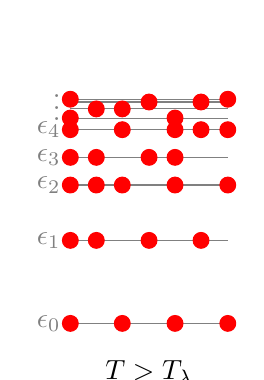
\begin{tikzpicture}
    \draw[gray] (2cm,0em) -- (0cm,0em) node[left] {$\epsilon_0$};
    \draw[gray] (2cm,3em) -- (0cm,3em) node[left] {$\epsilon_1$};
    \draw[gray] (2cm,5em) -- (0cm,5em) node[left] {$\epsilon_2$};
    \draw[gray] (2cm,6em) -- (0cm,6em) node[left] {$\epsilon_3$};
	\draw[gray] (2cm,7em) -- (0cm,7em) node[left] {$\epsilon_4$};
	\draw[gray] (2cm,7.42em) -- (0cm,7.42em) node[left] {$ $};
	\draw[gray] (2cm,7.75em) -- (0cm,7.75em) node[left] {$ $};
	\draw[gray] (2cm,8em) -- (0cm,8em) node[left] {$ $};
	\draw[gray] (2cm,8.1em) -- (0cm,8.1em) node[left] {$\vdots$};
	\draw[red,fill=red] (0.66cm,0em) circle (0.1cm);
	\draw[red,fill=red] (1.33cm,0em) circle (0.1cm);
	\draw[red,fill=red] (0cm,0em) circle (0.1cm);
	\draw[red,fill=red] (2cm,0em) circle (0.1cm);
	\draw[red,fill=red] (0cm,3em) circle (0.1cm);
	\draw[red,fill=red] (0.33cm,3em) circle (0.1cm);
	\draw[red,fill=red] (1cm,3em) circle (0.1cm);
	\draw[red,fill=red] (1.66cm,3em) circle (0.1cm);
	\draw[red,fill=red] (0cm,5em) circle (0.1cm);
	\draw[red,fill=red] (0.33cm,5em) circle (0.1cm);
	\draw[red,fill=red] (0.66cm,5em) circle (0.1cm);
	\draw[red,fill=red] (1.33cm,5em) circle (0.1cm);
	\draw[red,fill=red] (2cm,5em) circle (0.1cm);
	\draw[red,fill=red] (0cm,6em) circle (0.1cm);
	\draw[red,fill=red] (0.33cm,6em) circle (0.1cm);
	\draw[red,fill=red] (1cm,6em) circle (0.1cm);
	\draw[red,fill=red] (1.33cm,6em) circle (0.1cm);
	\draw[red,fill=red] (0cm,7em) circle (0.1cm);
	\draw[red,fill=red] (0.66cm,7em) circle (0.1cm);
	\draw[red,fill=red] (1.33cm,7em) circle (0.1cm);
	\draw[red,fill=red] (1.66cm,7em) circle (0.1cm);
	\draw[red,fill=red] (2cm,7em) circle (0.1cm);
	\draw[red,fill=red] (0cm,7.42em) circle (0.1cm);
	\draw[red,fill=red] (0.33cm,7.75em) circle (0.1cm);
	\draw[red,fill=red] (0.66cm,7.75em) circle (0.1cm);
	\draw[red,fill=red] (1cm,8em) circle (0.1cm);
	\draw[red,fill=red] (1.33cm,7.42em) circle (0.1cm);
	\draw[red,fill=red] (1.66cm,8em) circle (0.1cm);
	\draw[red,fill=red] (2cm,8.1em) circle (0.1cm);
	\draw[red,fill=red] (0cm,8.1em) circle (0.1cm);
	\draw (1cm,-1em) node[below] {$T>T_\lambda$};
    \end{tikzpicture}
    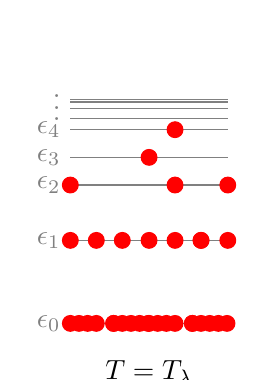
\begin{tikzpicture}
    \draw[gray] (2cm,0em) -- (0cm,0em) node[left] {$\epsilon_0$};
    \draw[gray] (2cm,3em) -- (0cm,3em) node[left] {$\epsilon_1$};
    \draw[gray] (2cm,5em) -- (0cm,5em) node[left] {$\epsilon_2$};
    \draw[gray] (2cm,6em) -- (0cm,6em) node[left] {$\epsilon_3$};
	\draw[gray] (2cm,7em) -- (0cm,7em) node[left] {$\epsilon_4$};
	\draw[gray] (2cm,7.42em) -- (0cm,7.42em) node[left] {$ $};
	\draw[gray] (2cm,7.75em) -- (0cm,7.75em) node[left] {$ $};
	\draw[gray] (2cm,8em) -- (0cm,8em) node[left] {$ $};
	\draw[gray] (2cm,8.1em) -- (0cm,8.1em) node[left] {$\vdots$};
	\draw[red,fill=red] (0cm,0em) circle (0.1cm);
	\draw[red,fill=red] (0.33cm,0em) circle (0.1cm);
	\draw[red,fill=red] (0.11cm,0em) circle (0.1cm);
	\draw[red,fill=red] (0.22cm,0em) circle (0.1cm);
	\draw[red,fill=red] (0.55cm,0em) circle (0.1cm);
	\draw[red,fill=red] (0.55cm,0em) circle (0.1cm);
	\draw[red,fill=red] (0.66cm,0em) circle (0.1cm);
	\draw[red,fill=red] (0.77cm,0em) circle (0.1cm);
	\draw[red,fill=red] (0.88cm,0em) circle (0.1cm);
	\draw[red,fill=red] (0.99cm,0em) circle (0.1cm);
	\draw[red,fill=red] (1cm,0em) circle (0.1cm);
	\draw[red,fill=red] (1.33cm,0em) circle (0.1cm);
	\draw[red,fill=red] (1.11cm,0em) circle (0.1cm);
	\draw[red,fill=red] (1.22cm,0em) circle (0.1cm);
	\draw[red,fill=red] (1.55cm,0em) circle (0.1cm);
	\draw[red,fill=red] (1.55cm,0em) circle (0.1cm);
	\draw[red,fill=red] (1.66cm,0em) circle (0.1cm);
	\draw[red,fill=red] (1.77cm,0em) circle (0.1cm);
	\draw[red,fill=red] (1.88cm,0em) circle (0.1cm);
	\draw[red,fill=red] (1.99cm,0em) circle (0.1cm);
	\draw[red,fill=red] (0cm,3em) circle (0.1cm);
	\draw[red,fill=red] (0.33cm,3em) circle (0.1cm);
	\draw[red,fill=red] (0.66cm,3em) circle (0.1cm);
	\draw[red,fill=red] (1cm,3em) circle (0.1cm);
	\draw[red,fill=red] (1.33cm,3em) circle (0.1cm);
	\draw[red,fill=red] (1.66cm,3em) circle (0.1cm);
	\draw[red,fill=red] (1.66cm,3em) circle (0.1cm);
	\draw[red,fill=red] (2cm,3em) circle (0.1cm);
	\draw[red,fill=red] (0cm,5em) circle (0.1cm);
	\draw[red,fill=red] (1.33cm,5em) circle (0.1cm);
	\draw[red,fill=red] (2cm,5em) circle (0.1cm);
	\draw[red,fill=red] (1cm,6em) circle (0.1cm);
	\draw[red,fill=red] (1.33cm,7em) circle (0.1cm);
	\draw (1cm,-1em) node[below] {$T=T_\lambda$};
  \end{tikzpicture}
  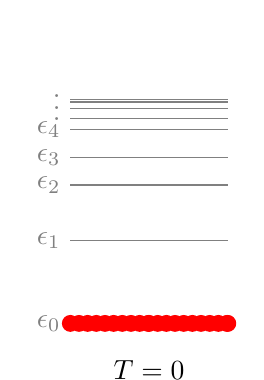
\begin{tikzpicture}
    \draw[gray] (2cm,0em) -- (0cm,0em) node[left] {$\epsilon_0$};
    \draw[gray] (2cm,3em) -- (0cm,3em) node[left] {$\epsilon_1$};
    \draw[gray] (2cm,5em) -- (0cm,5em) node[left] {$\epsilon_2$};
    \draw[gray] (2cm,6em) -- (0cm,6em) node[left] {$\epsilon_3$};
	\draw[gray] (2cm,7em) -- (0cm,7em) node[left] {$\epsilon_4$};
	\draw[gray] (2cm,7.42em) -- (0cm,7.42em) node[left] {$ $};
	\draw[gray] (2cm,7.75em) -- (0cm,7.75em) node[left] {$ $};
	\draw[gray] (2cm,8em) -- (0cm,8em) node[left] {$ $};
	\draw[gray] (2cm,8.1em) -- (0cm,8.1em) node[left] {$\vdots$};
	\draw[red,fill=red] (0cm,0em) circle (0.1cm);
	\draw[red,fill=red] (0.33cm,0em) circle (0.1cm);
	\draw[red,fill=red] (0.11cm,0em) circle (0.1cm);
	\draw[red,fill=red] (0.22cm,0em) circle (0.1cm);
	\draw[red,fill=red] (0.44cm,0em) circle (0.1cm);
	\draw[red,fill=red] (0.55cm,0em) circle (0.1cm);
	\draw[red,fill=red] (0.66cm,0em) circle (0.1cm);
	\draw[red,fill=red] (0.77cm,0em) circle (0.1cm);
	\draw[red,fill=red] (0.88cm,0em) circle (0.1cm);
	\draw[red,fill=red] (0.99cm,0em) circle (0.1cm);
	\draw[red,fill=red] (1cm,0em) circle (0.1cm);
	\draw[red,fill=red] (1.33cm,0em) circle (0.1cm);
	\draw[red,fill=red] (1.11cm,0em) circle (0.1cm);
	\draw[red,fill=red] (1.22cm,0em) circle (0.1cm);
	\draw[red,fill=red] (1.55cm,0em) circle (0.1cm);
	\draw[red,fill=red] (1.44cm,0em) circle (0.1cm);
	\draw[red,fill=red] (1.66cm,0em) circle (0.1cm);
	\draw[red,fill=red] (1.77cm,0em) circle (0.1cm);
	\draw[red,fill=red] (1.88cm,0em) circle (0.1cm);
	\draw[red,fill=red] (1.99cm,0em) circle (0.1cm);
	\draw[red,fill=red] (2cm,0em) circle (0.1cm);
	\draw (1cm,-1em) node[below] {$\phantom{T_\lambda}T=0\phantom{T_\lambda}$};
  \end{tikzpicture}
  \caption{\label{fig:beclevels}Schematic depiction of Bose-Einstein condensation. The ground state $\epsilon_0$ becomes macroscopically occupied as the temperature is reduced to below the critical temperature for condensation. In the limit of $T=0$ all bosons occupy the ground state.}
\end{figure}

Consider a gas of non-interacting bosons in thermal equilibrium at temperature $T$. The thermal de Broglie wavelength for each particle characterises the spatial extent of its localised wavepacket, and is conventionally defined by
\begin{equation}
\lambda_{\rm dB} = \sqrt{\frac{2\pi \hbar^2}{mk_{\rm B}T}},
\label{eq:debroglie}
\end{equation}
where $m$ is the mass of the particle and $\hbar$ is the reduced Plank constant. The de Broglie wavelength is inversely proportional to the square root of the temperature $T$, so that at high temperatures the wavepacket of each particle is small compared to the average inter-particle distance. Here classical, particle-like behaviour dominates the dynamics of the gas and the particles approximately follow the classical Boltzmann distribution. As the temperature of the gas is reduced, the wavelength associated with the particles grows. At a critical temperature, $T_\lambda$, the wavelength for each particle becomes comparable to the average inter-particle distance and the individual characteristics of particles are no longer apparent. Here the particles become indistinguishable and the idea of a particle trajectory no longer makes sense. The particles behave in a truly quantum manner and form a degenerate gas. The critical temperature for which this process occurs marks the onset of Bose-Einstein condensation.

For a gas of identical non-interacting Bosons in a uniform three-dimensional system of volume $V$ and number density $n=N/V$, Bose-Einstein condensation occurs when $n\lambda_{\rm dB}^3 \leq \zeta(3/2)$ \cite{Pethick,huang1987statistical}, where $\zeta(3/2)\approx2.612$ is the Riemann zeta function evaluated at $3/2$. By using this relation with Equation \ref{eq:debroglie} one finds the critical temperature,
\begin{equation}
T_\lambda = \frac{2\pi\hbar^2}{mk_{\rm B}} \left ( \frac{n}{\zeta(3/2)} \right )^{2/3},
\label{eq:tlambda}
\end{equation}
for the onset of Bose-Einstein condensation. The fraction of bosons condensed into the ground state, termed the condensate fraction, then be calculated as a function of temperature,
\begin{equation}
	\frac{N_0}{N} = 1 - \left( \frac{T}{T_\lambda}\right )^{3/2}.
\end{equation}

\section{Superfluid helium}
Many concepts relating to Bose-Einstein condensation and quantum gases were developed in the context of liquid $^4$He. Liquid helium is interesting in that when cooled to very low temperatures, the liquid does not crystallise or solidify at atmospheric pressures. In fact a pressure of over $25$ atmospheres is required to solidify $^4$He, even at its lowest temperatures \cite{Pethick}. 

Around 1930, Keesom {\it et. al} \cite{Keesom27,Keesom35} observed that when cooling liquid $^4$He, there exists a critical temperature known as the lambda point ($T_\lambda = 2.17$ K) at which the fluid undergoes a phase transition into a state known as helium II. It was later discovered by Kapitza \cite{Kapitza}, Allen and Misener \cite{Allen38} that helium II exhibits inviscid flow (one of several remarkable properties of helium II), and the fluid was deemed a ''superfluid''.

London \cite{London38,London38b} was the first to interpret the properties of helium II as a manifestation of Bose-Einstein condensation of helium atoms, but the idea was not widely accepted at first. The strongly-interacting liquid of helium atoms is a world away from Einstein's non-interacting gas of bosons. Instead, the two-fluid model of Landau \cite{Landau41} was the first successful description of helium II hydrodynamics, wherein two fluids exist alongside one another with densities depending on the temperature: an inviscid superfluid component and a viscous normal fluid component. At $T=T_\lambda$, the normal fluid makes up the entire fluid and there is no superfluid component. As the temperature is decreased, the proportion of the normal fluid decreases and that of the superfluid increases, such that at $T=0$ the fluid is entirely superfluid.

\subsection{Dispersion relation and excitations}
Landau showed that superfluid behaviour can be accounted for by a dispersion relation that is linear at low momenta \cite{Landau41}. Bogoliubov then showed that a weakly-interacting Bose gas supports exactly such a dispersion law \cite{bogo47}. This link between bosonic gases and helium II was a strong indicator that Bose-Einstein condensation was indeed the fundamental mechanism behind superfluidity, and finally gave traction to London's theory. Onsager \cite{Onsager49} and Feynman \cite{Feynman55} then predicted quantised circulation as an extension to London's work.

While Bose-Einstein condensation is now known to be the driving force behind helium II superfluidity, the strong interactions inherent in liquid helium restricts the condensed fraction of helium atoms to less than $10\%$ \cite{Donnelly} (even in the limit of zero temperature) and so a weakly-interacting Bose gas provides only a qualitative model of helium II superfluidity.

\begin{figure}
	\centering
	\begin{tikzpicture}
		\begin{axis}[samples=300,ylabel near ticks,xlabel near ticks,
				width=0.4\linewidth,
				height=0.45\linewidth,
				xlabel=$p$,
				ylabel=$\epsilon$,
				xmin=0,
				xmax=13,
				ymin=0.4,
				ymax=12,
				axis line style={-Latex[round]},
				axis y line*=left,
        axis x line*=bottom,
        yticklabels={,,},
        xticklabels={,,},
				major tick length = 0.00cm]
				\addplot[mark=none,thick,domain=0:12] {x^(0.25)*((x/2-4)*sin(deg(x/2-4)) + 4)};
		\end{axis}
	\end{tikzpicture}%
	\caption{\label{fig:hedisp}The dispersion relation for superfluid $^4$He, demonstrating the spectrum of elementary excitations. The linear dispersion of phonons can be seen at low momenta and the roton minimum at higher momenta.}
\end{figure}

The dispersion relation for liquid helium $^4$He is shown in Figure \ref{fig:hedisp}. For small momenta the relation is indeed linear. The fundamental excitations associated with this part of the relation are sound waves, known as {\it phonons}. For larger momentum, however, $\epsilon(p)$ exhibits an approximately quadratic shaped dip and local minimum. The fundamental excitations of this part of the relation are known as {\it rotons}, with the centre of the dip corresponding to the smallest possible energy of a roton, the {\it roton minimum}. 

\section{Dilute weakly-interacting atomic gases}
Gases of alkali atoms such as rubidium, sodium and lithium are ideal candidates for condensation: they are weakly-interacting, can be easily trapped magnetically, and readily cooled using lasers. When considering these gases, Einstein's ideal gas predictions provide a good estimate of the critical temperature for Bose-Einstein condensation.  However, as the gas is cooled towards the critical temperature it is necessary to avoid the transition into a liquid or solid. This can be done by reducing the atomic density such that the gas is dilute enough that elastic binary collisions in the gas dominate over three-body collisions. The required atomic densities are around $n \sim 10^{14}~{\rm cm}^{-3}$ \footnote{Compare this to the density of dry air at room temperature and pressure, $n \sim 10^{19}~{\rm cm}^{-3}$.}, and so by using Equation \ref{eq:tlambda} one predicts that the ultra-low temperatures of $T \sim 10^{-6}~{\rm K}$ are required for the onset of Bose-Einstein condensation.

\subsection{Experimental realisation}
The requirement of such low temperatures delayed the realisation of a true atomic BEC until 1995, when advances in atom cooling and trapping \cite{billphillips,chu98,Cohen-Tannoudji} lead to the condensation in vapours of rubidium ($^{87}$Rb) by the group of Professors Carl Wieman and Eric Cornell at the University of Colorado \cite{Anderson198}, and sodium ($^{23}$Na) by the group of W. Ketterle at MIT \cite{PhysRevLett.75.3969}. Wieman, Cornell and Ketterle were awarded the 2001 Nobel Prize in Physics for ``{\it the achievement of Bose-Einstein condensation in dilute gases of alkali atoms, and for early fundamental studies of the properties of the condensates}'' \cite{nobel01}.

A variety of cooling techniques, including laser \cite{billphillips,chu98,Cohen-Tannoudji} and evaporative \cite{PhysRevB.34.3476} cooling, originally developed in the attempt to condense spin-polarised hydrogen \cite{Hecht59, PhysRevLett.44.164, Silvera86}, are used to reach the ultra-low temperatures required for atomic Bose-Einstein condensation \cite{Pethick,RevModPhys.74.1131,RevModPhys.74.875}. A typical atomic condensate begins life as around $10^9$ atoms which are cooled to around 1K by a Zeeman slower: a laser beam propagating opposite to the atom flow reduces the velocity of the atoms from around $800~\rm{m/s}$ to $30~\rm{m/s}$. The atoms are transferred to a magneto-optical trap (MOT) formed by laser beams and magnetic fields and further cooled through Doppler cooling, where the Doppler effect is employed to reduce the momentum of atoms. A limit of this method is reached at around $1\,\mu$K \cite{Pethick} at which point evaporative cooling is required to cool the gas even further. Here the confining trap is carefully modified so that the high energy atoms escape the system. The remaining lower energy atoms rethermalise at a reduced temperature and lower density due to the loss of atoms. Using this technique, the gas can be cooled to the nK regime. The BEC then emerges marked by a very narrow velocity distribution for the atoms, indicating a macroscopic occupation of the ground state. 

Since the first experiments in 1995, an explosion of ultra-cold atomic physics has followed. Many species of atom are now routinely condensed by over 100 experimental groups all over the world. The list grows continuously: many alkalis \cite{Anderson198,PhysRevLett.75.3969,PhysRevLett.75.1687,PhysRevLett.78.985,PhysRevLett.85.1795,Modugno,Robert461,Weber232}, calcium \cite{PhysRevLett.103.130401}, dysprosium \cite{PhysRevLett.107.190401}, strontium \cite{PhysRevLett.103.200401,PhysRevLett.103.200402, PhysRevA.82.041602, PhysRevA.81.051601}, ytterbium \cite{PhysRevLett.91.040404}, chromium \cite{PhysRevLett.94.160401}, spin-polarised hydrogen \cite{PhysRevLett.81.3811}, metastable helium \cite{PhysRevLett.86.3459}, magnons \cite{Mathew11}, exciton-polaritons \cite{Kasprzak06} and even mixtures of different species \cite{PhysRevLett.89.053202, PhysRevLett.89.190404, PhysRevLett.100.210402,PhysRevA.84.011603}. Each species expands the richness of the fascinating phenomena available to experimentalists, with their unique atomic properties and range of interactions.

The experimental advances of controlling the trapping potential has allowed for direct interaction with the condensate using time-dependent magnetic fields and lasers. Localised laser beams can punch a `hole' in a condensate to create almost arbitrarily shaped obstacles \cite{Henderson09}. Exotic trapping potentials such as ring traps \cite{persistent,Ramanathan11}, uniform box traps \cite{gaunt_2013,chomaz_2015}, optical lattices \cite{Greiner02} and double-well \cite{PhysRevLett.106.025302} potentials can be realised with relative ease. The route has even opened to experimentation in reduced dimensionality \cite{Gorlitz,PhysRevLett.87.080403,PhysRevLett.91.250402,PhysRevLett.92.173003}. By significantly trapping the gas along one dimension it is possible to make a disc shaped, effectively two dimensional condensate, useful \cite{Neely,Freilich2010} for the study of vortex dynamics. A further trapping along a second dimension creates an elongated, effectively one dimensional condensate such that solitons, one-dimensional non-dispersive waves, become supported \cite{drazin1989solitons,PhysRevLett.101.120406}.

\subsection{Scattering length and interactions}
The atomic binary collisions in ultra-cold dilute gases are characterised by the $s$-wave scattering length, $a_s$. Higher energy $p$-wave and $d$-wave scattering is suppressed. Geometrically, a positive $a_s$ (as in a rubidium or sodium BEC) can be thought of as a measure of the effective radius of repulsive atoms. For gases with density in the region required, $n^{1/3}a_s \ll 1$, and so $a_s$ is much smaller than the average inter-atomic distance. This implies that the gas is weakly-interacting and around $99\%$ of the atoms can become Bose-condensed, resulting in a condensate fraction much greater than the theoretical maximum for helium II. This makes ultra-cold dilute atomic gases the purest form of BEC that can also be easily controlled and manipulated in the lab.

The scattering length may also be negative (as in a lithium BEC \cite{PhysRevLett.75.1687, PhysRevLett.78.985}). In this case the atoms are attractive, rather than repulsive, and the BEC is only stable up to a certain atom number. Importantly, it is possible to control the inter-atomic interaction, and therefore the scattering length, through the entire range of the parameter space using techniques such as {\it Feshbach resonance} (theoretically laid out in \cite{weiner2003cold} and experimentally demonstrated in \cite{Inouye1998,PhysRevLett.82.2422,PhysRevLett.85.1795}), providing further experimental control over the BEC.

With the unique level of purity and control available in the lab, weakly-interacting dilute atomic gases have become the ideal test-bed for studying Bose-Einstein condensation and for observation of quantum effects on a macroscopic scale.


\section{Macroscopic nonlinear excitations: vortices and solitons}
The rise of interest in Bose-Einstein condensation has led to a great amount of theoretical work. It can be argued that the greatest success in this area is the development of an effective mean-field theory which provides the so-called Gross-Pitaevskii equation (GPE) \cite{Pethick,Pitaevskii61,Gross61,RevModPhys.71.463}, a classical evolution equation and a variant of the nonlinear-Schr\"odinger equation used in many areas of physics, including plasma physics \cite{PhysRevLett.37.693} and non-linear optics \cite{PhysRevA.65.053614,borisSolitons}. The GPE is much simpler than modelling a BEC using the full many-body Schr\"oedinger equation, yet accurately captures the statics and dynamics \cite{RevModPhys.71.463,Denschlag97, Burger99, PhysRevLett.86.2926, Dutton27072001,vortices,lobo_2004,PhysRevLett.85.2857} of a BEC over a range of realistic experimental parameters. Section \ref{cha:theoretical_model} describes the mean-field formulation  in detail and formally derives the GPE from the starting point of the many-body Schr\"oedinger equation.

The non-linearity in the GPE arises from atom-atom interactions and gives rise to a great deal of interesting effects, both from a mathematical standpoint and when modelling an atomic BEC. A selection of the interesting and experimentally relevant non-linear phenomena are described in this section.

\subsection{Vortices}
A family of non-linear excitations supported by the GPE are {\it quantum vortices}, which arise via topological defects in the wavefunction that parametrises the condensate. Solutions with quantum vortices contain structures identified by a localised density dip, the vortex core, masking a phase singularity in its centre. The phase singularity forms a velocity field such that fluid circulates around the vortex core.

Quantum vortices are carriers of vorticity in an irrotational superfluid system, and can arise both naturally during the formation of a BEC or by direct interaction with a condensate. A standard method of generating vortices, relevant to atomic condensates and helium II, is by rotation of the superfluid \cite{PhysRevLett.43.214,PhysRevLett.84.806,hodby_2002,Abo-Shaeer476, PhysRevLett.87.210403}. At lower angular speeds the rotation has no effect, however, above a critical value the presence of vortices lowers the energy of the system \cite{0953-8984-13-12-201,NozieresPines}. In this case, one or more vortices nucleate into the system, forming a lattice \cite{PhysRevLett.43.214,Abo-Shaeer476} at the centre of rotation. Another example is the formation of vortices as a result of broken symmetry after a fast quench into the BEC regime. Through the Kibble-Zurek mechanism \cite{0305-4470-9-8-029,Zurek85,KZvort99}, pockets of phase coherence form, separated in space. As the phase coherence grows in the condensate, boundaries are created and discontinuities along these boundaries leads to the formation of vortex lines. Further methods of generating vortices include artificial phase imprinting \cite{Cornell99,Dobrek99,Leanhardt99} of the topological defect via laser light, or by stirring a BEC with a localised laser beam \cite{PhysRevLett.84.806,hodby_2002,Abo-Shaeer476,jma00,Raman01,Inouye}.

Quantised vortices have much in common with the classical vortices observed in nature. However, while classical vortices can be created with any degree of fluid rotation, characterised by the circulation $\Gamma$, quantised vortices differ in that their circulation is constrained (as a direct consequence of quantum mechanics) to integer multiples of the {\it quantum of circulation}, $\kappa$, with a value dependent on the system.

Experimentally, quantum vortices have been observed in many different configurations and for various trap geometries. Quantised vortex lines \cite{Dutton27072001}, vortex rings \cite{PhysRevLett.86.2926}, vortex tangles \cite{Henn}, quasi-two-dimensional turbulence \cite{kwon_moon_14}, vortex lattices \cite{PhysRevLett.84.806,Abo-Shaeer476,abo_shaeer_2002,PhysRevLett.86.4443}, vortex dipoles \cite{Neely}, giant vortices \cite{PhysRevLett.90.170405}, and multiply charged vortices \cite{PhysRevLett.93.160406} have all been realised in BECs. The condensate is observed via imaging of the atomic gas density, but the vortex core size is typically smaller than the imaging resolution. To overcome this the condensate is expanded by releasing it from the trap prior to imaging. The vortices then appear as localized regions of low density in the expanded condensate images.

Quantum vortices have also been observed in superfluid helium \cite{Vinen218}. In 1979, the first clear and direct image of a quantised vortex lattice in rotating helium II was provided by Packard {\it et. al} \cite{PhysRevLett.43.214}. Electrons were trapped inside vortex cores and accelerated towards a florescent screen to mark the position of the vortex. The resulting images are shown in Figure \ref{fig:hevorts} for different rotation speeds. More recently, there has been a significant advance by Lathrop {\it et al} \cite{Bewley09}. Here vortex lines were visualised and tracked in helium II by using tracer particles of frozen hydrogen.

\begin{figure}
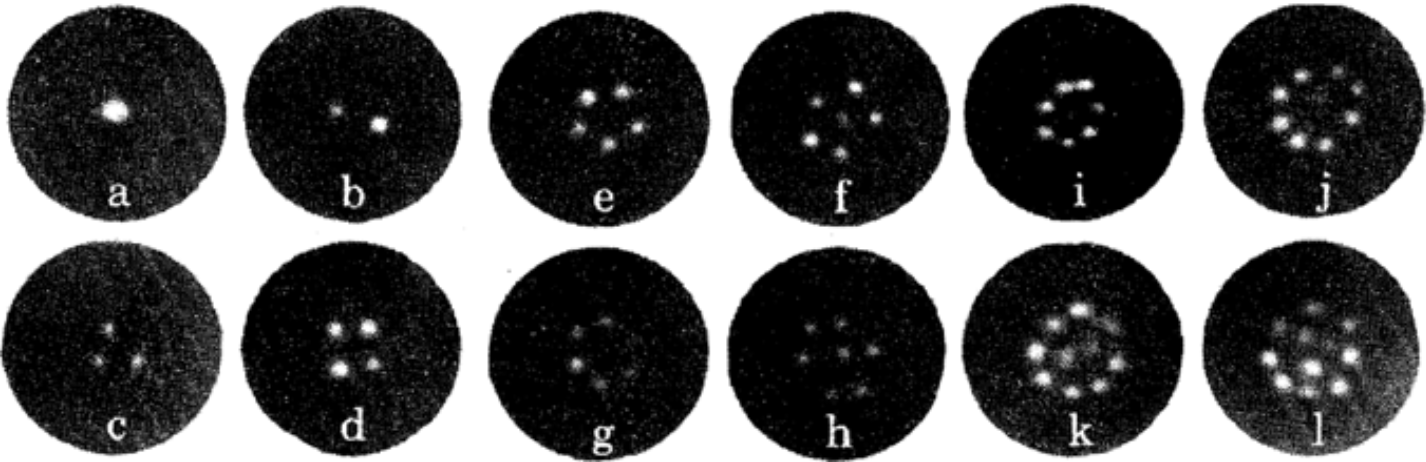
\includegraphics[width=\linewidth]{intro/packard}
\caption{\label{fig:hevorts} Results of the superfluid helium experiments of Packard \cite{PhysRevLett.43.214}, with (a-l) corresponding to increasing rotation velocities of the helium II container. Vortex line position is marked by the glowing dots.}
\end{figure}

\subsection{Solitons}
Solitons are a non-linear localised excitation, supported by the one dimensional GPE. Soliton solutions contain localised propagating wavepackets that are self-reinforcing due to the non-linearity of the system balancing dispersive effects. When in a homogeneous medium they travel at zero or finite constant speed, and have the property that they undergo non-destructive collisions. There are two species of soliton, bright \cite{PhysRevA.62.063611} and dark solitons \cite{PhysRevA.62.063610}. Their behaviour in optics, leading to a bright collection or dark absence of light, is the origin of these names. Solitons are an active area of research in several diverse areas of non-linear mathematics and physics \cite{drazin1989solitons,remoissenet2013waves}, and are well known for their applications in optical and fluid systems \cite{yu_kivshar_1998}. For these reasons solitons have been of great interest \cite{kevrekidis2007emergent,1751-8121-43-21-213001} since the first experimental realisation of atomic BECs.

In three-dimensional BECs, solitons take the form of solitonic waves, but are not solitons in the strict mathematical sense; the structures are unstable and proceed to decay \cite{Burger99,PhysRevA.62.053606,PhysRevA.65.043612,Tikhonenko96}. In weakly-interacting BECs with quasi-1D geometries, however, solitons are stable and have been observed with long lifetimes and with behaviour in agreement with numerical simulations \cite{PhysRevLett.101.120406}.

\subsubsection{Bright solitons}
Bright solitons arise in fluid \cite{Russell45}, plasma \cite{PhysRevLett.37.693,PhysRevLett.33.886}, acoustical \cite{naugolnykh1998nonlinear}, and optical physics \cite{agrawal2001nonlinear} and can be easily pictured by the classical example of a hump travelling along the surface of shallow water, as first reported in 1845 \cite{Russell45}. The non-dispersal and destruction-less collision properties of bright solitons make them particularly important in applications for optical communications \cite{hasegawa1995solitons}.

Bright solitons are supported in condensates for the case of effectively attractive interactions ($a_s < 0$) \cite{PhysRevA.62.063611}, were first generated and experimentally observed with lithium \cite{Strecker02,Khaykovich1290} in quasi-one-dimensional traps.

\subsubsection{Dark solitons}
In general, dark solitons are less prevalent than the bright species, but are of particular interest in the context of weakly-interacting BECs as they are are formed in the case of repulsive interactions ($a_s > 0$) \cite{PhysRevA.62.063610}. They consist of a density dip and phase slip \cite{dodd1982solitons} of varying size, depending on the speed of the soliton propagation. Dark solitons were first realised in 1987 in non-linear optics \cite{Emplit87}, followed by their creation in shallow liquids \cite{PhysRevLett.64.1518}, as discrete mechanical standing waves \cite{PhysRevLett.68.1730}, and in magnetic films \cite{PhysRevLett.70.1707}.

More recently, dark solitons have been engineered in repulsive atomic BECs in a controlled manner through phase imprinting methods \cite{Denschlag97,Burger99,PhysRevLett.86.2926,PhysRevLett.101.120406} and by perturbing the condensate density. They have also been produced through dynamical processes \cite{Weller08,PhysRevLett.99.160405}, such as by sweeping a laser beam through the condensate \cite{PhysRevLett.99.160405}. 

Dark solitons that have been generated in higher than quasi-1D geometries have been observed to decay into vortex rings \cite{PhysRevLett.86.2926,Dutton27072001,Shomroni09}, due to their known instability to transverse excitations.


\section{Quantum turbulence}
Classical turbulence is a complicated flow regime characterised by chaotic and highly irregular flow and the appearance of unsteady vortices on many length scales interacting with one another. In classical isotropic turbulence, most of the kinetic energy is contained in large-scale structures and is distributed following the famous Kolmogorov energy spectrum \cite{davidson2004turbulence}.

{\it Quantum} turbulence is a state dominated by an irregular tangle of quantised vortex lines. The quantised circulation and inviscid flow characteristics of superfluidity provides a simplified platform to study complicated vortex dynamics in general, and so the nature of turbulence in superfluids is the subject of much experimental and theoretical study \cite{Bradley11,skebek12,PhysRevLett.110.014502,barenghi_skrbek_14,PhysRevLett.115.155303}. Despite the fundamental differences between superfluids and classical fluids, the observations of Kolmogorov energy spectra in superfluid turbulence are suggestive of a deep connection between them \cite{barenghi_skrbek_14}. 

\subsection{Turbulence in helium II}
Quantum vortices are carriers of vorticity in superfluids and play an important role in the behaviour of the superfluid component of helium II. They have been experimentally and theoretically studied in helium II from around 1950 \cite{Donnelly}, but clearly visualising the three dimensional nature of individual vortex lines and reconnections remained a challenge until fairly recently \cite{Bewley09,Fonda12}: the large normal fluid component and a vortex core size of only a few Angstr\"oms limits visualisation techniques.

A large disordered collection of vortex lines is thought to be the driving force of the turbulence. However, within the tangle the vortex core size is small compared to the average inter-vortex spacing. For this reason the standard method of modelling of vortex dynamics at large-scales is handled by approximating the vortices as infinitesimally thin vortex filaments, with motion described by the Biot-Savart law \cite{barenghi_donnelly_01}. The limitation of the vortex filament model is that all phenomena that occur on the length-scale of the vortex core (of which we are interested in) is lost. Features like vortex reconnection can be manually introduced into this model \cite{barenghi_donnelly_01}, but the full microscopic description is lost.

On the other hand, the GPE model for a weakly-interacting Bose gas provides a microscopic model of helium II on a qualitative level. As already discussed, the strongly-interacting helium atoms, existence of high momenta rotons, and relatively low fraction of condensed helium atoms limits the accuracy of the model. Nevertheless, the GPE excels at describing the micro-scale phenomena such as vortex nucleation \cite{frisch92}, reconnections \cite{PhysRevLett.71.1375, PhysRevLett.76.4745}, sound emission \cite{leadbeater,PhysRevA.69.053601}, and Kelvin wave excitation, and so we will use the GPE at various points throughout this thesis to model helium II dynamics.

Typically turbulence in helium II is generated using mechanical methods, creating turbulence with oscillating obstacles, including grids \cite{Davis2000}, wires \cite{Guenault1986,Bradley2011,Fisher2001}, spheres \cite{Schoepe1995} and others \cite{Blaauwgeers2007,Bradley2012,Tabeling1998,Salort,VinenSkrbek2008}. Methods without the use of oscillating structures have been also been devised, such as the use of heat flux \cite{Vinen114} or container spin-down \cite{PhysRevLett.99.265302}, to generate turbulence . A mutual friction \cite{Donnelly} couples the normal fluid and superfluid components, and at finite temperature leads to a dissipation of the resulting turbulent vortex tangle. In the limit of very low temperatures the mutual friction tends to zero. It is expected that in this limit Kelvin wave excitations \cite{leadbeater,PhysRevA.69.053601} and vortex reconnections leads to dissipation via sound waves, but the entire mechanism is not yet fully understood \cite{PhysRevB.61.1410}.

\subsection{Turbulence in BECs}

Weakly interacting atomic BECs present a key improvement over helium II superfluidity for the study of quantum turbulence. Although the spatial extent of BECs support much fewer vortices than for superfluid helium, the structure of individual vortices and their turbulent dynamics can be experimentally resolved much easier. This is due to the relatively large vortex core size, on the scale of a micron, available to atomic BECs and the fact that the state of the entire atomic gas can be readily visualised through imaging techniques. Expansion imaging has provided a technical leap in this area, allowing individual vortex cores and reconnection events to be directly observed \cite{PhysRevLett.84.806,Raman01,kwon_moon_14}. Improved real time and non-destructive imaging of condensates is now possible \cite{Freilich2010} by out-coupling of a small representative fraction of the gas for each image, allowing for observation of quantum vortex trajectories. A further recent improvement in this area \cite{powis} has allowed for the imaging of vortex polarity as well as its location in space. These technical leaps in imaging have made atomic condensates an extremely attractive medium for exploring quantum vortex turbulence. 

The range of length scales available to classical turbulence and superfluid helium turbulence far outshines those currently available to atomic BECs, and much theory of classical turbulence is defined by the distribution of kinetic energy over the large number of length scales available. Nevertheless, numerical studies show quantum turbulence can distribute the kinetic energy in an atomic condensate in agreement with Kolmogorov's $k^{-5/3}$ law \cite{Nore,Kobayashi,PhysRevLett.103.084501}.

\section{Thesis overview}
An outline of the thesis structure and a brief description of each chapter is given in this section. The thesis is split into three main parts. Part I introduces the formalism, models and numerical tools that we go on to use in part II to model quantum fluids and generate numerical results. Part III is a collection of appendices. The following publications feature partially some of the results shown in the thesis, and the collaborative contributions are highlighted here.
\begin{itemize}
	\item Quantum analogues of classical wakes in Bose-Einstein condensates\\
	{\footnotesize G. W. Stagg, N. G. Parker and C. F. Barenghi, J Phys B: At. Mol. Opt. Phys. {\bf 47} 095304 (2014)}
	\item Generation and decay of two-dimensional quantum turbulence in a trapped Bose-Einstein condensate\\
	{\footnotesize G. W. Stagg, A. J. Allen, N. G. Parker and C. F. Barenghi, Phys. Rev. A {\bf 91}, 013612 (2015)}
	\item Classical-like wakes past elliptical obstacles in atomic Bose-Einstein condensates\\
	{\footnotesize G. W. Stagg, A. J. Allen, C. F. Barenghi, N. G. Parker, J. Phys.: Conf. Ser. {\bf 594} 012044 (2015)}
	\item Critical velocity of a finite-temperature Bose gas\\
	{\footnotesize G. W. Stagg, R. W. Pattinson, C. F. Barenghi, N. G. Parker, Phys. Rev. A {\bf 93}, 023640 (2016)}
	\item A superfluid boundary layer\\
	{\footnotesize G. W. Stagg, N. G. Parker, C. F. Barenghi, arXiv:1603.01165 (2016)}
\end{itemize}

\subsubsection{Part I - Introduction and Theory}
Chapter 1 introduces the concept of Bose-Einstein condensation, superfluidity, and the nature of quantum turbulence in weakly interacting atomic condensates and superfluid liquid helium.

Chapter 2 describes the theoretical concepts and mean-field methodology that allows us to efficiently model a dilute, weakly interacting atomic Bose gas at zero and finite temperatures. We describe the Gross-Pitaevskii equation (GPE), a non-linear Schr\"odinger equation used to model condensates at zero temperature, and go on to extend the GPE to take into account finite temperature effects through phenomenological damping or the classical-field method. We detail some of the consequences of the model, such as quantised circulation, and show various initial conditions and simple solutions of the GPE.

Chapter 3 details the theory and implementation of various numerical procedures we use to generate the simulations and results shown in part II. The time-stepping numerical solver is described, followed by an extensive description of vortex locating and tracking. Finally a method is described for the filtering of the thermal part of the field when using the classical-field method.

\subsubsection{Part II - Numerical Studies}
Part II consists of a selection of the numerical simulations we have performed, interpretations of the results and any applications to real experimental systems. Chapter 4 extends recent studies of moving obstacles in superfluids, a system mimicking a well known problem for classical viscous flows. We present numerical simulations of classical-like wakes, consisting of vortex clusters, generated by the presence of elliptical obstacles.

Chapter 5 was motivated by the recent experimental work of Kwon {\it et al.} \cite{kwon_moon_14}. We model their experimental set up in which a trapped condensate is translated past an obstacle, and study the decay of the resulting 2D quantum turbulence and vortex annihilation events. Communications with Y. Shin and A. Cidrim were helpful in the interpretation of the numerical simulations shown in this chapter.

Chapter 6 was motivated by further work of Kwon {\it et al.} \cite{kwon_2015a}, highlighting the need to extend the study of the critical velocity for vortex nucleation to finite temperatures. We use classical field methods to simulate finite temperature homogeneous Bose gases. We simulate the gas from a strongly non-equilibrium initial distribution, and classify the nature of the resulting turbulent vortex tangle. The previous numerical work of A. J. Youd was helpful in the development of our classical-field code, used in this chapter.

Chapter 7 is inspired by recent experimental studies in helium II, generating turbulence with oscillating obstacles such as wires, spheres and grids \cite{Davis2000,Guenault1986,Bradley2011,Fisher2001,Schoepe1995,Blaauwgeers2007,Bradley2012,Tabeling1998,Salort,VinenSkrbek2008}. We simulate a quantum fluid in the presence of a real rough boundary obtained via atomic force microscopy \cite{Lawson}, with data kindly provided by C. R. Lawson. We find surprising evidence of the formation of a thin `superfluid boundary layer' consisting of vortex loops and rings.

In Chapter 8 we briefly review the main conclusions of the work shown in the thesis and discuss opportunities for further research in the area.

\subsubsection{Part III - Appendix}
Part III is a collection of appendices. Appendix A consists of various detailed derivations relevant to the theoretical modelling of an atomic BEC. Appendix B contains definitions of relevant quantities in our quantum fluid simulations. Appendix C is a collection of numerical algorithms that we have used.



\end{chapter}

  \begin{chapter}{\label{cha:theoretical_model}Theoretical Modelling of BEC}
\section{\label{section:meanfield} Mean-field description}
We aim to accurately model the dynamics of a closed system containing a dilute, weakly interacting Bose gas of $N$ atoms, at extremely low temperatures. One could model the entire system by constructing a N-body quantum wavefunction, which would follow the Schr\"odinger equation, but the complexity of this method makes it extremely unwieldy to model the large number of particles used in Bose-Einstein condensate (BEC) experiments happening all around the world.

We instead model the system with a mean-field theory, in which there are essentially two main approximations. Firstly, justified by the dilute property of the gas, any binary interaction between particles is assumed to be a contact delta function,
\begin{equation*}
V(\mathbf{r}-\mathbf{r}') = g \delta(\mathbf{r}-\mathbf{r}').
\end{equation*}
Interactions involving a higher number of particles are ignored. Secondly, we assume all particles in the condensate are macroscopically described by a single wavefunction, $\psi(\mathbf{r},t)$. As the particles all share the same phase and quantum state, $\psi(\mathbf{r},t)$ is a classical field. This second approximation also assumes that there are no particles contributing to thermal or quantum fluctuations beyond the classical field, and so is only strictly justified when the temperature, $T$, is exactly $0\mathrm{K}$.

\section{\label{section:gpe} The Gross-Pitaevskii Equation}
The result of this methodology is the Gross-Pitaevskii equation (GPE), 
\begin{equation}
\mathrm{i} \hbar \frac{\partial\Psi({\bf r},t)}{\partial t} = \left(-\frac{\hbar^2}{2m}\nabla^2 + V({\bf r},t) + g|\Psi({\bf r},t)|^2 - \mu \right) \Psi({\bf r},t),
\label{eq:gpe}
\end{equation}
where $V({\bf r},t) = V_{\mathrm{obj}}({\bf r},t) + V_{\mathrm{trap}}({\bf r},t)$. In the homogeneous case $V_{\mathrm{trap}}({\bf r},t)=0$, otherwise a harmonic trapping potential is used. In the case of a 3D spherically symmetric condensate the harmonic trapping potential is defined as $V_{\mathrm{trap}}({\bf r},t)=m\omega{\bf r}/2$.

The first two terms on the right hand side of the GPE are the energy of a single particle in a potential field $V$ and he third term describes the non-linear effects between the multiple particles in the system, with a strength usually parametrised by $g=4\pi N \hbar^2a/m$,
where $m$ is the mass of a single particle, $a$ is the s-wave scattering length and and $N$ is the number of particles.
Taking into account the fact that the GPE is only valid at $T=0$, it turns out the equation is surprisingly successful at quantitatively modelling ultra-cold gasses, even up to a temperature of $T=\frac{T_c}{2}$, where $T_c$ is the critical temperature for Bose-Einstein condensation. The GPE is also successful at qualitatively modelling BEC based effects in higher temperature superfluids, such as liquid helium II[CITE SOME WORK] and even in neutron starts [CITE SOME WORK].

A detailed explanation of the mean-field formulation of the model and the full derivation of the GPE is shown in Section \ref{appsection:gpeqft}.

\section{\label{section:gpedimless} Dimensionless Gross-Pitaevskii Equations}
	Bose-Einstein condensates can be formed with almost any size or scale. An ultra-cold BECs topology or atom interaction strength can be fairly easily changed with magnetic/optical potentials and Feshbach resonances. Superfluid helium can have vortex core sizes of $\sim$1 or $\sim$100 angstroms, depending on the isotope of helium used. The cores of neutron stars are even theorised to be superfluid. For this reason, it is desirable to rescale the length scales used in the GPE so that any of the calculations performed can be easily reformulated into any length scale desired. We make this process easier by doing all calculations with dimensionless parameters. Another advantage of the dimensionless formulation is that the size of the values involved are all normalised on the scale of unity, reducing the chance of errors in numerical computation due to the floating point representation used by modern computer architectures.
	We present two methods of making the GPE dimensionless, the specific scaling used is chosen by the needs of the simulation and is usually apparent (such as by whether a trapping potential is involved).

	\subsection{\label{section:gpedimlesshomg} Homogeneous GPE}
		Consider a homogeneous system with repulsive iterations and with $V_{\mathrm{trap}} = 0$. In this case, $\Psi$ does not depend on ${\bf r}$, nor on $t$, and so we can set the time and spacial derivatives in the GPE to zero,
		\begin{equation}
		0 = \left(g|\Psi({\bf r},t)|^2 - \mu \right) \Psi({\bf r},t).
		\end{equation}
		By rearranging, we can easily find the natural homogeneous density of the system: $\rho = |\Psi|^2 = \mu/g$. We then choose to rescale the wavefunction using this value, so that $\psi = \Psi/\sqrt{\rho}$.

		By dimensional arguments (see Appendix \ref{section:healing} for details), the length scale of space is the healing length, $\xi = \hbar/\sqrt{mg\rho}$, and the length scale of time $\tau = \hbar/(g\rho)$. These units are often called the `natural units'. We define the rescaled dimensionless quantities as
		\begin{equation}
			\tilde{t} = \frac{t}{\tau}, ~~~ \tilde{r} = \frac{r}{\xi}, ~~~ \tilde{\varepsilon} = \frac{\varepsilon}{\mu},
		\end{equation}
		for time, length, and energy respectively, where a tilde denotes a dimensionless quantity. Substituting the dimensionless quantities into Equation \ref{eq:gpe} leads to the homogeneous GPE,
		\begin{equation}\label{eq:dimgpehomg}
		\mathrm{i}\frac{\partial\psi({\tilde{\bf r}},\tilde{t})}{\partial {\tilde{t}}} = \left( -\frac{1}{2}\tilde{\nabla}^2 + |\psi({\tilde{\bf r}},\tilde{t})|^2 + \tilde{V}_{\mathrm{obj}}({\tilde{\bf r}},\tilde{t}) - 1 \right) \psi({\tilde{\bf r}},\tilde{t}).
		\end{equation}
		In the interests of neatness the dimensionless signifier tilde will be omitted in future discussions of the homogeneous GPE. Quantities used with the wavefunction symbol $\psi$ are to be regarded as inherently dimensionless through the natural units.

	\subsection{\label{section:gpedimlesstrap} Trapped GPE}
		When considering a harmonically trapped condensate it is convenient to work with a wavefunction with density normalised to unity, that is,
		\begin{equation}\label{eq:intwf}
			\int |\phi|^2 \mathrm{d}^3{\bf r} = 1,
		\end{equation}
		We non-dimensionalise Equation \ref{eq:gpe} in terms of the length scales using the harmonic oscillator length, $l = \sqrt{\hbar/(m\omega)}$. This leads to the dimensionless rescalings,
		\begin{equation}
			\hat{t} = t\omega, ~~~ \hat{r} = \frac{r}{l}, ~~~ \hat{\varepsilon}= \frac{\varepsilon}{\hbar\omega},
		\end{equation}
		for time, length, and energy respectively, where a hat denotes a dimensionless quantity.
		We find then that
		\begin{equation}
			\int |\Psi|^2 \mathrm{d}^3{\bf r} = N \Rightarrow \int |\Psi|^2 N^{-1} l^3\mathrm{d}^3\hat{\bf r} = 1,
		\end{equation}
		and so we rescale the wavefunction to satisfy Equation \ref{eq:intwf},
		\begin{equation}
			 |\phi|^2 = |\Psi|^2 N^{-1} l^3 \Rightarrow \phi = \Psi N^{-\frac{1}{2}} l^\frac{3}{2}.
		\end{equation}
	Substituting the new rescaled quantities into Equation \ref{eq:gpe} leads us to the trapped GPE,
	\begin{equation}\label{eq:dimgpetrapped}
		\mathrm{i}\frac{\partial\phi({\hat{\bf r}},\hat{t})}{\partial {\hat{t}}} = \left( -\frac{1}{2}\hat{\nabla}^2 + \hat{g}|\phi({\hat{\bf r}},\hat{t})|^2 + \hat{V}({\hat{\bf r}},\hat{t}) - \hat{\mu} \right) \phi({\hat{\bf r}},\hat{t}).
	\end{equation}
	where
	\begin{equation}
		 \hat{g} = \frac{gN}{\hbar \omega l^3}.
	\end{equation}
	In the interests of neatness the dimensionless signifier hat will be omitted in future discussions of the harmonically trapped GPE. Quantities used with the wavefunction symbol $\phi$ are to be regarded as inherently dimensionless through the harmonic oscillator units.

\section{\label{section:quasi2dgpe} Quasi-Two-Dimensional Gross-Pitaevskii Equation}
	For some condensate geometries it is useful to be able simulate the condensate via a lower dimensional GPE. An example of this is the highly oblate, sometimes called `pancake', condensate, in which the trapping potential is defined as
	\begin{equation}
		V_{\mathrm{trap}}(x,y,z)=m\omega_\perp^2\frac{x^2+y^2}{2} + m\omega_z^2\frac{z^2}{2},
	\end{equation}
	with trapping frequencies $\omega_z >> \omega_\perp$ and under the condition $\hbar\omega_z >> \mu$, where $\mu$ is the 3D chemical potential. Tight $z$ confinement causes the dynamics to become essentially two dimensional (experimentally achieved in \cite{Gorlitz}) as the wavefuntion along $z$ becomes fixed into the independent harmonic oscillator ground state, so that
	\begin{equation}
		\Psi({\bf r},t) = \Psi_\perp(x,y,t) \Psi_z(z).
	\end{equation}
	An expression for $\Psi_z$ is found by assuming a Gaussian ground state under the condition that $\int |\Psi_z(z)|^2 \mathrm{d}z=1$.
	\begin{equation}
		\Psi_z(z) = \pi^{-1/4} l_z^{-1/2} \exp\left(-z^2/2l_z^2\right),
	\end{equation}
  where $l_z=\sqrt{\hbar/m \omega_z}$. This is known as the quasi-2D regime and when this form of $\Psi$ is substituted into Equation \ref{eq:gpe} it forms a 2D-GPE that can be used to model the system with reduced dimensionality, with the modified interaction term $g_{\mathrm{2D}} = g/( \sqrt{2\pi}l_z)$ \cite{parkerthesis}. The 3D chemical potential $\mu$ is also modified as an extra term is absorbed, $\mu_\mathrm{2d} = \mu - \hbar\omega_z/2$, and all other three-dimensional properties become two-dimensional.

	A similar process can be performed with `sausage' or `cigar' quasi-1D geometries so that a 1D-GPE can be used with a modified $g_{\mathrm{1D}}$ interaction term, and $\mu_{\mathrm{1D}}$ chemical potential. As before all 3D properties become 1D, however as we will not consider experimentally accurate 1D cases in detail, the specifics are omitted from this thesis.


\section{\label{section:gpestationary} Time-independent Gross-Pitaevskii Equation}
 We find a stationary version of the GPE by first fixing the potential, $V({\bf r},t)$, so that it is constant in time, and then writing the wavefunction in the form $\Psi({\bf r},t) = \Psi_0({\bf r}) \exp (\mathrm{i}\mu t / \hbar)$, where $\Psi_0({\bf r})$ is the ground state. Equation \ref{eq:gpe} then becomes
	\begin{equation}\label{eq:stationgpe}
		\mu\Psi_0({\bf r}) = \left( -\frac{\hbar^2}{2m}\nabla^2 + V({\bf r}) + g|\Psi_0({\bf r})|^2  \right) \Psi_0({\bf r}),
	\end{equation}
	the time-independent GPE. In the absence of interactions, $g=0$, this reduces to the standard Schr\"odinger equation. This version of the GPE can be used to find stationary solutions of the system for a certain $\mu$ which characterises the energy of the ground state.
	
\section{\label{section:imagTime} The imaginary time propagation method}

	Many numerical explorations of quantum systems, particularly those associated with magnetic or optical trapping,  involve calculating the ground-state as either the final result or as a stepping stone for further calculations. While often there exists analytic solutions for a condensate ground state, this problem is often solved numerically using so called eigensolvers. Numerically finding the ground state becomes practically necessary if a simulation requires complicated potential fields.

	There are several methods available for implementing a numerical eigensolver: inverse iteration and Lanczos methods \cite{thijssen1999computational}, systematic variational techniques \cite{Bao2003230}, boundary eigenvalue methods \cite{Edwards95}, conjugate gradient techniques \cite{NumericalRecipes} and imaginary time propagation \cite{PhysRevE.62.7438}. We choose to use the last of these methods due to its relative simplicity at the expense of computational time.

	The imaginary time method revolves around moving from real to imaginary time using a Wick rotation $\tau = it$. The substitution transforms the GPE into a form similar to a diffusion equation. As a result, a local equilibrium can be found by propagating $\tau$. This can be understood by considering a trial solution (as similar to the true ground-state as possible) as a collection of eigenfunctions $\Psi_n$ corresponding to eigenvalues $E_n$,
\begin{equation*}
\Psi(\mathbf{r},\tau) = \sum_n \Psi_n(\mathbf{r})\exp\left(-\frac{E_n\tau}{\hbar}\right).
\end{equation*}
The eigenfunctions decay exponentially under propagation of the GPE in imaginary time. In particular, the decay rate is directly related to the size of the eigenvalues $E_n$, so that eigenfunctions relating to higher eigenvalues decay the fastest. The final ingredient is to inhibit the overall decay of the wavefunction by renormalising during propagation. After a sufficient transient time the contributions from the higher eigenvalues become negligible, forcing the wavefunction to tend towards the lowest energy eigenfunction,
\begin{equation*}
\Psi(\mathbf{r},\tau) \rightarrow \Psi_0(\mathbf{r})\exp\left(-\frac{E_0\tau}{\hbar}\right).
\end{equation*}
The imaginary time propagation method converges on the ground state solution very slowly and so we must perform many steps to prepare an initial state. A silver lining of this drawback is that the method can be used to prepare almost any viable initial state. For example, an initial condition consisting of a Thomas-Fermi profile with many vortices can be `smoothed' by fixing the phase during imaginary time propagation. The result is a less violent start to condensate dynamics as minimal sound is produced due to the difference between the approximate initial condition and a true solution of the GPE.

The energy can be used as a way to gauge the solution convergence. An example ground state solution is found using the imaginary time method and is shown with the energy in Figure \ref{fig_imagtimesolgs}. 
\begin{figure}
	\centering
   \begin{tikzpicture}
    \begin{axis}[
        width=0.6\linewidth,
        height=0.33\linewidth,
        xlabel=$-t\omega/i$,
        ylabel=$E/(\hbar\omega)$,
        restrict x to domain=0:1,
        colormap name=hsvcl,
        major tick length = 0.07cm
      ]
      \addplot gnuplot [raw gnuplot,mark=none,color=black,thick]{
      	plot "numerics/figures/imag-time-prop-energy.txt" using 2:3 with lines;
      };
    \end{axis}
  \end{tikzpicture}
  \hspace{0.04\linewidth}
  \begin{tikzpicture}
  \begin{axis}[
    width=0.33\linewidth,
    height=0.33\linewidth,
    axis on top,
    xmin=-9,
    xmax=9,
    xlabel={$x/l_r$},
    ymin=-9,
    ymax=9,
    ylabel={$y/l_r$},
    major tick length = 0.07cm]

  \addplot graphics [xmin=-12.8,xmax=12.8,ymin=-12.8,ymax=12.8] {numerics/figures/imag-time-gs.png};
  \end{axis}
\end{tikzpicture}
	\caption{An example of the use of the imaginary time propagation method for finding the condensate ground state for a condensate with interaction energy $\hat{g}=2000$ and $\hat{\mu}=25.27$, with the Thomas-Fermi solution as the initial state. The density of the final ground state solution is shown (right) along with the energy of the solution as the method propagates through imaginary time (left).}\label{fig_imagtimesolgs}
\end{figure}

\section{\label{section:mu} The chemical potential}
The chemical potential of the system, $\mu$, can be thought of as the energy required to remove a particle from a system with large $N$, or alternatively as a measure of the energy of a particle. The value of $\mu$ will vary for the specific species of bosons considered and provides a useful scale of energy.

The chemical potential can be found in terms of energies of the system by direct integration of Equation \ref{eq:stationgpe},
	\begin{equation}\label{eq:chempot}
		\mu = \left ( E_{\mathrm{kin}} + E_{\mathrm{pot}} + 2E_{\mathrm{int}} \right ) / N,
	\end{equation}
	Where the quantities $E_{\mathrm{kin}}$, $E_{\mathrm{pot}}$ and $E_{\mathrm{int}}$ are defined in Appendix \ref{appsection:energy}.


\section{\label{section:dgpe} The Dissipative Gross-Pitaevskii Equation}

	Equation \ref{eq:gpe} does not include any form of damping or dissipation. In fact, up to numerical accuracy, the GPE conserves both the particle number (N = $\int |\Psi|^2 \mathrm{d}\mathbf{r}$) and the total energy of the system. This is in direct opposition of physical reality, where due to the effects of finite-temperature all excitations in experiments are damped over time. The Dissipative Gross-Pitaevskii Equation (DGPE) attempts to introduce a simple-minded way of modelling finite-temperature damping by introducing a phenomenological dissipation into the GPE. The procedure was introduced by Pitaevskii \cite{lifshitzpitaevskii81} and refined by others \cite{choi_morgan_98,tsubota_kasamatsu_02,madarassy_barenghi_08}. The derivation of the DGPE presented here closely follows the arguments shown previously by these authors.

	We would like to extend the GPE such that a damping process is introduced, so that dynamics approach an equilibrium state over time. Such an equilibrium state can be described by Equation \ref{eq:stationgpe}. The equation of motion for our wavefunction $\Psi$ is then written 
		\begin{equation}\label{eq:disseqmotion}
		i\hbar \frac{\partial \Psi}{\partial t} = \hat{L}\Psi,
		\end{equation}
	where $\hat{L}$ is a non-Hermitian operator (so that we have a relaxation process). At equilibrium the anti-Hermitian part of $\hat{L}$ must be zero, we force this by writing the anti-Hermitian part of $\hat{L}$ in the form,
	\begin{equation*}\label{eq:dissantiherm}
		i\Gamma\left( -\frac{\hbar^2}{2m}\nabla^2 + V({\bf r}) + g|\Psi|^2({\bf r}) - \mu \right) \Psi({\bf r}),
	\end{equation*}
	which value will forced to zero at equilibrium by satisfaction of Equation \ref{eq:stationgpe}. Here gamma is a dimensionless value parametrising the relaxation time.

	Another property we require is that when $\Gamma=0$ the $T=0$ behaviour of the GPE is recovered. This forces us to write the entire operator $\hat{L}$ as
	\begin{equation*}\label{eq:dissantiherm2}
		\hat{L} = (1+i\Gamma)\left( -\frac{\hbar^2}{2m}\nabla^2 + V({\bf r}) + g|\Psi|^2({\bf r}) - \mu \right) \Psi({\bf r}),
	\end{equation*}
	and the equation of motion becomes the DGPE,
	\begin{equation}\label{eq:dissgpeA}
		i\hbar \frac{\partial \Psi}{\partial t} = (1+i\Gamma)\left( -\frac{\hbar^2 }{2m}\nabla^2 + V({\bf r}) + g|\Psi|^2({\bf r}) - \mu \right) \Psi({\bf r}),
	\end{equation}
	where $\Gamma<0$ for damping.

	Equation \ref{eq:dissgpeA} describes the evolution of the condensate $\Psi$ towards equilibrium, an example of this is shown in Figure \ref{fig_excitationdecay}. The process can be understood by considering $\Psi$ to be made up of a ground state $\Psi_0$ and a coherent excitation $\delta$,
	\begin{equation*}\label{eq:dissantiherm2}
		\Psi = e^{-i \mu t}(\Psi_0 + \delta).
	\end{equation*}
	The value of $\delta$ will approach zero as the wavefunction is evolved via \ref{eq:dissgpeA}. The parameter $\Gamma$ will control the speed of the relaxation and the exact value will depend on various things. For instance the thermal component of the fluid will largely affect the damping time-scales and so $\Gamma$ will depend largely on temperature. A microscopic justification for the model is found in \cite{penckwitt_2002, gardiner97}; by studying the growth of a condensate in the presence of a rotating thermal cloud an expression for $\Gamma$ was found.
		\begin{equation}\label{eq:dissgamma}
		\Gamma = \frac{4mg_ca^2kT}{\pi\hbar^2},
		\end{equation}
	%The GPE can be modified to provide a simple phenomenological model of a condensate's interaction with the thermal cloud. The phenomenological damping term, $\gamma$, is added to the right hand side of the GPE with the effect that the energy in the system no longer remains constant. The energy will instead vary over time to approach some constant value, depending on $\mu$.
	where $k$ is Boltzmann's constant and $g_c = 3$ is a factor used for correction.
\begin{figure}
	\centering
   \begin{tikzpicture}
    \begin{axis}[
        width=0.48\linewidth,
        height=0.3\linewidth,
        xlabel=$-t\omega/\mathrm{i}$,
        ylabel=$E/(\hbar\omega)$,
        xmax=0.995,
        axis y line*=left,
        ymin=16.86,
    		ymax=16.92,
        major tick length = 0.07cm
      ]
      \addplot gnuplot [restrict x to domain=0:0.995,raw gnuplot,mark=none,color=black,thick]{
      	plot "numerics/figures/excitation-decay-energy.txt" using 2:3 with lines;
      };
    \end{axis}
  \end{tikzpicture}
  \hspace{-0.03\linewidth}
  \begin{tikzpicture}
    \begin{axis}[
        width=0.48\linewidth,
        height=0.3\linewidth,
        xlabel=$t\omega\phantom{/i}$,
        ylabel=,
        axis y line*=right,
        ytick=\empty,
        xmin=-0.1,
        ymin=16.86,
    		ymax=16.92,
        major tick length = 0.07cm
      ]
      \addplot gnuplot [raw gnuplot,mark=none,color=black,thick]{
      	plot "numerics/figures/excitation-decay-energy.txt" using 1:3 with lines;
      };
    \end{axis}
  \end{tikzpicture}
  \\
  \begin{tikzpicture}
  \begin{axis}[
    width=0.28\linewidth,
    height=0.28\linewidth,
    axis on top,
    xmin=-9,
    xmax=9,
    xlabel={\phantom{$x/l_r$}},
    ymin=-9,
    ymax=9,
    ylabel={$y/l_r$},
    major tick length = 0.07cm]

  \addplot graphics [xmin=-12.8,xmax=12.8,ymin=-12.8,ymax=12.8] {numerics/figures/excitationdecay0000.png};
  \end{axis}
\end{tikzpicture}
\hspace{-0.05\linewidth}
\begin{tikzpicture}
  \begin{axis}[
    width=0.28\linewidth,
    height=0.28\linewidth,
    axis on top,
    xmin=-9,
    xmax=9,
    xlabel={$x/l_r$},
    ymin=-9,
    ymax=9,
    ylabel={\phantom{$y/l_r$}},
    major tick length = 0.07cm]

  \addplot graphics [xmin=-12.8,xmax=12.8,ymin=-12.8,ymax=12.8] {numerics/figures/excitationdecay0002.png};
  \end{axis}
\end{tikzpicture}
\hspace{-0.05\linewidth}
\begin{tikzpicture}
  \begin{axis}[
    width=0.28\linewidth,
    height=0.28\linewidth,
    axis on top,
    xmin=-9,
    xmax=9,
    xlabel={\phantom{$x/l_r$}},
    ymin=-9,
    ymax=9,
    ylabel={\phantom{$y/l_r$}},
    colorbar style={title={Phase},text width=0.5em,major tick length = 0.07cm},
    major tick length = 0.07cm,
    point meta min = -3.1415,
    point meta max = 3.1415,
    colorbar,colormap name=hsvcl
    ]

  \addplot graphics [xmin=-12.8,xmax=12.8,ymin=-12.8,ymax=12.8] {numerics/figures/excitationdecay1000.png};
  \end{axis}
\end{tikzpicture}
	\caption{Simulated DGPE for a condensate with interaction energy $\hat{g}=2000$, $\hat{\mu}=25.27$ and $\gamma=0.01$. The total energy (upper) is shown during both imaginary and real time. At $\hat{t} = -\mathrm{i}$ an excitation is added to the condensate. The ground state is then re-approached through dissipation. Density and phase are shown (below) at time $\hat{t}=0$ (left), $\hat{t}=1$ (center), and $\hat{t}=40$ (right).}\label{fig_excitationdecay}
\end{figure}

	For an arbitrary wavefunction $\Psi$ (that is preferably close to a true solution of the GPE), evolution will indeed approach an equilibrium state. However it is important to note that since now the equation of motion is non-Hermitian, the evolution does not conserve total energy or total atom number. For a fixed chemical potential $\mu$ and interaction strength $g$, the final equilibrium state may no longer satisfy $\int |\Psi|^2 \mathrm{d}\mathbf{r} = N$ and different from the ground state as found by imaginary time propagation or other eigensolvers. It is therefore necessary to force consistency by either renormalising the wavefunction every time step so that the norm is constant, or by carefully choosing the value of the chemical potential so that the equilibrium state approached using the DGPE matches the true ground state with correct atom number. The latter of these two methods is perhaps preferred as it is less artificial in nature, and so a numerical technique for finding the `correct' $\mu$ for a given value of $g$ is presented in Section [SOMETHING]. The evolution shown in Figure \ref{fig_excitationdecay} demonstrates the method of carefully choosing a value of $\mu$.

	Some authors \cite{tsubota_kasamatsu_02,madarassy_barenghi_08} write the DGPE in a similar but different way,
	\begin{equation}\label{eq:dissgpeB}
		(i-\gamma)\hbar \frac{\partial \Psi}{\partial t} = \left( -\frac{\hbar^2 }{2m}\nabla^2 + V({\bf r}) + g|\Psi|^2({\bf r}) - \mu \right) \Psi({\bf r}),
	\end{equation}
	where $\gamma > 0$ for damping. Following these authors, this is the form of the DGPE used in numerical simulations in this thesis. Simple algebra shows that while is is not exactly equal to Equation \ref{eq:dissgpeA}, the difference is only in a factor of $\gamma^2$. When $\gamma<<1$, which is in most cases, this difference is negligible and makes no difference to qualitative behaviours.

\section{\label{section:cfield} Simulating finite temperature using the classical field method with a homogeneous condensate}


\section{\label{section:movframe} Transforming the reference frame}
	\subsection{\label{section:linearmovframe} Moving frame along $x$}
	%The GPE is transformed into the reference frame moving along $x$ via the addition of the Galilean term $ i\hbar v\frac{\partial}{\partial x} \Psi$ to the right-hand side of the Equation \ref{eq:gpe1}, where $v$ is the frame velocity. 

	The GPE is transformed into the translating reference frame via the linear momentum operator. In quantum mechanics the momentum operator is defined in position space as $\hat{P} = -i\hbar\nabla$. In our case we wish to translate along a single axis (in most cases the $x$ axis) and so the operator is rewritten so that the momentum is along $x$ only,
	\begin{equation*}
	\hat{Q} = -i\hbar\frac{\partial}{\partial x}.
	\end{equation*}
	This term can be added to the right hand side of the GPE to modify it such that it is in the reference frame moving along $x$. For example, the GPE in the frame translating along the $x$ direction with velocity $v$ is written,
	\begin{equation}\label{eq:linearframegpe}
	\mathrm{i}\hbar \frac{\partial\Psi({\bf r},t)}{\partial t} = \left(-\frac{\hbar^2}{2m}\nabla^2 + V({\bf r},t) + g|\Psi({\bf r},t)|^2 - \mu -v\mathrm{i}\hbar\frac{\partial}{\partial x} \right ) \Psi({\bf r},t),
	\end{equation}


	\subsection{\label{section:rotatingframe} Rotating frame}
	Recall in classical mechanics that the angular momentum is defined as a vector product of the position $\mathbf{r}$ and the momentum $\mathbf{p}$,
	\begin{equation*}
		\mathbf{L} = \mathbf{r} \times \mathbf{p} = 
		\left| \begin{array}{ccc}
\underline{i} & \underline{j} & \underline{k} \\
x & y & z \\
p_x & p_y & p_z \end{array} \right|.
	\end{equation*}
	In quantum mechanics the corresponding position and momentum {\it operators} are defined as $\hat{R} = \mathbf{r}$ and $\hat{P} = -i\hbar\nabla$, and so we can define a similar angular momentum {\it operator},
	\begin{equation}\label{eq:angmomentumop}
		\hat{L} = \hat{R} \times \hat{P}.
	\end{equation}
	The components of equation \ref{eq:angmomentumop} can also be written as differential operators,
	\begin{equation}
		\hat{L}_x = -i\hbar\left ( y \frac{\partial}{\partial z} - z \frac{\partial}{\partial y} \right ),~~~
		\hat{L}_y = -i\hbar\left ( z \frac{\partial}{\partial x} - x \frac{\partial}{\partial z} \right ),~~~
		\hat{L}_z = -i\hbar\left ( x \frac{\partial}{\partial y} - y \frac{\partial}{\partial x} \right ),~~~
	\end{equation}
 which can then be added to the right hand side of the GPE to modify it such that it is in the rotating reference frame. For example, the GPE in the frame rotating about the $z$ axis with angular momentum $\Omega$ is written,
	\begin{equation}\label{eq:rotframegpe}
	\mathrm{i}\hbar \frac{\partial\Psi({\bf r},t)}{\partial t} = \left(-\frac{\hbar^2}{2m}\nabla^2 + V({\bf r},t) + g|\Psi({\bf r},t)|^2 - \mu -\mathrm{i}\hbar\Omega\left [ x \frac{\partial}{\partial y} - y \frac{\partial}{\partial x} \right ] \right ) \Psi({\bf r},t),
	\end{equation}

\section{\label{section:hydrodynamic} Hydrodynamic interpretation}
	Often it can be helpful to write the GPE, via the so called Madelung transformation, as a set of hydrodynamic equations. The transformation reinterprets the wavefunction $\Psi$ as a magnitude directly related to the fluid density and a phase which is directly related to the fluid velocity. We write the wavefunction in the form
	\begin{equation}
		\Psi({\bf r},t) = R({\bf r},t)\exp (\mathrm{i}\theta({\bf r},t)),
	\end{equation}
	 and identify the fluid density as $\rho=mR^2$ and the velocity as $\mathbf{v} = \frac{\hbar}{m}\nabla\theta$.
	In vector form we obtain a continuity equation
	\begin{equation}
	  \frac{\partial \rho}{\partial t} + \nabla(\rho{\bf v}) = 0,
	  \label{eq:MTcont}
	\end{equation}
	and an equation similar to the Euler equation for an inviscid fluid,
	\begin{equation}
	\rho\left( \frac{\partial \mathbf{v}}{\partial t} + \left( \mathbf{v} \cdot \nabla \right)\mathbf{v} \right) = -\nabla p - \nabla \mathbf{P} - \rho \nabla \left(\frac{V}{m}\right).
	\end{equation}
	where $P_{jk} = -\frac{\hbar^2}{4m^2}\rho\frac{\partial^2\ln{\rho}}{\partial x_j \partial x_k}$.
	A detailed derivation of this result can be found in Appendix \ref{appsection:madtrans}.

\section{\label{section:quantisedcirculation} Quantised Circulation}
An interesting consequence of writing the the wavefunction, $\Psi$, as a density $R$ and a phase $\theta$ is the fact that to remain single-valued, the change of phase around any {\it closed} curve $C$ must be an integer of $2\pi$,
\begin{equation}
	\oint_C \! \nabla \theta  \, \mathrm{d}\mathbf{l} = 2 \pi q,
\end{equation}
where $q\in\mathbb{Z}$, as the phase is cyclic with range $(-\pi,\pi]$. Our local velocity is $\mathbf{v} = \frac{\hbar}{m}\nabla\theta$ and so we can write
\begin{equation}
	\oint_C \! \mathbf{v} \, \mathrm{d}\mathbf{l} = \frac{2 \pi \hbar}{m}q.
\end{equation}
In other words, due to the direct influence of quantum mechanical effects, the circulation of the fluid around a closed curve $C$ must be quantised in units of $\kappa = 2 \pi \hbar/m$, the so called `quantum of circulation'.

\section{\label{section:solutions} A selection of simple solutions}
	While complicated analytical solutions of the GPE are rare, there are a selection of solutions for simple cases that allow us to gain insight into the behaviour of a fluid governed by the GPE in more complicated scenarios.
	\subsection{\label{section:wall} Density near a wall}
	Consider a stationary ($\partial \Psi / \partial t = 0$) solution of the 1D-GPE with no trapping potential ($V(x,t)=0$) and boundary conditions $\Psi(0)=0$ (representing a hard wall boundary at $x=0$) and $\Psi(x)=\sqrt{\mu/g}$ as $x\rightarrow\infty$. The 1D-GPE becomes
	\begin{equation}
		-\frac{\hbar^2 }{2m}\frac{\partial^2}{\partial x^2}\Psi + g\Psi|\Psi|^2 - \mu\Psi = 0,
	\end{equation}
	which is solved by,
	\begin{equation}
		\Psi(x) = \sqrt{\frac{\mu}{g}}\tanh \left( \frac{x}{\xi} \right).
	\end{equation}
	This solution is shown in Figure \ref{fig_wallsoln}. We gain insight through this analytical solution for how a fluid governed by the GPE `heals' near areas of low density. There is clearly a natural minimum distance, related to $\xi$, over which the wavefunction can change from a density of zero to it's homogeneous value. This behaviour appears many times in the context of superfluid condensates, from solitons and solitary waves in low dimensional systems, to the fluid behaviour near impurities and vortex lines and tubes in fully 3D systems. 
\begin{figure}
	\centering
   \begin{tikzpicture}
    \begin{axis}[
        width=0.6\linewidth,
        height=0.3\linewidth,
        xlabel=$x/\xi$,
        ylabel=$|\psi|^2$,
        xmin=0,
        xmax=10,
        ymin=0,
        major tick length = 0.07cm
      ]
      \addplot gnuplot [raw gnuplot,mark=none,color=black,thick]{
      	plot "numerics/figures/tanh-wall.dat" using 1:2 with lines;
      };
    \end{axis}
  \end{tikzpicture}
  \caption{A fluid governed by the GPE healing at a hard wall at $x=0$.}\label{fig_wallsoln}
 \end{figure}

	\subsection{\label{section:soliton} Soliton solutions}
	Due to its nonlinear nature, solutions of the GPE can support localised non-dispersive waves packets known as solitons. Two flavours of solitons can form in 1D, so called bright or dark solitons. Bright solitons form when interactions between particles are attractive ($g<0$), however, as no physically relevant simulations in this thesis occur in this range we do not focus on these solitons. Dark solitons form when the interaction term is repulsive ($g>0$) and physically consist of a dip in the density along with a phase slip of up to a value of $\pi$. When the density dips to zero, the phase slip is equal to $\pi$ and the velocity of the soliton is $v=0$. Dark solitons with $v>0$ have a density dip that does not quite reach zero and a smaller valued, smooth phase slip. The 1D dark soliton solutions, derived in the 70s \cite{zakharov72,zakharov73}, take the general form,
	\begin{equation}
		\Psi(x,t) = \sqrt{\rho}\exp\left(-\frac{i\mu}{\hbar}t\right)\left\{ \sqrt{1-\frac{v^2}{c^2}} \tanh\left[ \sqrt{1-\frac{v^2}{c^2}}\frac{(x-vt)}{\xi} \right ] + \frac{iv}{c}  \right \} ,
	\end{equation}
	where $v$ is the velocity of the soliton and $c$ is the speed of sound. Examples of dark solitons are seen in Figures \ref{fig_solitons} and \ref{fig_solitonmove}.
	\begin{figure}
	\centering
   \begin{tikzpicture}
    \begin{axis}[
        width=0.49\linewidth,
        height=0.3\linewidth,
        xlabel=$x/\xi$,
        ylabel=$|\psi|^2$,
        xmin=-10,
        xmax=10,
        ymin=0,
        major tick length = 0.07cm
      ]
      \addplot gnuplot [raw gnuplot,mark=none,color=black,thick]{
      	plot "numerics/figures/solitons.dat" using 1:2 with lines;
      };
      \addplot gnuplot [raw gnuplot,mark=none,color=black,dashed,thick]{
      	plot "numerics/figures/solitons.dat" using 1:3 with lines;
      };
      \addplot gnuplot [raw gnuplot,mark=none,color=black,thick,dotted]{
      	plot "numerics/figures/solitons.dat" using 1:4 with lines;
      };
      \addplot gnuplot [raw gnuplot,mark=none,color=black,thick,dashdotted]{
      	plot "numerics/figures/solitons.dat" using 1:5 with lines;
      };
    \end{axis}
  \end{tikzpicture}
     \begin{tikzpicture}
    \begin{axis}[
        width=0.49\linewidth,
        height=0.3\linewidth,
        xlabel=$x/\xi$,
        ylabel={Phase},
        xmin=-10,
        xmax=10,
        major tick length = 0.07cm
      ]
      \addplot gnuplot [raw gnuplot,mark=none,color=black,thick]{
      	plot "numerics/figures/solitons.dat" using 1:6 with lines;
      };
      \addplot gnuplot [raw gnuplot,mark=none,color=black,dashed,thick]{
      	plot "numerics/figures/solitons.dat" using 1:7 with lines;
      };
      \addplot gnuplot [raw gnuplot,mark=none,color=black,thick,dotted]{
      	plot "numerics/figures/solitons.dat" using 1:8 with lines;
      };
      \addplot gnuplot [raw gnuplot,mark=none,color=black,thick,dashdotted]{
      	plot "numerics/figures/solitons.dat" using 1:9 with lines;
      };
    \end{axis}
  \end{tikzpicture}
  \caption{Density (left) and phase (right) of solitons in a 1D homogeneous system moving at speed $v = 0~c$ (solid),$v = 0.25~c$ (dashed), $v = 0.5~c$ (dotted) and $v = 0.75~c$ (dash-dotted).}\label{fig_solitons}
 \end{figure}
\begin{figure}
	\centering
   \begin{tikzpicture}
    \begin{axis}[
        width=0.5\linewidth,
        height=0.3\linewidth,
        xlabel=$x/\xi$,
        ylabel=$t/\tau$,
        xmin=-20,
    		xmax=20,
    		ymin=0,
    		ymax=120,
        major tick length = 0.07cm,
       	axis on top,
       	colorbar style={title={$|\psi|^2$},text width=0.5em,major tick length = 0.07cm},
		    major tick length = 0.07cm,
		    point meta min = 0,
		    point meta max = 1,
		    colorbar,colormap/blackwhite
      ]
      \addplot graphics [xmin=-20,xmax=20,ymin=0,ymax=120] {numerics/figures/solitonmove.png};
    \end{axis}
  \end{tikzpicture}
  
  \caption{Density over time of a 1D fluid containing a soliton with speed $v=0.25c$, confirming the non-dispersal nature of the wavepacket.}\label{fig_solitonmove}
 \end{figure}

 Solitonic waves can exist in higher dimensional systems, but these are not solitons in the mathematical sense; the structures are unstable, and decay due to the snake instability [CITE]. Nevertheless, long living solitary waves can exist in real condensates, particularly in quasi-1D geometries [CITE]. 


\subsection{\label{section:vortices} Quantised Vortices}
We have already seen in section \ref{section:quantisedcirculation} that rotation in a fluid governed by the GPE must be quantised. Both two and three-dimensional solutions of the GPE can support vortices and vortex lines as a carrier of quantised vorticity. They are defined by a singularity in the phase, along with a corresponding dip in density. This density dip masks the phase singularity, which is related to the fluid velocity, and so avoids solutions with infinite energy density.

The true 2D quantised vortex solution (or equivalently the solution in the plane perpendicular to a straight line 3D vortex) is circularly symmetric and can be written in polar coordinates as
	\begin{equation}\label{eq_vortexsol}
	\psi(\mathbf{r},\varphi) = f_v(r)\exp(n\mathrm{i}\varphi),
	\end{equation}
where $n\in\mathbb{Z}$ is the charge or winding number of the vortex. Vortex solutions can be found numerically using the imaginary time propagation method outlined in Section \ref{section:imagTime} and an example 2D solution with $n=1$ is shown in Figure \ref{fig_vortexdensphase}.

\begin{figure}
	\centering
	\begin{tikzpicture}
	  \begin{axis}[
	    width=0.35\linewidth,
	    height=0.35\linewidth,
	    axis on top,
	    xmin=-20,
	    xmax=20,
	    xlabel={$x/\xi$},
	    ymin=-20,
	    ymax=20,
	    ylabel={$y/\xi$},
	    colorbar style={title={Phase},text width=0.5em,major tick length = 0.07cm},
	    major tick length = 0.07cm,
	    point meta min = -3.1415,
	    point meta max = 3.1415,
	    colorbar,colormap name=hsvcl
	    ]
	  \addplot graphics [xmin=-20,xmax=20,ymin=-20,ymax=20] {numerics/figures/vortex1dp.png};
	  \end{axis}
	\end{tikzpicture}
  \caption{Density and phase of a vortex at $(x,y) = (0,0)$ with $n=1$, found numerically with the GPE in imaginary time. Note how the density dip at the vortex centre masks the phase singularity from the fluid. }\label{fig_vortexdensphase}
 \end{figure}

No analytic form exists for the shape of the vortex core, $f_v(r)$, and it must be approximated or calculated numerically. A useful approximation for the shape of the core when $n=1$ is the Pad\'e approximation outlined in \cite{berloff2004},
	\begin{equation}
		f_v(r) = \sqrt{\frac{0.6874(r/\xi)^2 + 0.1144(r/\xi)^4}{1+0.6666(r/\xi)^2+0.1144(r/\xi)^4}},
	\end{equation}
which captures the correct vortex core asymptotic behaviour for $r\rightarrow 0$ and $r\rightarrow\infty$ and is close to the true vortex solution everywhere. A comparison of the Pad\'e approximation and the true ($n=1$) vortex solution is shown in Figure \ref{fig_vortex} (a). Note that the density dip heals over a radius on the order of $5\xi$. While the density heals over a short area around the vortex, the presence of a vortex changes the phase in the entirety of the fluid; vortices are a truly a non-local phenomenon and multiple vortices can interact even when separated much further than the size of their density cores.

\begin{figure}
	\hspace{-0.13\linewidth}(a)\hspace{0.45\linewidth}(b)\hspace{0.03\linewidth}\\
	\centering
   \begin{tikzpicture}
    \begin{axis}[
        width=0.48\linewidth,
        height=0.3\linewidth,
        xlabel=$x/\xi$,
        ylabel=$|\psi|^2$,
        xmin=-20,
        xmax=20,
        ymin=0,
        major tick length = 0.07cm
      ]
      \addplot gnuplot [raw gnuplot,mark=none,color=black,thick]{
      	plot "numerics/figures/vortex.dat" using 1:2 with lines;
      };
      \addplot gnuplot [raw gnuplot,mark=none,color=red,thick,dashed]{
      	plot "numerics/figures/vortex.dat" using 1:3 with lines;
      };
    \end{axis}
  \end{tikzpicture}
  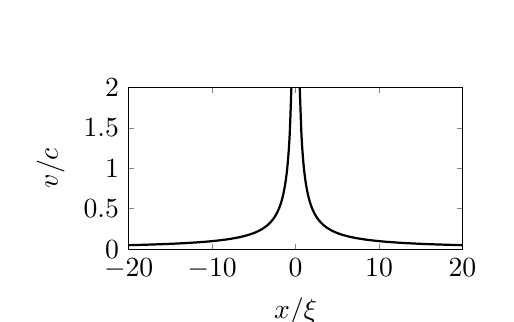
\begin{tikzpicture}
    \begin{axis}[
        width=0.48\linewidth,
        height=0.3\linewidth,
        xlabel=$x/\xi$,
        ylabel=$v/c$,
        xmin=-20,
        xmax=20.0,
        ymax=2,
        ymin=0,
        major tick length = 0.07cm
      ]
      \addplot[mark=none,color=black,thick,domain=0.5:20.0,smooth,samples=100] {1/sqrt(x*x)};
      \addplot[mark=none,color=black,thick,domain=-20.0:-0.5,smooth,samples=100] {1/sqrt(x*x)};
    \end{axis}
  \end{tikzpicture}
  \caption{(a) A comparison of the true vortex solution (black solid line) at $x=0$, found by numerically propagating the GPE in imaginary time, and the Pad\'e approximation (red dashed line) for a vortex core with a charge of $n=1$. (b) Fluid velocity in the vicinity of a vortex at $x=0$ with charge $n=1$.}\label{fig_vortex}
 \end{figure}

As seen in Section \ref{section:hydrodynamic}, the velocity of the fluid can be written $\mathbf{v} = \frac{h}{m}\nabla\theta$, where $\theta$ is the phase. We can use this with Equation \ref{eq_vortexsol} to find the velocity of the fluid around a vortex,
	\begin{equation}\label{eq_vortexvel}
	\mathbf{v}(\mathbf{r},\varphi) = \frac{n \hbar}{mr} {\bm{\hat{\varphi}}}.
	\end{equation}
Note the $v \propto 1/r$ dependence in the speed of the fluid around the vortex, demonstrated in Figure \ref{fig_vortex} (b). Once vortices are around $20\xi$ apart the velocity field is almost nil and the interaction between them is small.



\section{\label{section:inital} Initial Conditions}
	When numerically solving the GPE, an initial condition must be chosen. Correct choice of initial condition is important for accurate simulation of dynamics. If a unstable initial condition is chosen far from the ground state solution, noise and other excitations such as solitary waves and vortices may be generated that interfere with any measurements and studies undertaken at later times in the numerical computation. A selection of appropriate non-violent initial conditions are outlined in this section. 
	\subsection{\label{section:homoinit} Homogeneous initial condition}
	When the potential term $V=0$, the condensate ground state becomes homogeneous with density $\rho=\mu/g$. In this case, a stationary solution of the GPE is as simple as setting the ground state density everywhere,
	\begin{equation}
		\Psi = \sqrt{\frac{\mu}{g}}.
		\label{eq:homoinit}
	\end{equation}

	\subsection{\label{section:tftrap} Thomas-Fermi profile of a trapped condensate}
	Consider an initial condition that is stationary in time, but has a non-zero potential and so varies in space. Such a condition will necessarily satisfy \ref{eq:stationgpe}, the time-independent GPE. Let us assume that we have a strongly repulsive interaction term ($g>>0$). In this case, as an approximation we can neglect the kinetic energy term in the solution as it will be negligible compared to the strength of the repulsive atom-atom interactions. We write
	\begin{equation}
		\mu\Psi({\bf r}) = \left(V({\bf r}) + g|\Psi({\bf r})|^2  \right) \Psi({\bf r}),
	\end{equation}
	which can be simplified as,
	\begin{equation}
	 |\Psi({\bf r})|^2=\frac{\mu - V({\bf r})}{g}.
	\end{equation}
	From this result, we then construct an approximate solution,
	\begin{equation}
	\Psi({\bf r}) =
	\begin{cases} 
    \sqrt{\frac{\mu - V({\bf r})}{g}} & \mathrm{if}~\mu\geq V({\bf r}), \\
    0 & \mathrm{otherwise}.
  \end{cases}
  \end{equation}
	This is known as the Thomas-Fermi (TF) profile and is extremely useful as an approximate initial condition for modelling a trapped atomic condensate. The approximation is accurate near the centre of the condensate, but fails near the condensate edge, where the tails of the true density distribution are not captured. Nevertheless Figure \ref{fig_tfprofile} demonstrates the high accuracy of the approximation.
	\begin{figure}
	\centering
   \begin{tikzpicture}
    \begin{axis}[
        width=0.58\linewidth,
        height=0.3\linewidth,
        xlabel=$x/l_r$,
        ylabel=$|\phi|^2$,
        xmin=-20,
        xmax=20,
        ymin=0,
        major tick length = 0.07cm
      ]
      \addplot gnuplot [raw gnuplot,mark=none,color=black,thick]{
      	plot "numerics/figures/TF.dat" using 1:2 with lines;
      };
      \addplot gnuplot [raw gnuplot,mark=none,color=red,thick,dashed]{
      	plot "numerics/figures/TF.dat" using 1:3 with lines;
      };
    \end{axis}
  \end{tikzpicture}
  \begin{tikzpicture}
    \begin{axis}[
        width=0.38\linewidth,
        height=0.3\linewidth,
        xlabel=$x/l_r$,
        ylabel={},
        xmin=6,
        xmax=8.5,
        major tick length = 0.07cm
      ]
      \addplot gnuplot [raw gnuplot,mark=none,color=black,thick,smooth]{
      	plot "numerics/figures/TF.dat" using 1:2 with lines;
      };
      %\addplot gnuplot [raw gnuplot,mark=none,color=green,thick,dashed,samples=100]{
      	%plot "numerics/figures/TF.dat" using 1:3 with lines;
      %};
      \addplot[mark=none,color=red,dashed,thick,domain=6:7.11,smooth,samples=100] {(25.26698674-0.5*x*x)/2000.0};
      \addplot[mark=none,color=red,dashed,thick,domain=7.11:9,smooth,samples=100] {0.0*x};
    \end{axis}
  \end{tikzpicture}
  \caption{Comparison of the TF profile (red dashed line) and the true trapped harmonic oscillator ground state (black solid line) as found by numerical solution of the GPE in imaginary time. The TF profile fits extremely well over most of the condensate density (left), however fails at capturing the smooth tails of the density distribution (right). Here the TF radius is approximately $R_{\mathrm{TF}} = 7.1\,l_r$ and can be identified as a kink in the TF profile.}\label{fig_tfprofile}
 \end{figure}
 Due to the discrepancy at the tails of the condensate density, it is often the case that the TF profile is used as an initial guess for numerical eigensolvers, which then find a time-independent numerical solution to be used as the true initial condition.

 The TF solution provides a useful analytic approximation for the size of a condensate. The perimeter of the fluid occurs approximately when $\mu = V({\bf r})$, and so the approximate Thomas-Fermi radius of the condensate is,
	\begin{equation}
	R_{\mathrm{TF}} = \sqrt{\frac{2\mu}{m\omega_r^2}}.
	\end{equation}
Similarly to the size of a vortex core, the healing length, or box size in homogeneous systems, the TF radius is an useful indicator of length scales when working with analytical descriptions of condensate behaviours in a trapped system.

\subsection{\label{section:cfieldinit} Classical Field approximation with a homogeneous condensate}
	\begin{equation}
	\psi({\bf r},t) = \sum_{\bf k} a_{\bf k} \exp (\mathrm{i}{\bf k}\cdot{\bf r}),
	\label{eq:cFieldIC}
	\end{equation}
	where the complex Fourier amplitudes $a_{\bf k}$ are related to the occupation numbers $n_{\bf k}$ through $\braket{a_{\bf k}^{\,}a_{\bf k'}^*} = n_{\bf k}\delta_{\bf kk'}$. The phase of the complex amplitudes $a_{\bf k}$ are distributed uniformly on $[0,2\pi]$ while $|a_{\bf k}|$ is distributed randomly with fixed mean equal to unity; it has been found that different distributions of $|a_{\bf k}|$ make no qualitative difference to the turbulent evolution[phys rev A 66 013603]. [TODO: write about choice of E and N here to get different condensate fractions]

\section{\label{section:potentials}Creating obstacles with repulsive potentials}
In ultra-cold atomic gas experiments, perturbations to the gas can be achieved using laser beams. A red-detuned laser beam can create areas of attraction, and conversely, blue-detuned laser beams can create areas of repulsion. Should the blue-detuned laser beam be bright enough, a localised `hole' in the condensate can be formed where there are no atoms. Similarly, in superfluid helium experiments, there are examples where the fluid can feel the presence of a wall, wire, spheres or ion bubbles. These effects are replicated in the GPE model through the use of two and three-dimensional Gaussian or hard wall potentials.
\subsection{\label{section:3dobjpotential} Three-dimensional elliptical Gaussian}
In our 3D simulations, we solve the 3D GPE of Equation (1), where the localized obstacle is modelled via a repulsive ellipsoidal Gaussian potential,
\begin{equation}
V_{\mathrm{obj}}({\bf r})=V_0 \exp \left( -\frac{\varepsilon^2(x-x_0)^2}{d^2} -\frac{(y-y_0)^2}{d^2}-\frac{(z-z_0)^2}{d^2}\right),
\label{eq:potential3D}
\end{equation}
where  $V_0$ is its amplitude, $d$ its width in the $y$ and $z$ directions, and $(x_0,y_0,z_0)$ its coordinates. $\varepsilon$ parametrises the ellipticity of the obstacle, a value of $\varepsilon=1$ corresponds to a spherical obstacle, a higher value of $\varepsilon$ `squashes' the obstacle along $x$, forming a pancake shape.

\subsection{\label{section:3dcylinderpotential} Two and Three-dimensional cylindrical Gaussian}
A relatively simple experimentally realisable potential in quasi-2D and 3D quantum gas experiments is a hole (also referred to as a barrier or obstacle), generated by a blue-detuned laser beam. We model this potential as a Gaussian,
\begin{equation}
V_{\mathrm{obj}}({\bf r})=V_0 \exp \left( -\frac{\varepsilon^2(x-x_0)^2}{d^2} -\frac{(y-y_0)^2}{d^2}\right),
\end{equation}
where  $V_0$ is its amplitude, $d$ its width in the $y$ directions, and $(x_0,y_0,z_0)$ its coordinates. $\varepsilon$ parametrises the ellipticity of the Gaussian (experimentally feasible with laser beam focusing or masking), so that a value of $\varepsilon=1$ corresponds to a circular shaped hole. In 3D the Gaussian hole is extended across the entire $z$ dimension forming a cylindrical shaped barrier.
\subsection{\label{section:3dafmpotential} Three-dimensional `realistic' rough-surface}
\begin{figure}
	\centering
   \begin{tikzpicture}
    \begin{axis}[view={0}{90},
        width=0.5\linewidth,
        height=0.5\linewidth,
        xlabel=$x/\mu m$,
        ylabel=$y/\mu m$,
        xmin = 0,
        xmax = 1,
        ymin = 0,
        ymax = 1,
        major tick length = 0.07cm,
        colorbar style={title={$z/nm$},text width=0.5em,major tick length = 0.07cm},
		    major tick length = 0.07cm,
		    point meta min = 1.5,
		    point meta max = 5.5,
		    colorbar,colormap={pm3d}{rgb=(0,0,0);
                              rgb=(0.5,0.125,1);
                              rgb=(0.707,0.125,0);
                              rgb=(0.866,0.422,0);
                              rgb=(1,1,0)}
      ]
      \addplot graphics [xmin=0,xmax=1,ymin=0,ymax=1] {numerics/figures/afm_surf.png};
    \end{axis}
  \end{tikzpicture}
  \caption{An atomic force microscope (AFM) image showing the microscopic detail on the surface of a  single--core NbTi `floppy' wire used for generating superfluid turbulence. This data was kindly provided by C. R. Lawson \cite{Lawson}.}\label{fig_afmprofile}
 \end{figure}

In many superfluid helium experiments \cite{VinenSkrbek2008}, turbulence
is generated by moving grids \cite{Davis2000},
wires \cite{Guenault1986,brad05,Bradley2011,Fisher2001,goto08},
forks \cite{Blaauwgeers2007,Bradley2012} or spheres \cite{Schoepe1995}.
Although macroscopically polished, the surface of these objects is
rough on the length scale of the superfluid vortex core, which is of
the order of $10^{-10}~\rm m$ in $^4$He
and $10^{-8}~\rm m$ in $^3$He.  As an example, Fig.~\ref{fig_afmprofile}(a) is an atomic force microscope (AFM) image showing the microscopic detail on the surface of a  single--core NbTi `floppy' wire used for generating superfluid turbulence  \cite{Bradley2011}.  Note the appearance of an elongated scratch, typical of such wires.  No direct flow visualization is available on these microscopic length scales and, as such, 
superflow in the presence of walls remains poorly understood. In principle, the superfluid boundary conditions should
be straightforward.
In the simplest case of a boundary at rest, the superfluid velocity
component which is perpendicular to the boundary must be equal to
zero at the boundary, while the tangential component can slip.
In practice, nucleation of quantum vorticity complicates
this idealized Eulerian picture. We can simulate the microscopic detail in GPE models through the use of a potential derived from the sample AFM height-map data. We define the external potential to be,
\begin{equation}
V_{\mathrm{obj}}({\bf r}) =
\begin{cases}
V_0 &\mbox{if } z < (h(\alpha x,\alpha y)-z_0)  \\
0 &\mbox{if } z > (h(\alpha x,\alpha y)-z_0),
\end{cases}
\label{eq:potentialAFM3D}
\end{equation}
where $V_0$ is its amplitude, $z_0$ is a shift in height and $\alpha$ is a scaling factor. Scaling $h(x,y)$ acts as a crude way of varying 
the roughness of simulated boundaries. Finally, a Gaussian blur is applied so that $V(x,y,z)$ is smooth in $z$.

%\subsection{\label{section:2dbitmappotential} Two-dimensional arbitrary bitmap}
%\begin{equation}
%V({\bf r})=
%	\begin{cases} 
%    V_0 & \mathrm{if}~ \text{the pixel at (x,y) is white}, \\
%    0   & \mathrm{if}~ \text{the pixel at (x,y) is black},
%  \end{cases}
%\end{equation}
%where $V_0$ is its amplitude.

\end{chapter}

  \begin{chapter}{\label{cha:numerics}Numerical Theory and Procedures}
\section{\label{section:RK} Numerical procedures for 2D and 3D solutions}
	\subsection{\label{section:RK4} Fourth order Runge-Kutta scheme}
	The classical fourth-order Runge-Kutta formula (RK4) is described equivalently in many texts. We follow the description in \cite{NumericalRecipes}. Let an initial value problem be specified as
	
	\begin{align*}
		\frac{\partial \psi}{\partial t} &= f(\psi,t),\hspace{0.25in}\psi(t_0) = \psi_0.
	\end{align*}

A step-size, $h>0$, is chosen as the parameter controlling how the solution is advanced over $t$. The scheme for estimating $\psi(t_n)= \psi_n$ is then written
\begin{equation}
\begin{split}
		k_1 &= hf(t_n,\psi_n),\\
		k_2 &= hf(t_n+\frac{h}{2},\psi_n+\frac{k_1}{2}),\\
		k_3 &= hf(t_n+\frac{h}{2},\psi_n+\frac{k_2}{2}),\\
		k_4 &= hf(t_n+h,\psi_n+k_3),\\
		\psi_{n+1} &= \psi_n + \frac{k_1}{6}+ \frac{k_2}{3}+ \frac{k_3}{3} + \frac{k_4}{6} + \mathcal{O}(h^5),\\
		t_{n+1}  &= t_n + h.
		\label{eq:rk4}
\end{split}
\end{equation}


	An outline derivation of the Runge-Kutta scheme, which includes a proof of accuracy are shown in Appendix \ref{appsection:rk4deriv}.
	In all of our relevant calculations the value of f is set as the right hand side of the homogeneous or trapped GPE. The main loop formulating the RK4 method may be repeated indefinitely to reach any $t>t_0$. The step size for a given set of parameters should be chosen small enough that smaller choices make no quantitative changes to the resulting solution. The following section outlines the methods we have implemented to ensure numerical solutions are converged.

	\subsection{\label{section:numericalParams} Numerical stability and convergence}
	We now investigate numerical parameters which affect the stability of simulated superfluid systems. Our direct aim is to find a suitable discretisaton of space and time so that while simulations are timely, our numerical quantities are converged (so that they are not sensitive to small changes in computational parameters) and that quantities conserved by the equations of motion are indeed conserved in the computed numerical solutions.

	We begin by estimating $\Delta_x$, the required spatial grid spacing, by considering the width of the vortex core in a homogeneous system, a feature we would like well and accurately visualised in our numerical solutions. Through observation of a singly quantised vortex core (as in Figure \ref{fig_vortex}) we observe a core radius of approximately $5\xi$ when the background density is $\rho=1$. To ensure the vortex core structure is well resolved we decide to dedicate 10 grid points for a vortex core radius, suggesting a value of $\Delta_x = \xi/2$.

	In the trapped case we can use the same idea. It is shown in Section \ref{section:healing} that $\xi = \hbar/\sqrt{mg}$ for $\rho=1$. We can then easily rearrange to find an expression for $\xi$ in the harmonic oscillator units of trapped condensates. We find that our approximate grid spacing to adequately resolve the vortex core is $\Delta_x = 0.5\xi = 0.5\omega \sqrt{\hbar/(\mu \omega)} l_r$. As an example, for a trapped condensate with interaction energy $\hat{g}=2000$, chemical potential $\hat{\mu}=25.27$ and trap frequency $\omega=8.75~{\rm Hz}$ we find that a value of $\Delta_x=0.1l_r$ should be adequate. 

	Similar arguments (concerned with time rather than space), can be used to approximate a suitable time step $h$. We define a time period that we would like to be well resolved by considering by the smallest possible element moving at the fastest reasonable speed. If we define this period as $\Delta_x / 5~c$ and allocate to it 10 time steps, we find that $h = 0.5\xi/50~c = 0.01\tau$.

  In addition to this process, for each set of simulation parameters it is recommended to confirm the suitability of the chosen $\Delta_x$ and $h$ by testing the convergence and conservation in the numerical methods. The total condensate energy and particle number are good measures for this as they should both be well conserved by the GPE with a dissipation of $\gamma=0$. An example of this process (confirming the suitability of a chosen $\Delta_x$) is shown in Figure \ref{fig_energ_norm_cons}: For a large $\Delta_x=0.4l_r$ both the condensate energy and norm fluctuate wildly. For $\Delta_x=0.1l_r$ the norm is extremely well conserved to within $2.10^{-5}\%$ and the energy is conserved within $5.10^{-3}\%$. The smallest tested value of $\Delta_x=0.05l_r$ finally confirms that the energy has converged. We conclude that for the chosen system parameters that $\Delta_x=0.1l_r$ (the value suggested by the above analysis) is numerically sufficient and there is little reason to use $\Delta_x<0.1l_r$.

  \begin{figure}
  \centering
   \begin{tikzpicture}
    \begin{axis}[y tick label style={
            /pgf/number format/.cd,
                fixed,
                fixed zerofill,
                precision=3,
            /tikz/.cd
        },
        width=0.98\linewidth,
        height=0.3\linewidth,
        xlabel={},
        ylabel=$\hat{E}\left ( \hat{t} \right )$,
        xmin=0,
        xmax=10,
        major tick length = 0.07cm
      ]
      \addplot gnuplot [raw gnuplot,mark=none,color=black,thick]{
        plot "numerics/figures/energ-norm-cons.0.05" using 1:3 with lines;
      };
      \addplot gnuplot [raw gnuplot,mark=none,color=red,thick]{
        plot "numerics/figures/energ-norm-cons.0.1" using 1:3 with lines;
      };
      \addplot gnuplot [raw gnuplot,mark=none,color=green,thick]{
        plot "numerics/figures/energ-norm-cons.0.2" using 1:3 with lines;
      };
      \addplot gnuplot [raw gnuplot,mark=none,color=blue,thick]{
        plot "numerics/figures/energ-norm-cons.0.4" using 1:3 with lines;
      };
    \end{axis}
  \end{tikzpicture}
  \begin{tikzpicture}
    \begin{axis}[y tick label style={
            /pgf/number format/.cd,
                fixed,
                fixed zerofill,
                precision=4,
            /tikz/.cd
        },
        width=0.98\linewidth,
        height=0.35\linewidth,
        name=mainplot,
        xlabel=$\hat{t}$,
        ylabel=$\hat{N}\left ( \hat{t} \right )$,
        xmin=0,
        xmax=10,
        ymax=1.0008,
        major tick length = 0.07cm
      ]
      \addplot gnuplot [raw gnuplot,mark=none,color=black,thick]{
        plot "numerics/figures/energ-norm-cons.0.05" using 1:4 with lines;
      };
      \addplot gnuplot [raw gnuplot,mark=none,color=red,thick]{
        plot "numerics/figures/energ-norm-cons.0.1" using 1:4 with lines;
      };
      \addplot gnuplot [raw gnuplot,mark=none,color=green,thick]{
        plot "numerics/figures/energ-norm-cons.0.2" using 1:4 with lines;
      };
      \addplot gnuplot [raw gnuplot,mark=none,color=blue,thick]{
        plot "numerics/figures/energ-norm-cons.0.4" using 1:4 with lines;
      };
      \node[anchor=west] (source) at (axis cs:9.25,1.00027){};
      \node[anchor=west] (destination) at (axis cs:9.25,1.0000){};
      \node[anchor=west] (topl) at (axis cs:9.2,1.00005){};
      \node[anchor=west] (botr) at (axis cs:9.8,0.99995){};
      \draw[->](source)--(destination);
      \draw(topl) rectangle (botr);
    \end{axis}
    \begin{axis}[y tick label style={
            /pgf/number format/.cd,
                fixed,
                fixed zerofill,
                precision=6,
            /tikz/.cd
        },
        width=0.35\linewidth,
        height=0.18\linewidth,
        at={(mainplot.north east)},anchor=north east,
        xlabel={},
        ylabel={},
        xmin=9.15,
        xmax=9.85,
        major tick length = 0.07cm
      ]
      \addplot gnuplot [raw gnuplot,mark=none,color=black,thick]{
        plot "numerics/figures/energ-norm-cons.0.05" using 1:4 with lines;
      };
      \addplot gnuplot [raw gnuplot,mark=none,color=red,thick]{
        plot "numerics/figures/energ-norm-cons.0.1" using 1:4 with lines;
      };
      \addplot gnuplot [raw gnuplot,mark=none,color=green,thick]{
        plot "numerics/figures/energ-norm-cons.0.2" using 1:4 with lines;
      };
    \end{axis}
  \end{tikzpicture}
  \caption{Dimensionless energy, $\hat{E}$, and particle number, $\hat{N}$, throughout numerical propagation of a trapped condensate containing a singly quantised vortex in its center, with interaction energy $\hat{g}=2000$ and chemical potential $\hat{\mu}=25.27$. The numerical grid width varies with each line; $\Delta_x = 0.05$ (black), $\Delta_x = 0.1$ (red), $\Delta_x = 0.2$ (green) and $\Delta_x = 0.4$ (blue). (Inset) Zoomed view of the $\hat{N}$.}\label{fig_energ_norm_cons}
 \end{figure}

\section{\label{section:vortexidentifying} Identifying vortices}
Large potions of this thesis are dedicated to the study of 2D vortex dynamics. As such, accurate detection of the location and charge of densely packed quantised 2D vortices is required, and so we have developed robust numerical methods for vortex identification. The basic idea is fairly simple, with arguments similar to those used to demonstrate the quantised nature of the circulation.

As shown in Section \ref{section:quantisedcirculation}, the integrated change of phase along any closed curve $C$ is,
\begin{equation}
  \Delta\theta(C) = \oint_C \! \nabla \theta  \, \mathrm{d}\mathbf{l} = 2\pi q,
\end{equation}
where $\mathrm{d}\mathbf{l}$ is the line element and $q\in\mathbb{Z}$. Further, the fundamental theorem of calculus for line integrals[CITE] implies that $\Delta\theta(C) = 0$, providing that $C$ is continuous and does not encompass a phase singularity. This result is crucial; it allows us to directly state that a vortex lies within $C$ if and only if $|\Delta\theta(C)| > 0 $.

\subsection{\label{section:vortexloc} Basic vortex detection method}
First define a set of curves $C_k$ with each curve lying on points of our numerical grid, so that a single $C_k$ encompasses only a small region of the fluid (ideally, $C_k$ should encompass a region at most the diameter of a vortex core). $\Delta\theta(C_k)$ is then approximated for each $k$ using numerical differentiation (2nd order finite differences) and numerical line integration (trapezium or Simpson rule). If $\Delta\theta(C_k) = 0$ to within numerical accuracy then we determine that the region inside $C_k$ contains no vortices. Otherwise the sign of $\Delta\theta(C_k)$ tells us the polarity of the encompassed vortex.

In principle the result also allows us to calculate the exact charge of a vortex in terms of the quantum of circulation. However, for accurate determination of vortex location the curves $C_k$ must encompass a very small area, contain few grid points, and so accuracy is low. We use only the sign of the $\Delta\theta(C_k)$ so that the integration error makes minimal difference and results in an accurate detection of vortex polarity and location. As multiply charged ($|q|>1$) vortices are unstable (rapidly decaying into several singly charged vortices) there is no significant loss of information in practise.
\begin{figure}
  \centering
   \begin{tikzpicture}[
        %>={Straight Barb[left]},
      myarrow/.style={
        decoration={
          markings,
          mark=at position 0.5 with {\arrow{>}};
          },
        postaction=decorate  
        }
      ]
      \begin{axis}[
        xlabel={$x/\xi$},
        ylabel={$y/\xi$},
        x=1cm/4,
        y=1cm/4,
        xmin=-10,
        xmax=10,
        ymin=-10,
        ymax=10,
        colorbar style={title={Phase},text width=0.5em,major tick length = 0.07cm},
        major tick length = 0.07cm,
        point meta min = -3.1415,
        point meta max = 3.1415,
        colorbar,colormap name=hsvcl
      ]
      \addplot graphics [xmin=-10,xmax=10,ymin=-10,ymax=10] {numerics/figures/vortex1dp-hsv.png};
    \end{axis}
      \draw[step=1cm,gray,very thin] (0,0) grid (5,5);
      \foreach \i in {1,...,5}{
        \foreach \j in {1,...,5}{
          \draw [myarrow,thick] (\i-0.07,5.93-\j)--(\i-0.93,5.93-\j);
          \draw [thick] (\i-0.93,5.93-\j)--(\i-0.93,5.07-\j);
          \draw [thick] (\i-0.93,5.07-\j)--(\i-0.07,5.07-\j);
          \draw [thick] (\i-0.07,5.03-\j)--(\i-0.07,5.93-\j);
          {\pgfmathtruncatemacro{\label}{((\j-1)*5) + \i}
          \node[] (c0) at (\i-0.5,5.5-\j) {$C_{\label}$};}
        }
      }
  \end{tikzpicture}
  \caption{The phase for a homogeneous system with a vortex located at (0,0). Also shown is an example set of curves $C_k$ for vortex identification. All $\Delta\theta(C_{k\neq13})\approx0$, and $\Delta\theta(C_{13})>0$. The conclusion is that a positive vortex lies in the region defined by $C_{13}$.}
 \end{figure}
\subsection{\label{section:vortexloc} Visualising vortex location with a vortex field}
The basic vortex identification method set out in Section \ref{section:vortexloc} is quick to implement and useful when there are few well separated vortices, but one can easily imagine a situation where the system fails. One such case would be two vortices both lying within a single $C_k$ curve; in the case of two similarly charged vortices only a single vortex would be detected or in the case of two oppositely charged vortices potentially none at all!

The solution is not always as simple as reducing the size of $C_k$, vortices can be densely packed and there are often too little grid points to make this reasonable. Instead, curves with a width around the diameter of a vortex core are again used, but for every grid point (taking into account boundary conditions) the curve $C_{[i,j]}$ is defined surrounding and centred on the grid point $[i,j]$. A vortex field can then be visualised by visualizing the 2D plot of $\Delta\theta(C_{[i,j]})$. Algorithm \ref{algo_calcvortexfield} describes the process in detail. As before, areas where $|\Delta\theta(C_{[i,j]})| > 0$ (to within numerical accuracy) signify the presence of a vortex. Figure \ref{fig:vortexfield} demonstrates a vortex field obtained from a homogeneous system with a negative vortex located at $(-\xi,0)$ and a positive vortex located at $(\xi,0)$. It can be easily seen where the two vortices are located in the wavefunction by direct observation of the 2D vortex field.
\begin{figure}
  \centering
   \begin{tikzpicture}
      \begin{axis}[
        xlabel={$x/\xi$},
        ylabel={$y/\xi$},
        width=0.45\linewidth,
        height=0.45\linewidth,
        xmin=-10,
        xmax=10,
        ymin=-10,
        ymax=10,
        colorbar style={title={Vortex Field},text width=0.5em,major tick length = 0.07cm},
        major tick length = 0.07cm,
        point meta min = -6,
        point meta max = 6,
        colorbar,colormap/jet
      ]
      \addplot graphics [xmin=-10,xmax=10,ymin=-10,ymax=10] {numerics/figures/v-av-pair-vortexfield.png};
      \addplot[mark=.] coordinates {(-1,0)} node[pin={[pin edge={black,thick}]left:{$1$}}]{} ;
      \addplot[mark=.] coordinates {(1,0)} node[pin={[pin edge={black,thick}]right:{$2$}}]{} ;
    \end{axis}
    
  \end{tikzpicture}
  \caption{Vortex field for two oppositely charged vortices located at ($-\xi$,0) and ($\xi$,0) in a homogeneous system. The positive (negative) vortex leads to a positive (negative) quantity in the vortex field. In addition, the output of the bwlabel algorithm is labelled.\label{fig:vortexfield}}
 \end{figure}

For every vortex detected by this algorithm, the corresponding area in the vortex field is composed of several adjoined points in the numerical grid. For correct vortex counting, these multiple points must be classified as a single vortex. The bwlabel algorithm described in Algorithm \ref{algo_bwlabel} is used to obtain this required classification. The algorithm takes the vortex field as input and assigns each connected component a label. An example output of bwlabel is shown in Figure \ref{fig:vortexfield}. To find the vortex location for a given label, we simply take the mean of all the $x$ and $y$ locations of points with the same label.

The algorithm described in this section leads to more accurate vortex counts when vortices are densely packed. As a bonus the accuracy of detected vortex location is improved; the final output is a combination of information from several curves $C_{[i,j]}$, and so in good conditions the result is often sub-pixel accurate (that is, the algorithm output is accurate even if the phase singularity corresponding to a vortex lies between grid points). 

\subsection{\label{section:gaussianblur} Further improving accuracy with a Gaussian blur}
When using Algorithm \ref{algo_calcvortexfield} in `messy' wavefunctions (containing many vortices and waves), artefacts of the incorrect sign can be introduced by the numerical discretisation, differentiation and integration errors. Faint examples of these artefacts can be seen in Figure \ref{fig:vortexfield} surrounding the two labelled regions. These artefacts are spatially small (on the scale of $\Delta_x$) and so can be corrected by removing all high frequency spatial waves from the vortex field using low-pass filtering. A common low-pass filter is the Gaussian blur [CITE], applied using a convolution. The Gaussian blur algorithm is described in Algorithm \ref{algo_gaussconv} and the result of applying the algorithm to he vortex field is shown in Figure \ref{fig:vortexfieldsmooth}. Note how the incorrectly signed artefacts surrounding the detected vortex regions are now removed.
\begin{figure}[!ht]
  \centering
   \begin{tikzpicture}
      \begin{axis}[
        xlabel={$x/\xi$},
        ylabel={$y/\xi$},
        width=0.45\linewidth,
        height=0.45\linewidth,
        xmin=-10,
        xmax=10,
        ymin=-10,
        ymax=10,
        colorbar style={title={Vortex Field},text width=0.5em,major tick length = 0.07cm},
        major tick length = 0.07cm,
        point meta min = -5.1,
        point meta max = 5.1,
        colorbar,colormap/jet
      ]
      \addplot graphics [xmin=-10,xmax=10,ymin=-10,ymax=10] {numerics/figures/v-av-pair-vortexfield-smoothed.png};
    \end{axis}
  \end{tikzpicture}
  \caption{Smoothed vortex field for two oppositely charged vortices located at ($-\xi$,0) and ($\xi$,0) in a homogeneous system. The high frequency noisy artefacts in the vortex field are removed by the low-pass filtering.\label{fig:vortexfieldsmooth} }
 \end{figure}

 A by-product of applying a low-pass filter to the vortex field is that sharp edges in structures are blurred and spread out. To identify vortex locations a threshold function is therefore used before performing the bwlabel algorithm, i.e vortices are identified when $|\Delta\theta(C_{[i,j]})| > \Delta_{\rm th}$, where $\Delta_{\rm th}>0$ is some threshold. $\Delta_{\rm th}$ can be tweaked to make the vortex detection more or less sensitive (for either detecting vortices more easily in messy systems, or to ignore weak spurious signals in the vortex field) and in general will vary for each system.
\subsection{\label{section:ghostvortex} Avoiding `ghost vortices'}
A common problem when detecting vortices is the prevalence of invalid or uninteresting phase defects inside obstacles or when considering trapped condensates. In areas where the density is exactly zero the system phase becomes undefined. Depending on how the simulation is implemented these areas may fill with small numerical noise and cause many singularities to be detected. A similar phenomenon occurs in areas of near-zero density; well-defined singularities in the phase form but with an ill-defined vortex core in the density \cite{tsubota_kasamatsu_02}. Examples of these vortices are shown in the low density regions of Figure \ref{fig:ghostvortex}. As these singularities carry negligible angular momentum and energy they are of no interest and are termed `ghost vortices'.
\begin{figure}[!ht]
  \centering
   \begin{tikzpicture}
      \begin{axis}[
        xlabel={$x/l_r$},
        ylabel={$y/l_r$},
        width=0.44\linewidth,
        height=0.44\linewidth,
        xmin=-25,
        xmax=25,
        ymin=-25,
        ymax=25,
        major tick length = 0.07cm
      ]
      \addplot graphics [xmin=-25,xmax=25,ymin=-25,ymax=25] {numerics/figures/vortexlatticedens.png};
    \end{axis}
  \end{tikzpicture}
  \begin{tikzpicture}
      \begin{axis}[
        xlabel={$x/l_r$},
        ylabel={},
        width=0.44\linewidth,
        height=0.44\linewidth,
        xmin=-25,
        xmax=25,
        ymin=-25,
        ymax=25,
        colorbar style={title={Phase},text width=0.5em,major tick length = 0.07cm},
        major tick length = 0.07cm,
        point meta min = -3.141592,
        point meta max = 3.141592,
        colorbar,colormap name=hsvcl
      ]
      \addplot graphics [xmin=-25,xmax=25,ymin=-25,ymax=25] {numerics/figures/vortexlatticephase.png};
    \end{axis}
  \end{tikzpicture}
  \caption{A trapped rotating condensate with $\Omega=0.7$, $\hat{g}=2000$ and $\hat{\mu}=25.27$. Ghost vortices can be seen in the phase as singularities where the corresponding density is near-zero.\label{fig:ghostvortex}}
 \end{figure}

A simple way to remove ghost vortices is to use a mask to hide vortices found in low-density regions in trapped systems and inside obstacles. While on the one hand it is easy to define a mask using the TF radius or considering where $V_{\rm trap} + V_{\rm obj}>1$, masks are quite arbitrary in nature and an overzealous mask may hide details. Additionally, any condensate with certain excitations such a breathing mode or centre of mass oscillation will periodically extend beyond a hard coded mask.

An alternative method to avoid identifying ghost vortices presents itself when implementing Algorithm \ref{algo_calcvortexfield}. The vortex field can be multiplied by the wavefunction density at every point {\it before} performing the Gaussian convolution step. The result is that in low-density areas the vortex field becomes completely zero and singularities in this region are no longer identified as vortices. At the centre of vortex cores the vortex field also goes to zero. However, enough vortex information remains in the vortex field in the vicinity of the vortex cores that vortices in high-density regions are still identified accurately after the Gaussian convolution. As before, the threshold value $\Delta_{\rm th}$ controls the sensitivity of this algorithm, in particular for detecting vortices in the low density regions of the condensate. Algorithm \ref{algo_calcvortexfielddens} describes this method in further detail and Figure \ref{fig:filtervortexlattice} shows the vortex field with and without the added step of multiplying by the density, demonstrating that the ghost vortices detected when using Algorithm \ref{algo_calcvortexfield} are indeed removed when using Algorithm \ref{algo_calcvortexfielddens}.
\begin{figure}[!ht]
\begin{center}
\begin{minipage}{0.8\linewidth}%
   \begin{tikzpicture}
      \begin{axis}[
        xlabel={},
        ylabel={$y/l_r$},
        width=0.5\linewidth,
        height=0.5\linewidth,
        xmin=-25,
        xmax=25,
        ymin=-25,
        ymax=25,
        major tick length = 0.07cm
      ]
      \addplot graphics [xmin=-25,xmax=25,ymin=-25,ymax=25] {numerics/figures/vortexlattice-vortexfield.png};
    \end{axis}
  \end{tikzpicture}%
  \begin{tikzpicture}
      \begin{axis}[
        xlabel={},
        ylabel={},
        width=0.5\linewidth,
        height=0.5\linewidth,
        xmin=-25,
        xmax=25,
        ymin=-25,
        ymax=25,
        colorbar style={title={Vortex Field},text width=0.5em,major tick length = 0.07cm},
        major tick length = 0.07cm,
        point meta min = -5.1,
        point meta max = 5.1,
        colorbar,colormap/jet
      ]
      \addplot graphics [xmin=-25,xmax=25,ymin=-25,ymax=25] {numerics/figures/vortexlattice-vortexfield-corrected.png};
    \end{axis}
  \end{tikzpicture}\\\vspace{1cm}%
  \begin{tikzpicture}
      \begin{axis}[
        xlabel={$x/l_r$},
        ylabel={$y/l_r$},
        width=0.5\linewidth,
        height=0.5\linewidth,
        xmin=-25,
        xmax=25,
        ymin=-25,
        ymax=25,
        major tick length = 0.07cm
      ]
      \addplot graphics [xmin=-25,xmax=25,ymin=-25,ymax=25] {numerics/figures/vortexlatticedens-withGvortex.png};
    \end{axis}
  \end{tikzpicture}%
  \begin{tikzpicture}
      \begin{axis}[
        xlabel={$x/l_r$},
        ylabel={},
        width=0.5\linewidth,
        height=0.5\linewidth,
        xmin=-25,
        xmax=25,
        ymin=-25,
        ymax=25,
        major tick length = 0.07cm
      ]
      \addplot graphics [xmin=-25,xmax=25,ymin=-25,ymax=25] {numerics/figures/vortexlatticedens-withvortex.png};
    \end{axis}
  \end{tikzpicture}%
\end{minipage}%
\end{center}
  \caption{Identifying vortices within a trapped rotating condensate with $\Omega=0.7$, $\hat{g}=2000$ and $\hat{\mu}=25.27$. (a) The smoothed vortex field using Algorithm \ref{algo_calcvortexfield}, (b) the smoothed vortex field using Algorithm \ref{algo_calcvortexfielddens}, (c) the system density with vortices identified using Algorithm \ref{algo_calcvortexfield}, and (d) the system density with vortices identified using Algorithm \ref{algo_calcvortexfielddens}. The ghost vortices seen in (a,c) are removed in (b,d).\label{fig:filtervortexlattice}}
 \end{figure}

\section{\label{section:vortexclustering} Quantifying vortex clustering in 2D}
With the ability to detect vortex polarity and locations in 2D, we can begin to better understand vortex distribution and statistics in simulations. In this section we describe the various methods of quantifying vortex distribution, both simple and complex.
  \subsection{\label{section:vortexcounting} Vortex counting}
  The simplest method of ascertaining vortex statistics is to simply count the number of vortices, $N_v$, in the entire system. A further obvious decomposition of this quantity is to count the number of positive and negative vortices separately, designated $N_+$ and $N_-$ respectively. With this information we can define an interesting property of a system's vortex distribution,
  \begin{equation}
    P_v = \frac{N_+ - N_-}{N_v},
  \end{equation}
  where $P_v$ is known as the polarity of the system. This quantity takes values in the range $[-1,1]$; when there are only positively (negatively) charged vortices in the system $P_v=1$ ($P_v=-1$), and when there are equal quantities of positive and negatively charged vortices $P_v=0$.
  \subsection{\label{section:ripleysk} Ripley's $K$ and $L$ functions }
  While counting vortices as in Section \ref{section:vortexcounting} is a great way to gain statistics of the distribution of vortices in terms of vortex charge, the quantities tell us nothing about how vortices are located in space. The problem of spatial descriptive statistics is an old one and measures of spatial dispersion or homogeneity have in the past been applied to several datasets consisting of point locations, very similar to the results of our vortex detection algorithms. Some of these applications include spatial distribution of trees \cite{duncan_1993,peterson_1995,stoyan_2000}, plants \cite{stamp_1990}, bird nests \cite{gaines_2000} and the spread of disease \cite{diggle_1991}.


  One such measure of homogeneity is Ripley's $K$ Function \cite{dixon_2002}, defined theoretically in the following way,
  \begin{equation}\label{eq:ripleysktheory}
    K(s) = \lambda^{-1}E[\text{\# of points within distance $s$ of a randomly chosen point}],
  \end{equation}
  where $\lambda$ is the density (number per unit area) of points. $K(s)$ can be analytically evaluated when it is known that points are distributed according to a homogeneous Poisson process, i.e. randomly placed in space. In this case each point is independent from all the other points and the resulting equation for $K(s)$ is known as complete spatial randomness (CSR),
  \begin{equation}\label{eq:ripleyskcsr}
    K(s) = \pi s^2.
  \end{equation}
  The simplest use of Ripley's $K$ function is to approximate $K(s)$ from an observed set of points and test the result of CSR. Should the result be inconsistent with CSR, $K(s)$ can also tell us at what length scales the points deviate from spatial homogeneity.

  For most of our simulations, $K(s)$ can be easily estimated by using observed vortex locations.
  \begin{equation}\label{eq:ripleysk}
    \hat{K}(s) = \frac{A}{N_v^2}\sum\limits_{i}\sum\limits_{j \ne i} I\left (d_{ij}<s\right ),
  \end{equation}
  where $d_{ij}$ is the distance between the $i$th and $j$th vortex, $A$ is the area of the region of interest, $N_v$ is the number of vortices, and I is the indicator function (1 if its argument is true, 0 otherwise). In homogeneous simulations $A$ could be as simple as the numerical box area, while with a trapped condensate calculating $A$ could involve measuring the bulk part of the condensate or calculating an area using the TF radius.

  Equation \ref{eq:ripleysk} ignores so called {\it edge effects}. These effects arise when the search radius $s$ becomes large enough that the lack of points outside the region of interest begins to bias the estimator $\hat{K}(s)$. Ripley provides an edge-corrected estimator \cite{ripley_1976} which takes the form,
  \begin{equation}\label{eq:ripleyskedge}
    \hat{K}(s) = \frac{A}{N_v^2}\sum\limits_{i}\sum\limits_{j \ne i} w({\bf r}_i,{\bf r}_j)^{-1}I\left (d_{ij}<s\right ),
  \end{equation}
  where the weight function, $w({\bf r}_i,{\bf r}_j)$, provides edge correction. If the circle centred on  the point ${\bf r}_i$ and passing through the point ${\bf r}_j$ completely lies within the region of interest, then $w({\bf r}_i,{\bf r}_j)=1$, otherwise $w({\bf r}_i,{\bf r}_j)$ is equal to the proportion of the circumference of the circle that is inside the region of interest. The edge-corrected estimator provided by Equation \ref{eq:ripleyskedge} should be used when we are interested in large spatial scale homogeneity, i.e. when $s$ is large, as it is on this scale edge-effects can dominate.

  Visualising $\hat{K}(s)$ can be made easier by considering Ripley's $L$ function, with estimator,
  \begin{equation}\label{eq:ripleysl}
    \hat{L}(s) = \sqrt{\frac{\hat{K}(s)}{\pi}}.
  \end{equation}
  $L(s)$ has the useful properties that under CSR the variance is approximately constant \cite{ripley_1979}, which can be used as a secondary check, and $L(s) - s$ should be approximately zero for all $s$. Deviations from zero allows us to immediately identify in what way, as well as at what scale, spatial homogeneity is broken in the dataset.
\begin{figure}[!ht]
  \begin{minipage}{0.5\linewidth}%
  \begin{tikzpicture}[domain=-5:5]
    \begin{axis}[xlabel={$x$}, ylabel={$y$},
        xmin=-5.05,
        xmax=5.05,
        ymin=-5.05,
        ymax=5.05,
        major tick length = 0.07cm,
        width=\linewidth,
        height=\linewidth,
        scatter/classes={ 0={mark=*,blue}},
        mark size = 0.7
        ]
    \addplot[scatter, only marks, scatter src=\thisrow{class},
          error bars/.cd, y dir=both, x dir=both, y explicit, x explicit]
          table[x=x,y=y] {numerics/figures/ripleypoints.dat};
    \end{axis}
  \end{tikzpicture}%
  \end{minipage}%
  \begin{minipage}{0.5\linewidth}%
  \begin{tikzpicture}
    \begin{axis}[y tick label style={
            /pgf/number format/.cd,
                fixed,
                fixed zerofill,
                precision=0,
            /tikz/.cd
        },
        width=\linewidth,
        height=0.53\linewidth,
        xlabel={s},
        ylabel=$\hat{K}(s)$,
        xmin=0,
        xmax=4,
        major tick length = 0.07cm
      ]
      \addplot gnuplot [raw gnuplot,mark=none,color=black,thick]{
        plot "numerics/figures/ripleyKpoints.dat" using 1:2 with lines;
      };
      \addplot gnuplot [raw gnuplot,mark=none,color=black,dashed,thick]{
        plot "numerics/figures/ripleyKpoints.dat" using 1:(3.141592*$1*$1) with lines;
      };
    \end{axis}
  \end{tikzpicture}\\%
  \begin{tikzpicture}
    \begin{axis}[y tick label style={
            /pgf/number format/.cd,
                fixed,
                fixed zerofill,
                precision=0,
            /tikz/.cd
        },
        width=\linewidth,
        height=0.53\linewidth,
        xlabel={s},
        ylabel=$\hat{L}(s)-s$,
        xmin=0,
        xmax=4,
        major tick length = 0.07cm
      ]
      \addplot gnuplot [raw gnuplot,mark=none,color=black,thick]{
        plot "numerics/figures/ripleyKpoints.dat" using 1:(sqrt($2/3.1415926)-$1) with lines;
      };
      \addplot gnuplot [raw gnuplot,mark=none,color=black,dashed,thick]{
        plot "numerics/figures/ripleyKpoints.dat" using 1:(0*$1*$1) with lines;
      };
    \end{axis}
  \end{tikzpicture}%
  \end{minipage}%
  \caption{Sample points (left) used for estimating Ripley's $K$ and $L$ functions. Shown (right) are the estimated curves $\hat{K}(s)$ and $\hat{L}(s)-s$ (black solid lines) and the theoretical curves (dashed black lines) for points under complete spatial randomness. Here Equation \ref{eq:ripleyskedge} was used to calculate $\hat K(s)$. $\hat{L}(s)-s > 0$ for small values of $s$ and $\hat{L}(s)-s > 0$ for larger values of $s$, demonstrating that the sample points are clustered at small scales and sparse at larger scales.\label{fig:ripleyexample}}
 \end{figure}

  The power of Ripley's curves is demonstrated in Figure \ref{fig:ripleyexample}, wherein $K(s)$ and $L(s)$ were estimated (taking edge-effects into account) from inhomogeneous sample points. Inhomogeneity was enforced by randomly placing 100 sample points within the region $x,y \in (-5,5)$, with two further randomly placed `clusters' of 100 points in the regions $x,y \in (-5,-4)$ and $x,y \in (4,5)$. The curve $\hat{L}(s)-s$ clearly shows a positive region (suggesting clustering) on the scale of the cluster size, and a negative region (suggesting dispersion) on the scale of the box size, detecting from the point data alone exactly the spatial pattern used to generate the points.

  
\subsection{\label{section:reevesalgorithm} Recursive Cluster Algorithm }
The limit of Ripley's curves is quickly reached when we want to describe statistics of both the charge and spatial features of a collection of vortices. The $K$ and $L$ curves operate solely on location and are not easily modified to capture the charge of a vortex an so for detailed analysis of charged vortex clusters another algorithm must be used.

The algorithm we use is the Recursive Cluster Algorithm (RCA) developed by Reeves {\it et. al.} \cite{reeves_billam_13, reeves}. The algorithm allows for detailed spatial-temporal statistics regarding like-signed vortex clustering. The algorithm works in a recusive manner, by removing dipole-like structures first, and then decomposing the remaining vortices into postive or negatively signed clusters. To perform the algorithm the following two rules are applied to a collection of vortices:
\begin{itemize}
\item {\it Opposite sign vortices that are mutual nearest-neighbors are removed from the algorithm's consideration.}
\item {\it Same-sign vortices that are closer to each other than either is to an opposite-sign vortex are placed in the same cluster.}
\end{itemize}
The rules are applied repeatedly in order until no more vortices can be added to the dipole or cluster groups. Any remaining vortices are labelled as ``free vortices''. An implementation of the algorithm, compatibile with the ouput of the vortex detection algorithms in Section \ref{section:vortexidentifying}, is described in detail in Algorithm \ref{algo_rca}.A sample RCA decomposition of 200 randomly placed points with random polarity is demonstrated in Figure \ref{fig:rca}. It can be seen that the algorithm correctly picks out the chance clusters of like-signed points. 

\begin{figure}[!ht]
\centering
  \begin{tikzpicture}[domain=-5:5]
    \begin{axis}[xlabel={$x$}, ylabel={$y$},
        axis on top,
        xmin=-5.05,
        xmax=5.05,
        ymin=-5.05,
        ymax=5.05,
        major tick length = 0.07cm,
        width=0.5\linewidth,
        height=0.5\linewidth
        ]
    \addplot graphics [xmin=-5,xmax=5,ymin=-5,ymax=4.95] {numerics/figures/rca.pdf};
    \end{axis}
  \end{tikzpicture}%
\caption{A sample RCA decomposition into clusters, free vortices and dipoles. Positive (negative) clusters and vortices are shown as blue triangles (red circles), dipoles are shown as green circles.}\label{fig:rca}
\end{figure}

With the decomposed points, one can begin to obtain the statistical properties of the clusters. The physical location of the cluster can be estimated using its `center of mass',
\begin{equation}\label{eq:rcacom}
  \mathbf{R}_C = \frac{1}{N_C}\sum\limits_{i\in C}{\rm r}_i,
\end{equation}
where $C$ is the a set of vortices in a particular cluster, $N_C$ is the number of vortices in the set $C$, and ${\rm r}_i$ is the vortex location. Additionally, the size of a particular cluster can be quantified using an expression for the approximate cluster radius,
\begin{equation}\label{eq:rcacom}
  R_C = \frac{1}{N_C}\sum\limits_{i\in C} \left |{\rm r}_i - {\bf R}_C \right |.
\end{equation}

\section{\label{section:vortextracking} Building vortex trajectories}
It is of interest to be able to track vortices over time, eventually leading to the building of vortex trajectories. The process of building trajectories from the location of many different points over time is known as particle linking. Note that in particle linking although the location of particles is known, their identity is unknown (that is, the particles are not labelled) and so it is not immediately obvious what particle at one point in time corresponds to another at different times and so methods for particle linking are therefore often built through minimisation algorithms. 

The first step in the particle linking method described here is to perform frame-to-frame particle linking. Links are built by moving from one time point to the next and pairing vortices that are close together (taking into account both euclidean distance and vortex charge), as these are likely to be the same vortex. This step is performed efficiently using the Hungarian algorithm \cite{hung}, an algorithm that is able to pairs together many particles at two different time points while minimising the sum of all the pair distances.

As the simulation develops, the number of vortices will change and so trajectories will necessary end early or begin at later times. A threshold value, $\Delta_v$ used in conjunction with the Hungarian algorithm controls if a track ends. If the euclidean distance between a pair of vortices exceeds $\Delta_v$, it is assumed they cannot possibly be the same vortex, and they are not linked. The algorithm continues in fashion, linking pairs of vortices frame-to-frame until the end of the simulation is reached.

Sometimes, due to numerical error or simulation dynamics, a vortex will not be detected for one or more time points before reappearing. The particle linking algorithm must take this into account, aiming to assign each vortex only a single trajectory. The second step in the method is to iterate once more through the data and investigate the ends of the trajectories. If a trajectory beginning is found close (once again taking into account euclidean distance and vortex charge) to the end of a previous trajectory within a certain number of time points, a link is made joining the two trajectories. Once again a threshold value compared to the distance between points in space and time. Should the trajectory ends be too far apart, it is assumed they are not the same vortex and remain unlinked. Figure \label{fig:vortextracks} demonstrates the building of vortex trajectories in a trapped condensate.

\begin{figure}[!ht]
\begin{center}
   \begin{tikzpicture}
      \begin{axis}[ylabel near ticks,xlabel near ticks,
        xlabel={$x/\xi$},
        ylabel={$y/\xi$},
        width=0.45\linewidth,
        height=0.45\linewidth,
        axis on top,
        xmin=-20,
        xmax=20,
        ymin=-20,
        ymax=20,
        major tick length = 0.07cm
      ]
      \addplot graphics [xmin=-20,xmax=20,ymin=-20,ymax=20] {numerics/figures/traj.pdf};
    \end{axis}
  \end{tikzpicture}%
  \begin{tikzpicture}
      \begin{axis}[ylabel near ticks,xlabel near ticks,
        xlabel={$x/\xi$},
        ylabel={$y/\xi$},
        width=0.45\linewidth,
        height=0.45\linewidth,
        axis on top,
        xmin=-20,
        xmax=20,
        ymin=-20,
        ymax=20,
        major tick length = 0.07cm
      ]
      \addplot graphics [xmin=-20,xmax=20,ymin=-20,ymax=20] {numerics/figures/traj1.pdf};
    \end{axis}
  \end{tikzpicture}%
  \end{center}
  \caption{An example of building vortex trajectories for a trapped condensate with interaction energy $\hat{g}=2000$ and $\hat{\mu}=25.27$ filled with vortices of both polarity. (Left) 353 vortex trajectories clearly showing the movement of vortices within the boundary of the condensate. (Right) The single longest vortex trajectory, over the time period $648.5~\omega^{-1}$.}\label{fig:vortextracks}
\end{figure}


\section{\label{section:vortexremoval} Removing vortices with phase unwinding}
A problem with long-time numerical simulations is the effects of the finite boundaries on the results. In some cases large boxes or periodic boundary conditions are an adequate way of avoiding spurious results introduced by boundary effects. However, in some cases, vortices ``wrapping around'' the numerical domain is unfavourable as they may interfere with regions of interest and increasing the numerical grid can be infeasible due to computational constraints.

A particularly problematic example of this kind of situation is encountered often in the latter sections of this thesis: a simulation working in the moving frame with vortices nucleated via a potential obstacle. This system is of particular note because vortices that have fallen downstream wrap around the domain and re-approach the potential obstacle, modifying the nucleation dynamics and the drag force felt by the obstacle.

The ideal solution would be to implement so called {\it absorbing} boundary conditions. These boundaries allow waves and vortices to pass by, without any reflections, as if they had travelled through the boundary to infinity. An approximation for absorbing boundary conditions in a homogeneous GPE has been used to study flows patterns behind an obstacle \cite{reeves_2015}. Thin fringe areas are added near the outer edges of the numerical domain. A small dissipation $\gamma \approx 0.1$ is applied in this region, ramping up smoothly from $\gamma=0$ in the bulk to its maximal value in the fringe area. Inside the fringe region, waves and vortex pairs lose energy; the amplitude of waves decay and opposite-signed vortices move towards one-another so as to annihilate.
\begin{figure}[!ht]
\begin{center}
   \begin{tikzpicture}
      \begin{axis}[ylabel near ticks,xlabel near ticks,
        xlabel={$x/\xi$},
        ylabel={$y/\xi$},
        width=0.4\linewidth,
        height=0.4\linewidth,
        axis on top,
        xmin=-20,
        xmax=20,
        ymin=-20,
        ymax=20,
        major tick length = 0.07cm
      ]
      \addplot graphics [xmin=-20,xmax=20,ymin=-20,ymax=20] {numerics/figures/unwrapbefore.png};
    \end{axis}
  \end{tikzpicture}%
  \begin{tikzpicture}
      \begin{axis}[ylabel near ticks,xlabel near ticks,
        xlabel={$x/\xi$},
        ylabel={$y/\xi$},
        width=0.4\linewidth,
        height=0.4\linewidth,
        axis on top,
        xmin=-20,
        xmax=20,
        ymin=-20,
        ymax=20,
        colorbar style={title={Phase},text width=0.5em,major tick length = 0.07cm},
        major tick length = 0.07cm,
        point meta min = -3.141592,
        point meta max = 3.141592,
        colorbar,colormap name=hsvcl
      ]
      \addplot graphics [xmin=-20,xmax=20,ymin=-20,ymax=20] {numerics/figures/unwrapafter.png};
    \end{axis}
  \end{tikzpicture}%
\end{center}
  \caption{An example of the unwinding of a vortex. (Left) A homogeneous condensate containing 4 positively charged vortices located at $(\pm 5\xi,\pm 5\xi)$. (Right) The vortex at $(-5\xi,-5\xi)$ has been removed using Algorithm \ref{algo_vortexkiller}.}\label{fig:vortexunwind}
\end{figure}

To facilitate the process and allow the fringe region to remain as small as possible, vortices in the region are ``unwound'' using Algorithm \ref{algo_vortexkiller}. In practice this is performed by simply imprinting a vortex of opposite charge directly at a vortex's location (and so accurate vortex detection methods as described in Section \ref{section:vortexidentifying} are required). A demonstration of the vortex unwinding process is shown in Figure \ref{fig:vortexunwind}. The vortex located at $(-5\xi,-5\xi)$ is unwound and so its phase singularity is removed. Note that around the outer side of the domain the phase winds by $8\pi$ before the process, and only by $6\pi$ after, indicating a vortex has indeed been removed.

Also demonstrated in Figure \ref{fig:vortexunwind} is the result of an additional routine. At the same time as unwinding the phase, the density profile of the vortex core is replaced with the value of the density at infinity. This reduces a vortex core (which then must decay as the singularity is removed) into a collection of smaller waves, which decay much quicker.

The final result of these routines is that fluid wrapping around the numerical domain is clean (free of any vortices and waves), and the resulting in-flowing fluid does not affect any part of the simulation. This allows for simulations to be run for much longer in time, allowing for better measurement of quantities such as drag force or nucleation frequency.

\section{\label{section:quasi-condensate} Quasi-Condensate Visualisation}
When simulating a finite temperature Bose gas, the raw numerical wavefunction is too noisy to allow direct visualization of vortical structures. This can be overcome by defining a quasi-condensate wavefunction $\hat{\psi}$, as established in \cite{PhysRevA.66.013603}. This wavefunction is constructed by filtering out high-frequency spatial modes from the classical field wavefunction, by 
transforming the complex amplitudes via
$\hat{a}_{{\bf k}} = a_{{\bf k}}\times\max\{1-k^{2}/k_c^2,0\}$. $\hat{\psi}$ then represents the long-wavelength component of the classical field.
\begin{figure}[!ht]
\centering
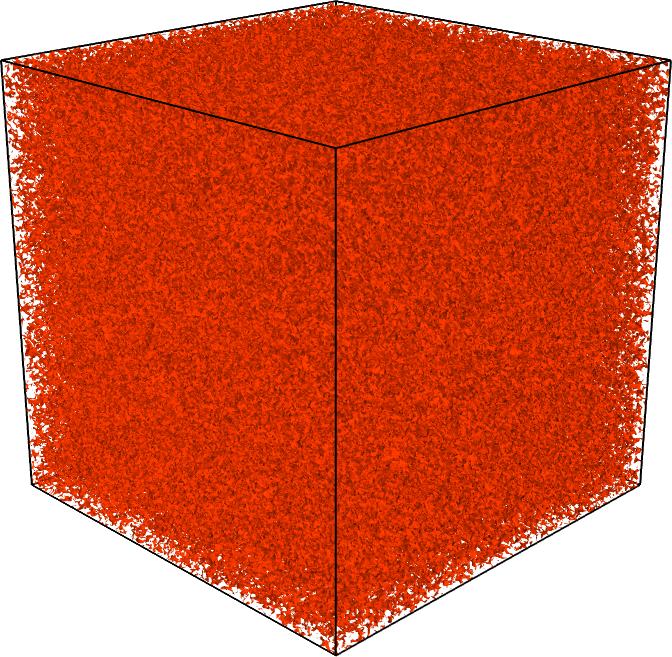
\includegraphics[width=0.35\linewidth]{numerics/figures/mess3d}%
    \begin{minipage}[b]{0.2\linewidth}
      \centering
      \raisebox{3cm}{$\longrightarrow$}
    \end{minipage}% 
    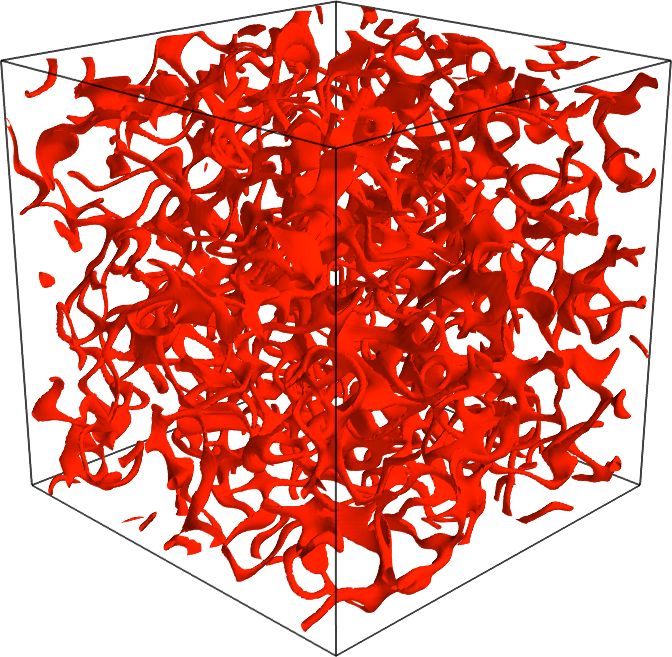
\includegraphics[width=0.35\linewidth]{numerics/figures/clean3d}
  \caption{(Left) Unfiltered wavefunction density, $|\psi|^2$, from a classical-field simulation with condensate fraction $\rho_0/\rho=0.22$ during equilibration. A vortex tangle is present but not visible by direct density visualisation. (Right) Filtered wavefunction density, $|\hat{\psi}|^2$, clearly showing the vortical structures in the gas.}\label{fig:quasicondensatefilter}
  \end{figure}

The choice of $k_c$ is facilitated by the the bimodal distribution of occupation numbers in the wavefunction, a distribution which develops naturally through propagation of the GPE. The high-$k$ part of the distribution is associated with the thermal excitations and low mode occupations. The low-$k$ part of the field is the quasi-condensate, characterised by macroscopic mode populations and superfluid ordering. $k_c$ is chosen as the boundary in $k$-space between the quasi-condensate and the thermal gas. Figure \ref{fig:quasicondensatefilter} demonstrates the filtering technique in action.

  	
\section{\label{section:linelength} Evaluation of vortex line-length in 3D}
For a given 3D wavefunction, $\Psi$, featuring a vortex distribution, the vortex volume $V_t$ (the total volume associated with the vortex cores) is evaluated by numerical integration of the inside of the vortex isosurface tubes obtained from the filtered density $|\hat \Psi|^2$, with an integration region of the whole numerical box.  Note that the isosurface level should be low enough to pick out vortex cores only (and not, e.g. fluctuations and waves), while large enough to contain sufficient grid points to allow a reasonable numerical evaluation of volume. In this work we use the isosurface level $0.04\langle |\hat{\Psi}|^2 \rangle$ (chosen so as to produce filtered vortex cores that are similar in radius to the true vortex core).  The volume calculation can be written $V_t = \int \Theta(0.04\langle |\hat{\Psi}|^2 \rangle - |\hat{\Psi}({\bf r})|^2)~{\rm d}V$, where $\Theta$ is the Heaviside step function. In practice the calculation of the vortex core volume can be efficiently performed by assigning a value of unity/zero to grid points located within/outside the isosurface tubes and directly integrating the result using the trapezium or Simpson's rule.

The total line length is then deduced by dividing $V_t$ by the cross-sectional area of a vortex core, $A_t$ (in effect, the average cross-sectional area of the isosurface tubes). The measured values of $V_t$ and $A_t$ will depend on the chosen isosurface level but, providing the vortex tubes are well-separated, their ratio (and hence the evaluated line length) will remain constant.  For closely-positioned vortex tubes, the isosurface level can affect whether the tubes appear as two separate tubes, or start to merge, and so will lead to deviations in this ratio.
\end{chapter}

  \part{Numerical Studies}
  \begin{chapter}{\label{cha:wake}Classical-like wakes behind elliptical obstacles in Bose-Einstein condensates}

\section{Introduction}
\begin{figure}[!ht]
\centering
  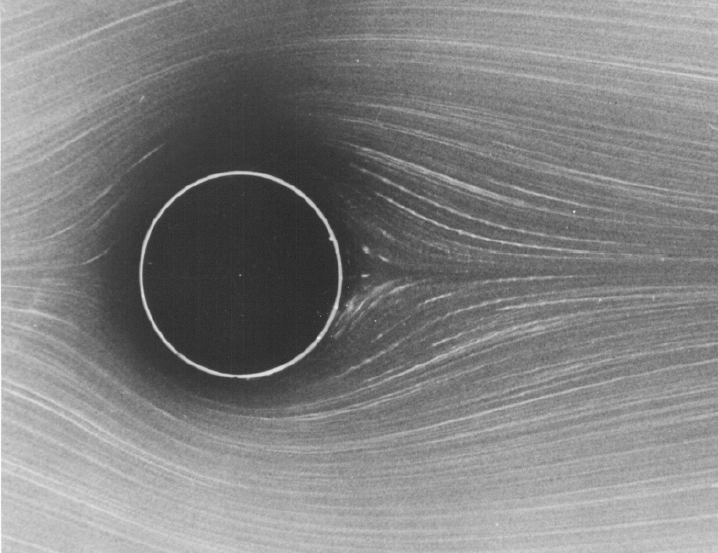
\includegraphics[height=2.08cm,angle=180]{wake/3.png}
  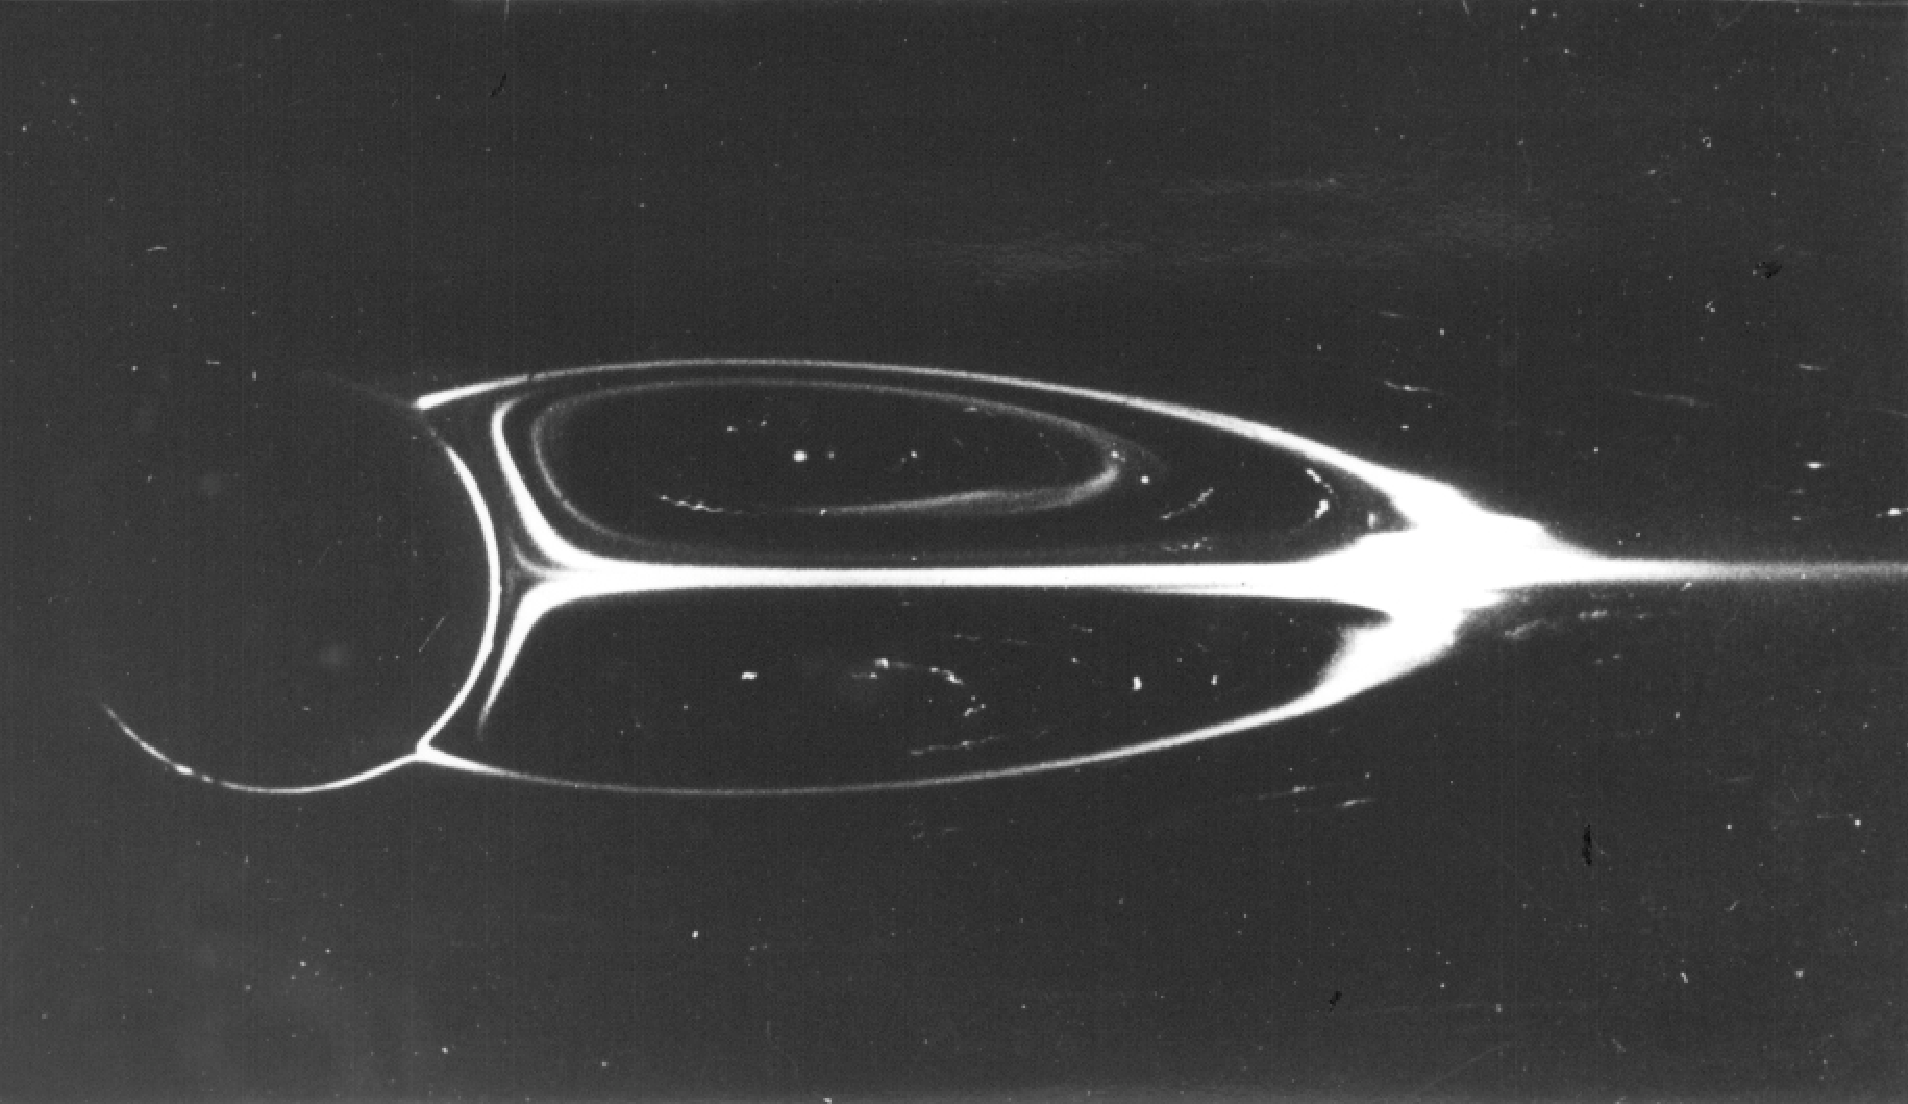
\includegraphics[width=0.24\textwidth,angle=180]{wake/taneda41}
  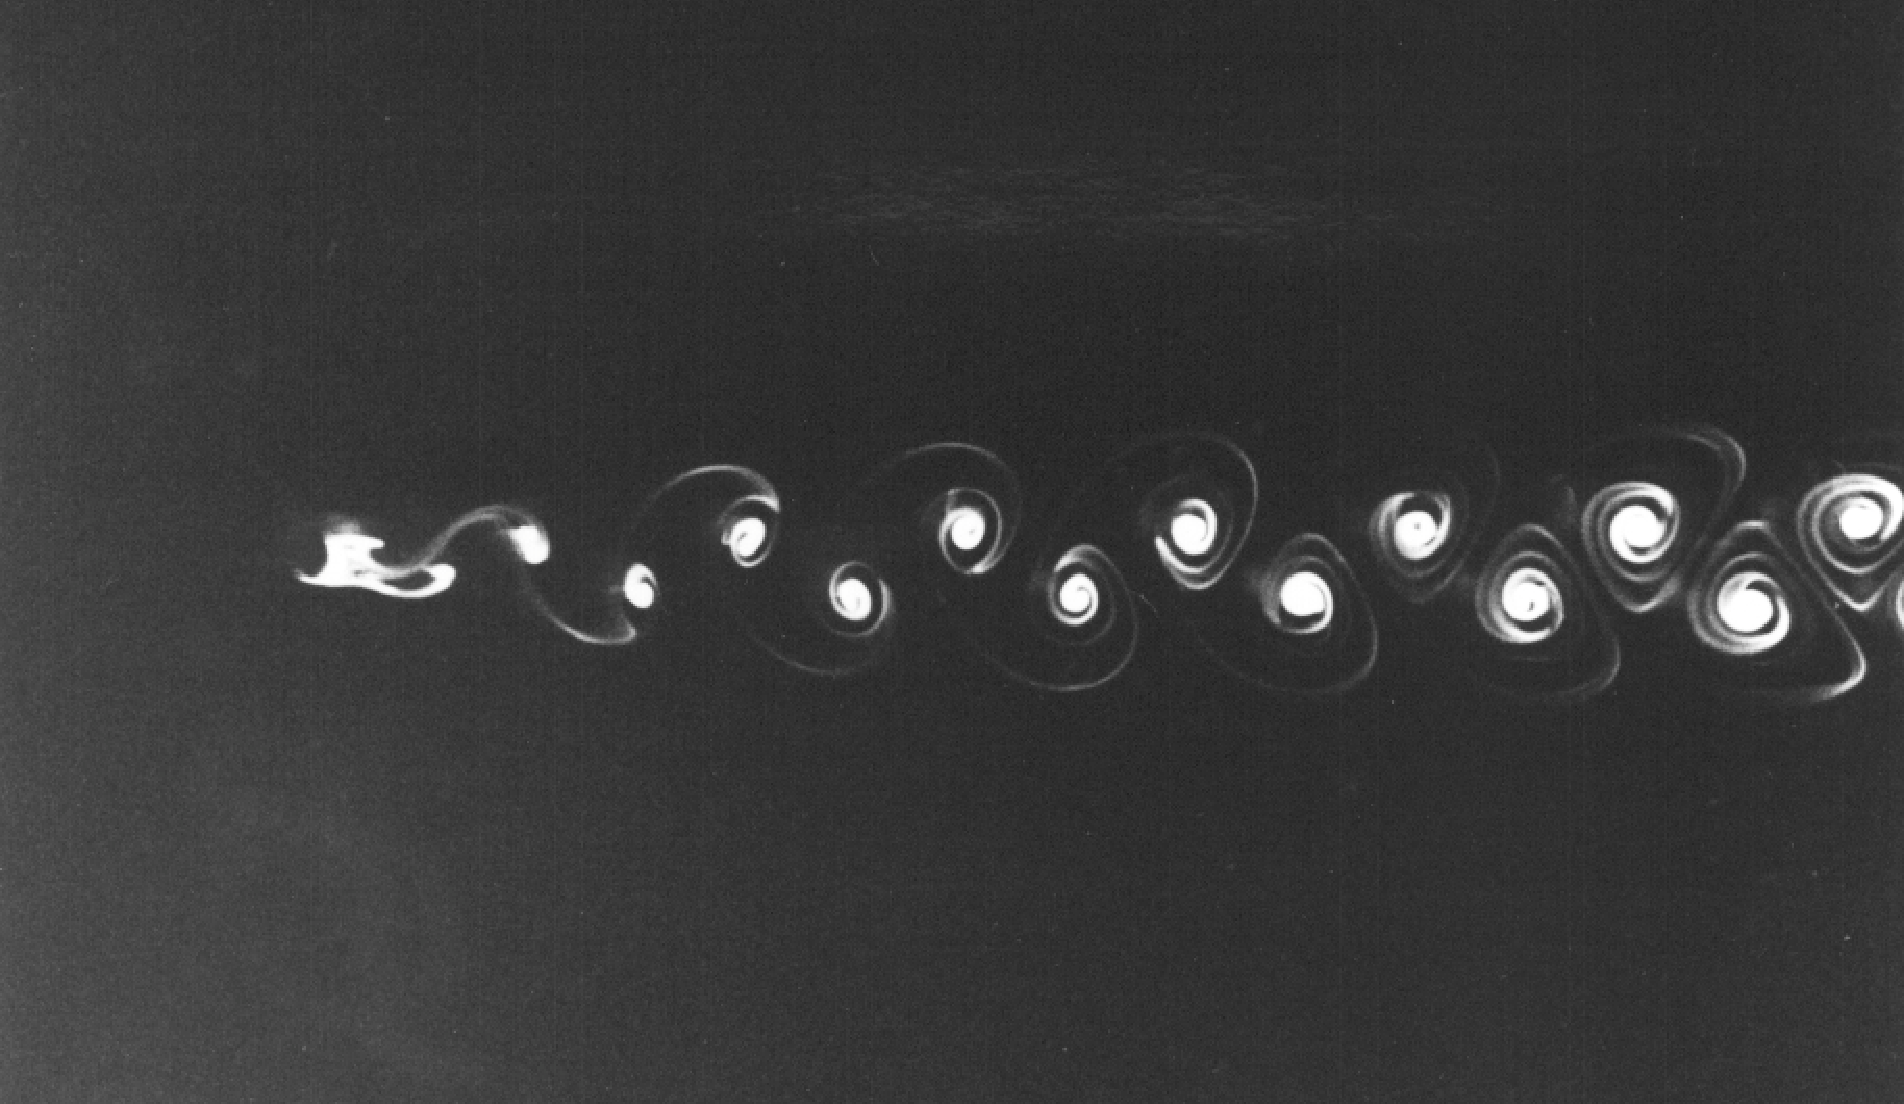
\includegraphics[width=0.24\textwidth,angle=180]{wake/taneda112}
    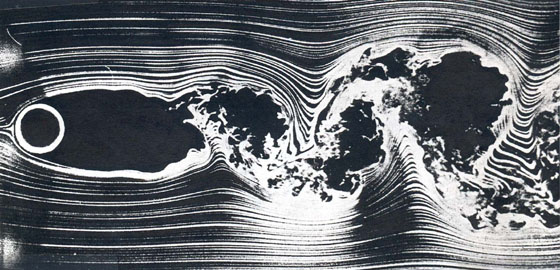
\includegraphics[width=0.29\textwidth,angle=180]{wake/turb.jpg}
  \caption{Classical viscous flow past a cylinder. From left to right: laminar flow ($\Rey=3.64$) \cite{taneda41}; steady symmetric wake behind the cylinder ($\Rey=41$) \cite{taneda41}; time-dependent B\'enard--von K\'arm\'an vortex street ($\Rey = 112$) \cite{taneda112}; and chaotic downstream wake ($\Rey > 10^5$) \cite{nagib}.} 
  \label{fig:taneda-imgs}
\end{figure}
Recent experimental \cite{Tabeling,Salort}, 
numerical \cite{Nore,Kobayashi,Laurie} 
and theoretical studies \cite{Lvov}
have highlighted similarities between turbulence in quantum
fluids and turbulence in ordinary (classical) fluids \cite{Frisch}.
In particular, it is found that, in
the idealized case of homogeneous isotropic conditions away from
boundaries, the distribution of kinetic energy over the 
length scales obeys the celebrated Kolmogorov scaling of 
classical turbulence \cite{barenghi}. This similarity is remarkable,
because a superfluid has zero viscosity and vorticity is not a continuous
field. In the more realistic presence of boundaries such as an obstacle or confining channel
walls, superfluid hydrodynamics is less understood, despite the large number of experiments in such scenarios. 

In a classical viscous fluid \cite{Frisch}, the prototype problem with
a boundary is the flow 
around a cylinder or a sphere (or, changing the frame of reference, 
the motion of a cylinder or a sphere in a fluid at rest).
The nature of such flow is determined by the Reynolds 
number $\Rey = vd/\nu$, where $v$ is the (assumed uniform)
flow's velocity away from the obstacle, $d$ is the obstacle's size,
and $\nu$ is the fluid's
kinematic viscosity. If $\Rey\lesssim50$, a steady symmetric 
wake forms behind the obstacle; if $10^2\lesssim\Rey\lesssim10^5$ the wake 
becomes asymmetric and time dependent, forming the famous 
B\'enard--von K\'arm\'an vortex street structure.  These cases are depicted in Figure \ref{fig:taneda-imgs}.  For even higher values of $\Rey$,
the flow becomes turbulent. 

What happens in a superfluid is not clear. Firstly, the superfluid has
zero viscosity ($\nu=0$) and hence $\Rey$ cannot be defined. Secondly,
experiments performed in superfluid helium confirm that the flow is affected
by the boundaries \cite{VanSciver1999,VanSciver2005}; unfortunately 
what is observed is not the flow pattern itself, but rather the
trajectories of tracer particles, whose
relation with the flow is still the subject
of investigations \cite{sergeev09}. Numerical simulations of three-dimensional (3D) superfluid flow around
an oscillating sphere performed using the vortex filament model
were not conclusive - quantum vortices did not appear to organise themselves
into a visible classical--like wake near the obstacle \cite{Hanninen,Fujiyama,goto08}.

Recent studies of the two-dimensional (2D) system have considered vortex emission and drag \cite{nore93,jma99,jma00,win00,huepe00}, the critical velocity \cite{zwerger00,crescimanno00,berloff2000,rica2001,pham2004}, the effect of inhomogeneous potentials \cite{win00,jackson98,fujimoto11}, the role of the obstacle parameters \cite{huepe00,jma00,aioi11}, and supersonic effects such as oblique dark solitons \cite{el06} and Cerenkov radiation \cite{carusotto06}. In this chapter we discuss the rich variety of quantum wake regimes, often in close analogue to the classical counterparts, which can be obtained via the simple modification of the obstacle to an {\it elliptical} shape. We explore these dynamics in a homogeneous system, which serves to demonstrate the salient behaviour of superfluid flow past an elliptical obstacle, away from boundaries and density inhomogeneities which influence the vortex dynamics.

\section{Model}

We consider an atomic Bose-Einstein condensate (BEC) moving relative to a laser-induced obstacle (imposed through 
an external potential), as realized experimentally in 3D \cite{Raman,Onofrio,Inouye,Neely} and quasi-2D condensates \cite{Neely}.  This scenario closely resembles that of the classical wake-problem \cite{taneda41,taneda112}.  On a much larger scale, a similar 
3D configuration has been experimentally realized in liquid helium 
\cite{VanSciver1999,VanSciver2005}.

The BEC, assumed to be weakly-interacting and at ultracold temperature, is modelled through the GPE as described in Section \ref{section:gpedimlesshomg}, transformed into the moving frame as in Section \ref{section:linearmovframe}. The external potential acting on the system $V({\bf r}, t)$ is taken to be zero everywhere, apart from a localized repulsive potential which represents the obstacle with the Gaussian shape described in Section \ref{section:3dcylinderpotential}. A key feature of this work is that the obstacle is modified so that it has ellipticity $\epsilon$, modifying the obstacle along the $x$ axis, parallel to the flow. Such a potential can be generated via the repulsive optical dipole force from an incident blue-detuned laser beam which is moved relative to the condensate either by deflection of the beam \cite{Raman,Onofrio,Inouye} or motion of the condensate itself when offset in a harmonic trap \cite{Neely,kwon_moon_14,kwon_2015a}.  While laser-induced obstacles generated to date have had a circular profile, elliptical modification of the Gaussian potential can be achieved via cylindrical focussing of the laser beam.   

The 2D (3D) system is simulated using the fourth-order Runge-Kutta method described in Section \ref{section:RK4} under periodic boundary conditions on a $2048 \times 512$ ($400 \times 150 \times 150$) grid with uniform spacing $\Delta_x=0.4\xi$. The computational box is sufficiently large that the boundary conditions do not play a role in vortex shedding.  The initial condition is the stationary state of the GPE (including obstacle potential) with $v=0$ as determined by the imaginary time convergence method described in Section \ref{section:imagTime}. Setting $V_0=100~\mu$ throughout, the external potential closely approximates an impenetrable obstacle. A small amount of noise is added to the initial condition to break symmetry: a random number between $-0.0005$ and $0.0005$ is added to both the real and imaginary parts of the initial wavefunction. To minimize initial generation of waves, $v$ is ramped up in time along a hyperbolic tangent curve, from $v=0$ at $t=0$ to its terminal value at $t\approx200~(\xi/c)$.

\section{Two-Dimensional Wakes}
\subsection{Vortex emission from circular obstacles}\label{subsec:circular}
The 2D scenario of an obstacle moving through a superfluid offers a simplified platform to consolidate analogues and disparities between classical and quantum fluids. In their pioneering simulations of the 2D nonlinear Schr\"odinger equation, Frisch {\it et al.} \cite{frisch92} observed the formation of vortex pairs in the flow past a circular obstacle. Although Frisch {\it et al.} considered a ``hard'' cylinder, it is also natural to employ a ``soft'' Gaussian potential (usually used in the context of atomic condensates). In practice this changes the quantitative, but not the qualitative, behaviour.  Sasaki {\it et al.} \cite{saito10} recently provided an extensive picture of 2D superflow past such a Gaussian obstacle.   The flow regimes are depicted in Fig. \ref{fig:denstypes}, based on simulations of the 2D GPE using similar parameters to \cite{saito10}.   At low flow velocity (a), the fluid undergoes smooth laminar flow around the obstacle.  The streamlines of this flow are symmetric about $x=0$, as in perfect potential flow.  At a critical flow velocity, the local fluid velocity (which is highest at the poles of the obstacle) exceeds the speed of sound, breaking Landau's criterion.  Vortex pairs of opposite sign are nucleated periodically and drift downstream, forming a collimated wake of vortex pairs which are widely separated from each other (b).  For higher velocities (c), alternating pairs of like-signed vortices are nucleated.  At even higher velocities, vortex nucleation becomes highly irregular (d), forming a chaotic downstream distribution of vortices and sound (density) waves.  These quantum fluid flow patterns bear some analogy to the classical flow patterns of Figure \ref{fig:taneda-imgs}, particularly for the laminar flow and chaotic regimes.  The alternating like-signed vortices form a somewhat primitive analogue of the B\'enard--von K\'arm\'an vortex street, while the vortex-antivortex pairs have no obvious classical analogue.  

\begin{figure}
(a) \hspace{7.2cm}(b)\\
\begin{tikzpicture}
  \begin{axis}[ylabel near ticks,xlabel near ticks,
      axis on top,
      width=0.5\linewidth,
      xlabel=$x/\xi$,
      ylabel=$y/\xi$,
      unit vector ratio=1 1 1,
      xmin = 190,
      xmax = 410,
      ymin = -45,
      ymax = 45,
      major tick length = 0.07cm,
    ]
    \addplot graphics [xmin=190,xmax=410,ymin=-45,ymax=45] {wake/quiver3};
  \end{axis}
\end{tikzpicture}
\begin{tikzpicture}
  \begin{axis}[ylabel near ticks,xlabel near ticks,
      axis on top,
      width=0.5\linewidth,
      xlabel=$x/\xi$,
      ylabel=$y/\xi$,
      unit vector ratio=1 1 1,
      xmin = 190,
      xmax = 410,
      ymin = -45,
      ymax = 45,
      major tick length = 0.07cm,
    ]
    \addplot graphics [xmin=190,xmax=410,ymin=-45,ymax=45] {wake/pairs_circle2};
  \end{axis}
\end{tikzpicture}\\
(c) \hspace{7.2cm}(d)\\
\begin{tikzpicture}
  \begin{axis}[ylabel near ticks,xlabel near ticks,
      axis on top,
      width=0.5\linewidth,
      xlabel=$x/\xi$,
      ylabel=$y/\xi$,
      unit vector ratio=1 1 1,
      xmin = 190,
      xmax = 410,
      ymin = -45,
      ymax = 45,
      major tick length = 0.07cm,
    ]
    \addplot graphics [xmin=190,xmax=410,ymin=-45,ymax=45] {wake/likesign_circle2};
  \end{axis}
\end{tikzpicture}
\begin{tikzpicture}
  \begin{axis}[ylabel near ticks,xlabel near ticks,
      axis on top,
      width=0.5\linewidth,
      xlabel=$x/\xi$,
      ylabel=$y/\xi$,
      unit vector ratio=1 1 1,
      xmin = 190,
      xmax = 410,
      ymin = -45,
      ymax = 45,
      major tick length = 0.07cm,
    ]
    \addplot graphics [xmin=190,xmax=410,ymin=-45,ymax=45] {wake/noise_circle2};
  \end{axis}
\end{tikzpicture}\\
  \caption{\label{fig:denstypes} Condensate density during flow past a circular obstacle ($d = 5\xi$) at various flow speeds. For reference the critical velocity here is $v_c \approx 0.36~c$.  (a) Laminar flow at a sub-critical flow speed ($v=0.3~c$).  The fluid velocity vector field and two streamlines illustrate the flow pattern. (b) Nucleation of vortex-antivortex pairs ($v=0.365~c$).  (c) Nucleation of like-signed vortex pairs ($v=0.37~c$). (d)  Chaotic vortex nucleation and generation of strong sound waves, forming a turbulent wake ($v=0.9~c$).}
\end{figure}

\subsection{Vortex emission from elliptical obstacles}
Consider, for illustration, an elliptical obstacle of size $d=5\xi$ and ellipticity $\epsilon=3$ moving at speed $v=0.365~c$.  This speed exceeds the critical velocity for the obstacle at that ellipticity, and so quantum vortices nucleate and trail behind the obstacle to form a wake [Figure \ref{fig:denstraj}(a)].  Sound waves generated by the obstacle have little effect on the vortex dynamics. At early times [Figure \ref{fig:denstraj}(a)(i)], the vortex shedding occurs through the symmetric generation of vortex-antivortex pairs, leading to a collimated and symmetric wake behind the obstacle.  This is in qualitative agreement with observations for circular obstacles \cite{frisch92,nore93,win00,huepe00} shown in Section \ref{subsec:circular}, although for the same obstacle velocity and size, the elliptical obstacle induces a higher frequency of vortex emission and thus a denser wake. 

At later times [Figure \ref{fig:denstraj}(a)(ii)], the flow becomes asymmetric due to the known instability of symmetric wakes \cite{nore93}.  A striking pattern emerges whereby distinct clusters of co-rotating vortices (of the order of 8 vortices in each cluster) develop downstream of the obstacle.  Each cluster contains vortices of the same sign and adjacent clusters have alternating sign.  These clusters form a B\'enard--von K\'arm\'an vortex street downstream from the obstacle, confirming the intuition that a sufficiently large number of quanta of circulation reproduce classical physics.  Here, the ellipticity of the obstacle facilitates the formation of this street; the relatively high rate of vortex emission leads to a greater interaction between vortices in the wake which in turn promotes clustering.  This is in contrast to Section \ref{subsec:circular} where vortex pairs (clusters of only 2) are produced; the vortex emission rate and hence their subsequent interaction is insufficient to induce large scale clustering.

\begin{figure}
(a) \hspace{2.5cm} (i)  $t = 1000 ~(\xi/c)$ \hspace{2.4cm} \hspace{1.8cm} (ii)   $t= 3500~ (\xi/c)$\\
\begin{tikzpicture}
  \begin{axis}[ylabel near ticks,xlabel near ticks,
      axis on top,
      width=0.5\linewidth,
      xlabel=$x/\xi$,
      ylabel=$y/\xi$,
      unit vector ratio=1 1 1,
      xmin = 150,
      xmax = 380,
      ymin = -45,
      ymax = 45,
      major tick length = 0.07cm,
    ]
    \addplot graphics [xmin=150,xmax=380,ymin=-45,ymax=45] {wake/figure2ai-dens2};
  \end{axis}
\end{tikzpicture}
\begin{tikzpicture}
  \begin{axis}[ylabel near ticks,xlabel near ticks,
      axis on top,
      width=0.5\linewidth,
      xlabel=$x/\xi$,
      ylabel=$y/\xi$,
      unit vector ratio=1 1 1,
      xmin = 150,
      xmax = 380,
      ymin = -45,
      ymax = 45,
      major tick length = 0.07cm,
    ]
    \addplot graphics [xmin=150,xmax=380,ymin=-45,ymax=45] {wake/figure2aii-dens2};
  \end{axis}
\end{tikzpicture}\\
(b)\hspace{2.5cm} (i)  $t = 0-1500 ~(\xi/c)$ \hspace{2.4cm} \hspace{1.2cm} (ii)   $t= 3500~ (\xi/c)$\\
\begin{tikzpicture}
  \begin{axis}[ylabel near ticks,xlabel near ticks,
      axis on top,
      width=0.5\linewidth,
      xlabel=$x/\xi$,
      ylabel=$y/\xi$,
      unit vector ratio=1 1 1,
      xmin = 150,
      xmax = 380,
      ymin = -45,
      ymax = 45,
      major tick length = 0.07cm,
    ]
    \addplot graphics [xmin=150,xmax=380,ymin=-45,ymax=45] {wake/figure2bi-raw};
  \end{axis}
\end{tikzpicture}
\begin{tikzpicture}
  \begin{axis}[ylabel near ticks,xlabel near ticks,
      axis on top,
      width=0.5\linewidth,
      xlabel=$x/\xi$,
      ylabel=$y/\xi$,
      unit vector ratio=1 1 1,
      xmin = 150,
      xmax = 380,
      ymin = -45,
      ymax = 45,
      major tick length = 0.07cm,
    ]
    \addplot graphics [xmin=150,xmax=380,ymin=-45,ymax=45] {wake/figure2bii-raw};
  \end{axis}
\end{tikzpicture}
  \caption{Snapshots showing the (a) density profile and (b) vortex trajectories during vortex shedding from an elliptical object ($\varepsilon = 3$) at (i) early times and (ii) later times.  The obstacle has speed $v=0.52c$ and size $d = 5\xi$. Red and blue lines represent vortices of oppositely quantized circulation. At early $t$, a symmetric wake similar to a classical fluid with low $Re$ forms. Symmetry breaks at $t\approx1500~(\xi/c)$ at which point vortex motion becomes disordered. In this case the initial condition is noise-free.}
  \label{fig:denstraj}
\end{figure}

The vortex trajectories shown in Figure \ref{fig:denstraj}(b) provide visualisation of the time-integrated nature of the wake.   At early times (i), we see that the vortex trajectories are symmetric, forming a flow pattern in striking analogue to the classical wake at low $Re$.  The generic development of vortex trajectories is as follows.  Pairs of singly-quantized vortices of opposite sign peel off from the poles of the obstacle and interact with each other as vortex-antivortex pairs.  Each pair propagates in the positive $x$ direction with approximate velocity $\hbar/(md_p)$ \cite{saito10}, where $d_p$ is the pair separation \cite{Donnelly};  the pair's velocity is less than the obstacle's velocity and so it drifts behind the obstacle.  As the pair moves further away from the obstacle, its separation decreases and its velocity increases, such that it begins to catch the obstacle up.  Once the pair is sufficiently close to the obstacle, it again separates and slows down, then the cycle repeats.  As more vortices are nucleated, two distinct clusters of like-circulation form.  Nucleated pairs then travel around the outside of the existing cluster before contracting, speeding up and travelling through the middle of the clusters towards the obstacle.  The clusters grow until they reach a maximum size depending on the obstacle's size and speed.  Hereafter, nucleated vortex pairs travel around the outside of the two clusters and continue travelling downstream,  becoming lost from the main wake. 
 
\subsection{Formation of the B\'enard--von K\'arm\'an vortex street}
\begin{figure}
(a) \hspace{7.2cm} (b)\\
\begin{tikzpicture}
  \begin{axis}[ylabel near ticks,xlabel near ticks,
      axis on top,
      width=0.485\linewidth,
      xlabel=$x/\xi$,
      ylabel=$y/\xi$,
      unit vector ratio=1 1 1,
      xmin=170,xmax=405,ymin=-55,ymax=55,
      major tick length = 0.07cm,
    ]
    \addplot graphics [xmin=170,xmax=405,ymin=-55,ymax=55] {wake/figure3a-raw};
  \end{axis}
\end{tikzpicture}
\begin{tikzpicture}
  \begin{axis}[ylabel near ticks,xlabel near ticks,
      axis on top,
      width=0.485\linewidth,
      xlabel=$x/\xi$,
      ylabel=$y/\xi$,
      unit vector ratio=1 1 1,
      xmin=170,xmax=405,ymin=-55,ymax=55,
      major tick length = 0.07cm,
    ]
    \addplot graphics [xmin=170,xmax=405,ymin=-55,ymax=55] {wake/figure3b-raw};
  \end{axis}
\end{tikzpicture}\\
(c)\hspace{7.2cm} (d)\\
\begin{tikzpicture}
  \begin{axis}[ylabel near ticks,xlabel near ticks,
      axis on top,
      width=0.485\linewidth,
      xlabel=$x/\xi$,
      ylabel=$y/\xi$,
      unit vector ratio=1 1 1,
      xmin=170,xmax=405,ymin=-55,ymax=55,
      major tick length = 0.07cm,
    ]
    \addplot graphics [xmin=170,xmax=405,ymin=-55,ymax=55] {wake/figure3c-raw};
  \end{axis}
\end{tikzpicture}
\begin{tikzpicture}
  \begin{axis}[ylabel near ticks,xlabel near ticks,
      axis on top,
      width=0.485\linewidth,
      xlabel=$x/\xi$,
      ylabel=$y/\xi$,
      unit vector ratio=1 1 1,
      xmin=170,xmax=405,ymin=-55,ymax=55,
      major tick length = 0.07cm,
    ]
    \addplot graphics [xmin=170,xmax=405,ymin=-55,ymax=55] {wake/figure3d-raw};
  \end{axis}
\end{tikzpicture}
  \caption{\label{fig:progress} Snapshots of vortex locations during the motion of an elliptical object ($d=5\xi$ and $\varepsilon=3$) at speed $v=0.52~c$ in the presence of small-amplitude noise at $t=0$.  The snapshots are at times (a) $t=450$, (b) $900$, (c) $1000$ and (d) $1100~(\xi/c)$.  Red/blue circles represent vortices with quanta of circulation $+1/-1$.  
The wake forms into clusters of like-circulation that continue to be produced, in analogy to the classical B\'enard--von K\'arm\'an vortex street from a cylinder.}
\end{figure}
Once the symmetry of the wake is broken, vortices no longer separate into two distinct clusters of like-circulation. Existing vortices and newly-nucleated vortices mix together behind the obstacle. %However it is apparent in Figure \ref{fig:denstraj}(b)(ii) that, on average, positive vortices drift to $y>0$ while negative vortices prefer to drift to $y<0$.
To accelerate the formation of the asymmetric wake, we subsequently seed the initial condition with noise.  Figure \ref{fig:progress} shows the vortex locations at various stages of the evolution. The initial symmetry of the wake [Figure \ref{fig:progress}(a)] breaks at $t \approx 450 (\xi/c)$, with the wake splitting into several clusters. The velocity field around the obstacle is affected: it depends on time and the distance of the nearest cluster of vortices. The obstacle no longer simultaneously produces vortex-antivortex pairs, but now generates a series of like-signed vortices.  Since like-signed vortices are known to co-rotate, these vortices group into clusters which slowly rotate.  This cluster effects the velocity field once more, causing a cluster of opposite signed vortices to be produced. This process then repeats such that clusters of like signed vortices are then produced behind the obstacle, much like vorticity in the classical vortex street behind a cylinder.  While some positive clusters contain negative vortices and vice versa, the overall pattern is still a time-dependent B\'enard--von K\'arm\'an vortex street.

For clusters consisting of pairs of vortices, it has been shown that they can survive downstream for a very long time \cite{saito10}.  However, for regimes with larger numbers of vortices in each cluster, the chaotic nature of vortex motion can cause originally tightly packed and circular clusters to easily stretch over large areas, form strange shapes, or even split into smaller clusters. Examples of this can be seen later in Figure \ref{fig:3x3grid}.


\subsection{Critical Velocity past an Elliptical Obstacle}
\label{sec:crit_vel}
\begin{figure}
\hspace{1.2cm}(a)\hspace{7cm} (b)
\begin{center}
\begin{tikzpicture}
  \begin{axis}[samples=72,ylabel near ticks,xlabel near ticks,
      width=0.45\linewidth,
        xlabel=$\varepsilon\phantom{d}$,
        ylabel=$v_c/c$,
        xmin=0.9,
        xmax=3.1,
        ymin=0.1,
        ymax=0.61,
        major tick length = 0.07cm]
    \addplot+[only marks, samples=30, error bars/y dir=both, error bars/y fixed=0.012,error bars/error bar style={thick},mark options={blue,scale=0.8}] file {wake/data/v_c_vs_epsilon.dat};
    \addplot+[mark=none,color=red,thick,dashed] {1/(1+x)};
    \addplot+[mark=none,color=black,thick] {((3/2)*(1+x)^2-(1/2))^(-1/2)};
  \end{axis}
  \end{tikzpicture}%
  \begin{tikzpicture}
  \begin{axis}[ylabel near ticks,xlabel near ticks,
        width=0.45\linewidth,
        xtick pos=left,
    ytick pos=left,
        xlabel=$d\phantom{\varepsilon}$,
        ylabel=$v_c/c$,
        xmin=0,
        xmax=11,
        ymin=0.1,
        ymax=0.61,
        major tick length = 0.07cm
      ]
      \addplot+[only marks,mark options={red,scale=0.8}, error bars/y dir=both, error bars/y fixed=0.012,error bars/error bar style={thick,red}] file {wake/data/v_c_vs_d_e1.dat};
      \addplot+[only marks,mark=triangle*,mark options={green}, error bars/y dir=both, error bars/y fixed=0.012,error bars/error bar style={thick,green}] file {wake/data/v_c_vs_d_e2.dat};
      \addplot+[only marks,mark=square*,mark options={blue,scale=0.75}, error bars/y dir=both, error bars/y fixed=0.012,error bars/error bar style={thick,blue}] file {wake/data/v_c_vs_d_e3.dat};
    \end{axis}
\end{tikzpicture}%
\end{center}
\caption{\label{fig:velplots}(a) Critical velocity against obstacle ellipticity $\varepsilon$, for $d=10\xi$.  Shown are the results the numerical simulations (blue bars), Equation (\ref{eq:crit1}) (dashed red line) and Equation (\ref{eq:crit2}) (solid black line). (b) Critical velocity (obtained numerically) versus the obstacle width $d$, for ellipticity $\varepsilon=1$ (red circles), $\varepsilon=2$ (green triangles) and $\varepsilon=3$ (blue squares).
}
\end{figure} 
We now investigate in what ways the ellipticity of the obstacle affects the critical velocity for vortex nucleation and nucleation frequency.  Figure \ref{fig:velplots}(a) shows the critical velocity for flow past the obstacle as a function of its ellipticity, taking the obstacle to have fixed width in the $y$-direction of $d=10\xi$.  We determine the critical velocity numerically by performing simulations with flow velocities increasing in steps of $\Delta_v=0.01\,c$ until vortices nucleate.  
For a circular object, we find that the critical velocity is $v_{\rm c}=0.355\pm 0.005~c$, consistent with predictions in the Eulerian ($d \gg \xi$) limit \cite{berloff2000,rica2001,pham2004}.  As the ellipticity is increased (i.e. the obstacle becomes narrower in $x$), the critical velocity decreases.  The modification of the critical velocity is significant: if $\varepsilon=3$, $v_{\rm c}$ is more than $40\%$ smaller than that for a circular obstacle. 

The rough dependence of $v_{\rm c}$ on $\varepsilon$ can be derived as follows.   According to Landau's criterion \cite{NozieresPines},  superfluidity breaks down when the fluid velocity exceeds the critical velocity $v_{\rm Lan}=\min \left[E(p)/p\right]$, where $p$ is the momentum of elementary excitations and $E(p)$ their energy.   The weakly-interacting Bose gas has the dispersion relation $E(p)=[ngp^2/m + p^4/(4m^2)]^{1/2}$, hence $v_{\rm Lan}=c$.

If an obstacle moves through the fluid with speed $v$, the local fluid velocity is enhanced near the obstacle so that the maximum local velocity, $v_{\rm max}$, exceeds $v$. By approximating the BEC as an inviscid Euler fluid, we can calculate the local velocity around the obstacle using the complex variable framework of potential flow. The maximum local velocity is then found to be at the poles with $v_{\rm max}=(1+\varepsilon)v$ \cite{Schlichting42}, and the estimated Landau critical velocity becomes,
\begin{equation}
\frac{v_{c1}}{c} = \frac{1}{1+\varepsilon}.
\label{eq:crit1}
\end{equation}
This estimate is shown as dashed red line in Figure \ref{fig:velplots}(a), capturing the general shape of the relationship, but not the exact values for $v_{\rm c}$.
%While this result assumes constant density, a first order correction can be made by using Bernoulli's theorem to model the reduction in local density near the obstacle (due to the enhanced local fluid velocity) which in turn reduces the local speed of sound $c(x,y)=\sqrt{n(x,y)g/m}$ \cite{win01}.  This then leads to the modified result,

Equation \ref{eq:crit1} is derived for incompressible potential flow, however, the GPE describes a compressible fluid and so the local density, $n(\bf r) = |\psi|^2$, in regions of high velocity is reduced. Ignoring the quantum pressure, the density (and therefore speed of sound) is reduced according to Bernoilli's equation \cite{win01},
\begin{equation}
1+\frac{v^2}{2} = n(u)+\frac{u^2}{2},
\label{eq:bern}
\end{equation}
where $u(\bf r)$ is the local velocity. We substitute the maximum local velocity, $v_{\rm max}=(1+\varepsilon)v$, into Equation \ref{eq:bern} to find the local density at that point,
\begin{equation*}
n(v_{\rm max}) = 1+\frac{1}{2}[1-(1+\epsilon)^2]v^2.
\end{equation*}
The local speed of sound is $c_{\rm local}=\sqrt{n}$ and so at the point of maximal velocity,
\begin{equation*}
c_{\rm local} = \sqrt{1+\frac{1}{2}[1-(1+\epsilon)^2]v^2}.
\end{equation*}
We use the resulting local speed of sound and the Landau criterion to find a corrected estimate of the critical velocity for the break down of superfluidity, 
\begin{equation}
\frac{v_{c2}}{c} = \left [\frac{3}{2}(1+\varepsilon)^2 - \frac{1}{2}\right]^{-\frac{1}{2}}.
\label{eq:crit2}
\end{equation}
This relation (solid blue line in Figure \ref{fig:velplots}) gives good agreement with the computed values of $v_{\rm c}$.  The deviation for $\varepsilon \sim 1$ has been noted elsewhere \cite{rica2001}, and can be remedied using higher order corrections taking into account the quantum pressure term.

From studies on circular objects, it is known that $v_{\rm c}$ depends on the obstacle's shape at small diameters, where boundary layer effects are significant; $v_{\rm c}$ approaches the ``Eulerian" value only for large diameters $d \gg \xi$ \cite{huepe00,rica2001}.  The variation of $v_{\rm c}$ with the obstacle width $d$ is shown in Figure \ref{fig:velplots} (inset).  For $d=10\xi$, the critical velocity effectively reaches its asymptotic value, while at smaller widths, it is much larger.   

\subsection{Role of Obstacle Size and Ellipticity on the Wake}
\label{sec:ellipt}
\begin{figure}
\begin{center}
\begin{minipage}{0.33\linewidth}%
\vspace{-0.3cm}(a)~(i)\\\vspace{-0.3cm}%
\begin{tikzpicture}%
\begin{axis}[axis on top,width=\linewidth,xlabel={},ylabel=$y/\xi$,yticklabels={,,-20,0,20},xticklabels={,,},unit vector ratio=1 1 1,xmin=170,xmax=405,ymin=-40,ymax=40,major tick length = 0.07cm] 
\addplot graphics [xmin=170,xmax=405,ymin=-40,ymax=40] {wake/figure5zi-raw};
\end{axis}%
\end{tikzpicture}\\%
\vspace{-0.3cm}(b)\\\vspace{-0.3cm}%
\begin{tikzpicture}%
\begin{axis}[axis on top,width=\linewidth,xlabel={},ylabel=$y/\xi$,yticklabels={,,-20,0,20},xticklabels={,,},unit vector ratio=1 1 1,xmin=170,xmax=405,ymin=-40,ymax=40,major tick length = 0.07cm]
\addplot graphics [xmin=170,xmax=405,ymin=-40,ymax=40] {wake/figure5zzi-raw};
\end{axis}%
\end{tikzpicture}\\%
\vspace{-0.3cm}(c)\\\vspace{-0.3cm}%
\begin{tikzpicture}%
\begin{axis}[axis on top,width=\linewidth,xlabel={},ylabel=$y/\xi$,yticklabels={,,-20,0,20},xticklabels={,,},unit vector ratio=1 1 1,xmin=170,xmax=405,ymin=-40,ymax=40,major tick length = 0.07cm]
\addplot graphics [xmin=170,xmax=405,ymin=-40,ymax=40] {wake/figure5ai-raw};
\end{axis}%
\end{tikzpicture}\\%
\vspace{-0.3cm}(d)\\\vspace{-0.3cm}%
\begin{tikzpicture}%
\begin{axis}[axis on top,width=\linewidth,xlabel={},ylabel=$y/\xi$,yticklabels={,,-20,0,20},xticklabels={,,},unit vector ratio=1 1 1,xmin=170,xmax=405,ymin=-40,ymax=40,major tick length = 0.07cm]
\addplot graphics [xmin=170,xmax=405,ymin=-40,ymax=40] {wake/figure5bi-raw};
\end{axis}%
\end{tikzpicture}\\%
\vspace{-0.3cm}(e)\\\vspace{-0.3cm}%
\begin{tikzpicture}%
\begin{axis}[axis on top,width=\linewidth,xlabel=$x/\xi$,ylabel=$y/\xi$,yticklabels={,,-20,0,20},unit vector ratio=1 1 1,xmin=170,xmax=405,ymin=-40,ymax=40,major tick length = 0.07cm]
\addplot graphics [xmin=170,xmax=405,ymin=-40,ymax=40] {wake/figure5ci-raw};
\end{axis}%
\end{tikzpicture}%
\end{minipage}%
\begin{minipage}{0.33\linewidth}%
\vspace{-0.3cm}(ii)\\\vspace{-0.3cm}%
\begin{tikzpicture}%
\begin{axis}[axis on top,width=\linewidth,xlabel={},ylabel={},yticklabels={,,},xticklabels={,,},unit vector ratio=1 1 1,xmin=170,xmax=405,ymin=-40,ymax=40,major tick length = 0.07cm] 
\addplot graphics [xmin=170,xmax=405,ymin=-40,ymax=40] {wake/figure5zii-raw};
\end{axis}%
\end{tikzpicture}\\%
\vspace{-0.3cm}\phantom{(a)}\\\vspace{-0.3cm}%
\begin{tikzpicture}%
\begin{axis}[axis on top,width=\linewidth,xlabel={},ylabel={},yticklabels={,,},xticklabels={,,},unit vector ratio=1 1 1,xmin=170,xmax=405,ymin=-40,ymax=40,major tick length = 0.07cm]
\addplot graphics [xmin=170,xmax=405,ymin=-40,ymax=40] {wake/figure5zzii-raw};
\end{axis}%
\end{tikzpicture}\\%
\vspace{-0.3cm}\phantom{(a)}\\\vspace{-0.3cm}%
\begin{tikzpicture}%
\begin{axis}[axis on top,width=\linewidth,xlabel={},ylabel={},yticklabels={,,},xticklabels={,,},unit vector ratio=1 1 1,xmin=170,xmax=405,ymin=-40,ymax=40,major tick length = 0.07cm]
\addplot graphics [xmin=170,xmax=405,ymin=-40,ymax=40] {wake/figure5aii-raw};
\end{axis}%
\end{tikzpicture}\\%
\vspace{-0.3cm}\phantom{(a)}\\\vspace{-0.3cm}%
\begin{tikzpicture}%
\begin{axis}[axis on top,width=\linewidth,xlabel={},ylabel={},yticklabels={,,},xticklabels={,,},unit vector ratio=1 1 1,xmin=170,xmax=405,ymin=-40,ymax=40,major tick length = 0.07cm]
\addplot graphics [xmin=170,xmax=405,ymin=-40,ymax=40] {wake/figure5bii-raw};
\end{axis}%
\end{tikzpicture}\\%
\vspace{-0.3cm}\phantom{(a)}\\\vspace{-0.3cm}%
\begin{tikzpicture}%
\begin{axis}[axis on top,width=\linewidth,xlabel={$x/\xi$},ylabel={},yticklabels={,,},unit vector ratio=1 1 1,xmin=170,xmax=405,ymin=-40,ymax=40,major tick length = 0.07cm]
\addplot graphics [xmin=170,xmax=405,ymin=-40,ymax=40] {wake/figure5cii-raw};
\end{axis}%
\end{tikzpicture}%
\end{minipage}\hspace{-0.06\linewidth}%
\begin{minipage}{0.33\linewidth}%
\vspace{-0.3cm}(iii)\\\vspace{-0.3cm}%
\begin{tikzpicture}%
\begin{axis}[axis on top,width=\linewidth,xlabel={},ylabel={},yticklabels={,,},xticklabels={,,},unit vector ratio=1 1 1,xmin=170,xmax=405,ymin=-40,ymax=40,major tick length = 0.07cm] 
\addplot graphics [xmin=170,xmax=405,ymin=-40,ymax=40] {wake/figure5ziii-raw};
\end{axis}%
\end{tikzpicture}\\%
\vspace{-0.3cm}\phantom{(a)}\\\vspace{-0.3cm}%
\begin{tikzpicture}%
\begin{axis}[axis on top,width=\linewidth,xlabel={},ylabel={},yticklabels={,,},xticklabels={,,},unit vector ratio=1 1 1,xmin=170,xmax=405,ymin=-40,ymax=40,major tick length = 0.07cm]
\addplot graphics [xmin=170,xmax=405,ymin=-40,ymax=40] {wake/figure5zziii-raw};
\end{axis}%
\end{tikzpicture}\\%
\vspace{-0.3cm}\phantom{(a)}\\\vspace{-0.3cm}%
\begin{tikzpicture}%
\begin{axis}[axis on top,width=\linewidth,xlabel={},ylabel={},yticklabels={,,},xticklabels={,,},unit vector ratio=1 1 1,xmin=170,xmax=405,ymin=-40,ymax=40,major tick length = 0.07cm]
\addplot graphics [xmin=170,xmax=405,ymin=-40,ymax=40] {wake/figure5aiii-raw};
\end{axis}%
\end{tikzpicture}\\%
\vspace{-0.3cm}\phantom{(a)}\\\vspace{-0.3cm}%
\begin{tikzpicture}%
\begin{axis}[axis on top,width=\linewidth,xlabel={},ylabel={},yticklabels={,,},xticklabels={,,},unit vector ratio=1 1 1,xmin=170,xmax=405,ymin=-40,ymax=40,major tick length = 0.07cm]
\addplot graphics [xmin=170,xmax=405,ymin=-40,ymax=40] {wake/figure5biii-raw};
\end{axis}%
\end{tikzpicture}\\%
\vspace{-0.3cm}\phantom{(a)}\\\vspace{-0.3cm}%
\begin{tikzpicture}%
\begin{axis}[axis on top,width=\linewidth,xlabel={$x/\xi$},ylabel={},yticklabels={,,},unit vector ratio=1 1 1,xmin=170,xmax=405,ymin=-40,ymax=40,major tick length = 0.07cm]
\addplot graphics [xmin=170,xmax=405,ymin=-40,ymax=40] {wake/figure5ciii-raw};
\end{axis}
\end{tikzpicture}%
\end{minipage}%
\end{center}
\caption{\label{fig:3x3grid}Snapshots of the vortex positions for various obstacle parameters, at $t=2000~(\xi/c)$. Shown are obstacles corresponding to (a) $\varepsilon=0.5$ and $d=5\xi$, (a) $\varepsilon=0.75$ and $d=5\xi$, (c) $\varepsilon=1$ and $d=5\xi$, (d) $\varepsilon=2$ and $d=5\xi$, and (e) $\varepsilon=2$ and $d=10\xi$, at the velocities (i) $v=0.32c$, (ii) $v=0.40c$, and (iii) $v=0.48c$.  Red/blue circles represent vortices with quanta of circulation $+1/-1$.}
\end{figure}
During the initial symmetric phase of vortex nucleation, the wakes generated by the obstacle have the same qualitative structure shown in Figure \ref{fig:denstraj}(b) (i).  However, once the wake becomes asymmetric, the nature of the clusters that form are highly dependent on the velocity and shape of the obstacle. Figure \ref{fig:3x3grid} shows wakes generated for various obstacle parameters, all captured at the same time $t=2000~(\xi/c)$. As predicted in the previous section, for an increased $\varepsilon$, the critical velocity for vortex nucleation is reduced. Conversely, reducing $\varepsilon<1$ causes the critical velocity to increase to the point of no vortices being produced for any of the tested velocities. By visual inspection of the clusters that form in Figure \ref{fig:3x3grid}, it can be seen that that any increase of size, ellipticity or velocity of the obstacle increases the number of vortices in the wake's clusters. We further explore this clustering behaviour and explain its roots in Section \ref{sec:clusteringwake}.

\subsection{Vortex Clustering}\label{sec:clusteringwake}
We have shown that the B\'enard--von K\'arm\'an vortex street forms through the clustering of like-signed vortices. Methods of quantifying the clustering of vortices in quantum fluids have been explored in the literature \cite{white12,reeves_billam_13,bagg12} and are described in detail in Section \ref{section:vortexclustering}.

We begin by quantifying the effect of ellipticity on vortex clustering using the $K$ and $L$ functions defined in Section \ref{section:ripleysk}. To interpret the results, the curve 
\begin{equation}
  L_\varepsilon(s) = \langle \hat{L}(\varepsilon,s) - s \rangle,
\end{equation}
is calculated. Here $s$ characterises the radius of the clustering and $\hat{L}(\varepsilon,s)$ is the estimate of the $L$ curve given by Equation \ref{eq:ripleysl}, measured at the time $t=2500~(\xi/c)$ for the three ellipticities $\varepsilon=1, 2, 3$. The average is performed for each value of $\varepsilon$, over 5 simulations with external flow velocities $v = 0.4,0.425,0.450,0.475,0.5~c$. When $L_\varepsilon(s)>0$, it is interpreted as evidence of clustering on the scale of $s$ for ellipticity $\varepsilon$. Conversely when $L_\varepsilon(s)<0$, it is interpreted as evidence of a sparsity of vortices (as compared to randomly placed points in space) on the scale of $s$ for ellipticity $\varepsilon$. The resulting curves are shown in Figure \ref{fig:ripleyLwake}.

\begin{figure}
\begin{center}
  \begin{tikzpicture}
    \begin{axis}[ylabel near ticks,xlabel near ticks,
          width=0.5\linewidth,
          samples=72,
          xtick pos=left,
          ytick pos=left,
          xlabel=$s/\xi$,
          ylabel=$L_\varepsilon$,
          xmin=0,
          xmax=200,
          major tick length = 0.07cm
        ]
        \addplot[ultra thin,gray] coordinates {(-600,0) (600,0)};
        \addplot+[thick,red,dashed,mark=none] file  {wake/data/L_vs_r_e1.dat};
        \addplot+[thick,green,dashdotted,mark=none] file  {wake/data/L_vs_r_e2.dat};
        \addplot+[thick,blue,mark=none] file  {wake/data/L_vs_r_e3.dat};
      \end{axis}
  \end{tikzpicture}
\end{center}
\caption{\label{fig:ripleyLwake} The clustering measurement $L_\varepsilon(s)$ for the three ellipticities $\varepsilon=1$ (red dashed line), $\varepsilon=2$ (green dot-dashed line), and $\varepsilon=3$ (blue solid line) (with obstacle size $d=5\xi$) averaged over 5 simulations for each $\varepsilon$ with external flow velocities $v = 0.4,0.425,0.450,0.475,0.5~c$.}
\end{figure}

All three curves show pronounced evidence of clustering at scales of $5\xi\lesssim s\lesssim 150\xi$. Lack of clustering is evident at $s\lesssim 5\xi$, this is to be expected: multiply charged vortices are unstable, preferring to decay into several vortices distinct in space, and so clustering is not expected on scales smaller than the radius of a vortex core (approximately $5\xi$). The lack of clustering at scales of $s \gtrsim 150\xi$ can be explained by the lack of vortices far from the obstacle in the $\pm y$ directions. As $\varepsilon$ increases, the peak value of $L_\varepsilon(s)$ also increases, showing evidence that an increase of ellipticity causes an increase of the spacial clustering of vortices in the fluid.

The $K$ and $L$ curves quantify the average spatial statistics of vortex clustering, but do not tell us the number of vortices present in clusters. We now utilize the more sophisticated Recursive Cluster Algorithm (RCA) of Reeves \emph{et. al.} \cite{reeves_billam_13} (described in Section \ref{section:reevesalgorithm}) to identify the number of vortices contained in clusters for different ellipticities and velocities. The use of RCA allows us to investigate how both velocity and ellipticity each affect vortex clustering. We record the number of clusters $N_c$ and the number of vortices in each cluster $N_i$, where $i$ is the cluster index. Then we determine the average number of vortices in the clusters, $\langle N \rangle = (1/N_c) \sum_{i=1}^{i=N_c} N_i$ as a function of obstacle velocity $v$ for three ellipticities $\varepsilon=1, 2$ and $3$, at times $t=500,510,\ldots,2500~(\xi/c)$. The results, plotted in Figure \ref{fig:Svslocal2}, show that increasing $v$ (above the critical velocity) causes $\langle N \rangle$ to increase and that, at fixed $v$, $\langle N \rangle$ increases with $\varepsilon$. 

\begin{figure}
\centering
\begin{tikzpicture}
\begin{axis}[samples = 72, ylabel near ticks,xlabel near ticks,
      width=0.5\linewidth,
      xtick pos=left,
      ytick pos=left,
      xlabel=$v/c$,
      ylabel=$\langle N \rangle$,
      xmin=0.28,
      xmax=0.52,
      ymin=0.2,
      ymax=9,
      major tick length = 0.07cm
    ]
    \addplot+[only marks,mark options={red},error bars/error bar style={red},  error bars/.cd,y dir=both,y explicit
    ] table[x=X,y=Y,y error=Y_error] {wake/data/n_vs_v_e1.dat};
    \addplot+[only marks,mark=triangle*,mark options={green},error bars/error bar style={green},  error bars/.cd,y dir=both,y explicit
    ] table[x=X,y=Y,y error=Y_error] {wake/data/n_vs_v_e2.dat};
    \addplot+[only marks,mark=square*,mark options={blue,scale=0.75},error bars/error bar style={blue},  error bars/.cd,y dir=both,y explicit
    ] table[x=X,y=Y,y error=Y_error] {wake/data/n_vs_v_e3.dat};
    \addplot+[mark=none,color=red,dashed] {28.1680*x-9.6560};
    \addplot+[mark=none,color=green,dashed] {29.2809*x-7.5794};
    \addplot+[mark=none,color=blue,dashed] {29.8248*x-6.4902};
  \end{axis}
\end{tikzpicture}
\caption{\label{fig:Svslocal2} Average number of vortices in the clusters as a function of the obstacle velocity $v$.  Shown are cases with $\varepsilon=1$ (red squares),  $\varepsilon=2$ (green circles) and $\varepsilon=3$ (blue triangles) with $d=5\xi$. Also shown is are linear fits to the data for each value of $\varepsilon$.}
\end{figure}

The behaviour of the quantities explored in this section, and therefore the reason that elliptical obstacles are efficient at producing classical-like wakes, can be explained by considering the shedding frequency of vortices. It is known that the shedding frequency increases with the velocity of the flow \cite{jma99} and for an elliptical obstacle, the combination of a reduced critical velocity and increased local velocity around the obstacle has the effect of increasing the shedding frequency with $\varepsilon$ and $d$. The overall result is that, when increasing any of $v$, $\varepsilon$ or $d$, more vortices are nucleated in a given time period, causing the cluster size to increase (explaining the behaviour of $L_\varepsilon$, $\langle N\rangle$, and the vortex clustering exhibited in Figure \ref{fig:3x3grid}). By further simulation at large obstacle velocity ($v\gtrsim0.6$), we also find that for all values of $\varepsilon$, the large velocity causes vortices to nucleate non-periodically, inducing an irregular flow without a visible B\'enard--von K\'arm\'an vortex street configuration, in agreement with previous simulations with circular obstacles of smaller diameter \cite{saito10}.

\section{Three-Dimensional Wakes}
We now generalize our results to 3D by considering quantum wakes in three-dimensional flow past a localized obstacle, as simulated via the 3D GPE with the 3D obstacle potential of Equation (\ref{eq:potential3D}).  Our results will confirm that the features observed in 2D wakes also arise in the 3D setting.  A comprehensive study of the parameter space is, however, not tractable in 3D due to the computational intensity of large scale 3D simulations.



\begin{figure}[!ht]
(a)\\
\begin{minipage}{0.5\linewidth}%
\centering
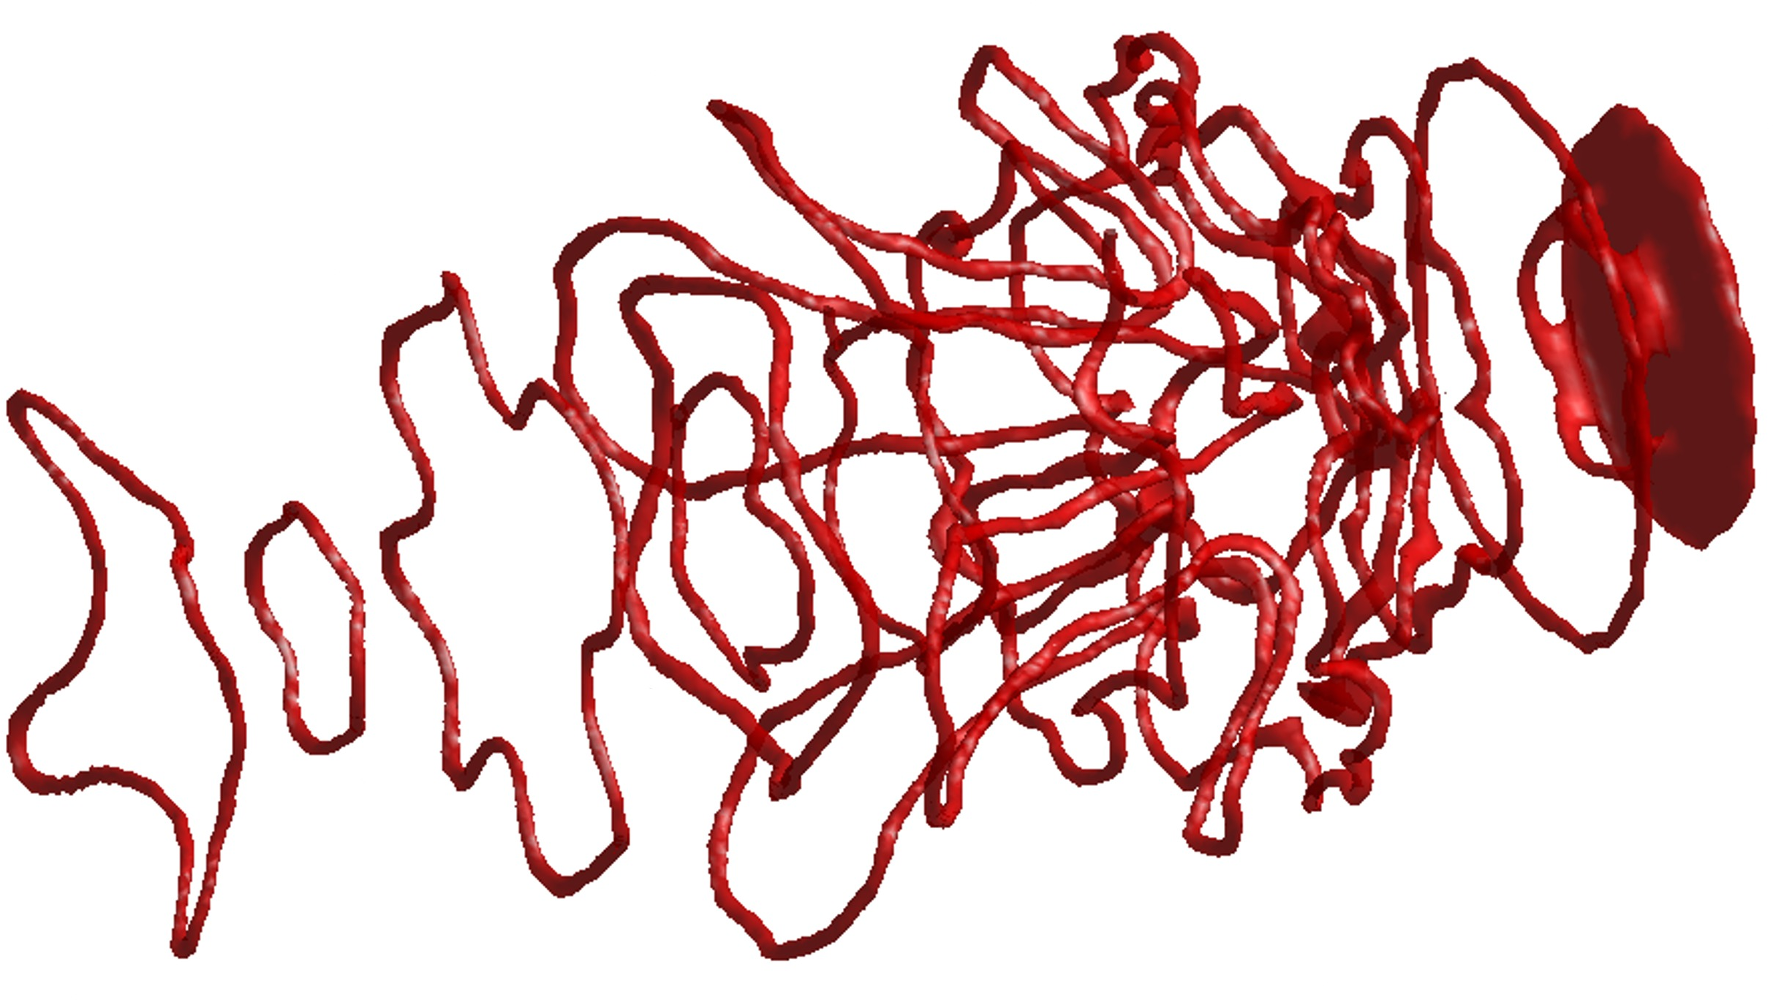
\includegraphics[width=0.9\linewidth]{wake/symwake}
\end{minipage}%
\begin{minipage}{0.5\linewidth}%
\vspace{-0.84\baselineskip}(b)\\
\begin{tikzpicture}[domain=-60:100]
  \begin{axis}[xlabel={$x$}, ylabel={$y$},
      xmin=-60,xmax=100,ymin=-35,ymax=35,
      major tick length = 0.07cm,
      width=\linewidth,
      unit vector ratio=1 1 1,
      scatter/classes={ 0={mark=*,blue},1={mark=o,red}},
      xlabel=$x/\xi$,
      ylabel=$y/\xi$,
      mark size = 0.7
      ]
  \draw[fill] (axis cs:86,0) ellipse [x radius= 1.7, y radius=11];
  \addplot[scatter, only marks,mark options={scale=2}, scatter src=\thisrow{class},
        error bars/.cd, y dir=both, x dir=both, y explicit, x explicit]
        table[x=x,y=y] {wake/symwakevort.dat};
  \end{axis}
\end{tikzpicture}\\%
(c)\\%
\begin{tikzpicture}
  \begin{axis}[ylabel near ticks,xlabel near ticks,
      axis on top,
      width=\linewidth,
      xlabel=$x/\xi$,
      ylabel=$z/\xi$,
      unit vector ratio=1 1 1,
      xmin = -60,xmax = 100,ymin = -35,ymax = 35,
      major tick length = 0.07cm,
    ]
    \addplot graphics [xmin = -60,xmax = 100,ymin = -35,ymax = 35] {wake/symwaketraj};
  \end{axis}
\end{tikzpicture}%
\end{minipage}%
\caption{\label{fig:3d1} Symmetric wake in 3D at $t=450~(\xi/c)$ for an elliptical obstacle ($d=5\xi$ and $\epsilon=5$) moving at $v=0.6\,c$.  (a) Isosurface plot of low density, over a range $[0,100]$ in $x$ and $[-25,25]$ in $y$ and $z$. (b) Vortex locations in the $xy$ plane.  (c) Vortex trajectories in the $xz$ plane.  In (b) and (c) red/blue denotes vortex lines with quanta of circulation $+1/-1$.}
\end{figure}

\subsection{Symmetric Wakes} 
For a spherical ($\varepsilon=1$) object with $d=5\xi$, we find that the critical velocity is $v_c=0.455\pm 0.05\,c$, consistent with $v_c=0.55\,c$ reported in the Eulerian limit ($d \gg \xi$) \cite{win01,winiecki99}.  Making the obstacle ellipsoidal, with the short direction parallel to the flow, reduces the critical velocity, in parallel with our 2D observations.  For example, for $\varepsilon=5$, the critical velocity is reduced to $v_c=0.315 \pm 0.05\,c$.  Figure \ref{fig:3d1}(a) shows the 3D wake generated past this ellipsoidal obstacle ($d=5\xi$ and $\varepsilon = 5$) when moving at super-critical speed $v=0.6\,c$.  Vortex rings, the 3D analogue of vortex-antivortex pairs, are ejected at high frequency (due to the obstacles high ellipticity) in the direction of the flow.  At early times ($t=450~(\xi/c)$ in this case) the vortex configuration maintains cylindrical symmetry about the obstacle's axis, as is clearly visible in the $xy$ and $xz$ planes in Figure \ref{fig:3d1}(b) and (c).  As the vortex rings move downstream they shrink and speed up, returning to the object, sometimes passing through other vortex rings. A similar behaviour is observed \cite{wacks} in the evolution of toroidal bundles of many coaxial vortex rings which leapfrog around each other.  Occasionally a ring will escape this cycle and fall downstream.  These behaviours lead to the formation of an organized symmetric wake behind the obstacle,  the 3D analogue of our 2D observations.  


\subsection{Asymmetric Wakes}

\begin{figure}[!ht]
(a)\\
\begin{minipage}{0.5\linewidth}%
\centering
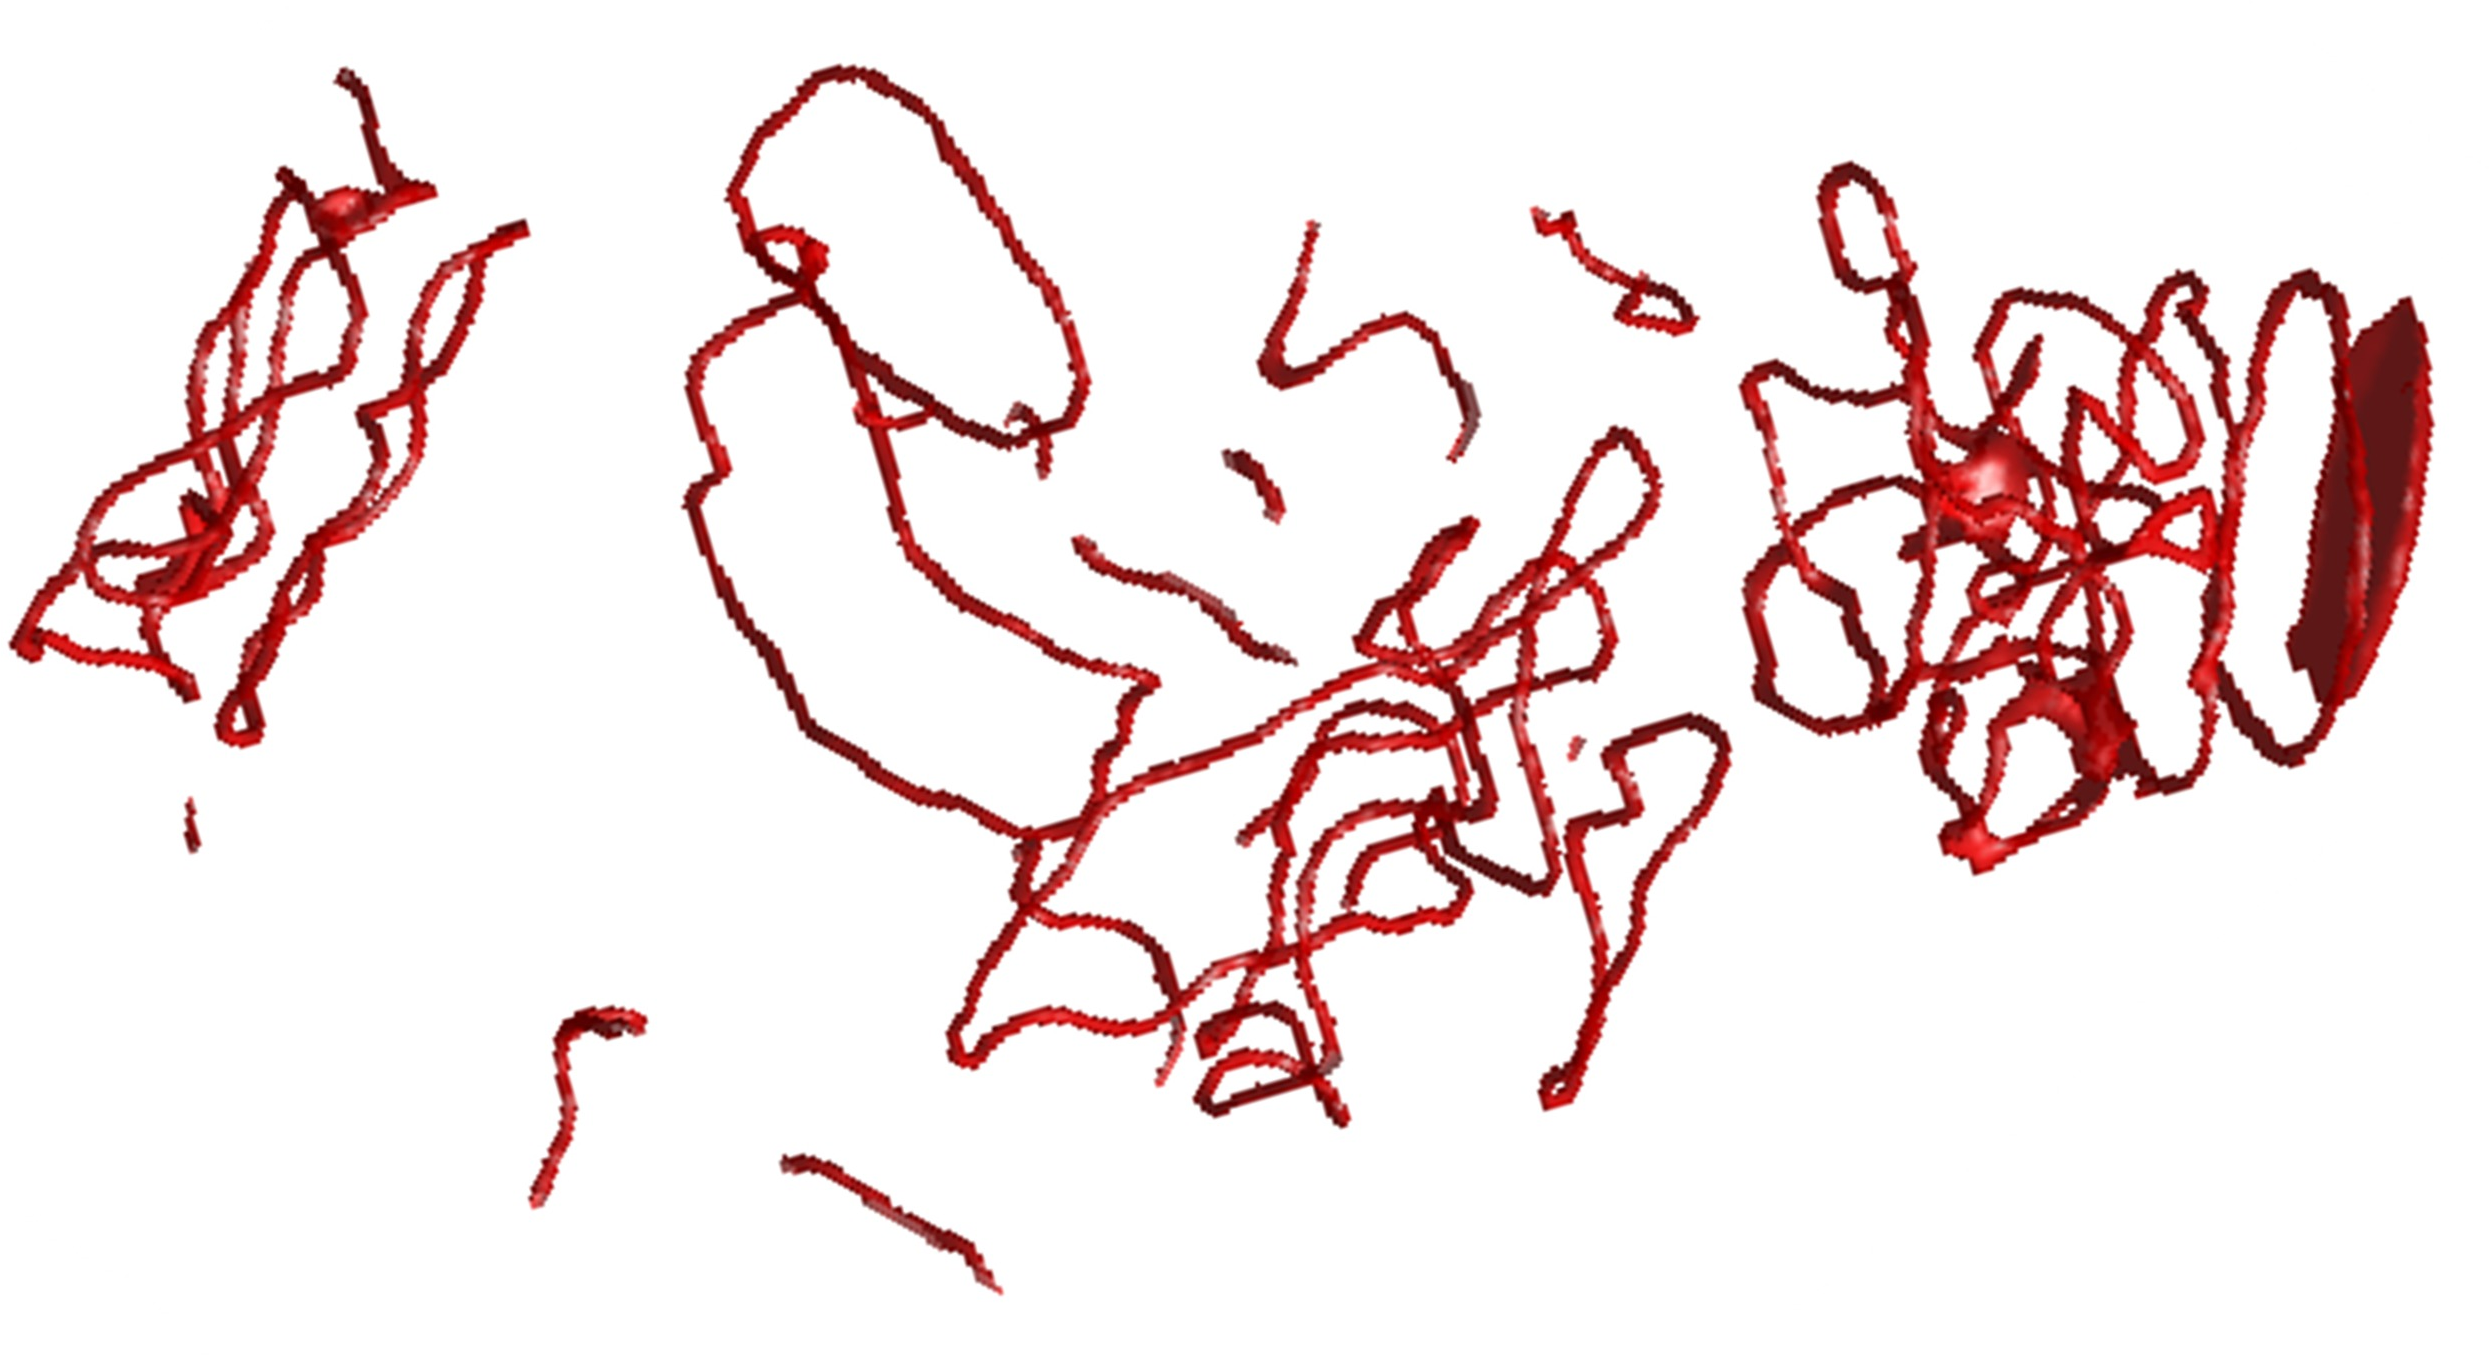
\includegraphics[width=0.9\linewidth]{wake/asymwake}
\end{minipage}%
\begin{minipage}{0.5\linewidth}%
\vspace{-0.84\baselineskip}(b)\\
\begin{tikzpicture}
  \begin{axis}[ylabel near ticks,xlabel near ticks,
      axis on top,
      width=\linewidth,
      xlabel=$x/\xi$,
      ylabel=$y/\xi$,
      unit vector ratio=1 1 1,
      xmin = -60,xmax = 100,ymin = -35,ymax = 35,
      major tick length = 0.07cm,
    ]
    \addplot graphics [xmin = -60,xmax = 100,ymin = -35,ymax = 35] {wake/asymwakeyx};
  \end{axis}
\end{tikzpicture}\\%
(c)\\%
\begin{tikzpicture}
  \begin{axis}[ylabel near ticks,xlabel near ticks,
      axis on top,
      width=\linewidth,
      xlabel=$x/\xi$,
      ylabel=$z/\xi$,
      unit vector ratio=1 1 1,
      xmin = -60,xmax = 100,ymin = -35,ymax = 35,
      major tick length = 0.07cm,
    ]
    \addplot graphics [xmin = -60,xmax = 100,ymin = -35,ymax = 35] {wake/asymwakezx};
  \end{axis}
\end{tikzpicture}%
\end{minipage}%
\caption{\label{fig:3d4} Asymmetric wake in 3D at $t=340~(\xi/c)$ for an elliptical obstacle ($d=5\xi$ and $\epsilon=5$) moving at $v=0.6\,c$. (a) Isosurface plot of low density, over a range $[-60,100]$ in $x$ and $[-25,25]$ in $y$ and $z$. (b) Vortex locations in the $xy$ plane.  (c) Vortex locations in the $xz$ plane.  In (b) and (c) red/blue denotes vortex lines with quanta of circulation $+1/-1$.}
\end{figure}

We break the cylindrical symmetry of the system by tilting the obstacle by a small angle in the $xz$ plane.  The vortex rings, illustrated in Figure \ref{fig:3d4}, now become ejected and evolve asymmetrically; Kelvin waves and reconnections occur, forming an apparently disordered tangle of vortices behind the obstacle.  Due to the manner in which symmetry is broken, the wake remains approximately symmetric in the $xy$ plane, as evident in Figure \ref{fig:3d4} (b).  However, unlike in Figure \ref{fig:3d4}, the vortices do not self organise into two clusters of alternate circulation. This is due to the vortex rings interacting, reconnecting and shifting out of the plane (which manifests in 2D as two alternate-sign vortices approaching one another).



However, in the $xz$ plane (Figure \ref{fig:3d4} (c)), symmetry is broken. Due to the relatively high frequency of vortex nucleation and relatively low flow speed, like signed vortices cluster together as they are ejected by the obstacle, much like the 2D solutions seen in earlier sections.  Downstream the tangle may shift both across or out of the plane. In 2D, although this manifests as a shift in location of the vortex clusters, the clusters largely remain rather than forming dipoles. 

\section{Conclusion}
We have shown that the motion of an obstacle in a Bose-Einstein condensate produces classical-like wakes consisting of quantum vortices of the same polarity.  This is consistently observed in both 2D and 3D scenarios.  By modifying the obstacle so that it is elliptical, which reduces the critical velocity for vortex nucleation, vortices are generated at a sufficiently high rate that they undergo strong interactions with their neighbours  (rather than being swept away). This leads to the production of classical-like wakes. Symmetric wakes resemble those observed in classical flow at low $\Rey$.  These are unstable, forming time-dependent asymmetric structures similar to the B\'enard--von K\'arm\'an vortex street of classical fluid dynamics. Vortex singularities
in the inviscid superfluid thus mimic classical vortex patterns typical of viscous flows.  The effects which we describe (dependence of the critical velocity and cluster size on the obstacle's size, velocity and ellipticity) can be experimentally studied in atomic Bose-Einstein condensates using moving laser-induced potentials. They are also relevant to the motion of objects (such as vibrating wires, grids and forks) in superfluid helium, as the obstacle's ellipticity plays a role which is analogous to rough boundaries \cite{blaz08,brad05}. This idea is explored in detail in Chapter \ref{cha:afm}.


\subsection{Further Work}
\subsubsection{A `quantum' Reynolds number}
The work in this chapter has been built upon and expanded by Reeves \emph{et. al.} \cite{reeves_2015}. The group performed many 2D simulations using circular ($\varepsilon=1$) Gaussian beams over a large parameter space of $d$ and $v$. By applying the phase unwinding algorithm described in Section \ref{section:vortexremoval} to remove vortices from the periodic flow, the group performed many simulations at efficient resolutions with a high speed GPE numerical simulation GPU/CUDA code running on a cluster of graphics cards. The large number of simulations allowed Reeves \emph{et. al.} to identify a `quantum' Reynolds number, via dynamical similarity of a hard circular cylinder in classical viscous flow and superfluid flow in the presence of a soft Gaussian obstacle.

\subsubsection{Other analogues}
Many studies of classical viscous flow have been performed over the years. Collections such as Van Dyke's {\it Album of Fluid Motion} demonstrate the wide range of flows possible with various obstacle shapes and sizes in both 2D and 3D regimes. As an example, the wakes of square (rather than circular) obstacles and recesses are shown in Figure \ref{fig:dyke-imgs}. This chapter investigated the classical-like wakes in the simplest case of a cylinder in quantum flow. It would be an extremely interesting direction for future work to attempt to experiment with the more complicated examples of classical flow patterns that exist in the literature. The idea that the behaviour of many quantum vortices collectively reproduces classical physics would suggest that perhaps other analogies of classical fluid wakes exist in the quantum fluid realm. 
\begin{figure}
\centering
    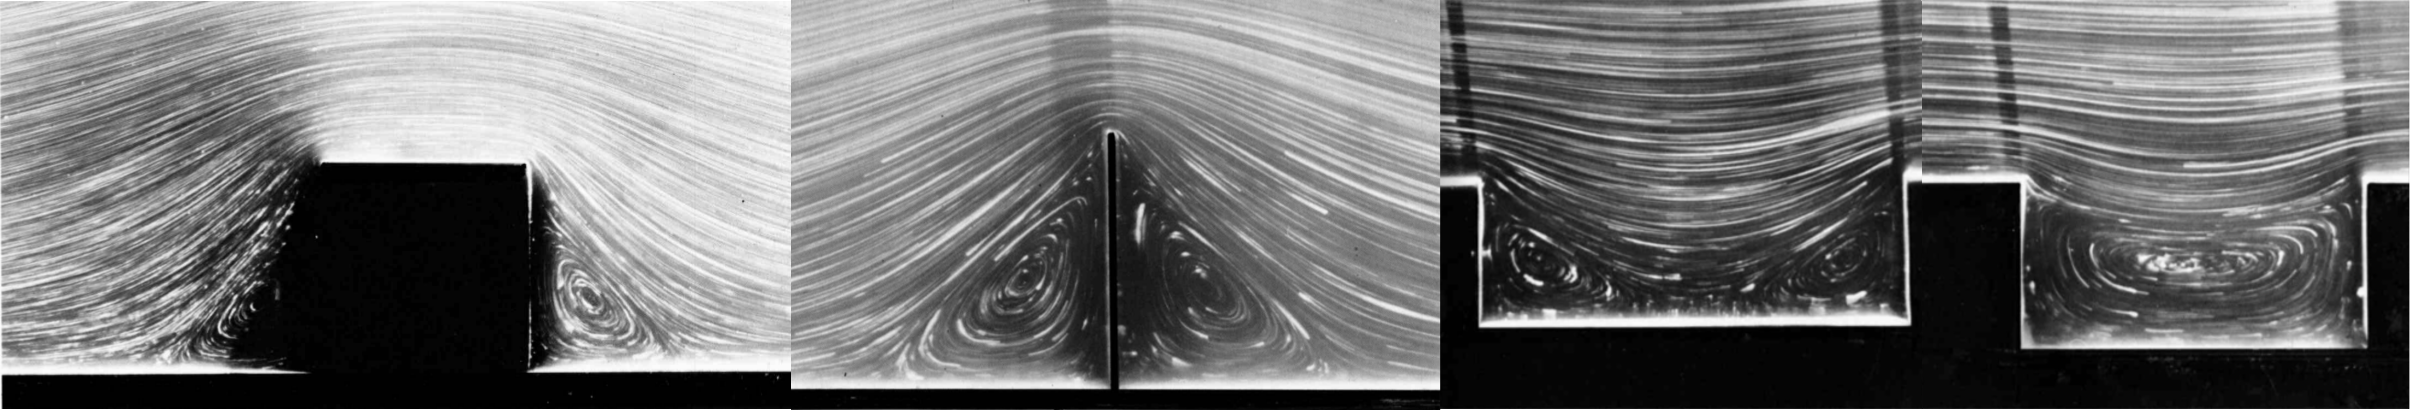
\includegraphics[width=\linewidth]{wake/square.png}
  \caption{Various examples of classical viscous fluid flow around square obstacles and recesses \cite{nagib}.} 
  \label{fig:dyke-imgs}
\end{figure}
\end{chapter}

  \begin{chapter}{\label{cha:shin}Decay of 2D quantum turbulence in a highly oblate Bose-Einstein condensate}
%%%%%%%%%%%%%%%%%%%%%%%%%%%%%%%%%%%%%%%%%%%%%
\newcommand{\gws}[1]{\textcolor{blue}{#1}}
\newcommand{\ngp}[1]{#1}%\textcolor{red}{#1}}
\newcommand{\etal}{{\it et al.}~}
\newcommand{\etalcc}{{\it et al.}}
\newcommand{\boldell}{{\mbox{\boldmath $\ell$}}}
\newcommand{\intr}{\int d \mathbf{r}}
\newcommand{\bfrt}{({\bf{r}},t)}
\newcommand{\fprt}{f({\mathbf{p}}, {\mathbf{r}},t)}

\section{Introduction}
Ultracold gaseous Bose-Einstein condensates (BECs) provide a unique testbed with which to investigate the phenomenon of quantum turbulence and the more rudimentary realm of superfluid vortex dynamics \citep{white_anderson_14,barenghi_skrbek_14}.  These systems provide an impressive degree of parameter manipulation unavailable in superfluid helium, the traditional context for studying quantum turbulence \citep{barenghi_donnelly_01}, with scope to control the particle interactions and potential landscape in both time and space.  The typical size of these systems is only one or two orders of magnitude larger than the inter-vortex spacing, which in turn is another order of magnitude larger than the vortex core size.  These compact length scales mean that the collective behaviour of vortices and their interaction with the background condensate is significant.  The emergence of turbulent-like behaviour in the form of a vortex tangle was observed by Henn {\it et al.} in 2009 by oscillating a three-dimensional condensate \cite{Henn}.  What's more, the experimentalist's handle over the confining potential enables crossover to two-dimensional quantum turbulence~\cite{parker2005}: by tightly confining the trap geometry along one axis, such that the vortices closely embody point vortices \cite{middelkamp}, states of two-dimensional quantum turbulence have been recently reported~\citep{neely_bradley_13,kwon_moon_14}.

In the recent experiment of Kwon {\it et al.} \citep{kwon_moon_14}, a trapped, oblate BEC was translated past a stationary, laser-induced obstacle.  As investigated in Chapter \ref{cha:wake}, vortices and anti-vortices were nucleated into the condensate once the relative speed exceeded a critical value~\cite{frisch92}, characteristic of superfluids. A state of two-dimensional quantum turbulence emerged, characterized by a disordered distribution of vortices.  The authors monitored the number of vortices, revealing the dependence on the relative speed and the thermal relaxation of the vortices.  They directly observed vortex collision events, characterized by a crescent-shaped depletion in the condensate density. Furthermore, some vortex cores were seen to coalesce, evidence of vortex pair annihilation.

 In this article we elucidate these experimental
findings through mean-field simulations of the two--dimensional (2D) Gross-Pitaevskii equation (GPE), both at zero-temperature and in the presence of 
thermal dissipation, modelled through a phenomenological dissipation term in 
the GPE.  Notably, our simulations provide insight into the sign of the circulation of the vortices and the early-stage evolution, not accessible experimentally.  We establish the key stages of the dynamics, from the initial nucleation of vortices and formation of a quasi-classical wake, through the rapid symmetry breaking and disorganization of the vortices, to the decay of the vortices by annihilation or passage out of the condensate.  Our approach gives excellent agreement with the experimental observations.  

\section{Model}
In the experiment, a $^{23}$Na condensate with $N=1.8\times 10^6$ atoms was confined within a highly-oblate cylindrically symmetric harmonic trap $V_{\mathrm{trap}}(x,y,z)=\frac{1}{2}m[\omega_r^2 (x^2+y^2) +\omega_z^2 z^2 ]$, with axial frequency $\omega_z=2 \pi \times 350$ Hz and radial frequency $\omega_r=2\pi \times 15$ Hz (corresponding to an aspect ratio parameter $\omega_z/\omega_r \approx 23$) and where $m$ denotes the atomic mass.  
A 2D mean-field description is strictly valid when 
the condition $N a l_z^3/l_r^3 \ll 1$ is satisfied, 
where $l_z=\sqrt{\hbar/m \omega_z}$ and $l_r=\sqrt{\hbar/m\omega_r}$ 
are the axial and radial harmonic oscillator lengths and $a$ is 
the {\it s}-wave scattering length \cite{delgado,parker2008}.  
For this experiment, $N a l_z^3/l_r^3=8.3$, i.e. the system remains 
3D in nature.   Nonetheless, the dynamics of the vortices is essentially 2D 
due to the suppression of Kelvin waves in 
the $z$-direction~\citep{jackson_proukakis_09}.  
Therefore, we will adopt a 2D description throughout this chapter and 
show that it is sufficient to capture the experimental observations.  
It is worth noting that in the $xy$ plane the condensate 
closely approximates a Thomas-Fermi (inverted parabola) density 
profile with radius $R_{\rm TF}\approx70 \mu m$.

We parametrise the condensate by the 2D wavefunction $\Psi({\bf r},t)$; the condensate density distribution follows as $n({\bf r},t)=|\Psi({\bf r},t)|^2$.  The wavefunction satisfies the GPE, Equation \ref{eq:gpe}, as described in Section \ref{section:gpe}. For computational efficiency, the numerical simulations are performed using dimensionless quantities as described in Section \ref{section:gpedimlesstrap}. Quantities are made dimensionless by writing them in terms of the harmonic oscillator units: length in terms of the radial harmonic oscillator length $l_r$, energy in terms of $\hbar\omega_r$, and time in terms of inverse radial trapping frequency $\omega_r^{-1}$. However, to remain relevant to the experimental work of Shin \etal, in this chapter we report all quantities in their full dimensional form.

We solve the GPE on a $1024 \times 1024$ grid, with grid spacing $0.27\mu$m in both $x$ and $y$, using the fourth-order Runge-Kutta method described in Section \ref{section:RK4}. We have verified that reducing the grid spacing has no effect on our results. The vortex core size is characterized by the healing length $\xi=\hbar/\sqrt{m n g}$; at the condensate centre this has the value $\xi \approx 0.6 \mu$m.

Following the experiment, the total potential acting on the condensate, $V({\bf r},t)$, is the above harmonic trap plus a static Gaussian-shaped circular obstacle potential of the form described in Section \ref{section:3dcylinderpotential},
\begin{equation}
  V_{\rm{obs}}({\bf r}) = V_0 \exp\left ( -\frac{(x-x_0)^2}{d^2}-\frac{y^2}{d^2}\right ),
\end{equation}
with $V_0=15 \mu$ and $d=11.31\mu$m.  The initial ground-state BEC is obtained by solving the GPE using the imaginary time method shown in Section \ref{section:imagTime}, with an enforced norm of $N=1.8\times 10^6$ to match the experimental value.  At $t=0$ the harmonic trap is centred at $x_0=18.5\mu$m. The trap is translated towards the left, at speed $v$, over a distance of $37 \mu$m; to smooth this speed curve we additionally include a linear acceleration/deceleration over $3.75$ms at the start/end, which is included as part of the $37\mu$m translation.  Once the trap is at rest, the obstacle amplitude $V_0$ is ramped down to zero over $0.4$s.

\section{Number of Vortices Generated}
\begin{figure}
\begin{center}
  \begin{tikzpicture}
  \begin{axis}[ylabel near ticks,xlabel near ticks,
        width=0.5\linewidth,
        xtick pos=left,
      ytick pos=left,
        xlabel=$v~(mm/s)$,
        ylabel=$N_v$,
        xmin=0.2,
        xmax=1.8,
        ymin=0,
        ymax=100,
        major tick length = 0.07cm,
        samples=300
      ]
      %\addplot+[only marks, error bars/y dir=both, error bars/y fixed=3,error bars/error bar style={thick}] file {shin/nv_v_lowtemp.dat};
      %\addplot+[only marks, error bars/y dir=both, error bars/y fixed=3,error bars/error bar style={thick},color=red,mark=square*,every mark/.append style={solid, fill=red}] file {shin/nv_v_hightemp.dat};
      \addplot+[only marks] file {shin/nv_v_lowtemp.dat};
      \addplot+[only marks,color=red,mark=square*,every mark/.append style={solid, fill=red}] file {shin/nv_v_hightemp.dat};
      \addplot+[only marks,color=black,mark size = 2, mark=diamond*,every mark/.append style={solid, fill=black}] file {shin/nv_v_exp.dat};
      \addplot+[mark=none,color=red] {(85.2084 / (1 + exp(-8.4940*x + 5.6354))-4.6183)};
      \addplot+[mark=none,color=blue] {(61.2430 / (1 + exp(-14.7576*x + 10.4699))-0.7081)};
      \addplot+[mark=none,color=black] {(64.6833 / (1 + exp(-7.8208*x + 5.5874))-2.1150)};
    \end{axis}
\end{tikzpicture}
\end{center}
\caption{\label{fig:N_vV} Number of vortices $N_v$ in the condensate after removal of the obstacle. Shown are simulations of the GPE without dissipation (red circles), with dissipation $\gamma = 0.0003$ (blue squares) and experimental results extracted from Fig.~1 of~\citep{kwon_moon_14} (black diamonds). Sigmoid fits are also shown as lines. Each point is averaged over $20$ ms once the obstacle amplitude reaches $V_0=0$.  For comparison, the speed of sound in the centre of the BEC is $v_c\approx 4.6$ mm/s.  }
\end{figure} 
Following removal of the obstacle, we determine the number of vortices in the system $N_v$ using the methods described in Section \ref{section:vortexidentifying}.  
We limit our search to $75$ percent of the Thomas-Fermi radius \ngp{(centred on the centre-of-mass to account for sloshing motion)}; by avoiding the low density periphery we avoid artefacts from ghost vortices and match closely what is performed experimentally (since vortices close to the edge are not detected due to low signal-to-noise~\citep{shin_private}). 

In Figure \ref{fig:N_vV} we plot $N_v$ versus the translation speed $v$.  We see the same {\it qualitative} form between our simulations (red circles) and the experiment (black crosses): above a critical speed $v_c \approx 0.45$mm/s vortices enter the system, nucleated by the relative motion between the obstacle and the superfluid, and for $v>v_c$ the growth in $N_v$ is initially rapid but tails off for $v\gg v_c$. Quantitatively, however, the GPE overestimates $N_v$.   One can expect that thermal dissipation, not accounted for in the GPE, will act to reduce the number of vortices in the system.

We introduce the effects of dissipation via the addition of phenomenological dissipation, $\gamma$~\citep{choi_morgan_98,tsubota_kasamatsu_02}, which enters the GPE by replacing $i$ on the left hand side by $(i-\gamma)$, a process formally derived in Section \ref{section:dgpe}.  This term induces the decay of excitations; for single vortices this manifests in them spiralling out of the trapped condensate~\citep{madarassy_barenghi_08,jackson_proukakis_09,allen_zaremba_13,yan_proukakis_14}. We choose a small value $\gamma = 0.0003$ so as to model the experiment in its very coldest realization of $\sim130$nK and enforce the norm throughout the dissipative simulations so as to emulate the experiment (for which no significant loss of atom number was observed). With this dissipation the data for $N_v$ becomes reduced, bringing it closely in line with the experimental data. Experimental limitations in resolving and counting vortices may also contribute to the over-estimate of $N_v$ from the GPE.

\section{Stages of the Condensate Evolution}

We now examine in detail the evolution of the condensate, 
charting its dynamics from the initial stage (when the
harmonic trap translation begins) to the intermediate and final stages 
(randomization and decay of the vortices).  We see the same 
qualitative evolution with and without dissipation, and for all 
velocities exceeding $v_c$.  For the purposes of illustration, 
we focus on an example with dissipation and a translation 
speed $v=1.4$mm/s. 

\begin{figure}
\centering
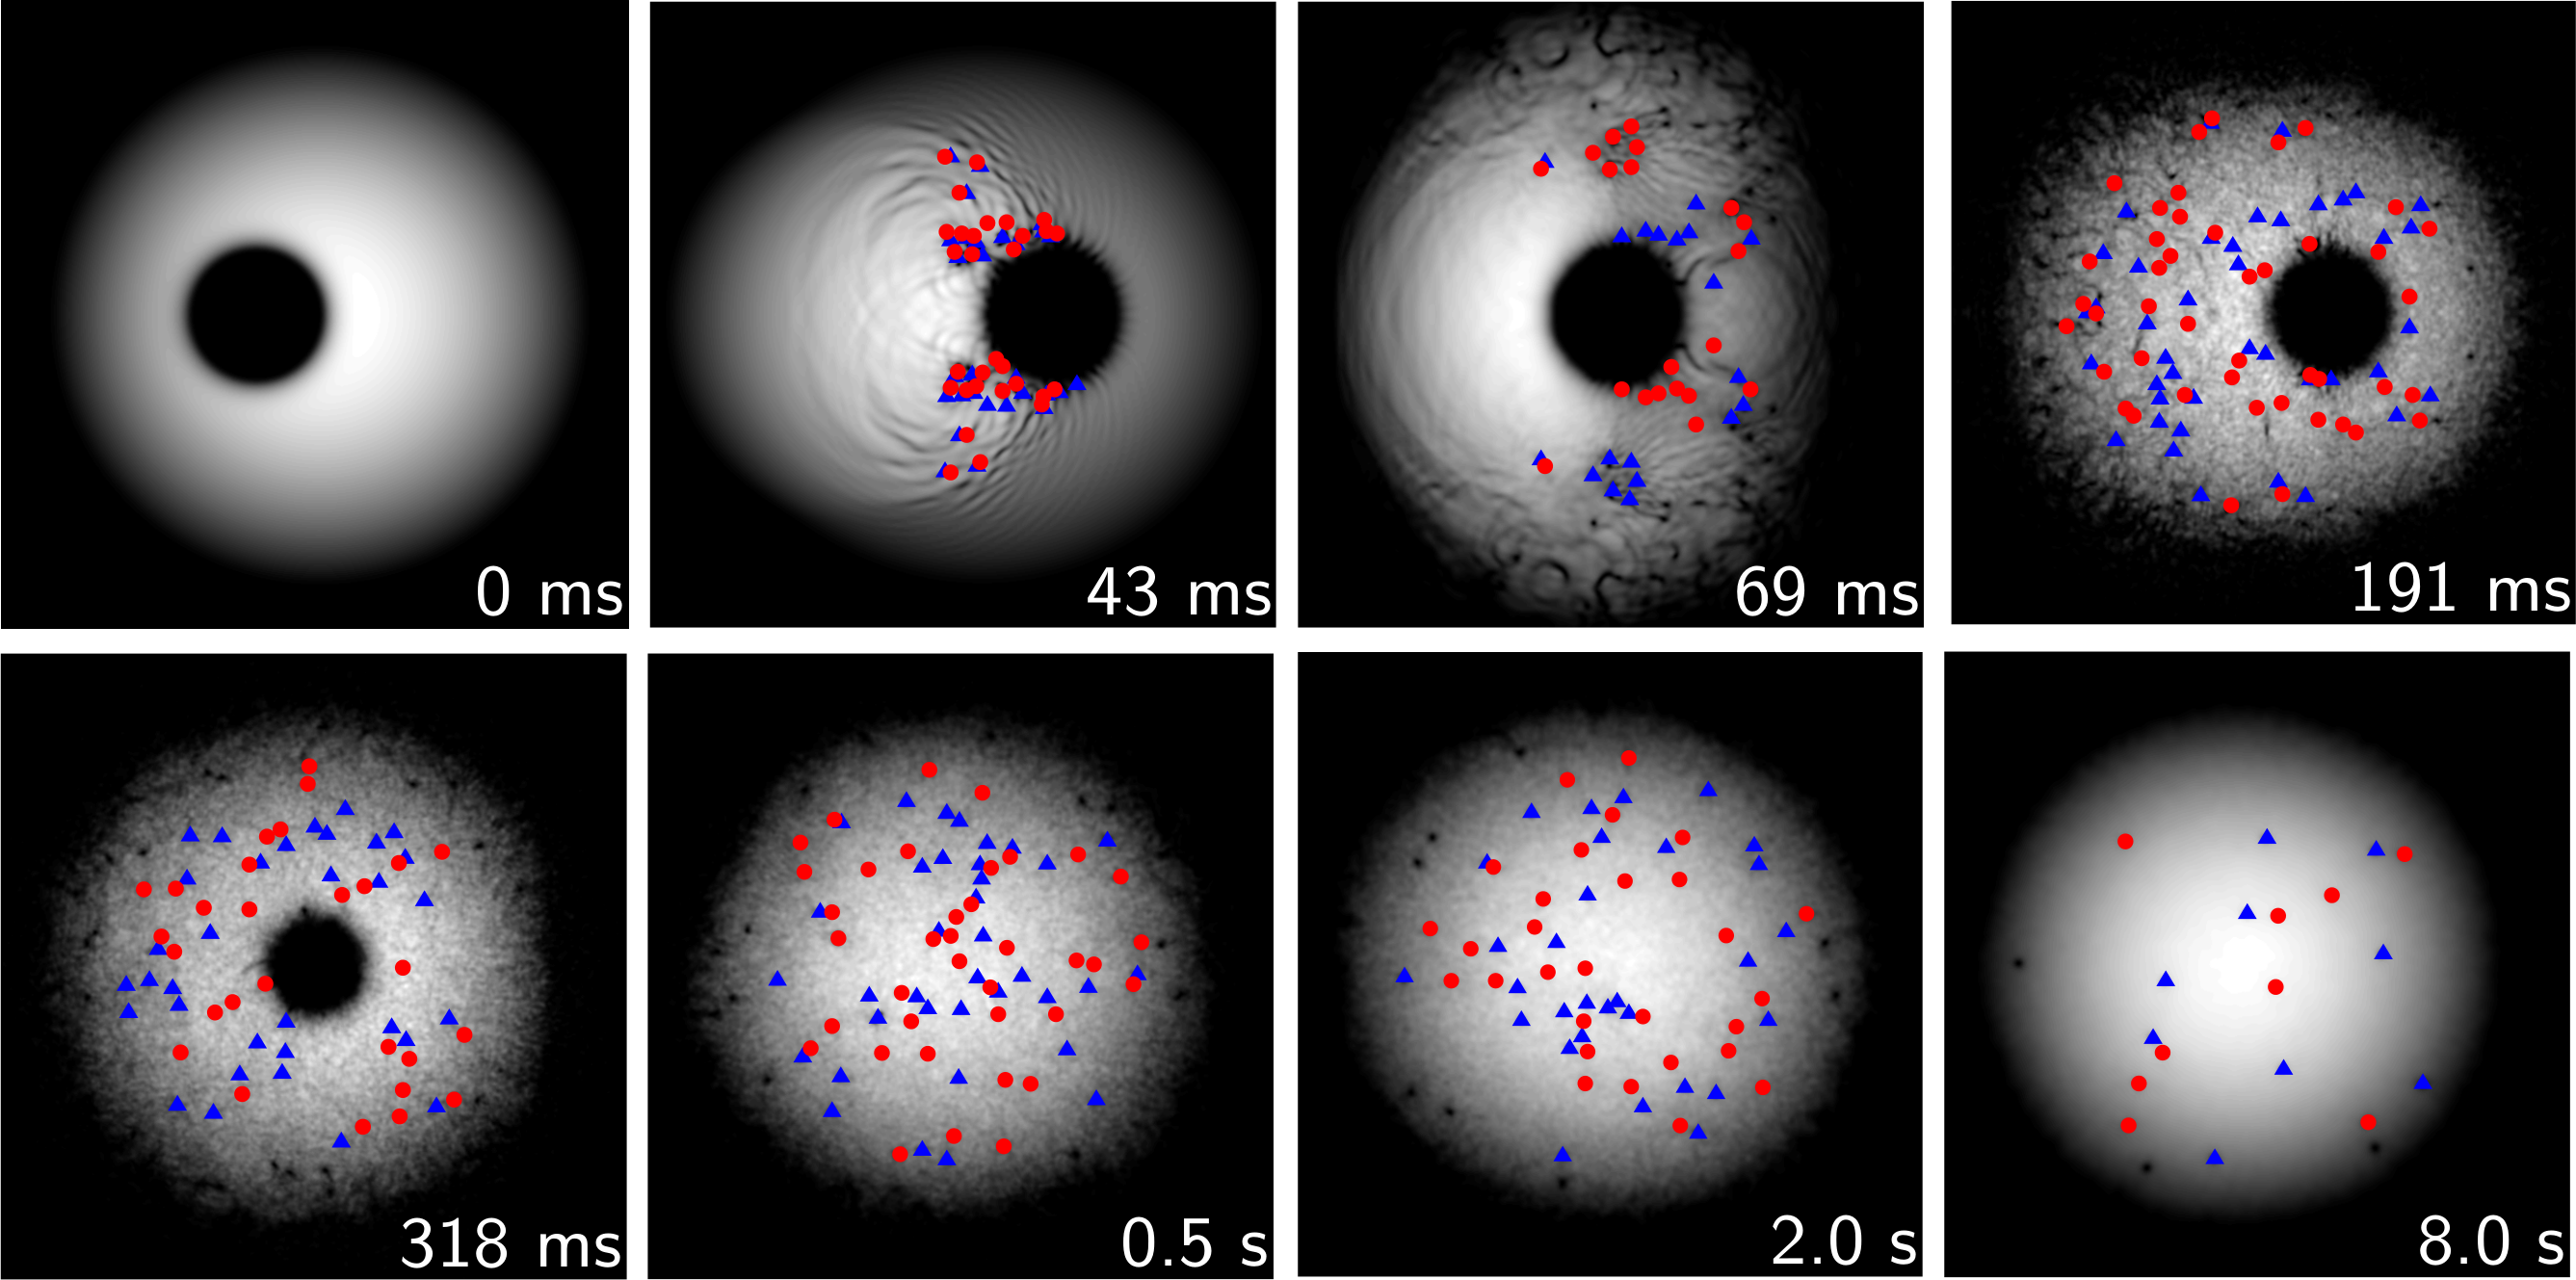
\includegraphics[width=0.95\linewidth]{shin/fig2_4x2}
\caption{\label{fig:densSnapshots} Snapshots of the condensate density, for a translational speed $v=1.4$mm/s and in the presence of dissipation ($\gamma=0.0003$). The obstacle is completely removed at $0.43$s. The field of view in each subfigure is of size $[170\mu$m$]^2$ and shifted along the $x$-axis so as to best display the condensate.  Vortices with positive (negative) circulation are highlighted by red circles (blue triangles).
}
\end{figure}

Figure \ref{fig:densSnapshots} shows the condensate density at various times. At the start of the simulation ($t=0$) the condensate has a smooth circular density profile, with a density depression due to the obstacle.  Later vortices appear as small dots of low density; superimposed red/blue markers tag vortices of positive/negative circulation.

\subsection{Vortex Nucleation and Wake Formation}

To initiate the dynamics, the harmonic t1rap is translated to the left.  This is performed sufficiently rapidly that the condensate does not adiabatically follow the trap minimum, but rather begins a sloshing motion in the trap; the centre-of-mass of the BEC oscillates at the trap frequency and the BEC undergoes a quadrupolar shape oscillation. As the BEC sloshes first to the left, its speed increases.  When the local fluid velocity exceeds the speed of sound, vortices nucleate \cite{frisch92} at the poles of the obstacle
(where the local fluid velocity is the greatest) 
and are washed downstream (to the left).  
As seen in Chapter \ref{cha:wake}, the pattern of vortices nucleated by a moving obstacle 
in a superfluid depends, in general, on the  speed, shape and size of 
the obstacle~\citep{jma00,saito10,stagg_parker_14}. 
During the initial evolution vortices of negative
and positive circulation are created near each pole in an 
irregular manner, sometimes with alternating circulation;  
other times several vortices of the same circulation appear.  
In our case, the rate of vortex nucleation is sufficiently 
high that the vortices interact strongly with each other, 
collectively forming macroscopic clusters of negative and positive 
vortices downstream of the object ($t=43$ms).  This is reminiscent of the wakes in classical viscous fluids past cylindrical obstacles \cite{stagg_parker_14}.  
During this early stage, vortices of opposite 
circulation may become very close and annihilate (i.e. undergo 
a 2D reconnection), leaving behind density (sound) waves. The condensate then sloshes to the right; this 
motion not only carries the existing vortices to the opposite 
(right) side of the obstacle but nucleates further vortices. 
As the condensate's sloshing mode is damped by 
the dissipation, the relative speed of the obstacle decreases
and the vortex nucleation pattern changes: 
like-signed vortices are generated near each pole, 
forming symmetric classical--like wakes~\cite{stagg_parker_14}. 
This effect leads to further clustering of like-signed vortices   
($t=69$ms). As the condensate continues to slosh, more
vortices nucleate into the system. It must be stressed that,
up to these early times ($t=191$ms), the vortex distribution remains symmetric 
about the $x$ axis.

Without the dissipation term in the GPE, the sloshing mode initially decays while the obstacle is present but then persists with constant amplitude once the obstacle is removed.  If dissipation is included then the sloshing mode continues to decay. Figure \ref{fig:com_slosh} shows the centre-of-mass oscillation over time, demonstrating the decay and that in either case, the sloshing mode is produced at the trap frequency.
\begin{figure}
\begin{center}
  \begin{tikzpicture}
  \begin{axis}[ylabel near ticks,xlabel near ticks,
        width=0.5\linewidth,
        xtick pos=left,
        ytick pos=left,
        xlabel={Time (s)},
        ylabel={Centre-of-mass ($\mu$m)},
        xmin=0,
        xmax=1.9,
        major tick length = 0.07cm
      ]
      %\addplot+[mark=none,color=red] {(85.2084 / (1 + exp(-8.4940*x + 5.6354))-4.6183)};
      \addplot+[mark=none,color=blue,thick] file {shin/com_gpe.dat};
      \addplot+[mark=none,color=red,thick] file {shin/com_dgpe.dat};
    \end{axis}
\end{tikzpicture}
\end{center}
\caption{\label{fig:com_slosh} Centre-of-mass oscillations during condensate evolution for the BEC without the dissipation term (blue), and with a dissipation of $\gamma = 0.0003$ (red).}
\end{figure} 

\subsection{Vortex Randomization}
In the presence of the obstacle and the sloshing mode,
vortices continually nucleate and their spatial distribution remains
approximately symmetric about the $x$ axis.  
At later times ($t>318$ms) this symmetry breaks and the vortices 
evolve into a completely disorganised, apparently random 
configuration with no significant clustering of like-signed vortices.  \ngp{This random distribution of vortices is consistent with the experimental observations \cite{kwon_moon_14}; following this we also classify the system as one of quantum turbulence.
Besides vortices, the condensate contains also collective modes and
an energetic, disordered sound field, with this spatial range of excitations further indicative of two-dimensional 
quantum turbulence \cite{parker2005,neely_bradley_13}. (Note that the typical characteristic diagnostics of steady-state 2D quantum turbulence, e.g. power-law energy spectra and the inverse energy cascade, are not appropriate here since the system is not continuously driven and does not reach steady state.)}

\ngp{The vortex randomization is driven by the growth of numerical noise.  We have repeated our results in the presence of imposed noise (amplitude $5\%$, as described elsewhere \cite{stagg_parker_14}) and find the qualitative dynamics to be unchanged (although, as one would expect, the vortex randomization occurs at a slightly earlier time).  This noise serves to model the natural fluctuations that arises in a realistic experimental scenario, e.g. due to thermal and quantum atomic fluctuations, electromagnetic noise, vibrations, etc.}

It is interesting to note the obstacle is still in the system 
at this point, nucleating vortices in a symmetrical manner. 
The disorganised vortices already in the system create a velocity 
field which quickly mixes newly created vortices nucleated at the
poles of the obstacle. Visual inspection, confirmed by the RCA clustering-detection algorithm~\citep{white12,reeves_billam_13} described in Section \ref{section:reevesalgorithm}, 
shows no significant clusters beyond this stage of the evolution. 
By the time the obstacle is removed the vortex configuration is 
essentially random, but 
the number of positive and negative vortices stays approximately equal.
It is important to remark that, without detecting the sign of the vortex circulation, we
could not reach these conclusions.

\begin{figure}
\begin{center}
  \begin{tikzpicture}
  \begin{axis}[ylabel near ticks,xlabel near ticks,
        width=0.5\linewidth,
        xtick pos=left,
        ytick pos=left,
        xlabel={Time (s)},
        ylabel=$N_v$,
        xmin=0,
        xmax=0.5,
        ymin=0,
        ymax=90,
        major tick length = 0.07cm
      ]
      \addplot+[mark=none,color=blue,thick] file {shin/nv_t_lowtemp.dat};
      \addplot+[mark=none,color=red,thick] file {shin/nv_t_hightemp.dat};
    \end{axis}
\end{tikzpicture}
\end{center}
\caption{\label{fig:N_vTime} Growth of vortex number (in a single realization) at early times for a translational speed of $v=1.4$mm/s. Shown are the results with no dissipation (blue) and with dissipation $\gamma=0.0003$ (red).}
\end{figure}

\subsection{Vortex Decay}
It is clear from Figure \ref{fig:densSnapshots} that, following the removal 
of the obstacle, the number of vortices, $N_v$, depletes.   
Indeed, one expects that the condensate will decay towards its 
vortex--free, time--independent ground state.  To quantify the vortex generation and
decay, Figure \ref{fig:N_vTime} plots the growth of $N_v$ at early times, 
and Figure \ref{fig:N_vLong} (a, b) plots the decay of vortices over the entire experimental time period. 
The onset of vortex nucleation is at around $t=0.02$ms; 
this is the time taken for accelerating condensate to exceed the speed of 
sound at the poles of the object.
At first $N_v$ grows steeply, as vortices (around 40-60) are rapidly driven into the system. Subsequently, $N_v$ grows more slowly; vortices continue to be nucleated from the obstacle but vortices undergo annihilation or move into low density regions where they are not detected.  The fluctuations in $N_v$ are amplified, particularly at early times, by the shape oscillations of the condensate, which carry vortices in and out of the detection radius. As the obstacle is removed, the surrounding condensate fills the low density area. Vortices (including some outside of the detection radius) move inwards with the condensate, causing $N_v$ to peak at $t\approx 0.4$s.
\begin{figure}
\begin{center}
  \begin{tikzpicture}
  \begin{axis}[ylabel near ticks,xlabel near ticks,
        width=0.45\linewidth,
        xtick pos=left,
        ytick pos=left,
        xlabel={Time (s)},
        ylabel=$N_v$,
        xmin=0.45,
        xmax=8,
        ymin=0,
        ymax=82,
        axis on top,
        major tick length = 0.07cm
      ]
      \addplot [thick,color=red,mark=none,draw=none,fill=red!60]coordinates {(100, 100) (100, 0) (0, 0) (0, 100)};
      \addplot[mark=none,draw=none,thick,fill=cyan!70] file {shin/nv_t_a_split.dat}\closedcycle;
      \addplot[mark=none,color=black,thick,fill=white] file {shin/nv_t_a_lower.dat}\closedcycle;
      \node[anchor=west] at (axis cs:  1.25,  77) {\sf Drift};
      \node[anchor=west] at (axis cs:  1.25,  55) {\sf Annihilation};
    \end{axis}
\end{tikzpicture}
\begin{tikzpicture}
  \begin{axis}[ylabel near ticks,xlabel near ticks,
        width=0.45\linewidth,
        xtick pos=left,
        ytick pos=left,
        xlabel={Time (s)},
        ylabel=$N_v$,
        xmin=0.45,
        xmax=8,
        ymin=0,
        ymax=64,
        axis on top,
        major tick length = 0.07cm
      ]
      \addplot [thick,color=red,mark=none,draw=none,fill=red!60]coordinates {(100, 100) (100, 0) (0, 0) (0, 100)};
      \addplot[mark=none,draw=none,thick,fill=cyan!70] file {shin/nv_t_b_split.dat}\closedcycle;
      \addplot[mark=none,color=black,thick,fill=white] file {shin/nv_t_b_lower.dat}\closedcycle;
      \node[anchor=west] at (axis cs:  2,  58) {\sf Drift};
      \node[anchor=west] at (axis cs:  2,  40) {\sf Annihilation};
    \end{axis}
\end{tikzpicture}\\%
\begin{tikzpicture}
  \begin{axis}[ylabel near ticks,xlabel near ticks,
        width=0.45\linewidth,
        xtick pos=left,
        ytick pos=left,
        xlabel={Time (s)},
        ylabel={\# Vortices Removed},
        xmin=0.45,
        xmax=8,
        ymin=0,
        ymax=61,
        axis on top,
        major tick length = 0.07cm
      ]
      \addplot[mark=none,color=red] file {shin/nv_t_c_drift.dat};
      \addplot[mark=none,color=blue] file {shin/nv_t_c_an.dat};
      \addplot[mark=none,color=red,ultra thick,dashed] file {shin/nv_t_c_drift_fit.dat};
      \addplot[mark=none,color=blue,ultra thick,dashed] file {shin/nv_t_c_an_fit.dat};
    \end{axis}
\end{tikzpicture}%
\begin{tikzpicture}
  \begin{axis}[ylabel near ticks,xlabel near ticks,
        width=0.45\linewidth,
        xtick pos=left,
        ytick pos=left,
        xlabel={Time (s)},
        ylabel={\# Vortices Removed},
        xmin=0.45,
        xmax=8,
        ymin=0,
        ymax=32,
        axis on top,
        major tick length = 0.07cm
      ]
      \addplot[mark=none,color=red] file {shin/nv_t_d_drift.dat};
      \addplot[mark=none,color=blue] file {shin/nv_t_d_an.dat};
      \addplot[mark=none,color=red,ultra thick,dashed] file {shin/nv_t_d_drift_fit.dat};
      \addplot[mark=none,color=blue,ultra thick,dashed] file {shin/nv_t_d_an_fit.dat};
    \end{axis}
\end{tikzpicture}%
\end{center}
\caption{\label{fig:N_vLong} Vortex decay in the absence of dissipation (a, c) and with dissipation $\gamma=0.0003$ (b, d) for a translational speed of $v=1.4$mm/s.  The upper figures show the decay of the total vortex number $N_v(t)$, with the contribution of drifting and annihilation depicted by the shaded regions.  The lower figures show the drift number $N_d(t)$ and annihilation number $N_a(t)$, plus their respective fits.}
\end{figure}

\ngp{ Following removal of the obstacle, the vortex number $N_v$ decays with time.  This is shown in Figure \ref{fig:N_vLong}(a) and (b) for the absence and presence of dissipation, respectively. }  Kwon {\etal}~\citep{kwon_moon_14} argued that there are two mechanisms 
by which vortices decay: (i) thermal dissipation
(resulting in drifting of vortices to the edge of the condensate),
and (ii) vortex-antivortex annihilation events, and proposed
that the vortex decay takes the form:
\begin{equation}
\frac{{\rm d}N_v}{{\rm d}t}= - \Gamma_1 N_v - \Gamma_2 N_v^2.
\label{eqn:N_v_decay}
\end{equation}
Here the linear and nonlinear terms, parametrised by the positive
coefficients $\Gamma_1$ and $\Gamma_2$, respectively, model
these two decay processes.  From our simulations we are able to independently count the number of vortices which drift out and the number which annihilate.  
We decompose the number of vortices according to 
\begin{equation}
  N_v(t) = N_i - N_d(t) - N_a(t),
\label{eqn:N_v_decomp}
\end{equation}
where $N_i$ is the initial number of vortices (when the obstacle is removed), $N_d(t)$ is the cumulative number of vortices which have drifted out of the condensate and $N_a(t)$ is the cumulative number which have undergone pair annihilation.
The contribution of both vortex drifting and annihilation to the overall decay of $N_v$ is depicted by the coloured regions in Figure \ref{fig:N_vLong}(a) and (b).  In the absence of dissipation  the vortex decay is dominated by annihilation.  Indeed, apart from at early times (where internal condensate dynamics carry vortices out to high radii), no vortices drift out.  In contrast, in the presence of dissipation, vortices continue to drift out over time, consistent with dissipative dynamics of single vortices \citep{allen_zaremba_13}.

Unfortunately, fitting $N_v(t)$ directly to Equation (\ref{eqn:N_v_decay}) leads to inconclusive results. While we find that the best-fitting solutions fit the data well, the resulting values for $\Gamma_1$ are found to be negative, corresponding to a positive growth. Considering that $\Gamma_1$ is a term associated to thermal dissipation there is no reason to expect a growth here. We interpret this inconsistency as resulting from fitting Equation (\ref{eqn:N_v_decay}) directly; the meaning of the rates $\Gamma_1$ and $\Gamma_2$ (i.e as characterising rates of vortex loss through drifting and vortex-antivortex annihilation) are not enforced, and so the best-fit parameters cannot be used to infer anything about the physical processes.

Our solution is to enforce the meaning of $\Gamma_1$ and $\Gamma_2$ while performing the fitting process. The decomposition of $N_v$ as Equation (\ref{eqn:N_v_decomp}) enables us to independently fit the drift and annihilation decay processes as two coupled ODEs for $N_d$ and $N_a$,
\begin{equation}
  \frac{{\rm d}N_d}{{\rm d}t} = \Gamma_1 N_v,~~~~~~~~~~~~~~
  \frac{{\rm d}N_a}{{\rm d}t} = \Gamma_2 N_v^2.
\label{eqn:N_v_couple}
\end{equation}
By taking the time derivative of Equation (\ref{eqn:N_v_decomp}) and substituting in Equation (\ref{eqn:N_v_couple}), Equation (\ref{eqn:N_v_decay}) can be recovered. As a consequence of fitting the coupled ODEs independently, the physical meaning of each rate term is enforced. To further fix the physical meaning, the fitted value of both $\Gamma_1$ and $\Gamma_2$ are forced to be positive (corresponding to a vortex decay over time). The vortex decomposition along with the each independent fit is shown in Figure \ref{fig:N_vLong}(c) and (d) for the absence and presence of dissipation, respectively. We find that the rate equation fits fairly well most cases, although finds difficulty in fitting the lack of vortex decay via drifting when $\gamma=0$.

In the absence of dissipation, we find $\Gamma_{2} = 0.0040$. While the experimental observations \cite{kwon_moon_14} suggest $\Gamma_2$ is proportional to $T^2$ and thus approaches 0 as $T\rightarrow0$, our results demonstrate a finite $\Gamma_2$ in this limit. We also find a corresponding value of $\Gamma_{1} = 0$ in the absence of dissipation. However, it is not appropriate to discuss the physical meaning of $\Gamma_1$ in this case, since $\gamma=0$ and so $N_d$ is not of a decaying form; this also explains the less successful fit for $N_d$ in the absence of dissipation.

With the inclusion of a dissipation of $\gamma=0.0003$ we obtain $\Gamma_{1} = 0.093$ and $\Gamma_{2} = 0.0041$, which are comparable to the coldest experiments of Kwon \etal We find a negligible modification to the rate of vortex decay due to annihilation, but an increase to the rate of vortex decay via the drifting out mechanism, as expected when introducing dissipation into the system \citep{allen_zaremba_13}.

%\begin{figure}
%\centering
%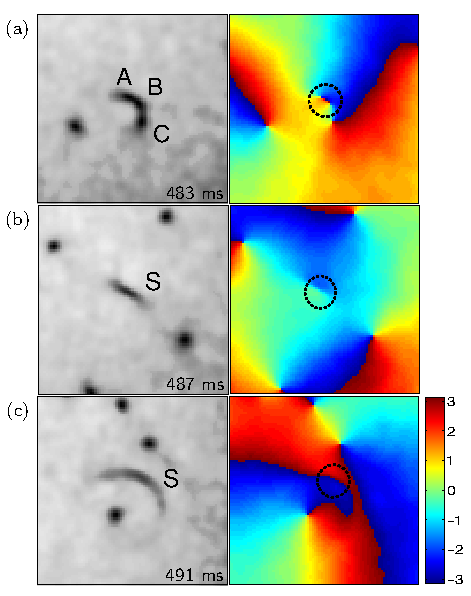
\includegraphics[width=0.9\linewidth]{shin/fig5}
%\caption{\label{fig:cresentPlots} Density (left) and phase (right) just before (a), immediately following (b) and a later time after (c) a vortex-antivortex annihilation event.  The field of view is  $[23.5\mu$m]$^2$, centered on the vortex pair/sound pulse (highlighted by a circle in the phase).}
%\end{figure}
\begin{figure}
\hspace*{0.07\linewidth}(a)\hspace{0.23\linewidth}(b)\hspace{0.23\linewidth}(c)\\
\hspace*{0.05\linewidth}\begin{tikzpicture}
  \begin{axis}[ylabel near ticks,xlabel near ticks,
      width=0.35\linewidth,
      height=0.35\linewidth,
      axis on top,
      xmin=-10,
      xmax=10,
      xlabel={},
      xticklabels={,,},
      ymin=-10,
      ymax=10,
      ylabel={},
      yticklabels={,,},
      major tick length = 0.00cm,
      minor tick length = 0.00cm
      ]
      \addplot graphics [xmin=-10,xmax=10,ymin=-10,ymax=10] {shin/fig5_d1.png};
      \node at (axis cs:  -1,  4) {{\sf A}};
      \node at (axis cs:  2,  2) {{\sf B}};
      \node at (axis cs:  3,  -2) {{\sf C}};
      \node[anchor=south east] at (axis cs:  10,  -10) {{\sf 483 ms}};
    \end{axis}
\end{tikzpicture}\hspace{-0.5cm}
\begin{tikzpicture}
\begin{axis}[ylabel near ticks,xlabel near ticks,
      width=0.35\linewidth,
      height=0.35\linewidth,
      axis on top,
      xmin=-10,
      xmax=10,
      xlabel={},
      xticklabels={,,},
      ymin=-10,
      ymax=10,
      ylabel={},
      yticklabels={,,},
      major tick length = 0.00cm,
      minor tick length = 0.00cm
      ]
      \addplot graphics [xmin=-10,xmax=10,ymin=-10,ymax=10] {shin/fig5_d2.png};
      \node at (axis cs:  1,  3) {{\sf S}};
      \node[anchor=south east] at (axis cs:  10,  -10) {{\sf 487 ms}};
    \end{axis}
\end{tikzpicture}\hspace{-0.5cm}
\begin{tikzpicture}
\begin{axis}[ylabel near ticks,xlabel near ticks,
      width=0.35\linewidth,
      height=0.35\linewidth,
      axis on top,
      xmin=-10,
      xmax=10,
      xlabel={},
      xticklabels={,,},
      ymin=-10,
      ymax=10,
      ylabel={},
      yticklabels={,,},
      major tick length = 0.00cm,
      minor tick length = 0.00cm
      ]
      \addplot graphics [xmin=-10,xmax=10,ymin=-10,ymax=10] {shin/fig5_d3.png};
      \node at (axis cs:  3,  2) {{\sf S}};
      \node[anchor=south east] at (axis cs:  10,  -10) {{\sf 491 ms}};
    \end{axis}
\end{tikzpicture}\vspace{-1.1cm}\\
\hspace*{0.05\linewidth}\begin{tikzpicture}
  \begin{axis}[ylabel near ticks,xlabel near ticks,
      width=0.35\linewidth,
      height=0.35\linewidth,
      axis on top,
      xmin=-10,
      xmax=10,
      xlabel={},
      xticklabels={,,},
      ymin=-10,
      ymax=10,
      ylabel={},
      yticklabels={,,},
      major tick length = 0.00cm,
      minor tick length = 0.00cm
      ]
      \addplot graphics [xmin=-10,xmax=10,ymin=-10,ymax=10] {shin/fig5_p1_c1.png};
      \draw[black,ultra thick,dashed] (axis cs: 0.2,1) circle (1.7);
    \end{axis}
\end{tikzpicture}\hspace{-0.5cm}
\begin{tikzpicture}
\begin{axis}[ylabel near ticks,xlabel near ticks,
      width=0.35\linewidth,
      height=0.35\linewidth,
      axis on top,
      xmin=-10,
      xmax=10,
      xlabel={},
      xticklabels={,,},
      ymin=-10,
      ymax=10,
      ylabel={},
      yticklabels={,,},
      major tick length = 0.00cm,
      minor tick length = 0.00cm
      ]
      \addplot graphics [xmin=-10,xmax=10,ymin=-10,ymax=10] {shin/fig5_p2_c1.png};
      \draw[black,ultra thick,dashed] (axis cs: -1,1) circle (1.7);
    \end{axis}
\end{tikzpicture}\hspace{-0.5cm}
\begin{tikzpicture}
\begin{axis}[ylabel near ticks,xlabel near ticks,
      width=0.35\linewidth,
      height=0.35\linewidth,
      axis on top,
      xmin=-10,
      xmax=10,
      xlabel={},
      xticklabels={,,},
      ymin=-10,
      ymax=10,
      ylabel={},
      yticklabels={,,},
      major tick length = 0.00cm,
      minor tick length = 0.00cm,
      colorbar style={title={Phase},text width=0.5em,major tick length = 0.07cm},
      point meta min = -3.141592,
      point meta max = 3.141592,
      colorbar,colormap name=hsvcl
      ]
      \addplot graphics [xmin=-10,xmax=10,ymin=-10,ymax=10] {shin/fig5_p3_c1.png};
      \draw[black,ultra thick,dashed] (axis cs: 0.5,1.5) circle (1.7);
    \end{axis}
\end{tikzpicture}
\caption{\label{fig:cresentPlots} Density (upper) and phase (lower) just before (a), immediately following (b) and a later time after (c) a vortex-antivortex annihilation event.  The field of view is  $[23.5\mu$m]$^2$, surrounding the vortex pair/sound pulse (highlighted by a circle in the phase).}
\end{figure}


\section{Crescent-Shaped Density Structures}
In the experiment, Kwon {\etal}observed the occasional appearance of crescent-shaped waves of 
depleted density.  Lacking direct access to the vortex signs,
they suggested that these structures result from
annihilation events of vortices of opposite 
circulation~\citep{nazarenko_onorato_07,rorai_skreenivasan_12,prabhakar_singh_13}: a vortex reconnection is predicted to 
induce an intense, localised, rarefaction 
sound pulse~\cite{leadbeater,zuccher}.  
Figure~\ref{fig:cresentPlots} shows snapshots of the condensate density 
and phase during a reconnection event. Vortices show up as localized dips 
in the density (upper row) and $2 \pi$-defects in the phase (lower row). 
Figure~\ref{fig:cresentPlots} (a) shows a vortex (A) and antivortex (B) 
close to each other, and a third vortex (C) in the vicinity.
Note that the individual vortices are not spatially resolvable 
through their density alone (the vortex cores merge into a deep, elongated 
crescent-shaped depression), but they are clearly identified by the 
phase plot.  A short time later (b), vortices A and B annihilate, 
as confirmed by the disappearance of their phase singularities, 
leaving behind a shallow rarefaction pulse (S) with a linear phase step.  
This pulse rapidly evolves into a shallow, 
crescent-shaped sound wave [Figure \ref{fig:cresentPlots} (c)].  
\ngp{In other words, our simulations yield crescent-shaped density features 
as seen in the experiment, but these features are not uniquely formed 
by annihilation events - they may also result from from two (or more) 
vortices in close proximity.  Information about the condensate phase 
is thus crucial to distinguish the nature
of these observed structures.  In this direction, an approach has recently been proposed for the experimental detection of quantized vortices and their circulation in a 2D BEC \cite{powis}.}

\section{Vortex Generation via an Elliptical Obstacle}
It is evident from the snapshots in Figure 2 that the initial translation of the condensate past the obstacle generates not just vortices but also shape excitations, sound waves (low-amplitude density waves), and high-amplitude density waves.  These additional excitations will heat the condensate and modify the subsequent turbulent dynamics in a highly nonlinear and complicated manner.  While reducing the translational speed reduces this disruption, this also reduces the number of vortices.  A less disruptive and more efficient (higher rate of vortex nucleation) means to generate vortices may be provided by employing a laser-induced obstacle of a form similar to that used in Chapter \ref{cha:wake}, with an {\it elliptical} rather than circular cross-section (experimentally attainable through cylindrical beam focusing).

Repeating our simulations with such an elliptical obstacle, governed by Equation (\ref{eq:potentialcylinder}), with arbitrary ellipticity $\epsilon=3$ (the short/long axis being parallel/perpendicular to the flow) confirms the same qualitative behaviour as in Chapter \ref{cha:wake} for homogeneous systems \citep{stagg_parker_14}: the ellipticity acts to reduce the critical superfluid velocity and, for a given flow speed, increase the rate of vortex nucleation. To illustrate the merits of the elliptical obstacle, in Figure \ref{fig:ellipse} we depict snapshots of the condensate dynamics for ellipticity $\epsilon=3$ and a translational speed of $v=0.8$mm/s. Despite a lower translational speed, the number of vortices generated by the time the obstacle is removed is almost identical to the circular example of Figure \ref{fig:N_vTime}.  As a consequence of the reduced translational speed, the condensate disruption is visibly reduced. It is also worth noting that the elliptical obstacle promotes the formation of clusters of like-signed vortices (see intermediate time), and thus may facilitate future exploration of coherent vortex structures.


\begin{figure}
\centering
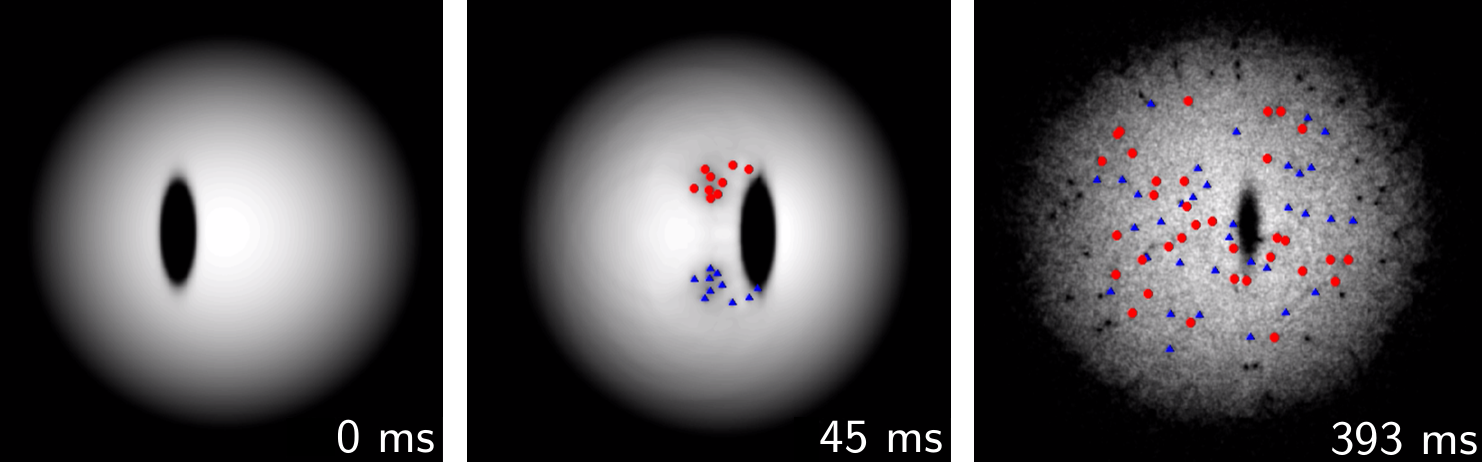
\includegraphics[width=0.9\linewidth]{shin/fig6.png}
\caption{\label{fig:ellipse} Snapshots of the condensate density for a translational of speed $v=0.8$mm/s past an elliptical obstacle (ellipticity $\epsilon=3$). The field of view in each subfigure is of size $[170\mu$m$]^2$ and shifted along the $x$-axis so as to best display the condensate.  Compared to the corresponding snapshots in Figure 2, the elliptical obstacle generates as many final vortices but at a lower translational speed and with reduced condensate disruption.
}
\end{figure}
\section{Conclusions}
In conclusion, we have shown that the recent experimental creation and decay of vortices within a BEC~\citep{kwon_moon_14} is well described by simulations of the 2D GPE with phenomenological dissipation (despite the 3D nature of the system).  Theoretical access to the condensate phase, and thus the circulation of the vortices, promotes our understanding of the dynamics.  In the early stages of 
translation of the obstacle, a quasi-classical wake of vortices 
forms behind it, before symmetry breaking causes disorganisation 
of the vortices.  After the obstacle is removed, 
the vortices decay in a manner which is consistent with the two mechanisms proposed by 
Kwon \etalcc, i.e. loss of vortices at the condensate edge due to thermal dissipation and vortex-antivortex 
annihilation events within the condensate. 
We confirm the occasional appearance of 
crescent-shaped density features, resulting either from the proximity 
of vortex cores or from a sound pulse which follows a 
vortex-antivortex reconnection.  Finally, we propose that a moving {\it elliptical} obstacle may provide a cleaner and more efficient means to generate two-dimensional quantum turbulence.
\subsection{Further work}
We have shown that the rate equation proposed by Kwon \etal \citep{kwon_moon_14}, Equation (\ref{eqn:N_v_decay}), can be used to characterise the decay of vortices via two mechanisms: a rate of decay due to drifting, and a rate of decay due to annihilation. However, to obtain physically realistic fits, we were forced to enforce the meaning of the two decay terms as part of the fitting mechanism, a process which is not ideal.% It is perhaps to be expected that such a simple rate equation would not capture the full spectrum of rich behaviour available to the GPE. It would be beneficial, however, to attempt to deeper understand the vortex-antivortex annihilation process and produce a higher quality universal decay law. 

Several authors \cite{Cidrim15,Groszek15} have investigated the decay of 2D quantum turbulence, providing arguments and evidence to support modified rate equations that provide a better fit to simulated BEC experiments. Recently, Cidrim \etal \cite{Cidrim15} proposed a scheme for generating two-dimensional quantum turbulence with the novelty of controlling the {\it polarisation} of the resulting turbulence, by the addition of small localised repulsive potentials. In similarity to the results detailed in this chapter, fitting to Equation (\ref{eqn:N_v_decay}) without enforcing the meaning of the terms provided physically unrealistic decay rates. By proposing a simple argument that takes into account the polarised nature of the turbulence and early time steeper-than-quadratic effects, Cidrim \etal provided the following phenomenological model of vortex decay,
\begin{align}
  \frac{{\rm d}N_+}{{\rm d}t} &= -\Gamma_1(N_+)^{3/2} -\Gamma_2(N_+N_-)^2,\\
  \frac{{\rm d}N_-}{{\rm d}t} &= -\Gamma_1(N_-)^{3/2} -\Gamma_2(N_+N_-)^2,
\end{align}
where $N_+$/$N_-$ are vortices of positive/negative circulation. Fitting to this model gave physically realistic values for both decay rates in all of their simulated cases. Similarly, Groszek \etal independently provided evidence \cite{Groszek15} that vortex annihilation events are in fact a four-body loss mechanism, leading to a decay of the form ${{\rm d}N_v}/{{\rm d}t}\sim -N_v^4$, supporting the findings of Cidrim \etal
\end{chapter}

  \begin{chapter}{\label{cha:nonequib}Quasi-classical turbulence and the critical velocity in finite temperature Bose gas}
\section{Introduction}
A defining feature of superfluids is the absence of excitations when the flow (relative to some obstacle or boundary) is slower than a critical velocity; above this velocity, the flow becomes dissipative.  This can be understood in terms of the Landau criterion, which predicts excitations when the local fluid velocity exceeds $v_{\rm Lan} = \textrm{min} [E(p)/p]$, where $p$ is the momentum of elementary excitations and $E(p)$ their energy \cite{NozieresPines}. In weakly-interacting atomic Bose-Einstein condensates (BEC), and for infinitesimally small perturbations, one obtains $v_{\rm L} = c$, the speed of sound.

Experimentally, the breakdown of superfluidity in atomic BECs has been probed by introducing a localized repulsive obstacle, engineered via the repulsive force generated by focussed blue-detuned laser beam, and moving the condensate relative to the obstacle \cite{Neely,kwon_moon_14,kwon_2015a,kwon_2015b,Raman,Onofrio,Inouye,desbuquois_2012}. This has enabled measurement of the critical velocity and the direct observation of the ensuing excitations, that is, pairs of quantized vortex lines with opposite polarity.
In flattened quasi-2D condensates, this scenario currently provides a route to engineer states of two-dimensional quantum turbulence \cite{Neely,kwon_moon_14}. The vortex dynamics of 2D quantum turbulence is studied theoretically for one specific experimental set-up \cite{kwon_moon_14} in Chapter \ref{cha:shin}.

Quasi-2D condensates also give insight into the deep link between quantum fluids and their classical counterparts, where it has been predicted that the wake of quantized
vortices produced downstream of the obstacle can collectively mimic classical wakes, including the B{\' e}rnard-von K{\'a}rm{\' a}n vortex street
\cite{saito10,stagg_parker_14,reeves_2015}. Theoretical studies leading to the prediction of 2D classical-like wakes are discussed in detail in Chapters \ref{cha:wake} and \ref{cha:shin} for the homogeneous and trapped case, respectively.

The motion of an obstacle in the zero-temperature Bose gas, described by the Gross-Pitaevskii equation, is a well-studied problem, particularly for circular obstacles in 2D geometries.  The pioneering simulations by Frisch {\it et al.} \cite{frisch92} of an impenetrable circular obstacle moving within the 2D nonlinear Schr\"odinger equation (NLSE), demonstrated the existence of a critical velocity of value
$v_{\rm c}\sim 0.4c$ above which vortex-antivortex pairs are nucleated.
For small obstacles, boundary effects tend to suppress vortex nucleation,
and, as the obstacle's size increases, the critical velocity reduces towards an asymptotic value \cite{berloff2000,rica2001,pham2004}.  The critical velocity also depends on the shape of the obstacle, for example, Chapters \ref{cha:wake} and \ref{cha:shin} discuss how obstacles with elliptical cross-section lead to reduced/heightened $v_{\rm c}$, depending on the orientation relative to the flow \cite{stagg_parker_14, stagg_2015b}. Similar behaviour holds for spherical obstacles, albeit with the emission of vortex rings and increased critical speeds of circa $0.7 c$ \cite{winiecki_2000,win01,stagg_parker_14}.
In current condensate experiments \cite{Neely,kwon_moon_14,Raman,Onofrio,Inouye,desbuquois_2012, kwon_2015a,kwon_2015b}, the obstacles are penetrable, corresponding to a Gaussian potential of finite amplitude. The same qualitative behaviour emerges as with impenetrable obstacles,
although the critical velocity and vortex nucleation patterns become modified \cite{saito10}.

Very recently, Kwon {\it et al.} have undertaken
a systematic experimental analysis of the critical velocity for vortex
shedding, exploring the dependence of the nucleation
on height and width of the penetrable obstacle and the crossover
from penetrable to impenetrable obstacles \cite{kwon_2015a}.
Their results, obtained in a condensate with temperature much lower than
the critical temperature for condensation, are
in agreement with previous zero-temperature predictions based on the
Gross-Pitaesvkii equation.
Their work has made a significant step in consolidating our
theoretical and experimental understanding of the critical velocity
in a condensate in the zero-temperature limit.  At the same time,
it has highlighted the need to extend the study
of the critical velocity to finite temperatures.
While the role of finite temperature has been explored considerably for another vortex nucleation scenario, namely within deformed, rotating traps \cite{hodby_2002,abo_shaeer_2002,williams_2002,penckwitt_2002,kasamatsu_2003,lobo_2004} (for which unstable surface modes underpin the vortex nucleation), there is a paucity of literature relating to the finite temperature behaviour of vortex nucleation by a translating obstacle.  Indeed, to our knowledge, the only finite-temperature analysis of a moving obstacle in a three-dimensional BEC is that of Leadbeater {\it et al.}
\cite{leadbeater_2003}, who found that the critical velocity of a hard sphere decreases with temperature.

In this chapter we study the motion of a cylindrical Gaussian-shaped
obstacle through a three-dimensional homogeneous Bose gas at finite
temperature via classical field simulations. We
find that the critical velocity decreases with temperature and
increases with condensate fraction (ratio of condensate to total density).
Indeed, the critical velocity is found to be closely proportional
to the speed of sound of the condensate, which scales as the square
root of the condensate fraction. Above
the critical velocity, vortex nucleation occurs either through
pairs of vortex lines, collections of vortex rings, or direct formation of a vortex tangle, and we indicate the occurrence of these structures in the parameter space of condensate fraction and flow speed.

  \section{Classical field method}
\label{sec:theory}

We consider a weakly-interacting Bose gas with $N$ atoms of mass $m$ in a periodic box of volume $D^3$.  We approximate binary atom interactions by a contact pseudo-potential $V_{\mathrm{int}}({\bf r}-{\bf r'})= g \delta({\bf r}-{\bf r'})$, where $g$ is a coefficient which characterises the atomic interactions and $\delta$ is the Dirac delta function \cite{Pethick}. The approximations would lead us naturally to model the Bose gas in the zero-temperature limit, using the mean-field model described in Sections \ref{section:meanfield} and \ref{section:gpe}. Instead, however, in this chapter we will also include the thermal fraction inherent in the gas at {\it finite} temperature. In order to theoretically model the thermal excitations, one must progress beyond the mean-field approximation.
Various methods have been proposed for this purpose, as reviewed elsewhere
\cite{Pol_Rev,Proukakis,griffin2009bose,finite_temp_book,Blakie,berloff_2014}.
Among these methods, a popular one is the classical field method ~\cite{Svis5,Davis,PRL.87.210404,
PhysRevA.66.013603,Davis2,PhysRevLett.95.263901,Pol_Rev}.

Section \ref{section:cfield} provides a detailed description of the classical field model for a homogeneous Bose gas. We parametrise the gas by the classical field $\psi({\bf r},t)$. Whereas the standard mean-field wavefunction describes the condensate only, in the classical field model $\psi({\bf r},t)$ instead describes the entire multi-mode `classical' gas \cite{Proukakis,Blakie}.  The classical field method has been used to model beyond-mean-field phenomena, including thermal equilibration dynamics~\cite{PhysRevA.66.013603,PhysRevLett.95.263901,pattinson_2014,nazarenko_2014}, condensate fractions \cite{Davis}, critical temperatures \cite{Davis2006}, correlation functions \cite{Wright2011}, spontaneous production of vortex-antivortex pairs in quasi-2D gases \cite{Simula}, thermal dissipation of vortices \cite{berloff_2007},  and related effects in binary condensates \cite{Berloff_2006,Salman20091482,pattinson_2014}.

The evolution of $\psi({\bf r},t)$ is governed by Equation (\ref{eq:gpe}), the GPE. The density distribution of atoms is then $n({\bf r},t)=|\psi({\bf r},t)|^2$.
The GPE conserves the total number of particles $N$, given by Equation (\ref{eq:normalisewf}), and the total energy $E$, given by Equation (\ref{eq:Efn}). In this chapter we express all quantities in terms of the natural units of the homogeneous Bose gas defined in Section \ref{section:gpedimlesshomg}:  density in terms of a uniform value $\rho = N/D^3$, length in terms of the healing length $\xi=\hbar/\sqrt{m g \rho}$, speed in terms of the speed of sound $c=\sqrt{\rho g/m}$, energy in terms of the chemical potential of the homogeneous condensate $\mu=\rho g$, and time in terms of $\tau=\hbar / g \rho$.

We label the modes of the system through the wavevector ${\bf k}$ and the occupation of mode ${\bf k}$ is $n_{\mathbf{k}}=|a_{\mathbf{k}}|^2$. To allow for occupation across all classical modes of the system, the initial condition is the highly non-equilibrium state defined in Section \ref{section:cfieldinitcond}.  The temperature of the gas is varied through a rescaling of the initial condition $\psi(\mathbf{r},0)$ so as to fix the number density, $N/D^3$, and energy density, $\langle H \rangle/D^3$. The choice of number density and energy density uniquely determines the condensate fraction $\rho_0/\rho$, and therefore the temperature $T/T_\lambda$, for the equilibrium state of the Bose gas. Table \ref{tbl:cond_frac} lists the parameters used in our simulations and the resulting condensate fractions.

The GPE is evolved numerically, in the absence of any potential ($V = 0$), using the fourth-order Runge-Kutta method described in Section \ref{section:RK4} on a $192^3$ periodic grid with time step $\Delta t =0.01 \tau$ and isotropic grid spacing $\Delta =0.75\xi$. The spatial discretisation of our numerical grid implies that high momenta are not described in our simulations. In effect, an ultraviolet cutoff is introduced, $n_{\mathbf{k}}(t)=0$ for $k>k_{\rm{max}}$, where $k=|{\bf k}|$ and the maximum described wave vector amplitude is $k_{\rm{max}} = \sqrt{3} \pi / \Delta$. 

\begin{table}
\centering
\begin{tabular}{rcccccc}
\multicolumn{7}{c}{\it Initial conditions} \\
\hline
\rule{0pt}{3ex}$N/\ell^3~(\xi^{-3})$           & 0.50 & 0.50 & 0.50 & 0.50 & 0.50 & 0.50 \\
$\langle E \rangle/\ell^3~(\mu \xi^{-3})$  & 2.57 & 2.13 & 1.75 & 1.33 & 0.53 & 0.23 \\
\multicolumn{7}{c}{\it Equilibrium state} \\
\hline
\rule{0pt}{3ex}$\rho_0/\rho$        & 0.02 & 0.22 & 0.36 & 0.48 & 0.77 & 0.91 \\
$T/T_\lambda$        & 0.98 & 0.81 & 0.68 & 0.56 & 0.26 & 0.10
\end{tabular}
\caption{Condensate fraction and temperature of the classical field equilibrium state for our chosen initial conditions.}
\label{tbl:cond_frac}
\end{table}

\section{Formation of the turbulent vortex tangle}
\subsection{Defining the quasi-condensate}
The ensuing evolution from the strongly non-equilibrium initial conditions has been outlined previously \cite{PhysRevA.66.013603,pattinson_2014}.  Initially the mode occupation numbers $n_k$ are uniformly distributed over wavenumber $k$, up to the cutoff.  Self-ordering leads to the rapid growth in the occupation of low-$k$ modes, which initially evolves in a state of weak turbulence.  Then the distribution evolves to a bimodal form.
The high-$k$ part of the distribution is associated with the
thermal excitations and low mode occupations. The low-$k$ part of the field is associated with the condensate, characterised by macroscopic mode populations and superfluid ordering. Due to the random phases used in the initial condition, a dense tangle of quantised vortices forms in the condensed part of the gas, demonstrated in Figure \ref{fig:thermal}, which relaxes over very long times.

From the bimodal distribution, a wavenumber $k_c$ can be chosen as the boundary in $k$-space between the condensate part and the thermal part of the gas.  Here we take $k_c = 10~(2\pi/D)$, although our qualitative results are insensitive to the precise definition of $k_{\rm c}$. 

\begin{figure}[!ht]
  \centering
    \raisebox{1.6in}{a)}~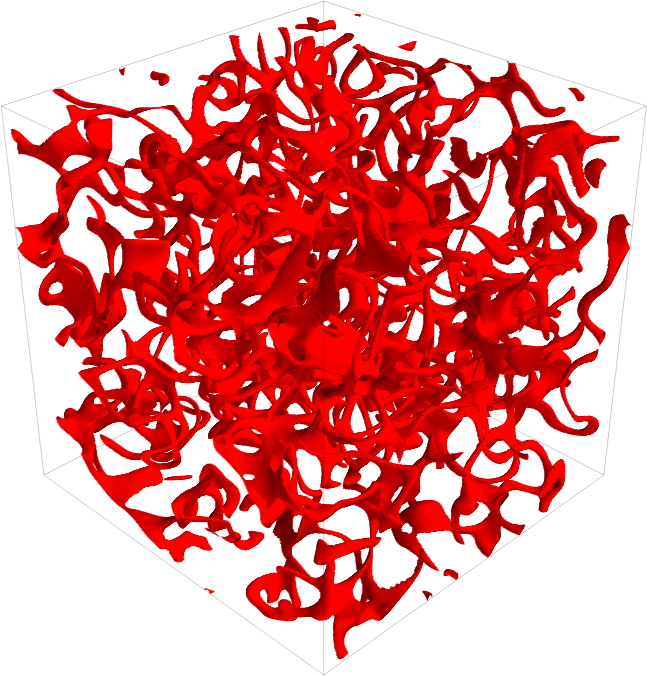
\includegraphics[width=0.25\linewidth]{nonequib/figures/IC/CF05-IC-t000}
    \raisebox{1.6in}{b)}~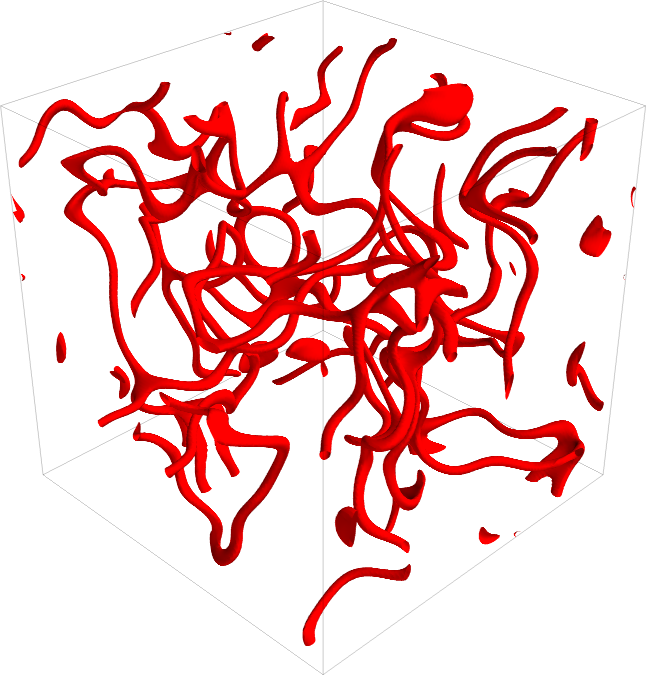
\includegraphics[width=0.25\linewidth]{nonequib/figures/IC/CF05-IC-t200}
    \raisebox{1.6in}{c)}~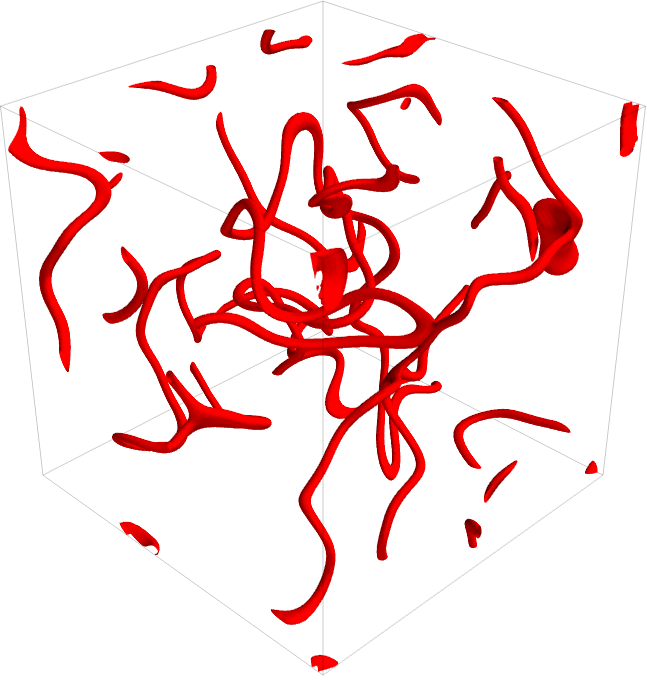
\includegraphics[width=0.25\linewidth]{nonequib/figures/IC/CF05-IC-t400}\\
    \raisebox{1.6in}{d)}~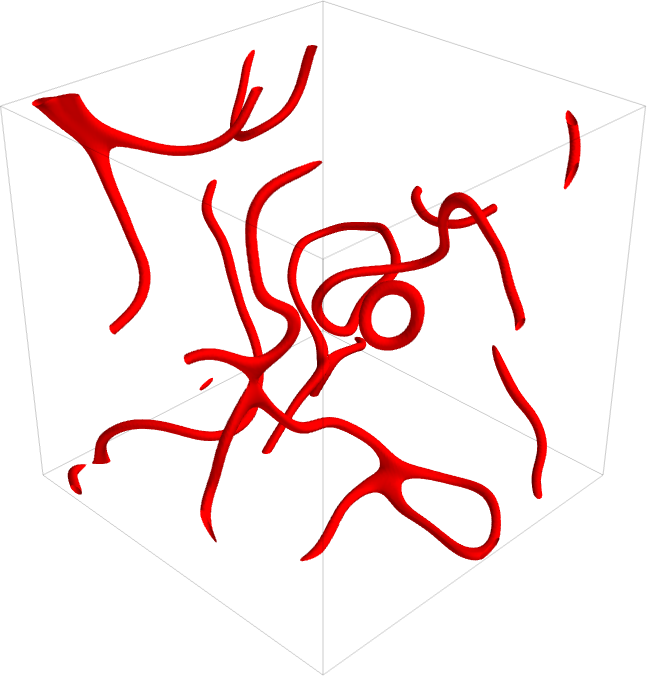
\includegraphics[width=0.25\linewidth]{nonequib/figures/IC/CF05-IC-t800}
    \raisebox{1.6in}{e)}~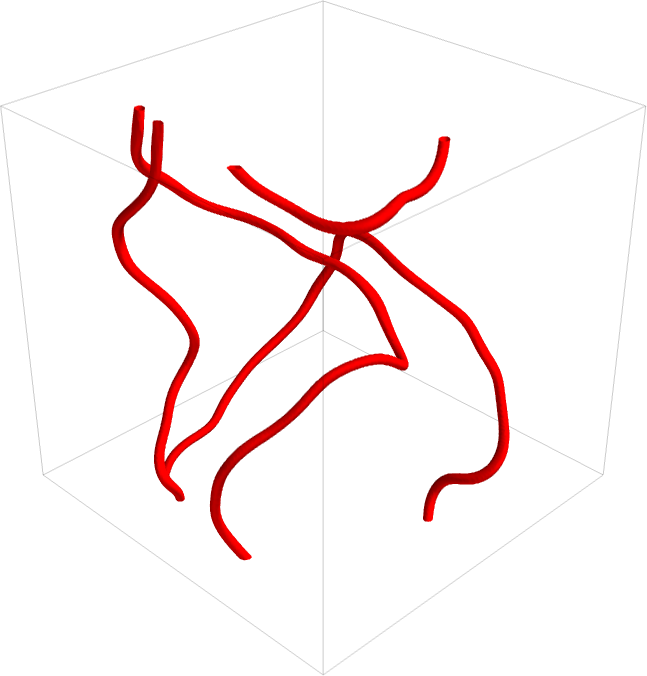
\includegraphics[width=0.25\linewidth]{nonequib/figures/IC/CF05-IC-t1600}
    \raisebox{1.6in}{f)}~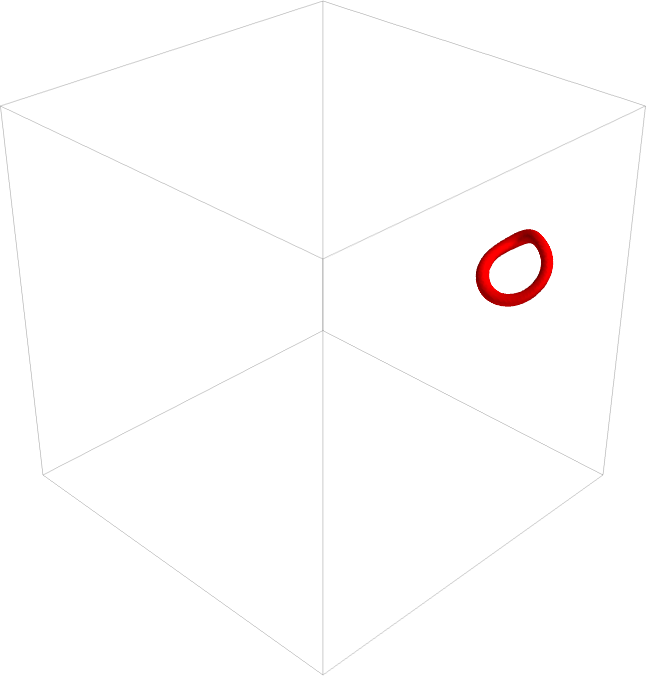
\includegraphics[width=0.25\linewidth]{nonequib/figures/IC/CF05-IC-t4000}
    \caption{A sample evolution of the turbulent vortex tangle present in the condensed part of the Bose gas as it decays to equilibrium. Here the condensate fraction of the gas is $\rho_0/\rho = 0.48$. Shown are iso-surfaces of the quasi-condensate density at isosurface level $0.05\braket{|\hat{\psi}|^2}$ at times (a) $t/\tau=0$, (b) $500$, (c) $1000$, (d) $2000$, (e) $4000$, and (f) $10\,000$. At later times (not shown) all vortex lines dissipate from the system.
}
    \label{fig:thermal}
\end{figure}

The raw wavefunction, $\psi$, is too noisy to allow direct visualisation of the resulting superfluid vortex tangle. This is overcome by defining a quasi-condensate wavefunction $\hat{\psi}$, as established in \cite{PhysRevA.66.013603}. High-frequency modes are filtered from the classical field wavefunction by transforming the complex amplitudes via $\hat{a}_{{\bf k}} = a_{{\bf k}}\times\max\{1-k^{2}/k_c^2,0\}$. This filtering technique is demonstracted in Section \ref{section:quasi-condensate} and is analogous to spatial course-grained averaging, so that $\hat{\psi}$ contains the long-wavelength component of the classical field only.  The condensate fraction, $\rho_0/\rho$, is defined as the proportion of the entire gas within the quasi-condensate. Note that while GPE dynamics conserves $N$ for the entire gas, the quasi-condensate particle number is free to vary. As occupation of the low-$k$ modes grows and the quasi-condensate forms, $\rho_0/\rho$ grows significantly, but stabilises near its equilibrium value before the vortex tangle decays significantly. 

Its physical properties, e.g. temperature and condensate fraction, are uniquely determined by $N$ and the kinetic energy of the system~\cite{PhysRevLett.95.263901}.  The equilibrium state of the non-condensed particles follows the Rayleigh-Jeans distribution, modified by the nonlinear interaction with the condensed particles \cite{PhysRevLett.95.263901}.  It is interesting to note that the equilibrium condensate fraction is insensitive to the number of modes, providing that the number of modes is, or exceeds, $16^3$ modes.  This suggests that this number of modes is sufficient to model the thermodynamic limit of the system. For comparison, we employ $192^3$ modes.

The quasi-condensate wavefunction is used to visualise the condensed part of the Bose gas, using evolving iso-surface levels of $|\hat{\psi}|^2 = 0.05\braket{|\hat{\psi}|^2}$. This level was chosen so that the resulting vortex structures are shown with approximately constant cross-sectional radius similar to the radius of a true vortex core (facilitated by the approximate quasi-condensate density term $\braket{|\hat{\psi}|^2}$).

\subsection{Approximate temperature of the gas}
\begin{figure}
\begin{center}
\begin{tikzpicture}
  \begin{axis}[samples=350,ylabel near ticks,xlabel near ticks,
      width=0.5\linewidth,
        xlabel=$T/T_\lambda$,
        ylabel=$\rho_0/\rho$,
        xmin=0,
        xmax=1.05,
        ymin=0,
        ymax=1.05,
        major tick length = 0.07cm]
    \addplot+[mark=none,color=black,thick] {1 - (1 - 0.2275*sqrt(0.5))*x - 0.2275*sqrt(0.5)*x^2};
    \addplot+[mark=none,color=black,dashed,thick] {(1 - x)^(2/3)};
  \end{axis}
\end{tikzpicture}%
\end{center}
\caption{\label{fig:cfvst}The condensate fraction and temperature relation for a weakly-interacting Bose gas for our simulation parameters (black solid line) and for an ideal non-interacting Bose gas (black dashed line).}
\end{figure} 

As we first saw in Section \ref{section:becinintro}, using the statistical mechanics of bosons it can be shown that for a {\it non-interacting} ideal gas of bosons there exists a simple prediction for how the condensate fraction of the gas grows as temperature decreases \cite{Pethick},
\begin{equation}
N_0 = N \left [ 1-\left ( \frac{T}{T_\lambda} \right )^\beta \right ],
\end{equation}
where $N_0$ is the number of condensed particles, $T_{\lambda}$ is the critical temperature for condensation and $\beta$ is a parameter that depends on the geometry of the system. For particles in a 3 dimensional box, $\beta=3/2$ \cite{Pethick}. By inverting this relation we could obtain a simple minded approximation for the temperature of our equilibrated Bose gas, ignoring interactions.

However, Youd {\it et al.} \cite{berloff_2007} recently provided the following empirical relationship for a {\it weakly-interacting} Bose gas in a 3 dimensional box:
\begin{equation}
  \frac{T}{T_\lambda} = 1 - (1 - \alpha\sqrt{\rho})\frac{\rho_0}{\rho} - \alpha\sqrt{\rho}\,\left(\frac{\rho_0}{\rho}\right)^2,
  \label{eq:temp}
\end{equation}
where $\alpha=0.2275$ is a fitting parameter. We will use this relation throughout the chapter to evaluate the temperature of the gas using the condensate fraction at equilibrium. The relation is compared to the relation for an ideal non-interacting Bose gas in Figure \ref{fig:cfvst}. Table \ref{tbl:cond_frac} lists the resulting approximate temperatures at equilibrium for the parameters chosen in our simulations.

\subsection{Energy scales of the vortex tangle}


\begin{figure}
\centering
\begin{tikzpicture}
    \begin{axis}[ylabel near ticks,xlabel near ticks,
        width=0.6\linewidth,
        xlabel={},
        ylabel={},
        xmin=0.025,
        xmax=9,
        ymin=5e-5,
        ymax=10,
        major tick length = 0.00cm,
        minor tick length = 0.00cm,
    xmode=log,
    ymode=log,
    axis y line*=right,
        axis x line*=top,
        ytick={0},
        yticklabels={,,},
        xtick={0.043,0.1709,6.28},
        xticklabels={$k_D$, $k_\ell$, $k_\xi$} ]  
          \addplot+[mark=none,black!99,ultra thick,dashed,domain=1.3:3.45] {(3e-2)*x^(-3)};
      \addplot+[mark=none,black!99,ultra thick,dashed,domain=0.1:0.5] {(6e-1)*x^(-1)};    
          \addplot+[mark=none,black!50,dashed] coordinates {(6.28, 1e-5) (6.28, 10)};
      \addplot+[mark=none,black!50,dashed] coordinates {(0.043, 1e-5) (0.043, 10)};
      \addplot+[mark=none,black!50,dashed] coordinates {(0.1709, 1e-5) (0.1709, 10)};
    \end{axis}
    \begin{axis}[samples=200,ylabel near ticks,xlabel near ticks,
        width=0.6\linewidth,
        xtick pos=left,
        ytick pos=left,
        xlabel=$k \xi$,
        ylabel=$\hat{E}^i_{\rm kin}/\mu$,
        xmin=0.025,
        xmax=9,
        ymin=5e-5,
        ymax=10,
        axis y line*=left,
        axis x line*=bottom,
        major tick length = 0.1cm,
        minor tick length = 0.07cm,
    xmode=log,
    ymode=log,
    restrict expr to domain={x}{0.0001:4.5}]
      \addplot+[red,only marks,mark options={scale=0.5}] file {nonequib/kk_vs_Eikin-CF02-t300.dat};
      \addplot+[green,only marks,mark options={scale=0.5}] file {nonequib/kk_vs_Eikin-CF05-t300.dat};
      \addplot+[mark=diamond*,blue,only marks,mark options={scale=0.7}] file {nonequib/kk_vs_Eikin-CF075-t300.dat};
      \node at (axis cs: 3,0.004) {$k^{-3}$};
      \node at (axis cs: 0.25,5.5) {$k^{-1}$};
    \end{axis}
  \end{tikzpicture}
  \caption{\label{fig:spectra}Incompressible kinetic energy spectrum for the quasi-condensate tangles with $\rho_0/\rho=0.22$ (red circles), $\rho_0/\rho=0.48$ (green squares), and $\rho_0/\rho=0.77$ (blue diamonds) at time $t/\tau=300$. Dashed lines show the length scale of the healing length, $k_\xi$, the length scale of inter-vortex spacing $k_\ell$, the length scale of the periodic box $k_D$. Guide lines proportional to $k^{-3}$ and $k^{-1}$ are also shown. }
\end{figure}
One method to characterise the turbulence of the vortex tangle formed in the quasi-condensate is by studying how the kinetic energy of the vortices is distributed over length scales. There are three length scales of particular interest, $k_D=2\pi/D$ is the length scale associated with the computational box, $k_\xi = 2\pi/\xi$ is the length scale associated with the superfluid healing length, and $k_\ell$ is the length scale associated with the inter-vortex spacing, $\ell$. The inter-vortex spacing can be approximated by $1/\sqrt{L}$, a relation derived through dimensional arguments where $L$ is the vortex line-density (length of vortex line per unit volume). These length scales provide the perspective required to interpret the distribution of energy.

The kinetic energy of the quasi-condensate is defined as $E_{\rm kin} = \frac{\hbar^2}{2m}|\nabla \hat\psi|^2$.
 Using Parseval's theorem, the corresponding kinetic energy spectrum, $\hat{E}_{\rm kin}(k)$, can be written in terms of the angle-average of $\left |\mathcal{F}(\sqrt{E_{\rm kin}})\right |^2$ \cite{Nore},
where $\mathcal{F}$ denotes the Fourier transform, so that,
\begin{equation}
  \int E_{\rm kin}({\bf r})~{\rm d}^3{\bf r} = \int \hat{E}_{\rm kin}(k)~{\mathrm d}k.
  \label{eq:Ekin}
\end{equation}
The kinetic energy can be further decomposed into compressible and incompressible parts, $E_{\rm kin} = E^i_{\rm kin} + E^c_{\rm kin}$, by using the decomposition $\sqrt{n}v_j = (\sqrt{n}v_j)^c + (\sqrt{n}v_j)^i$, with $\nabla(\sqrt{n}v_j)^i=0$, where $n$ is the fluid density and $\mathbf{v}$ is the fluid velocity. The incompressible kinetic energy spectrum is then denoted $\hat{E}^i_{\rm kin}(k)$, defined similarly to $\hat{E}_{\rm kin}(k)$.

We calculate the incompressible energy spectrum of the quasi-condensate at various temperatures, sampled at time $t/\tau=300$ so as to characterise the vortex tangle before significant decay, while providing enough time for the quasi-condensate to form. The resulting spectra are shown in Figure \ref{fig:spectra}. The majority of each spectrum demonstrates a $\sim k^{-3}$ scaling, corresponding to the vortex core on the scale of $k_\ell<k<k_\xi$. For quasi-classical turbulence, we would expect a build up of kinetic energy at scales larger than the inter-vortex distance, $k_D<k<k_\ell$, demonstrating the famous Kolmogorov $k^{-5/3}$ power law scaling. In our simulations the incompressible kinetic energy spectrum does {\it not} show a definitive $k^{-5/3}$ scaling. The spectra instead show a marked lack of energy build up at scales $k_D<k<k_\ell$. In contrast to quasi-classical turbulence, ultra-quantum turbulence predicts a $k^{-1}$ scaling at scales $k_D<k<k_\ell$. A guide line proportional to this power law is shown Figure \ref{fig:spectra}.

\section{Relaxation of the vortex tangle}
As the condensate evolves over the course of the simulation, the initially-formed dense vortex tangle remains random and isotropic throughout the decay to one or more vortex rings, which eventually also decay, leading to a vortex-free state (the ``equilibrated" state). A example of such a decay is shown in Figure \ref{fig:thermal}.

Insight into the nature of the quasi-condensate turbulence can be obtained by investigating the relaxation of the vortex tangle, obtained by monitoring the vortex line-density $L$. We estimate the vortex line-length from the total volume of the isosurface tubes, $V_{\rm t}$. We assume that each vortex tube has uniform constant circular cross-sectional area $A_{\rm t}$; the total vortex line-length is then $V_{\rm t}/A_{\rm t}$. Note that this approximation is only strictly valid for vortices well separated in space and for steady condensate fraction (so that the healing length of the quasi-condensate is constant). We nevertheless find that the estimate is accurate enough for our analysis.

\begin{figure}
\centering
\begin{tikzpicture}
  \begin{axis}[samples=200,ylabel near ticks,xlabel near ticks,
      width=0.45\linewidth,
      xtick pos=left,
      ytick pos=left,
      xlabel=$t/\tau$,
      ylabel=$L\xi^2$,
      xmin=10,
      xmax=15000,
      ymin=1.5e-5,
      ymax=3e-3,
      major tick length = 0.1cm,
      minor tick length = 0.07cm,
      xmode=log,
      ymode=log]
      \addplot+[mark=diamond*,blue,only marks,mark options={fill=blue}] table[x=t,y=l] {nonequib/l_vs_t_CF075.dat};
      \addplot+[green,only marks,mark=square*,mark options={fill=green,scale=0.7}] table[x=t,y=l] {nonequib/l_vs_t_CF05.dat};
      \addplot+[red,only marks,mark=*,mark options={fill=red,scale=0.7}] table[x=t,y=l] {nonequib/l_vs_t_CF02.dat};
      \addplot+[mark=none,black,ultra thick,dashed,domain=600:3000] {(6e-1)*x^(-1)};
      \node at (axis cs: 2000,6e-4) {$t^{-1}$};
  \end{axis}
\end{tikzpicture}
\begin{tikzpicture}
    \begin{axis}[samples=200,ylabel near ticks,xlabel near ticks,
      width=0.45\linewidth,
      ylabel near ticks,
      xlabel near ticks,
      xtick pos=left,
      ytick pos=left,
      ylabel={$\rho_0/\rho$},
      xlabel={$t/\tau$},
      xmin=0,
      xmax=5000,
      ymin=0,
      ymax=1.1]
      \addplot+[red,mark=none,ultra thick] file {nonequib/cf_vs_t_CF02.dat};
      \addplot+[green,mark=none,ultra thick,dashed] file {nonequib/cf_vs_t_CF05.dat};
      \addplot+[blue,mark=none,ultra thick,dash pattern=on 4pt off 1pt on 1pt off 1pt] file {nonequib/cf_vs_t_CF075.dat};
    \end{axis}
\end{tikzpicture}
\caption{\label{fig:ll_t} Vortex line density over time for $\rho/\rho_0=0.22$ (red circles), $\rho/\rho_0=0.48$ (green sqaures), and $\rho/\rho_0=0.77$ (blue diamonds). Each line is an average of 5 simulations. A line proportional to $t^{-1}$, characteristic of the decay of a ultra-quantum turbulence, is shown (dashed black line) as reference. (Inset) Condensate fraction over time for equilibrium states for $\rho/\rho_0=0.22$ (red solid line), $\rho/\rho_0=0.48$ (green dashed line), and $\rho/\rho_0=0.77$ (blue dot-dashed line). }
\end{figure}

\begin{table}
\centering
\begin{tabular}{ccc}
{\it $\rho_0/\rho$} & {\it Power law fit} & {\it $95\%$ confidence interval} \\
\hline \\ [-2ex]
$0.22$ & $-1.04$ & $(-1.10, -0.98)$\\
$0.48$ & $-0.95$ & $(-1.01, -0.89)$\\
$0.77$ & $-0.81$ & $(-0.89, -0.72)$\\
\hline
\end{tabular}
\caption{The resulting value of $b$ for fitting the decay of the vortex line density over time to the equation $f(t) = at^b+c$ for the data demonstrated in Figure \ref{fig:ll_t}, including a $95\%$ confidence interval.}
\label{tbl:fits}
\end{table}

The decay of the vortex line density is shown in Figure \ref{fig:ll_t}. When the condensate fraction at the simulated value of $\rho_0/\rho = 0.22$, the decay of $L$ is in good agreement with the predicted ultra-quantum decay of $L(t) \propto t^{-1}$. Our cooler simulations show a deviation from the $t^{-1}$ decay law, suggesting a shift to longer vortex tangle decay times as the gas is simulated closer to the zero temperature limit. The decays are quantitatively compared to the predicted power law in Table \ref{tbl:fits}, showing a power law best fit and $95\%$ confidence interval.

The velocity correlation function, $f(r)$, is defined at a fixed point in time as
\begin{equation}
f(r) = \frac{\langle v_x({\bf r})v_x({\bf r} +  r\hat{\bf e}_x) \rangle}{\langle v_x({\bf r})^2 \rangle}
\end{equation}
where $\mathbf{v}$ is the quasi-condensate fluid velocity and the ensemble average is performed over positions ${\bf r}$. The function is a dimensionless measure of velocity correlation at distance $r$, with $f(0)=1$, and is shown in Figure \ref{fig:IS_t} (a) for the three of our simulated parameter sets (spanning the range of temperatures) at a time of $t/\tau = 300$. The choice of time allows us to probe the velocity correlations after the quasi-condensate has formed, but before any significant decay of the vortex tangle has taken place. For the time chosen, the velocity correlation functions are not significantly different for each of our simulation parameters. The value of $f(r)$ smoothly drops to approximately at around $r/\xi = 20$. Short scale correlation is expected due to the structure of the fluid velocity around a vortex core. The lack of velocity correlation at large scales suggests a lack of vortex bundles (collections of co-rotating aligned vortex lines of the same circulation), theorised to be the driving force of the large scale kinetic energy in quasi-classical turbulence.

The integral scale provides a convenient measure of the distance over which velocities are correlated by producing a scalar value from the velocity correlation function. It is defined as
\begin{equation}
I = \int\limits_0^\infty\! f(r)\, \mathrm{d}r,
\end{equation}
and is shown in Figure \ref{fig:IS_t} (b) evolving over time during the vortex tangle evolution. Three lines corresponding to different temperatures are shown, with each line an average of 5 simulations. The value of $I$ increases as the vortex tangle decays in all of the simulated cases, an expected result as vortices decay and so velocity becomes correlated over larger regions of space. At early times, $I(0)\approx0$, reflecting the random nature of the initial tangle. As the tangle decays, the value of $I$ grows, but remains significantly less than $\ell$, demonstrating that as the vortex tangle evolves over time, there is no evidence of vortex lines ``bundling up'' to create a large scale flow.

\begin{figure}
\centering
\begin{tikzpicture}
  \begin{axis}[samples=200,ylabel near ticks,xlabel near ticks,
        width=0.45\linewidth,
        xtick pos=left,
        ytick pos=left,
        xlabel={\footnotesize $r/\xi$},
        ylabel={\footnotesize $f$},
        xmin=0,
        xmax=20,
        ymin=-0.1,
        ymax=1.1,
        major tick length = 0.1cm,
        minor tick length = 0.07cm]
      \addplot+[red,mark=none,ultra thick] file {nonequib/f_vs_r_CF02.dat};
      \addplot+[green,mark=none,ultra thick,dashed] file {nonequib/f_vs_r_CF05.dat};
      \addplot+[blue,mark=none,ultra thick,dash pattern=on 4pt off 1pt on 1pt off 1pt] file {nonequib/f_vs_r_CF075.dat};
    \end{axis}
  \end{tikzpicture}
\begin{tikzpicture}
    \begin{axis}[samples=200,ylabel near ticks,xlabel near ticks,
    width=0.45\linewidth,
    ylabel near ticks,
    xlabel near ticks,
    xtick pos=left,
        ytick pos=left,
        ylabel={$I/\xi$},
        xlabel={$t/\tau$},
        xmin=0,
        xmax=5000,
        ymin=0,
        ymax=65]
      \addplot+[green,mark=square*,thick,mark options={fill=green,scale=0.7}] file {nonequib/IS_vs_t_CF05.dat};
      \addplot+[red,mark=*,thick,mark options={fill=red}] file {nonequib/IS_vs_t_CF02.dat};
      \addplot+[blue,mark=diamond*,thick,mark options={fill=blue}] file {nonequib/IS_vs_t_CF075.dat};
      %\addplot+[black,thick,mark=none,dashed] table[x expr=\thisrow{t}, y expr=1/sqrt(\thisrow{l})] {l_vs_t_CF075.dat};
    \end{axis}
  \end{tikzpicture}
  \caption{\label{fig:IS_t}(Color online) The integral scale as the quasi-condensate vortex tangle decays, for $\rho/\rho_0=0.22$ (red circles), $\rho/\rho_0=0.48$ (green sqaures), and $\rho/\rho_0=0.77$ (blue diamonds). Also shown is the estimated inter-vortex distance $\ell = 1/\sqrt{L}$ for the case with $\rho/\rho_0=0.77$ (dashed line). (Inset) A snapshot of the velocity correlation function $f(r)$ at time $t = 300\tau$ for equilibrium states for $\rho/\rho_0=0.22$ (red solid line), $\rho/\rho_0=0.48$ (green dashed line), and $\rho/\rho_0=0.77$ (blue dot-dashed line).}
\end{figure}

The results of the velocity correlation and integral scale measurements confirm the conclusions of the kinetic energy spectrum measurements, there is no evidence of energy at scales larger than the inter-vortex spacing at any point during vortex decay, at all simulated temperatures. This is perhaps not such a surprising result, the initial vortex tangle is seeded and forms from random fluctuations in the phase of the 3D wavefunction, favouring the random nature of quasi-classical turbulence.


\section{Moving obstacle at finite-temperature\label{sec:obstacle}}
\subsection{Critical velocity for vortex nucleation}
Having obtained the equilibrated finite-temperature states of the Bose gas, we now move on to consider a laser-induced obstacle moving through the gas.  The obstacle, uniform in $z$, is translated in the $x$-direction at speed $v$.  Our simulations are conducted moving with the obstacle, transformed into the moving frame as in Section \ref{section:linearmovframe}. The obstacle is imposed through a time-independent cylindrical Gaussian potential, as described in Section \ref{section:3dcylinderpotential},
\begin{equation*}
  V({\bf r}) = V_0 \exp\left ( -\frac{x^2+y^2}{d^2}\right ),
\end{equation*}
where $d$ and $V_0$ parametrise the width and amplitude of the potential. The amplitude is linearly increased from $V_0 = 0$ at first introduction to its maximal value $V_0=5\mu$ over a period of $200\tau$.   The frame speed is increased adiabatically to the required value according to the temporal profile $v \tanh(\hat{t}/200 \tau)$, where $\hat{t}$ denotes the time from introduction of the obstacle.

Simulations are repeated (from identical initial conditions) with increasing terminal speeds (in steps of $0.057c$) until vortices are detected.  Vortex detection is by visual inspection of the filtered density, up to a maximum simulation time $\hat{t}=500\tau$ (which is long enough to ensure that the obstacle is fully introduced and at terminal speed, but otherwise arbitrary). This procedure defines the critical velocity $v_c$.  There is a systematic uncertainty in our measurement of $v_c$, arising from the discrete terminal speeds employed.  Note that we have repeated this process for multiple randomized initial conditions, and find no change in our measurement of $v_c$; that is, the systematic uncertainty due to using discretised speeds is larger than the statistical uncertainty arising from different random initial conditions.

\begin{figure}
\hspace*{1cm}(a)\hspace{7cm}(b)\hspace{3cm}
\begin{center}
  \begin{tikzpicture}
  \begin{axis}[samples=200,ylabel near ticks,xlabel near ticks,
        width=0.45\linewidth,
        xtick pos=left,
        ytick pos=left,
        xlabel=$\rho_0/\rho$,
        ylabel=$v_c/c$,
        xmin=0,
        xmax=1.1,
        ymin=0,
        ymax=0.55,
        major tick length = 0.07cm
      ]
      \addplot+[only marks,mark options={blue},error bars/error bar style={blue},  error bars/.cd,y dir=both,y explicit] table[x=cf,y=2xi,y error=2err] {nonequib/cf_vs_vc.dat};
      \addplot+[only marks,mark=square*,mark options={red},error bars/error bar style={red},  error bars/.cd,y dir=both,y explicit] table[x=cf,y=5xi,y error=5err] {nonequib/cf_vs_vc.dat};
      \addplot+[mark=none,color=black!50,thick,dashed] [domain=0:1.5] {0.46*sqrt(x)};
      \addplot+[mark=none,color=black!50,thick,dashed] [domain=0:1.5] {0.35*sqrt(x)};
    \end{axis}
    \begin{axis}[ylabel near ticks,xlabel near ticks,
        width=0.45\linewidth,
        xlabel=$T/T_\lambda$,
        ylabel={},
        xmin=0,
        xmax=1.1,
        ymin=0,
        ymax=1,
        major tick length = 0.07cm,
        axis y line*=right,
        axis x line*=top,
        yticklabels={,,},
        ytick={0},
        xtick={0,0.23,0.44,0.64,0.82,1},
        xticklabels={$1$, $0.8$, $0.6$, $0.4$, $0.2$,$0$}
        ]
    \end{axis}
  \end{tikzpicture}%
  \begin{tikzpicture}%
  \begin{axis}[samples=200,ylabel near ticks,xlabel near ticks,
        width=0.45\linewidth,
        xtick pos=left,
        ytick pos=left,
        xlabel=$d/\xi$,
        ylabel=$v_c/c$,
        xmin=0,
        xmax=23,
        ymin=0.17,
        ymax=0.35,
        major tick length = 0.07cm
      ]
      \addplot+[only marks,mark options={blue},error bars/error bar style={blue},  error bars/.cd,y dir=both,y explicit] table[x=d,y=vc,y error=err] {nonequib/d_vs_vc.dat};
      \addplot+[mark=none,color=black!50,thick,dashed] [domain=0:30] {0.26/x+0.18};
    \end{axis}
  \end{tikzpicture}
\end{center}
  \caption{\label{fig:vc-n0}(a) Critical velocity $v_{\rm c}$ for the moving Gaussian-shaped obstacle (uniform in $z$) as a function of condensate fraction $\rho_0/\rho$ and temperature $T/T_\lambda$, for obstacle widths $d=2\xi$ (blue circles) and $d=5\xi$ (red squares). The dotted lines show the analytic model $v_{\rm c}=\beta \sqrt{\rho_0/\rho}$ with fitted coefficients $\beta=0.46c$ and $0.35c$. (b) The critical velocity approaches an asymptotic value as the obstacle size is increased. Included is a fit of the form $v_{\rm c}=\alpha/d+\gamma$ with $\alpha=0.26~(\xi^2/\tau)$ and $\gamma=0.18 c$.  Errors bars represent the systematic uncertainty in $v_c$ due to the discretised values of $v$ considered.}
\end{figure}

Figure \ref{fig:vc-n0} (a) shows the variation of $v_c$ with both condensate fraction $\rho_0/\rho$ (lower abscissa) and temperature $T/T_\lambda$ (upper abscissa), for two example obstacles widths.  The critical velocity has a maximum value at zero temperature (unit condensate fraction), and decreases nonlinearly as temperature increases (condensate fraction decreases), reaching zero at the critical point for condensation.

At zero temperature, the critical velocity is of the order of the condensate speed of sound $c=\sqrt{\rho g/m}$, with a general form $v_{\rm c}(T=0)=\beta c$,
where $\beta$ is a parameter which depends solely on the shape of the
obstacle (here $d$ and $V_0$).  The simulated $v_c$ data in
Figure \ref{fig:vc-n0} closely follow the simple functional form
$v_{\rm c}(T) = v_{\rm c}(0) \sqrt{\rho_0/\rho}$, as shown by the dashed lines.
An expression for the critical velocity valid at zero and non-zero
temperatures is
\begin{equation}
v_{\rm c}(T)=\beta \sqrt{\rho_0 g/m}.
\label{eqn:finite_vc}
\end{equation}
In other words, for a given obstacle, the critical velocity is a fixed
fraction of the speed of sound based on the {\it condensate} density
rather than the total particle density \cite{leadbeater_2003}.

Figure \ref{fig:vc-n0} (b) shows the variation of $v_{\rm c}$ with the obstacle width $d$ at finite temperature, for the example of $T/T_\lambda =0.56$.   The qualitative behaviour is consistent with that seen in Chapter \ref{cha:wake} at zero temperature \cite{huepe00,rica2001,stagg_parker_14}: for small $d$ the critical velocity is sensitive to $d$ (due to the prominence of boundary layer effects) but as $d$ increases $v_c$ decreases towards a limiting values (the Eulerian limit).  However, the critical velocities are systematically reduced compared to the zero temperature case due to the reduced condensate speed of sound at finite temperature.


\subsection{Vortex nucleation pattern}
Finally we examine the manner in which vortices are nucleated from the obstacle.  At zero temperature, one expects the nucleation of straight anti-parallel vortex lines from the obstacle, either released in unison or staggered in time \cite{frisch92,saito10,stagg_parker_14}, which move downstream relative to the obstacle.  At finite temperature, we observe the loss of vortex symmetry along the obstacle axis, and three general regimes of vortex nucleation, with representative examples shown in Figure  \ref{fig:vort-lines}:

\begin{figure}
    %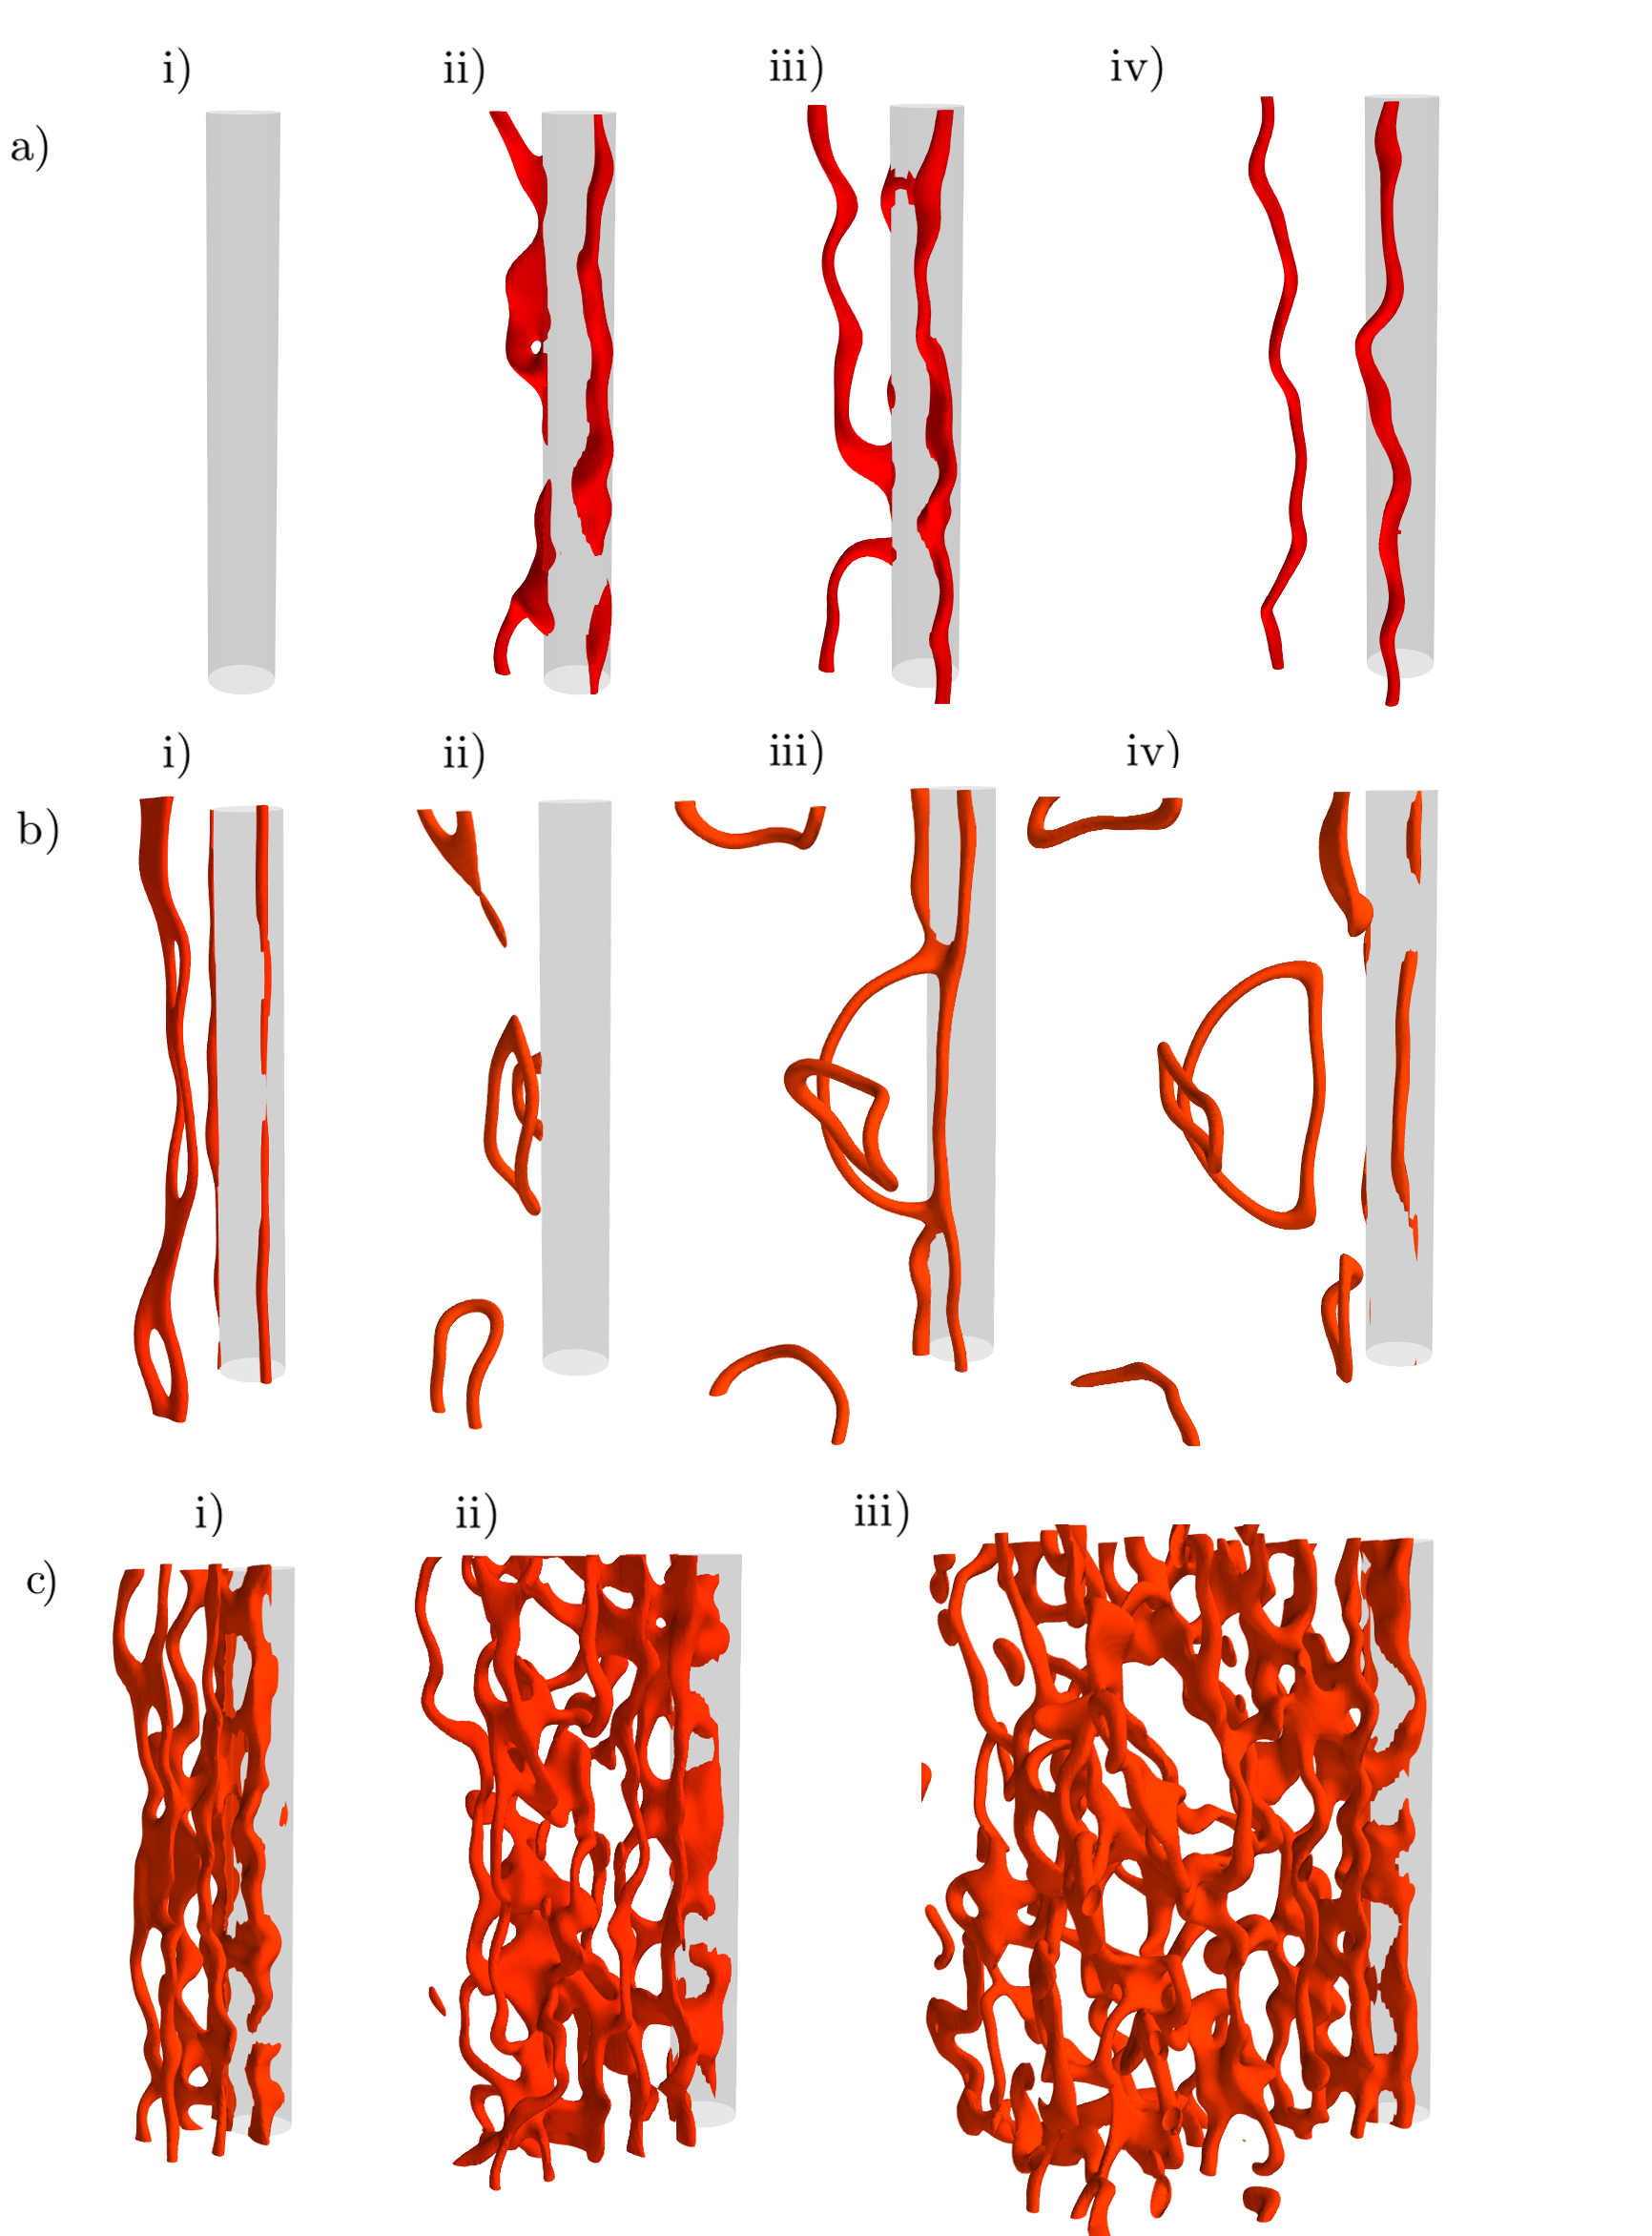
\includegraphics[width=0.9\linewidth]{nonequib/figures/vort}
    \centering
    \begin{tikzpicture}
      \node[anchor=south west] at (0,0) (image1) {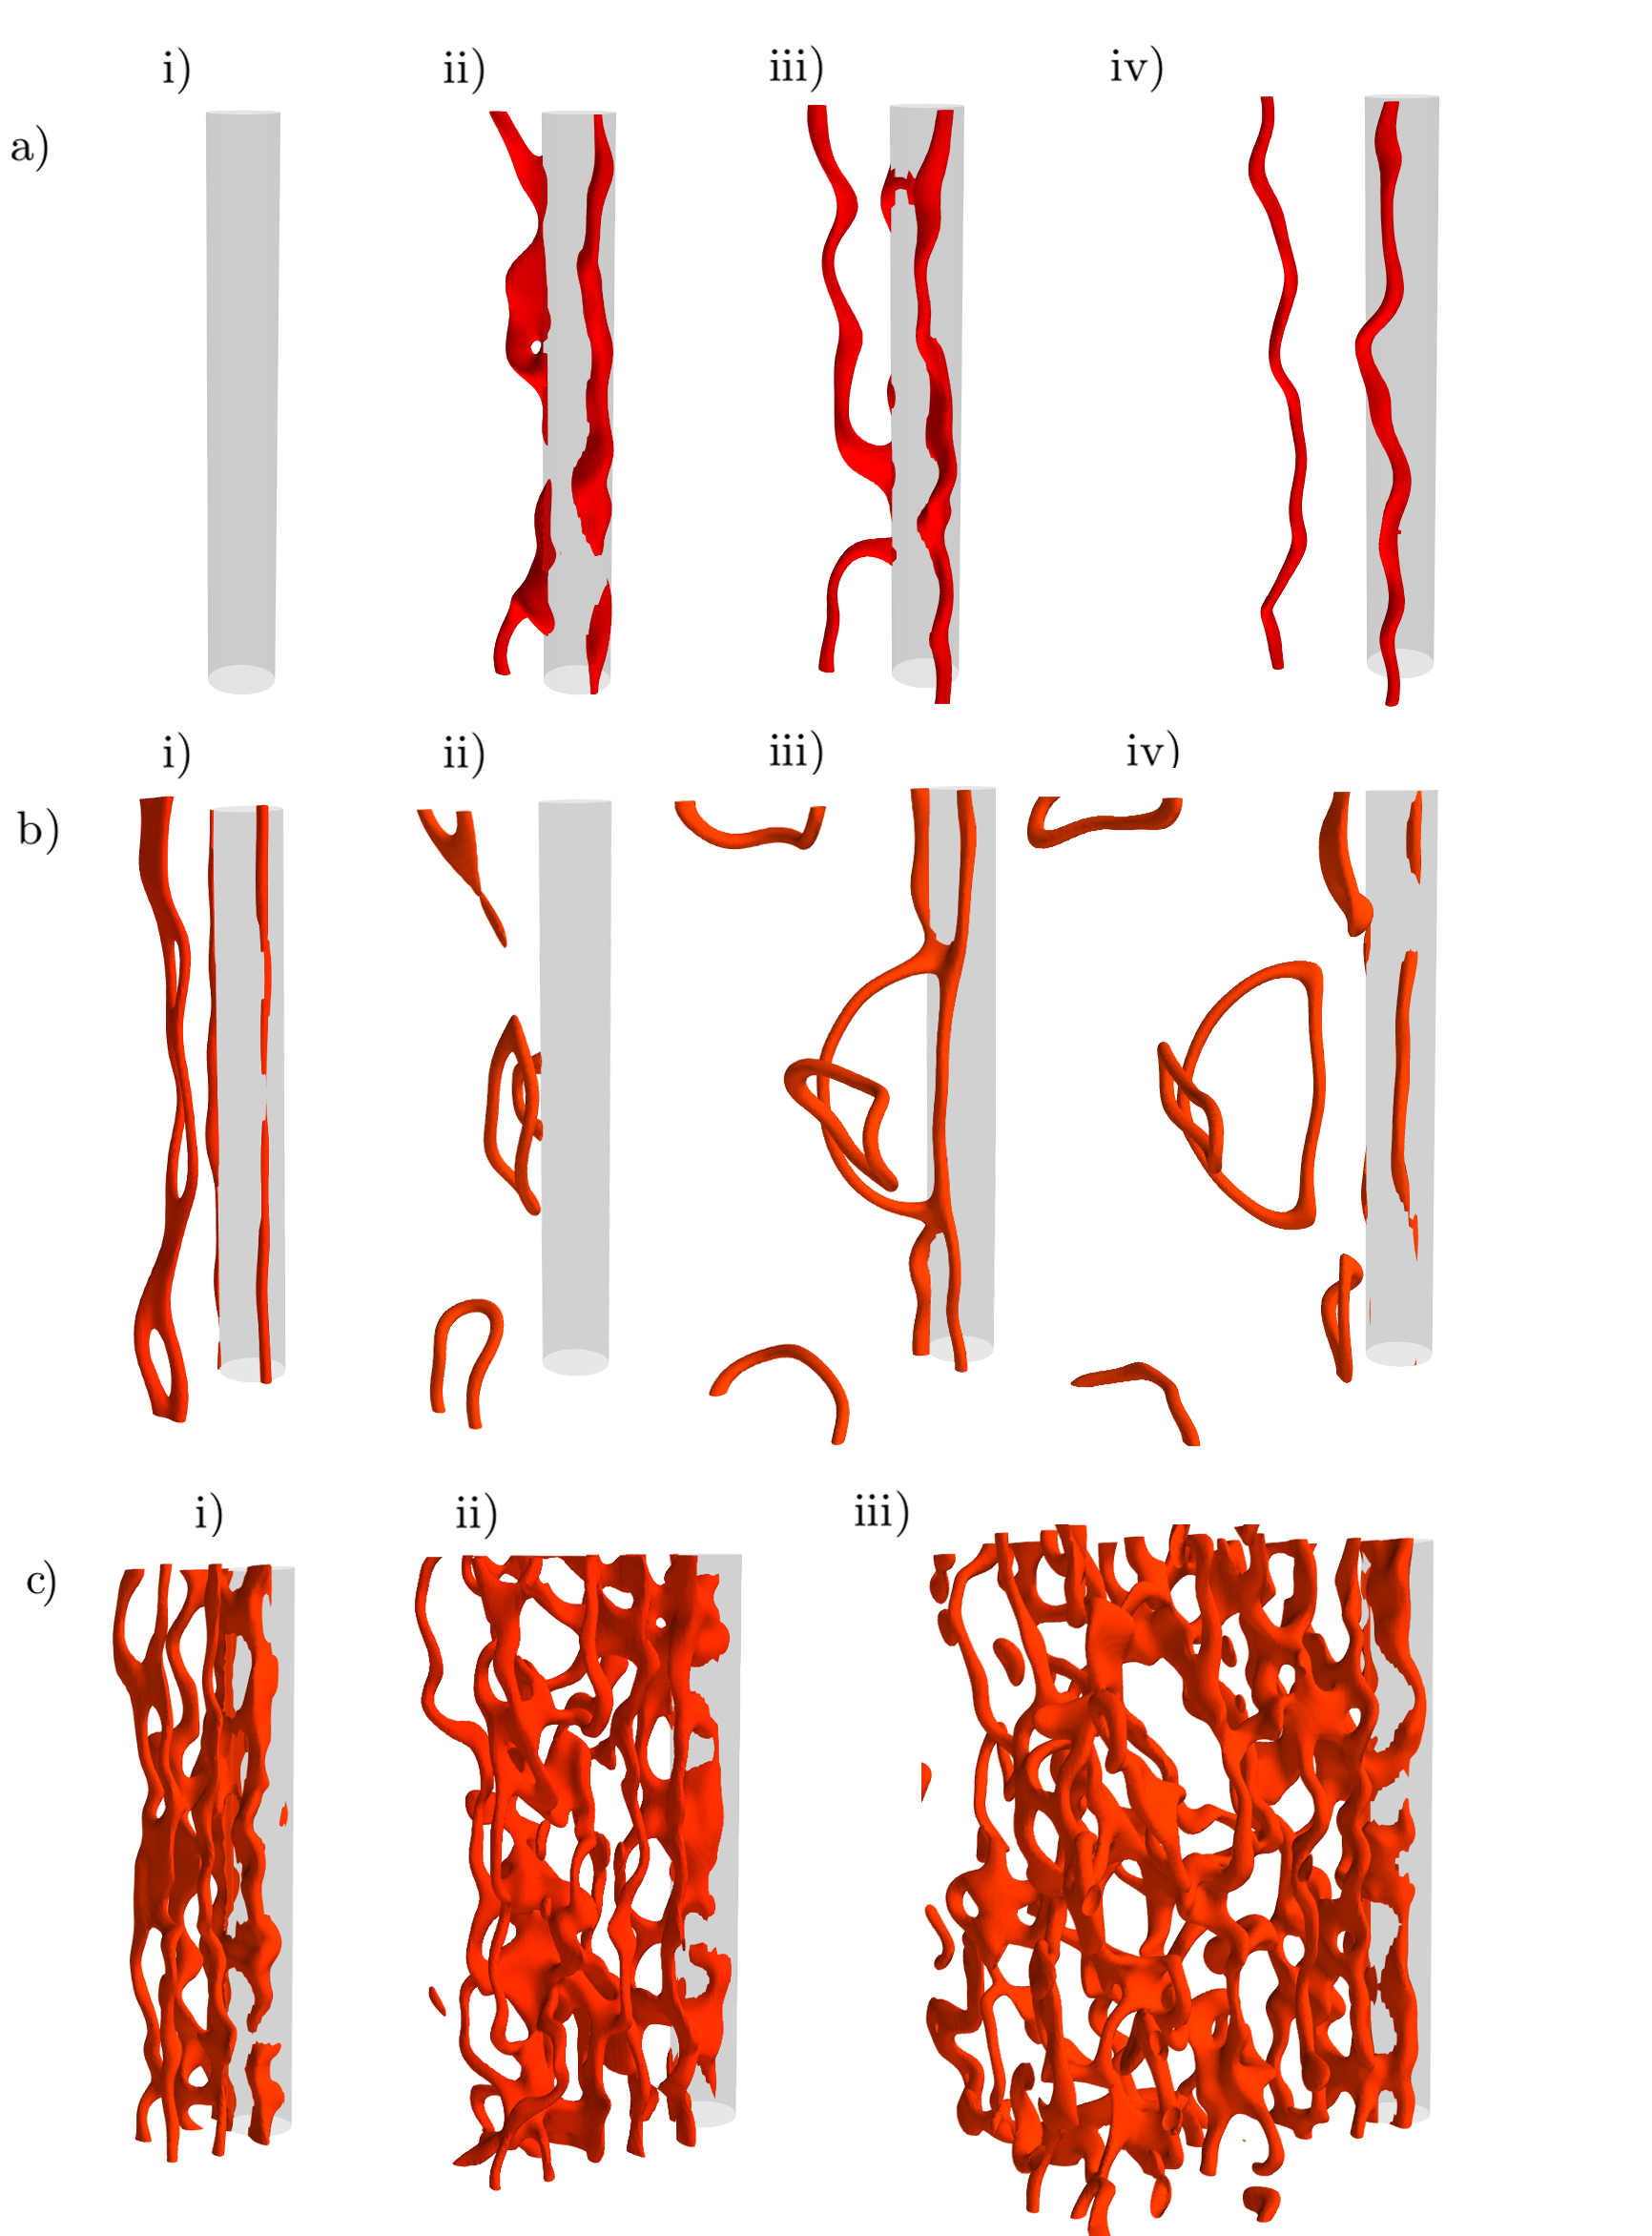
\includegraphics[width=0.9\linewidth]{nonequib/figures/vort}};
      \begin{scope}[x={(image1.south east)},y={(image1.north west)}]
      \node at (0.1,0.96) {i)};
      \node at (0.27,0.96) {ii)};
      \node at (0.46,0.96) {iii)};
      \node at (0.65,0.96) {iv)};

      \node at (0.1,0.66) {i)};
      \node at (0.27,0.66) {ii)};
      \node at (0.46,0.66) {iii)};
      \node at (0.65,0.66) {iv)};

      \node at (0.1,0.33) {i)};
      \node at (0.27,0.33) {ii)};
      \node at (0.56,0.33) {iii)};

      \node at (0.05,0.93) {a)};
      \node at (0.05,0.63) {b)};
      \node at (0.05,0.3) {c)};
      \end{scope}
    \end{tikzpicture}
    \caption{\label{fig:vort-lines} Snapshots of the typical vortex nucleation from the moving Gaussian-shaped obstacle with $d=5\xi$ (gray) in the finite temperature Bose gas. The three cases (a-c) are representative of the behaviour across the whole parameter space. Shown are  isosurfaces of the quasi-condensate density ($|\hat{\psi}|^2 = 0.05\braket{|\hat{\psi}|^2}$).  (a) Vortices are shed as pairs of anti-parallel vortex lines.  Here the system parameters are $\rho_0/\rho = 0.22$ and $v=0.17c$, and the snapshots correspond to times (i) $\hat{t}/\tau=210$, (ii) $460$, (iii) $585$ and (iv) $710$.  (b) Vortex rings are nucleated from the obstacle.  The system parameters are $\rho_0/\rho = 0.91$ and $v=0.42c$, and the times are (i) $\hat{t}/\tau=500$, (ii) $700$, (iii) $875$ and (iv) $950$. (c) A vortex tangle forms behind the obstacle. The system parameters are $\rho_0/\rho = 0.35$ and $v=0.59c$, and the times are (i) $\hat{t}/\tau=250$, (ii) $375$ and (iii) $500$. }
\end{figure}


\begin{description}
\item[Vortex lines] A pair of ``wiggly'' vortex lines is produced  [Figure  \ref{fig:vort-lines}(a)].  The wiggles are driven by the thermal fluctuations, which cause the vortex elements to be nucleated at slightly different times along the obstacle; this is visible at intermediate times (snapshots (iii) and (iv)).   These elements ultimately merge together along the axis of the obstacle to form a wiggly vortex/anti-vortex line. Similar vortex configurations
in the form of lines which are partially attached to a thin wire 
were also observed in liquid helium \cite{zieve2001}. 
\item[Vortex rings]  Here vortices predominately form vortex
rings [Figure \ref{fig:vort-lines}(b)].  The vortex loops generated
at the obstacle rapidly peel away from the obstacle, reconnecting with
adjacent loops to form rings. Due to the way the vortex rings form initially along the obstacle, they are elliptical and polarised such that they are longer along the obstacle axis. 
\item[Vortex tangle]  Strong
interaction between successively nucleated vortices leads to the formation of a complex tangle of vortex lines behind the obstacle [Figure \ref{fig:vort-lines}(c)].
\end{description}

While the vortex line regime is analogous to the zero temperature case, no analogue occurs for the ring and tangle regimes.   We note that even a small amount of thermal fluctuations is enough to vastly change the form of vortex nucleation, such as the vortex rings produced in Figure \ref{fig:vort-lines}(c) for a condensate fraction of $0.91$.

To systematically map the occurrence of these regimes, we measure the vortex line-density $L$ and vortex polarity $R$ (described below) at a fixed observation time of $\hat{t}=500\tau$, throughout the parameter space of flow velocity and condensate fraction.  The results are presented in Figure \ref{fig:vort-vals}.  Below the critical velocity (solid black line) no vortices are produced, and thus $L=0$.  Above the critical velocity, $L$ increases strongly with the flow velocity.  This is to be expected since the frequency of vortex nucleation increases with flow velocity \cite{frisch92}.  $L$ also increases with decreasing condensate fraction (increasing temperature), indicating the significant role of thermal fluctuations in enhancing vortex production.

Just above the critical velocity, where the vortex line-length density is relatively small, vortex nucleation occurs through vortex lines and rings.  The low flow velocity ensures that the vortex nucleation frequency is low, thereby suppressing strong interaction or reconnection between nucleated vortices.  Here, whether lines or rings are produced is sensitive to the random initial conditions, and so it is not possible to further distinguish these nucleation regimes within this parameter space. In these cases a more consistent characterisation of the vortex form is given by $R$, described below.   At higher flow velocities, where the vortex line-length density is relatively high, the nucleation frequency becomes sufficiently high that vortices immediately undergo strong interactions with each other, reconnecting and developing into a vortex tangle.  The transition in the parameter space from vortex lines/rings to tangles is indicated approximately by the dashed line, although statistical effects blur the true boundary.

\begin{figure}
  \centering
  \begin{tikzpicture}
    \begin{axis}[ylabel near ticks,xlabel near ticks,
        axis on top,
        width=0.5\linewidth,
        height=0.475\linewidth,
        xlabel=$\rho_0/\rho$,
        ylabel=$v/c$,
        xmin = 0,
        xmax = 1,
        ymin = 0,
        ymax = 0.7,
        axis y line*=left,
        axis x line*=bottom,
        major tick length = 0.07cm,
        colorbar style={ylabel={$L/\xi^2$},ylabel style={rotate=-90},text width=0.5em,major tick length = 0.07cm},
        major tick length = 0.07cm,
        point meta min = 0,
        point meta max = 0.00059,
        colorbar,colormap={}{ gray(0cm)=(1); gray(1cm)=(0);}
      ]
      \addplot graphics [xmin=0,xmax=1,ymin=0,ymax=0.7] {nonequib/figures/vv-interp-bg};
      \addplot+[only marks,mark={*},mark options={red,scale=1.2}] plot coordinates{(0.22,0.18)};
      \addplot+[only marks,mark={square*},mark options={blue,scale=1.2}] plot coordinates{(0.91,0.44)};
      \addplot+[only marks,mark={diamond*},mark options={green,scale=1.2}] plot coordinates{(0.35,0.61)};
      \node[text=white] at (axis cs:0.2,0.55) {\footnotesize Vortex Tangle};
      \node at (axis cs:0.5,0.35) {\footnotesize Vortex Lines/Rings};
      \node at (axis cs:0.8,0.1) {\footnotesize No Vortices};
    \end{axis}
    \begin{axis}[ylabel near ticks,xlabel near ticks,
        width=0.5\linewidth,
        height=0.475\linewidth,
        xlabel=$T/T_\lambda$,
        ylabel={},
        xmin=0,
        xmax=1.0,
        ymin=0,
        ymax=0.7,
        major tick length = 0.07cm,
        axis y line*=right,
        axis x line*=top,
        ytick={0},
        yticklabels={,,},
        xtick={0,0.23,0.44,0.64,0.82,1},
        xticklabels={$1$, $0.8$, $0.6$, $0.4$, $0.2$,$0$}
        ]
    \end{axis}
  \end{tikzpicture}
    \caption{\label{fig:vort-vals} Vortex line density $L$ (at an observation time $\hat{t}=500\tau$)  as a function of flow speed and condensate fraction, with the qualitative regimes of vortex nucleation indicated.  The markers correspond to the three representative cases shown in Figure \ref{fig:vort-lines}(a) [red circle], (b) [blue square] and (c) [green diamond].  This line length density data, obtained from 36 simulations, has been interpolated.  The obstacle has size $d=5\xi$.}
\end{figure}

We further characterise the vortex distribution by its polarisation through the quantity $R=A_z/(A_y+A_z)$, where $A_y$ and $A_z$ are the total area of vortices when the vortex distribution is projected along the $y$ and $z$ directions, respectively.  A value $R \approx 0$ corresponds to vortex lines aligned predominantly along the $z$ axis, $R\approx 1$ corresponds to lines aligned predominantly along $y$, and $R\approx 0.5$ corresponds to an isotropic vortex distribution (in the $yz$ plane).  The parameter space of $R$ has the same qualitative form as that for $L$, increasing with velocity and decreasing with condensate fraction. $R$ typically lies in the range $0.1 \salt R\salt 0.4$ for the lines/rings regime, consistent with the presence of lines which are predominantly aligned along $z$ and rings which are elongated along $z$.  It is worth noting that while the occurrence of lines or rings, for a given flow velocity and condensate fraction, is sensitive to the initial conditions, the value of $R$ is highly reproducible (to within a few percent).       For the vortex tangle regime, $0.4 \salt R\salt 0.5$.  It is worth noting that this shows that the produced tangle can be highly isotropic, despite two-dimensional nature of the obstacle that generates it.

\section{Conclusions\label{sec:conclusions}}

Using classical field simulations, we have modelled a finite temperature homogeneous Bose gas, 
studied the character of the resulting turbulent vortex tangle and analysed the nucleation
of vortices past a moving cylindrical obstacle.

We have evolved the classical field
from highly non-equilibrium initial conditions, through vortex tangle decay, to thermalized equilibrium
states with ranging temperatures and condensate fractions.

We have found a kinetic energy spectrum that demonstrates a {\it lack} of quasi-classical turbulence, and through tracking the vortex line-density over time, we find a decay characteristic of ultra-quantum turbulence for certain system parameters. We have studied the velocity correlation function and integral scale to find no evidence of large scale coherence, again consistent with ultra-quantum turbulence.

With the resulting equilibrium states we have inserted a cylindrical obstacle with Gaussian profile into the system, and imposed a flow relative to the gas.  We have found that, above the critical velocity, vortices are nucleated forming wiggly anti-parallel pairs of vortex lines, vortex rings, or as a vortex tangle.

The critical velocity decreases with increasing temperature, becoming zero at the critical temperature, and scales with the speed of sound of the condensate, i.e. as the square root of the condensate fraction.

\section{Further Work}
While our work is based on a homogeneous system, in reality Bose-Einstein condensates are experimentally confined in traps, rendering the gas inhomogeneous. One can expect significant corrections to the critical velocity due to density gradients, as well as modifications to the vortex nucleation pattern. It would be interesting to see these higher order effects studied in future works, in particular in the common case of a harmonic trapping potential.

However, recent advances have led to the formation of quasi-homogeneous condensates in box-like traps \cite{gaunt_2013,chomaz_2015}. Here, the higher order corrections associated with trapping inhomogeneity should have minimal effect. An extremely interesting future work would be to compare our experimentally measurable numerical predictions (such as critical velocity or vortex line-density decay) to experiments incorporating quasi-homogeneous box-like traps.
\end{chapter}
  \begin{chapter}{\label{cha:afm}Simulating the rough surface of a ``Floppy Wire''}
\section{Introduction}
At sufficiently low temperatures, liquid helium has two striking
properties.  Firstly, it flows without viscosity, and secondly,
its vorticity is constrained to
thin quantised vortices, characterised by their fixed circulation
$h/m$ (the ratio of Planck's constant to
the mass of the relevant boson - one atom in $^4$He and one Cooper pair 
in $^3$He-B) and microscopic core radius $\xi$ 
($0.1~\rm nm$ in $^4$He and $10~\rm nm$ in $^3$He-B).  
This is in contrast to the eddies observed in everyday viscous fluids, which can have arbitrary shape, size and circulation.  

Of ongoing experimental and theoretical study is the nature of 
turbulence in superfluids 
\cite{Barenghi2014,Bradley11,PhysRevLett.115.155303,PhysRevLett.110.014502}, a state 
dominated by an irregular tangle of the quantised vortex lines.  Despite the fundamental differences between superfluids and classical fluids, the observation of Kolmogorov energy spectra (made famous in the context of classical isotropic turbulence) in superfluid turbulence \cite{Barenghi2014} are suggestive of a deep connection between them.  Superfluid turbulence is at present most commonly formed by moving obstacles, including grids \cite{Davis2000,brad05}, wires \cite{Guenault1986,Bradley2011,Fisher2001}, forks \cite{Blaauwgeers2007,Bradley2012}, propellers \cite{Tabeling1998,Salort}, spheres \cite{Schoepe1995} and other objects \cite{VinenSkrbek2008}.
Despite progress in visualizing the flow of superfluid helium in the
bulk \cite{PhysRevLett.115.155303,PhysRevB.92.064519}, including individual vortex reconnections
\cite{Bewley09}, there is little direct experimental evidence
about what happens at boundaries.
Here vortices are believed to be generated by two mechanisms.  Firstly, 
they can nucleate at the boundary of the vessel or object.  
When the relative flow speed is sufficiently low, the flow is laminar 
{(potential)} and dissipationless.  
{Near curved boundaries, however, vortex nucleation occurs if
the local flow velocity exceeds a critical value.} 
Secondly, the vortices can be procreated from so-called `remnant vortices' 
which are present in the system since cooling the helium through the superfluid transition.  Note that remnant vortices can be avoided using judicious, slow experimental protocols \cite{PhysRevB.76.020504}. 

The nano-scale vortex core in superfluid helium is comparable in size 
to the typical roughness of the boundaries of the vessel or stirring object. 
Unfortunately, the lack of direct experimental information about vortex 
nucleation at the boundaries and the subsequent vortex-boundary interactions
limit the interpretation of experiments. Theoretical
progress is challenging and to date has focussed on smooth and idealised surfaces.  In principle, the superfluid boundary conditions
are straightforward:
the superfluid velocity
component which is perpendicular to the boundary must vanish
at the boundary, whereas the tangential component (in the absence of
viscous stresses) can slip.  For the latter reason, we do not expect boundary layers,
typical of viscous flows.   
Implementing these {superfluid} boundary conditions, 
Schwarz \cite{Schwarz-bump}
and Tsubota {\it et al.} \cite{PhysRevB.50.579}
found that one or more vortices sliding along a smooth surface
can become deflected or trapped by a small
hemispherical bump.  Such bumps can also serve as nucleation sites for vortices;  the local superfluid velocity is raised at the pole of the bump and more readily breaks the critical velocity for vortex nucleation \cite{win01}.  Moreover, simulations detailed in Chapter \ref{cha:wake} reveal that if the bump is elliptically shaped and elongated perpendicular to the imposed flow, the superfluid velocity at the pole
is enhanced, reducing the critical velocity for vortex nucleation and increasing the vortex nucleation rate (for a given super-critical imposed flow). 
We expect therefore that microscopically-small surface roughness may promote the nucleation of vortices at a surface.
For pre-existing vortex lines in the vicinity of the surface, there is also indirect experimental evidence of a `vortex mill' mechanism 
which continuously feeds vorticity into the flow by stretching 
{the existing vortex} lines. This mechanism has been shown to work when the spooling vortex, 
held by pinning sites at the surface, is aligned in the streamwise direction \cite{PhysRevLett.64.1130}.

\section{Method\label{section:methodafm}}
\begin{figure}
  \centering
  \begin{tikzpicture}
    \begin{axis}[
        width=0.5\linewidth,
        xlabel={$x$ ($\mu$m)},
        ylabel={$y$ ($\mu$m)},
        xmin=-0.5,
        xmax=0.5,
        ymin=-0.5,
        ymax=0.5,
        major tick length = 0.07cm,
        axis on top,
        unit vector ratio=1 1 1,
        axis on top,
        colorbar style={title={\makebox[\linewidth]{Height (nm)}},text width=0.5em,major tick length = 0.07cm},
        major tick length = 0.07cm,
        point meta min = 0,
        point meta max = 16,
        colorbar,colormap/jet
      ]
      \addplot graphics [xmin=-0.5,xmax=0.5,ymin=-0.5,ymax=0.5] {afm/afm2.png};
    \end{axis}
  \end{tikzpicture}
  \caption{\label{fig:afmreal}AFM image of a section of the NbTi wire used to generate turbulence in superfluid helium at Lancaster University (data provided by R. P. Haley and C. Lawson).}
\end{figure}
To shed light on the microscopic behaviour of superflow near a rough
boundary, we work with the three-dimensional profile of a real surface, shown in Figure \ref{fig:afmreal}.  This corresponds to a one square micron region of the surface of a thin NbTi wire used to generate quantum turbulence at Lancaster University, as profiled via atomic force microscopy (AFM) \cite{Lawson}.  The surface is rough, with a height up to around 15 nm, and features sharp grooves and steep ridges, likely to have arisen during the etching phase of the wire preparation. We assume that such features are typical of the wires and similar objects used across other superfluid turbulence experiments. 

Traditionally, the Vortex Filament Model (VFM) \cite{Schwarz}
has been used to model the motion of vortex lines in the presence of
smooth spherical \cite{Hanninen-sphere,Kivotides-sphere},
hemispherical \cite{Schwarz-bump,PhysRevB.50.579} 
and cylindrical boundaries \cite{Hanninen-PNAS,goto08}.
However the model is unsuitable for our purposes for several reasons.
Firstly, it assumes that the vortex core is infinitesimal compared to 
any other length scale, which is not the case if the
vortex core size and wall roughness are comparable.
Secondly, microscopic behaviours such as vortex nucleation or kinetic energy losses due
to sound emission are not captured in the model. For example, VFM requires the arbitrary seeding of
vortex loops in order to generate turbulence.
Thirdly, it is difficult to generalise from smooth, geometrically simple (cylindrical or spherical)
boundaries to the rough boundaries which interest us.

Another approach which suffers similar difficulties \cite{Henderson} is
the two--fluid Hall--Vinen--Bekarevich--Khalatnikov (HVBK)
equations \cite{Salort2011,Salort2012}. Moreover, the HVBK equations are coarse--grained over
length scales larger than the average vortex separation, hence the
boundary conditions require further assumptions or the introduction of
unknown sliding/pinning parameters.


We instead model the flow of superfluid helium over this surface through the Gross-Pitaevskii equation (GPE) \cite{RobertsBerloff} for a weakly-interacting Bose superfluid, as described in Chapter \ref{cha:theoretical_model}. The GPE is equivalent to a hydrodynamic model with fluid density $n({\bf r},t)=|\psi({\bf r},t)|^2$ and local velocity ${\bf v}_{\rm loc}({\bf r},t)=(\hbar/m)\nabla \theta$, and embodies a classical 
continuity equation and a modified Euler equation (the modification being the presence of a quantum pressure term, arising from zero-point motion of the particles {and is responsible for vortex nucleation}). Further details of the hydrodynamic description of the GPE can be found in Section \ref{section:hydrodynamic}.
While the GPE provides only a qualitative model of the strongly-interacting superfluid helium (for example, the excitation spectrum of the GPE lacks helium's roton minimum), it nevertheless contains the key microscopic physical ingredients of our problem: a finite-size vortex core, vortex-boundary interactions, and vortex-vortex reconnections \cite{RobertsBerloff}.  Furthermore, any boundary, however irregular, can be conveniently modelled through the potential term $V({\bf r},t)$ in the GPE.

The GPE model is numerically simulated in the the homogeneous form as described in Section \ref{section:gpedimlesshomg}, and so in this chapter we report quantities scaled by the natural units: the vortex core size is characterised by the healing length $\xi=\hbar/\sqrt{m \rho g}$ and the natural speed, energy and time scales are provided by the speed of sound $c=\sqrt{\rho g/m}$, the chemical potential $\mu=\rho g$ and the unit $\tau=\xi/c$, respectively. 

\begin{figure}
  \centering
  \begin{tikzpicture}
    \begin{axis}[
        width=0.5\linewidth,
        xlabel={$x/\xi$},
        ylabel={$y/\xi$)},
        xmin=-200,
        xmax=200,
        ymin=-200,
        ymax=200,
        major tick length = 0.07cm,
        axis on top,
        unit vector ratio=1 1 1,
        axis on top,
        colorbar style={title={\makebox[\linewidth]{$z/\xi$}},text width=0.5em,major tick length = 0.07cm},
        major tick length = 0.07cm,
        point meta min = 0,
        point meta max = 105,
        colorbar,colormap/jet
      ]
      \addplot graphics [xmin=-200,xmax=200,ymin=-200,ymax=200] {afm/afmsmoothn.png};
      \addplot+[mark=none,color=black,ultra thick,dashed] [domain=-205:205] {0*x+20};
    \end{axis}
  \end{tikzpicture}
  \caption{\label{fig:afmsmooth}AFM image of a section of the NbTi wire rough surface, mapped into the computational coordinate system and smoothed by a Gaussian blur (standard deviation 6 nm) so as to remove discontinuities in the surface profile. The profile used in our 2D simulations ($y=0.05\,\mu$m) is marked by a dashed line.}
\end{figure}

Our results are based on intensive simulations of the GPE over the entire AFM surface, resolved down to a sub-core scale of $\Delta=0.4\xi$. In $^4$He the vortex core size is $a_0 \approx 10^{-10}~\rm m$ \cite{Rayfield1964}, such that the AFM image has true core dimensions $(10^4 \times 10^4 \times 100) a_0^3$.  It is not computationally feasible to model the corresponding range of scales directly within the GPE; as such we map the AFM image onto the largest practical healing length volume of $(400 \times 400 \times 100) \xi^3$.  This is simulated in a box of size $(400 \times 400 \times 200) \xi^3$ (the numerical domain being twice as high as the highest point of the data in the third dimension), on a $1000\times 1000\times 500$ spatial grid, which is periodic in $x$ and $y$.  We smooth the original AFM data with a Gaussian blur (standard deviation 6 nm), so as to remove discontinuities in the surface profile, with the result shown in Figure \ref{fig:afmsmooth}. The rough surface is then incorporated into the GPE by setting a potential barrier $V=5\mu$ below the surface, heavily prohibiting density there; above the surface (where $V=0$) the density recovers to the bulk value $\rho$ over a length scale of the order of $\xi$. Section \ref{section:3dafmpotential} describes the form of $V$ we use in further detail. Additionally, in all our simulations the zero level of the $z$ dimension is arbitrarily shifted so that the minimum height of the two or three-dimensional surface profile is at the level $z=0$, so as to optimise use of the computational box. The time evolution algorithm is the 4th order Runge-Kutta scheme described in Section \ref{section:RK4} with time step $\Delta t=0.01 \tau $, and is performed across 256 (2.6 GHz) cores of a high-performance {computer} cluster.

Our three-dimensional simulations model the entire rough surface by using the entire AFM data provided to us, imposed as a potential. However, in the interests of effective exploration of the parameter space, we also perform some simulations in reduced dimensionality. Here we simulate only a single row of the AFM data (marked in Figure \ref{fig:afmsmooth} and shown in detail in Figure \ref{fig:surfprofile}) using the 2D-GPE, ignoring the $y$ dimension. The selected row was chosen so as to contain a two-dimensional analogue of the steep prominences found along the wire's surface.

We first obtain the stationary solution of the GPE in the presence of
the rough boundary, with bulk density $\rho$.  The GPE is then transformed into the frame moving at speed $v$ in the $x$-direction (equivalent to an imposed flow in the opposite direction) by the addition of a Galilean boost term $ i \hbar v \partial \Psi/\partial x$ to the right-hand side of the GPE, as described in Section \ref{section:linearmovframe}.  The flow speed is ramped up smoothly from zero to the final value of $v$.

\section{Two-dimensional results}
\begin{figure}
  \centering
  \begin{tikzpicture}
    \begin{axis}[
        width=0.7\linewidth,
        xlabel={$x/\xi$},
        ylabel={$z/\xi$},
        xmin=-200,
        xmax=200,
        ymin=0,
        ymax=60,
        unit vector ratio=1 1 1,
        major tick length = 0.07cm,
        axis on top,
        major tick length = 0.07cm
      ]
      \addplot graphics [xmin=-200,xmax=200,ymin=0,ymax=60] {afm/afmside.png};
    \end{axis}
  \end{tikzpicture}
  \caption{\label{fig:surfprofile} The 2D rough surface profile that we employ in our two-dimensional simulations. The surface is taken from the full AFM data so as to capture one of the `mountain' features present on the surface. The data is mapped onto our computational coordinate system as described in Section \ref{section:methodafm} and the exact mapping is shown here.}
\end{figure}

We begin by focusing on our two-dimensional simulations. For the surface depicted in Figure \ref{fig:surfprofile}, we find the critical velocity for vortex nucleation to be $v_c=(0.125\pm0.025)\,c$. This is significantly less than the critical velocity for a circular obstacle (which has a critical velocity of $v_c\approx 0.38\,c$ \cite{frisch92,nore93,win00,huepe00}). This result shows that the effect described throughout Chapter \ref{cha:wake} is also occurring for the sharp feature protruding from the rough surface. The location acts as a nucleation site due to the high curvature, which induces a high local fluid velocity, and so landau's criterion is broken here before anywhere else in the system. We will refer to such structures that induce this property as `mountains'.

\subsection{Vortex nucleation}
\subsubsection{Early-time vortex nucleation}
At early times the resulting flow depends on the velocity of the imposed fluid flow. Below the critical velocity, the fluid undergoes smooth potential flow around the surface. The instantaneous streamlines of this flow, demonstrated in Figure \ref{fig:earlyvsv}(a), vary smoothly around the surface with streamlines far away from the surface straight and unaffected by the roughness, and streamlines near the surface showing high curvature.

At velocities above the the critical velocity, a series of vortices nucleate from the peak of the highest mountain. The circulation of the vortices produced in the wake of the mountain will depend on the direction of the imposed flow. In our simulations the flow is in the negative $x$ direction and so the produced vortices have positive circulation.

The strength of the imposed flow affects the vortex nucleation frequency, so that for larger flow velocities more vortices are produced in a given time period. This is confirmed by measurement of $N_v$ at different flow velocities, shown in Table \ref{tbl:nv_bl} for this and modified surfaces. For velocities just higher than the critical velocity, vortices nucleate from the mountain at low enough frequency that they fall downstream and do not interact significantly. For high velocities, however, many vortices nucleate in close proximity and interact strongly with one another. Vortex co-rotation is induced and this leads to the vortices combining into a larger-scale cluster of positive circulation. Figure \ref{fig:earlyvsv} shows the early vortex configuration for different imposed flow speeds. 

\begin{figure}
  \centering
  \makebox[\textwidth]{%
  \begin{minipage}{1.1\textwidth}%
  \hspace{0.5cm}(a) \hspace{5cm}(b) \hspace{4.75cm}(c)\\
    \begin{tikzpicture}%
    \begin{axis}[
      width=0.35\linewidth,
      xlabel={$x/\xi$},
      ylabel={$z/\xi$},
      xmin=-200,
      xmax=200,
      ymin=0,
      ymax=200,
      unit vector ratio=1 1 1,
      major tick length = 0.07cm,
      axis on top
    ]
    \addplot graphics [xmin=-200,xmax=200,ymin=0,ymax=200] {afm/stream};
    %\addplot+[mark=none,blue,style=solid] file {afm/streams2.dat};
    \addplot+[mark=none,black,style=solid] file {afm/streams3.dat};
    \addplot+[mark=none,black,style=solid] file {afm/streams4.dat};
    \addplot+[mark=none,black,style=solid] file {afm/streams5.dat};
    \addplot+[mark=none,black,style=solid] file {afm/streams6.dat};
    \addplot+[mark=none,black,style=solid] file {afm/streams7.dat};
    \addplot+[mark=none,black,style=solid] file {afm/streams8.dat};
    %\addplot+[mark=none,black,style=solid] file {afm/streams9.dat};
    \addplot+[mark=none,black,style=solid] file {afm/streams10.dat};
    %\addplot+[mark=none,black,style=solid] file {afm/streams11.dat};
    \addplot+[mark=none,black,style=solid] file {afm/streams12.dat};
    %\addplot+[mark=none,black,style=solid] file {afm/streams13.dat};
    \addplot+[mark=none,black,style=solid] file {afm/streams14.dat};
    %\addplot+[mark=none,black,style=solid] file {afm/streams15.dat};
    \addplot+[mark=none,black,style=solid] file {afm/streams16.dat};
   % %\addplot+[mark=none,black,style=solid] file {afm/streams17.dat};
    \addplot+[mark=none,black,style=solid] file {afm/streams18.dat};
    %\addplot+[mark=none,black,style=solid] file {afm/streams19.dat};
    \addplot+[mark=none,black,style=solid] file {afm/streams20.dat};
    %\addplot+[mark=none,black,style=solid] file {afm/streams21.dat};
    \addplot+[mark=none,black,style=solid] file {afm/streams22.dat};
    %\addplot+[mark=none,black,style=solid] file {afm/streams23.dat};
    \addplot+[mark=none,black,style=solid] file {afm/streams24.dat};
    %\addplot+[mark=none,black,style=solid] file {afm/streams25.dat};
    \addplot+[mark=none,black,style=solid] file {afm/streams26.dat};
    %\addplot+[mark=none,black,style=solid] file {afm/streams27.dat};
   \addplot+[mark=none,black,style=solid] file {afm/streams28.dat};
    %\addplot+[mark=none,black,style=solid] file {afm/streams29.dat};
    \addplot+[mark=none,black,style=solid] file {afm/streams30.dat};
    %\addplot+[mark=none,black,style=solid] file {afm/streams31.dat};
    \addplot+[mark=none,black,style=solid] file {afm/streams32.dat};
    %\addplot+[mark=none,black,style=solid] file {afm/streams33.dat};
    \addplot+[mark=none,black,style=solid] file {afm/streams34.dat};
    %\addplot+[mark=none,black,style=solid] file {afm/streams35.dat};
    \addplot+[mark=none,black,style=solid] file {afm/streams36.dat};
    %\addplot+[mark=none,black,style=solid] file {afm/streams37.dat};
    \addplot+[mark=none,black,style=solid] file {afm/streams38.dat};
    %\addplot+[mark=none,black,style=solid] file {afm/streams39.dat};
    \addplot+[mark=none,black,style=solid] file {afm/streams40.dat};
    %\addplot+[mark=none,black,style=solid] file {afm/streams41.dat};
    \end{axis}%
    \end{tikzpicture}%
    \begin{tikzpicture}%
    \begin{axis}[
      width=0.35\linewidth,
      xlabel={$x/\xi$},
      ylabel={},
      yticklabels={,,},
      xmin=-200,
      xmax=200,
      ymin=0,
      ymax=200,
      unit vector ratio=1 1 1,
      major tick length = 0.07cm,
      axis on top
    ]
    \addplot graphics [xmin=-200,xmax=200,ymin=0,ymax=200] {afm/x15};
    \end{axis}%
    \end{tikzpicture}%
    \begin{tikzpicture}%
    \begin{axis}[
      width=0.35\linewidth,
      xlabel={$x/\xi$},
      ylabel={},
      yticklabels={,,},
      xmin=-200,
      xmax=200,
      ymin=0,
      ymax=200,
      unit vector ratio=1 1 1,
      major tick length = 0.07cm,
      axis on top
    ]
    \addplot graphics [xmin=-200,xmax=200,ymin=0,ymax=200] {afm/figures/prog-35-500};
    \end{axis}%
    \end{tikzpicture}%
  \end{minipage}%
  }
\caption{\label{fig:earlyvsv} Early time evolution of 2D flow past the rough surface for flow speeds (from left to right) of $v=0.10,0.15,0.35\,c$. Depicted are snapshots of density and vortex locations at time $t=500\tau$. Red (blue) symbols represent vortices of positive (negative) circulation. Instantaneous streamlines of the system velocity are also shown in (a).}
\end{figure}

\subsubsection{Secondary clusters}
For the case where vortices combine into a larger-scale cluster, an interesting effect occurs. Close to the surface, the combined velocity field of the cluster induces a relatively large  local velocity in the opposite direction to the imposed flow.  This induces a secondary generation of vortices from smaller-scale surface prominences. The secondary vortices are of opposite circulation to the cluster that induced them (in our case, negative circulation) and also form a new vortex cluster. As this cluster grows, the velocity field that caused the effect is cancelled out, leading to a cessation of secondary vortex production. Figure \ref{fig:prog} demonstrates the production of a secondary cluster of negative circulation vortices in a simulation with $v=0.35\,c$. It is important to note that the generation of secondary clusters requires the surface to be rough downstream of the mountain; if the surface is perfectly smooth downstream, there are no secondary nucleation points available to generate new vortices. We also note that it is possible to generate tertiary vortices/clusters; these arise when the secondary cluster induces a sufficiently high flow speed to generate even further vortices from the local surface roughness. Secondary and tertiary vortex nucleation is shown in detail in Figure \ref{ref:zoomedcluster}, with a schematic overlay describing the process.
\begin{figure}
  \centering
  \makebox[\textwidth]{%
  \begin{minipage}{1.1\textwidth}%
    \hspace{0.5cm}(a) \hspace{5cm}(b) \hspace{4.75cm}(c)\\
    \begin{tikzpicture}%
    \begin{axis}[
      width=0.35\linewidth,
      xlabel={$x/\xi$},
      ylabel={$z/\xi$},
      xmin=-200,
      xmax=200,
      ymin=0,
      ymax=200,
      unit vector ratio=1 1 1,
      major tick length = 0.07cm,
      axis on top
    ]
    \addplot graphics [xmin=-200,xmax=200,ymin=0,ymax=200] {afm/figures/prog-35-500};
    \end{axis}%
    \end{tikzpicture}%
    \begin{tikzpicture}%
    \begin{axis}[
      width=0.35\linewidth,
      xlabel={$x/\xi$},
      ylabel={},
      yticklabels={,,},
      xmin=-200,
      xmax=200,
      ymin=0,
      ymax=200,
      unit vector ratio=1 1 1,
      major tick length = 0.07cm,
      axis on top
    ]
    \addplot graphics [xmin=-200,xmax=200,ymin=0,ymax=200] {afm/prog-35-1580};
    \end{axis}%
    \end{tikzpicture}%
    \begin{tikzpicture}%
    \begin{axis}[
      width=0.35\linewidth,
      xlabel={$x/\xi$},
      ylabel={},
      yticklabels={,,},
      xmin=-200,
      xmax=200,
      ymin=0,
      ymax=200,
      unit vector ratio=1 1 1,
      major tick length = 0.07cm,
      axis on top
    ]
    \addplot graphics [xmin=-200,xmax=200,ymin=0,ymax=200] {afm/figures/prog-35-2100};
    \end{axis}%
    \end{tikzpicture}%
  \end{minipage}%
  }
\caption{\label{fig:prog} Evolution of 2D flow past the rough surface for a flow speed of $v=0.35c$.  Depicted are snapshots of density and vortex locations at times (from left to right) $t=500$, $1580$, and $2100~\tau$.  Red (blue) symbols represent vortices of positive (negative) circulation.}
\end{figure}

\begin{figure}[b]
  \centering
  \begin{tikzpicture}%
  \begin{axis}[
    width=0.7\linewidth,
    xlabel={$x/\xi$},
    ylabel={$z/\xi$},
    xmin=-150,
    xmax=50,
    ymin=0,
    ymax=70,
    unit vector ratio=1 1 1,
    major tick length = 0.07cm,
    axis on top
  ]
  \addplot graphics [xmin=-200,xmax=200,ymin=0,ymax=200] {afm/figures/prog-35-1580-4};
  \end{axis}%
  \end{tikzpicture}%
\caption{\label{ref:zoomedcluster}Snapshot of fluid density and vortex locations at time $t=1580\,\tau$ with $v=0.35\,c$, demonstrating secondary and tertiary vortex nucleation.  Red (blue) symbols represent vortices of positive (negative) circulation. The direction of the vortex cluster velocity field is labelled with red and blue arrows, with the secondary and tertiary nucleation sites circled in green. }
\end{figure}


\subsubsection{Truncated surfaces}
\begin{figure}
  \centering
  \makebox[\textwidth]{%
  \begin{minipage}{1.1\textwidth}%
  \hspace*{0.6cm}(a) \hspace{7.2cm}(b)\\
    \begin{tikzpicture}%
    \begin{axis}[
      width=0.47\linewidth,
      xlabel={$x/\xi$},
      ylabel={$z/\xi$},
      ytick={0,40,80},
      xmin=-200,
      xmax=200,
      ymin=0,
      ymax=100,
      unit vector ratio=1 1 1,
      major tick length = 0.07cm,
      axis on top
    ]
    \addplot graphics [xmin=-200,xmax=200,ymin=0,ymax=200] {afm/prog-35-2440.png};
    \end{axis}%
    \end{tikzpicture}%
    \begin{tikzpicture}%
    \begin{axis}[
      width=0.47\linewidth,
      xlabel={$x/\xi$},
      ylabel={$z/\xi$},
      ytick={0,40,80},
      xmin=-200,
      xmax=200,
      ymin=0,
      ymax=100,
      unit vector ratio=1 1 1,
      major tick length = 0.07cm,
      axis on top
    ]
    \addplot graphics [xmin=-200,xmax=200,ymin=0,ymax=200] {afm/figures/6th-35-2440.png};
    \end{axis}%
    \end{tikzpicture}\\%
    \hspace*{0.6cm}(c) \hspace{7.2cm}(d)\\
    \begin{tikzpicture}%
    \begin{axis}[
      width=0.47\linewidth,
      xlabel={$x/\xi$},
      ylabel={$z/\xi$},
      ytick={0,40,80},
      xmin=-200,
      xmax=200,
      ymin=0,
      ymax=100,
      unit vector ratio=1 1 1,
      major tick length = 0.07cm,
      axis on top
    ]
    \addplot graphics [xmin=-200,xmax=200,ymin=0,ymax=200] {afm/figures/8th-35-2440.png};
    \end{axis}%
    \end{tikzpicture}%
    \begin{tikzpicture}%
    \begin{axis}[
      width=0.47\linewidth,
      xlabel={$x/\xi$},
      ylabel={$z/\xi$},
      ytick={0,40,80},
      xmin=-200,
      xmax=200,
      ymin=0,
      ymax=100,
      unit vector ratio=1 1 1,
      major tick length = 0.07cm,
      axis on top
    ]
    \addplot graphics [xmin=-200,xmax=200,ymin=0,ymax=200] {afm/figures/10th-35-2440.png};
    \end{axis}%
    \end{tikzpicture}%
  \end{minipage}%
  }
\caption{\label{fig:trunc} Same-time density snapshots for flow speed is $v=0.35\,c$, time $t=2440\tau$ and various levels of surface truncation: (a) $\beta=100\%$, (b) $\beta=70\%$, (c) $\beta=50\%$ and (d) $\beta=40\%$, where $\beta$ represents the truncation height relative to the highest point in the surface. Vortices with positive (negative) circulation are labelled with red (blue) markers.}
\end{figure}
It is evident by the snapshots shown in Figure \ref{fig:earlyvsv} that the vortex generation is dominated by the large single mountain in the surface. In fact, it can be reasoned that even if the imposed flow $v$ has a high enough velocity that the smaller provinces also act as vortex nucleation sites, the largest mountains will always lead to the largest local velocity and highest vortex nucleation frequency, and so will always be the main producer of vorticity.

To further analyse how the height of the mountains affects fluid flow in the vicinity of a surface, we now describe how the situation changes with truncation of the mountain height, to a percentage $\beta$ of the maximum height $h_0$, i.e. $h(x,y) \rightarrow h(x,y) H(z/h_0=\beta)$, where $H(z)$ is the Heaviside step function ($\beta=100\%$ corresponds to no truncation, $\beta=0$ corresponds to complete truncation). For the AFM image we use, this truncation can be thought of as a way of varying surface roughness by removing the sharpest features.

Figure \ref{fig:trunc} shows snapshots (at fixed time) for various levels of truncation $\beta$, with all cases having the same flow speed $v=0.35\,c$.  We are immediately able to see that the height of the mountain plays a critical role in both the critical velocity and vortex nucleation frequency, as expected.  Even when the mountain is capped as little as to $70\%$ of its maximal height, the number of vortices produced is visibly reduced.  The vortices are generated at a sufficient frequency that secondary vortices are still formed, but in a lower quantity.  For $\beta=50\%$ even fewer vortices are produced, and for this case no clustering takes place and in turn no secondary vortices are formed.  For $\beta=40\%$ no vortices are generated at all; the reduction in height has increased the critical velocity so that $v_c>v$.
 
\subsection{Two-dimensional boundary layer}
\begin{table}
\centering
\begin{tabular}{cr|cccccc}
  %Some & \cellcolor{blue!50}coloured & contents \\
   & & \multicolumn{6}{c}{$v$}\\
   & & 0.15 & 0.25 & 0.35 & 0.45 & 0.55 & 0.65 \\
   \hline
  \multirow{4}{*}{$\beta$} & 100\% & \cellcolor{blue!50}3 & \cellcolor{blue!50}19 & \cellcolor{blue!50}42 & \cellcolor{red!50}69 & \cellcolor{red!50}120 & \cellcolor{red!50}176 \\
   &70\%& 0 & \cellcolor{blue!50}4 &  \cellcolor{blue!50}21 & \cellcolor{red!50}54 & \cellcolor{red!50}85 & \cellcolor{red!50}107 \\
   &50\%& 0 & 0 &  \cellcolor{blue!50}13 & \cellcolor{blue!50}32 & \cellcolor{red!50}60 & \cellcolor{red!50}94 \\
   &40\%& 0 & 0 &   0 & \cellcolor{blue!50}18 & \cellcolor{blue!50}43 & \cellcolor{red!50}53 \\
\end{tabular}
\caption{\label{tbl:nv_bl}Number of vortices, $N_v$, measured in the fluid at $t=3000\tau$ over the 2D parameter space. A blue (red) shading labels the existence (lack of) a boundary layer in the resulting system.}
\end{table}

Consider Figures \ref{fig:earlyvsv}, \ref{fig:prog} and \ref{fig:trunc}. Notice that in all depicted cases the average height of the vortices is of the order of the highest mountain in the surface of the wire. We find for many cases throughout the parameter space that the vortices, whether as single points or as clusters, self organise in the vicinity of the surface, forming a primitive two-dimensional boundary layer with thickness on the scale of the height of the highest mountain.

In addition to the collection of vortices near the surface, for the cases where secondary clusters are formed vortex-antivortex pairs are able to pair together. In this case, they are two-dimensional analogue of vortex rings and so travel in the positive $z$ direction, away from the boundary layer and into the bulk.

We now quantify the prevalence of the boundary layer throughout the parameter space of the system by studying the vortex distribution at late times. We define whether a boundary layer has formed in the following way. At $t=3000\tau$ (our maximum 2D simulation time) we measure the vortex distribution. If the median vortex height is less than the height of the tallest mountain, we say the vortices have formed a boundary layer (we employ the median here as the distribution of vortex height is skewed in the positive $z$ direction by the relatively small number of escaping vortex rings). If the median vortex height is larger than the height of the tallest mountain, we say a boundary layer has not formed. We perform simulations for a variety of truncation heights and flow velocities with the results shown in Table \ref{tbl:nv_bl}.

Note that the effect is not universal, for higher velocities the vortex distribution instead fills the computational box. For low (but still super-critical) velocities, the vortices are distributed in agreement with a boundary layer, but with a reduced density of vortices.

%The total number of vortices $N_v$ increases with time (Figure \ref{fig:nvort}; initially this increase is rapid but over time it slows down as the number of vortices within the finite-sized box begins to saturate.
%\begin{figure}
%\centering
%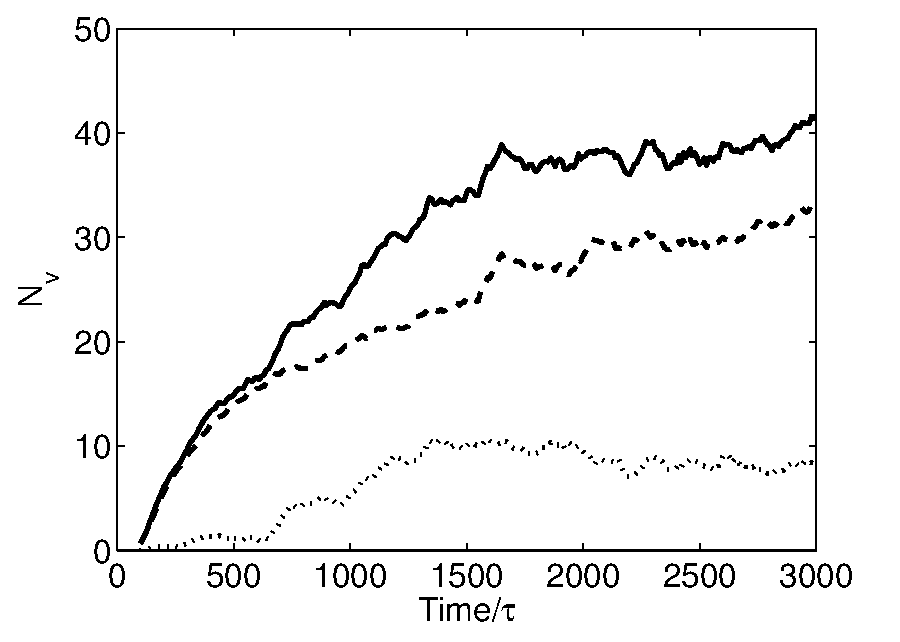
\includegraphics[width=0.45\linewidth]{./afm/figures/nvpn3bw}
%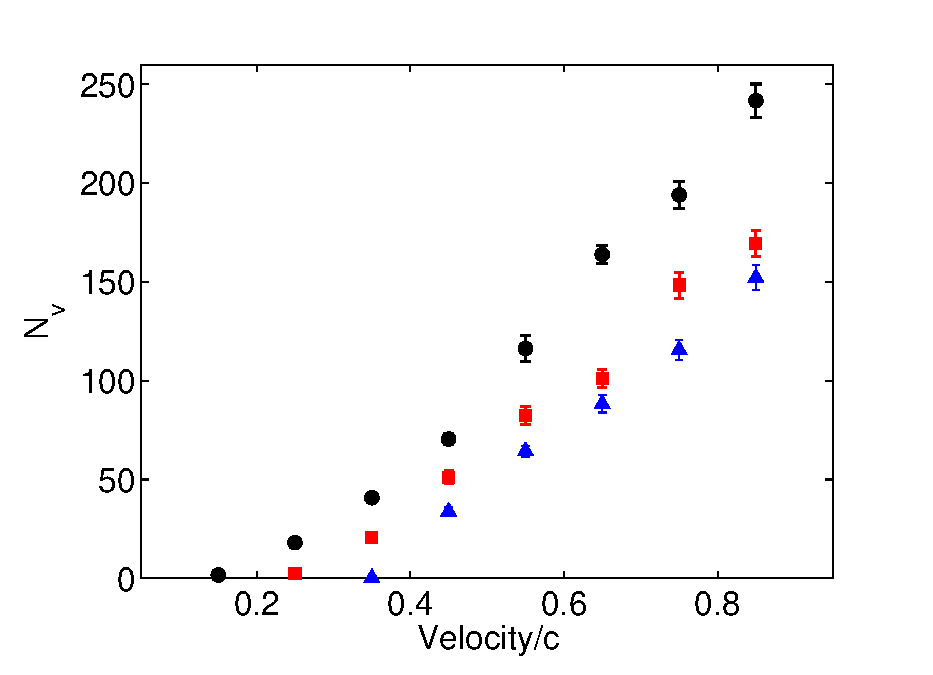
\includegraphics[width=0.45\linewidth]{./afm/figures/nv_v}
%\caption{\label{fig:nvort} (a) Number of vortices produced during $v=0.35c$ flow past the surface.  Shown are the numbers of total %vortices $N_v$ (solid line), positive vortices (dashed line) and negative vortices (dotted line). (b) Final number of vortices $N_v$ as a %function of the flow velocity $v$ for the 2d simulations.  Each data point represents the average of 20 measurements of $N_v$ in the %vicinity of $t=3000\tau$.}
%\end{figure} 

 
\section{Three-dimensional results}
We now move on to focus on the three-dimensional case, modelling the 3D surface by utilising the entire AFM data set. Due to the large computational requirements of a fully 3D numerical simulation of the scale required, only the full height surface (no truncation) for only a few velocities is performed.

\subsection{Vortex nucleation from the surface}
In similarity to the two-dimensional case, in the vicinity of the surface the local fluid speed, $v_{\rm loc}=|{\bf v_{\rm loc}}|$, is enhanced considerably by the surface roughness, with maximum speeds occurring near the tallest mountain. This can be seen through inspection of the local velocities near the surface, shown for several points in time in Figure \ref{fig:velsandvorts} (a-c). Throughtout the simulation the areas of highest velocity occur near the surface prominences seen in Figure \ref{fig:afmsmooth}.

\begin{figure}
  \centering
  \makebox[\textwidth]{
  \begin{minipage}{1.1\textwidth}
  \hspace*{0.75cm}(a) \hspace{4cm}(b) \hspace{4cm}(c)\vspace{-0.5cm}\\
  \begin{tikzpicture}
    \begin{axis}[
        width=0.33\linewidth,
        xlabel={\phantom{$x/\xi$}},
        ylabel=$y/\xi$,
        xmin=-180,
    xmax=180,
    ymin=-180,
    ymax=180,
        major tick length = 0.07cm,
        axis on top,
      major tick length = 0.07cm,
      unit vector ratio=1 1 1,
      ]
      \addplot graphics [xmin=-180,xmax=180,ymin=-180,ymax=180] {afm/vels1.png};
    \end{axis}
  \end{tikzpicture}
   \begin{tikzpicture}
    \begin{axis}[
        width=0.33\linewidth,
        xlabel={$x/\xi$},
        ylabel={},
        xmin=-180,
    xmax=180,
    ymin=-180,
    ymax=180,
        major tick length = 0.07cm,
        axis on top,
      major tick length = 0.07cm,
      unit vector ratio=1 1 1,
      ]
      \addplot graphics [xmin=-180,xmax=180,ymin=-180,ymax=180] {afm/vels2.png};
    \end{axis}
  \end{tikzpicture}
   \begin{tikzpicture}
    \begin{axis}[
        width=0.33\linewidth,
        xlabel={\phantom{$x/\xi$}},
        ylabel={},
        xmin=-180,
    xmax=180,
    ymin=-180,
    ymax=180,
        major tick length = 0.07cm,
        axis on top,
        colorbar style={title={$v_{\rm loc}/c$},text width=0.5em,major tick length = 0.07cm},
      major tick length = 0.07cm,
      point meta min = 0,
      point meta max = 1.6,
      unit vector ratio=1 1 1,
      colorbar,colormap name=invmathot
      ]
      \addplot graphics [xmin=-180,xmax=180,ymin=-180,ymax=180] {afm/vels3.png};
    \end{axis}
  \end{tikzpicture}\\
  \hspace*{0.75cm}(d) \hspace{4cm}(e) \hspace{4cm}(f)\\
  \hspace*{0.02\linewidth}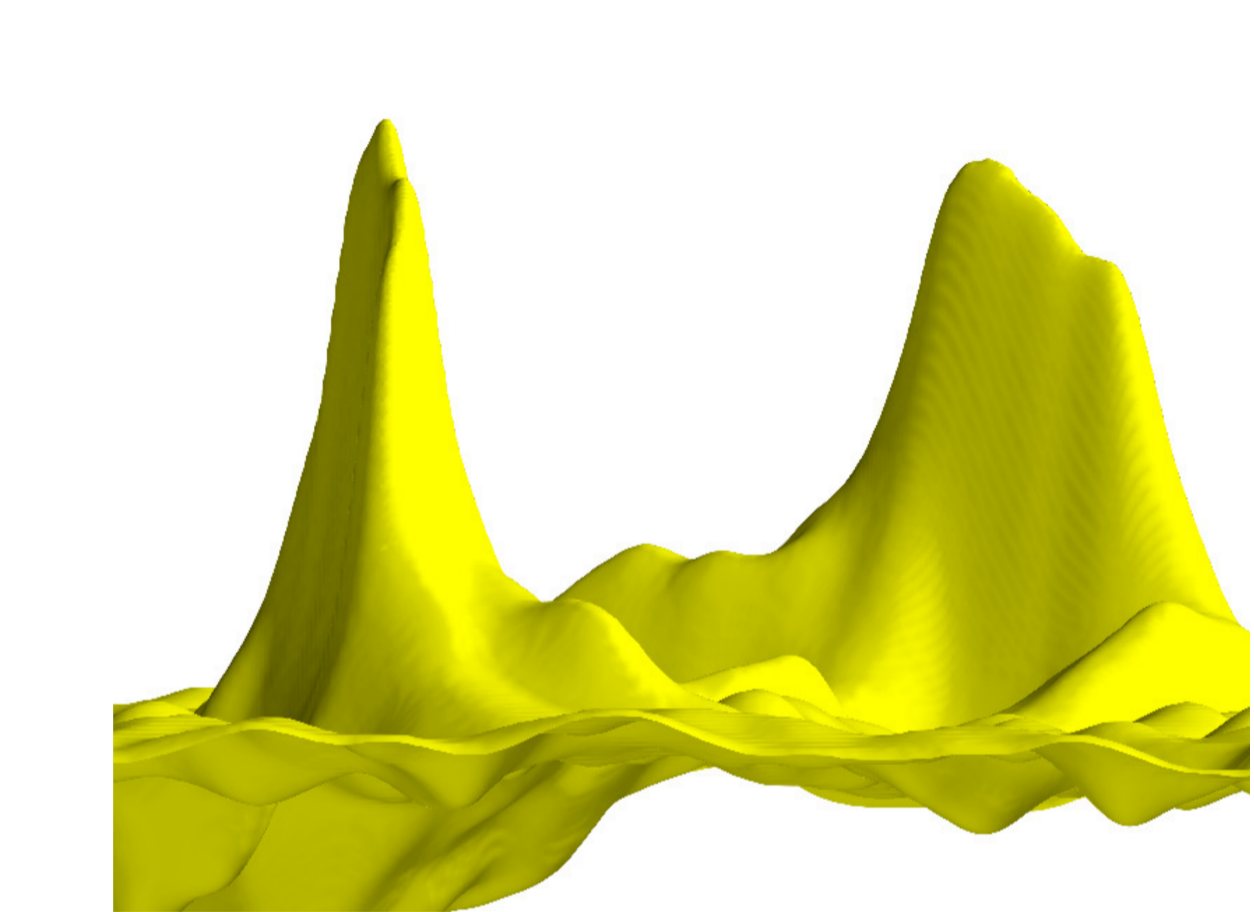
\includegraphics[width=0.3\linewidth]{./afm/afm-sub-2102}
  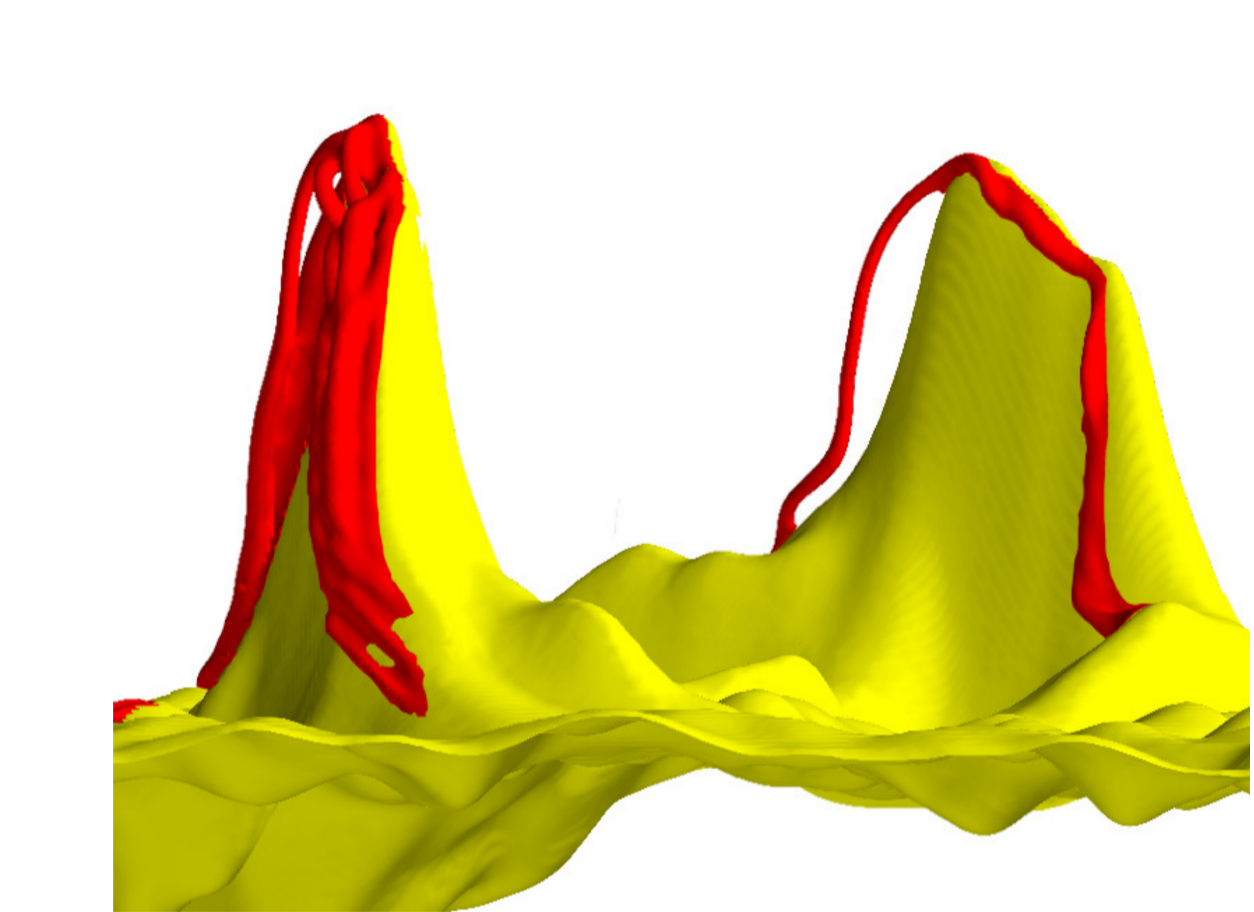
\includegraphics[width=0.3\linewidth]{./afm/afm-sub-3101}
  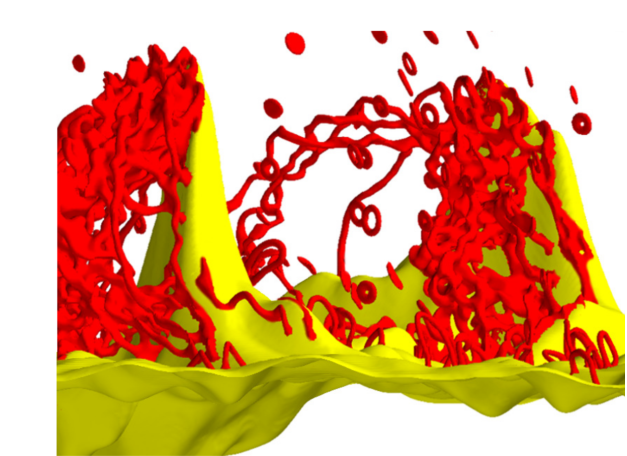
\includegraphics[width=0.3\linewidth]{./afm/afm-sub-10101}
  \end{minipage}
  }
  \caption{\label{fig:velsandvorts}(a-c) Magnitude of the local fluid speed, $v_{\rm loc}=|{\bf v_{\rm loc}}|$, shown in the $xy$-plane and computed just above the surface (where the
density drops to 10\% of the bulk density), at three times $t=20,30,100\,\tau$ with $v=0.6\,c$.  (d-f) Zoomed isosurface plots of density $n({\bf r},t)$ (plotted at 25\%  of the bulk density), showing the surface (yellow) and vortices (red) in the vicinity of the two tallest mountains (view taken along $y$ over the $x$-range $15 \xi \leq x \leq 125 \xi$) at the same times.  %Just prior to vortex nucleation [(left) $t=20 \tau$], the largest fluid speed arises in the vicinity of the highest mountains.  When the fluid speed becomes supercritical at the highest mountains [(middle)$t=30 \tau$], vortex lines becomes nucleated.  At later times [(right)$t=100 \tau$], vortices continue to be shed predominantly by the highest mountains, where the fluid speed continues to be highest.  
%The nucleation vortex loops pass downstream (to the left of the mountains), filling a turbulent layer up to the height of the highest mountain.  This causes a marked downstream spreading of high fluid speed. }
}
 \end{figure} 

As expected, up to a critical imposed velocity, the flow remains laminar and free of vortices.  The critical velocity for vortex nucleation across this particular surface occurs for an imposed flow of $v_c\approx 0.2 c$; this is considerably smaller than, say a hemispherical bump for which $v_c \approx 0.5 c$ \cite{win01},  indicating the significant role of the surface roughness in enhancing the breakdown of laminar flow, similarly to the two-dimensional case. For an increased imposed flow velocity of $v=0.6\,c$, the critical velocity is first exceeded at the highest mountain, leading to nucleation of vortex lines, shown in Figure \ref{fig:velsandvorts} (e), and then by other high mountains on the surface.

Nucleated vortices either peel off the boundary, or, more frequently, slide
down the slopes of the mountains in the form of partially attached vortex loops (carried by the imposed flow). Nucleated vortex loops are of the same circulation and so form clusters (manifesting as partially attached vortex bundles) on the leeward side of the mountains.

The combined velocity field of the vortex bundles along with nucleation of small vortex loops throughout the surface causes an increase and spreading of areas with high local velocity near the surface, visible in Figures~\ref{fig:velsandvorts}(b, c). The velocity field causes vortex stretching and further vortex nucleation, distorting the organised bundles of vortices and small rings into a complex tangle downstream of the mountains. The resulting tangle is continuously fed by further vortices nucleated from the surface. Vortex bundles and the beginnings of such a tangle can be seen in Figure \ref{fig:velsandvorts}(f). The fully developed vortex tangle in the vicinity of the surface is demonstrated in Figure \ref{fig2}.

\subsection{Three-dimensional boundary layer}
\begin{figure}
(a) \hspace{7.2cm}(b)\vspace{-1cm}\\
\begin{center}
  \raisebox{0.8cm}{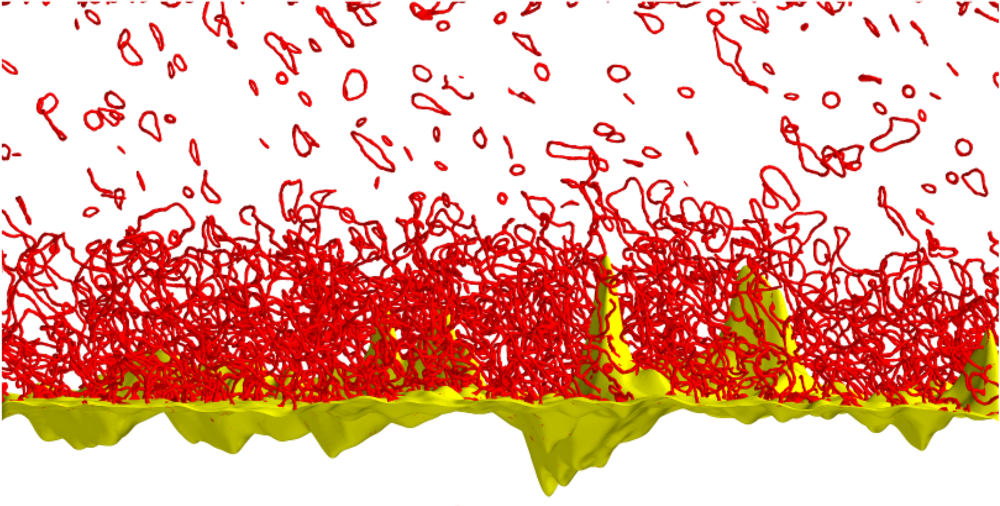
\includegraphics[width=0.5\linewidth]{./afm/fig2-2a}}%
  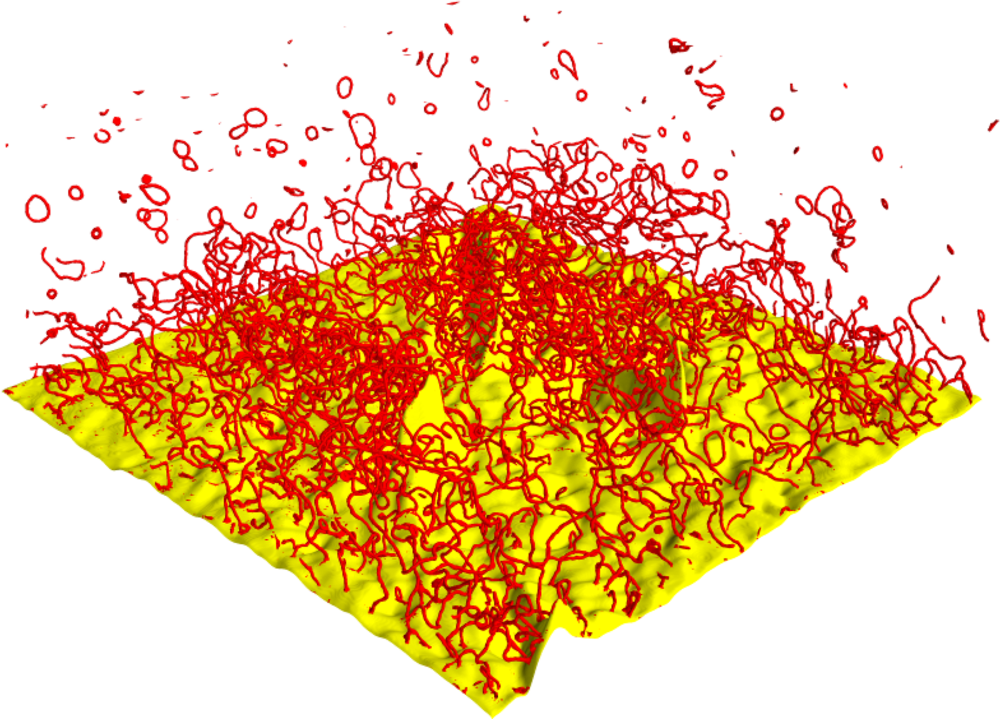
\includegraphics[width=0.5\linewidth]{./afm/fig2-2b}%
\end{center}
\caption{Instantaneous isosurfaces of density $n({\bf r},t)$ 
(plotted at 25\%  of the bulk density) showing the surface (yellow) and vortices (red) for a super-critical flow ($v=0.6 c$) in the saturated 
turbulent regime reached at long times ($t=1220 \tau$).  Notice the turbulent boundary layer up to
approximately the height of the highest mountains and the region
of small vortex rings above it.}
\label{fig2}
\end{figure}
We focus on our 3D simulation with an imposed flow speed of $v=0.6\,c$. For this combination of surface and flow speed, as the number of vortices increases the complex turbulent region of vortex lines remains strongly localised to the vicinity of the surface, up to approximately the height of the highest mountain. The distribution of vortices can be seen to form a distinct layer, visible in the lower half of Figure \ref{fig2} (a). In addition to the visible layer, reconnections due to the interaction of neighbouring vortex lines causes a continuous ejection of vortex rings which spread into the bulk, visible in the upper part of Figure \ref{fig2} (a-b).

The turbulent layer and ejected vortex rings are not isotropic: on average, vortex lines are flattened parallel to plane of the surface and the ejected vortex rings lie more in the $xy$ plane (so that they travel vertically away from the layer). For the slower, but still super-critical, imposed flow with speed $v=0.2\,c$ the turbulent layer still forms with the same height, albeit with reduced density of vortices, generalising the behaviour of the boundary layers that formed in our 2D simulations.

\subsubsection{Vortex line-length density}
As the layer of vortices forms, the vortex line-length in the vicinity of the boundary increases with time at a much faster rate than in the bulk. However, once the layer has covered the entire computational surface, the vortex line-length within the boundary layer approximately saturates. Vortex rings continue to be ejected from the layer, and so the vortex line length in the bulk continues to slowly grow. 

\begin{figure}
  \centering
  \begin{tikzpicture}
    \begin{axis}[ylabel near ticks,xlabel near ticks,
        width=0.6\linewidth,
        height=0.4\linewidth,
        xlabel={$t/\tau$},
        ylabel={$L\xi$},
        xmin=0,
        xmax=1300,
        ymin=0,
        ymax=3e-3,
        xtick pos=left,
        ytick pos=left,
        major tick length = 0.07cm,
        axis on top
      ]
      \addplot[mark=*,thick,blue,line join=round] table[x=t,y=top]{afm/vv_t.dat};
      \addplot[mark=square*,thick,red,line join=round] table[x=t,y=bot]{afm/vv_t.dat};
    \end{axis}
  \end{tikzpicture}
  \caption{\label{fig:vortlinedensdt}Vortex line-density below ($L_0$, red squares) and above ($L_1$, blue circles) the height of $z=100\xi$, approximately the height of the tallest mountain, for a 3D simulation with imposed flow speed of $v=0.6\,c$.} 
  \end{figure}
We quantify this behaviour by monitoring vortex line-density below and above the height of the highest mountain, $L_0$ and $L_1$ respectively. By measuring line-density in this way we are able to ascertain two things. Firstly, we will be able to measure the boundary layer's vortex line-density over time, so as we can say when the layer has saturated. Secondly, we can compare values in the region of the surface and away from the surface, as a measure of the density of the boundary layer compared to the bulk.

We split the computational box in half, with $z<100\xi$ and $z \geq 100\xi$. We first estimate the vortex line-length in each half using the method described in Section \ref{section:linelength}, obtaining the vortex line-lengths for the lower and upper half of the box, $V_0(t)/A$ and $V_1(t)/A$ respectively. Finally the two quantities are used to compute the vortex line-densities $L_0$ and $L_1$ throughout the simulation, shown in Figure \ref{fig:vortlinedensdt}.

We find that both $L_0$ and $L_1$ grow over time as vortex lines are nucleated into the superfluid. $L_0$ quickly grows at early times, and then saturates at a value around $2.4\times 10^{-3}$ at around $t \approx 800$. On the other hand, $L_1$ grows much slower than $L_0$ and shows significantly less vortex line-density throughout the simulation, and does not saturate but instead exhibits a steady growth of vortex line-density throughout, even after $L_0$ has saturated at $t \approx 800$.

These measurements confirm a transient period of fast vortex line-density growth at early times which saturates in the lower half of the computational box, corresponding to the region in the vicinity of the rough surface. In addition, we observe a continuous growth of vortex line-density in the bulk, due to vortex ring formation and emission into the upper half of the computational box. This process is further investigated in Section \ref{sec:vortexmill}.

\subsection{\label{sec:vortexmill}Vortex ring generation through the vortex mill mechanism}
At early times, nucleated vortex lines can form aligned along the flow direction, twisted due to the bundling of vortex lines nucleated at high-frequency. An example of this structure can be seen in the background of Figure \ref{fig:velsandvorts} (f). The twisted vortex lines generate more vorticity which feed into the boundary layer tangle, by spooling small vortex loops though the vortex-mill mechanism envisaged by Schwarz \cite{PhysRevLett.64.1130}. This confirms that, for the AFM surface and an imposed flow of $v=0.6\,c$, the vortex tangle which develops can be interpreted as generated either intrinsically or extrinsically: in both cases vortices nucleate at the highest mountains before filling the layer below.

At later times (due to the modified velocity field by the saturated boundary layer) and for higher imposed flow velocities, the critical velocity is exceeded across greater areas of the surface. However, even after the generation of a considerable vortex tangle, the highest mountains continue to dominate vortex nucleation; here the fluid velocity is always the highest and vortex shedding occurs at the fastest rate. Despite this, we have already seen that the vortex line-density in the vicinity of the surface saturates at late times. To maintain equilibrium, vortex line-length is continuously ejected from the boundary layer by the process of vortex twisting, reconnections, and the formation of vortex rings that detach and travel in the positive $z$ direction; a demonstration of this process is seen in Figure \ref{fig:escapering}. This process provides further evidence of the presence of a vortex mill mechanism in the system, where vortex line-length is injected into the bulk of the superfluid in the form of small rings escaping the boundary layer tangle.
\begin{figure}
(a)\hspace{3.5cm}(b)\hspace{3.5cm}(c)\hspace{3.5cm}(d)\vspace{-0.75cm}\\%
\begin{center}
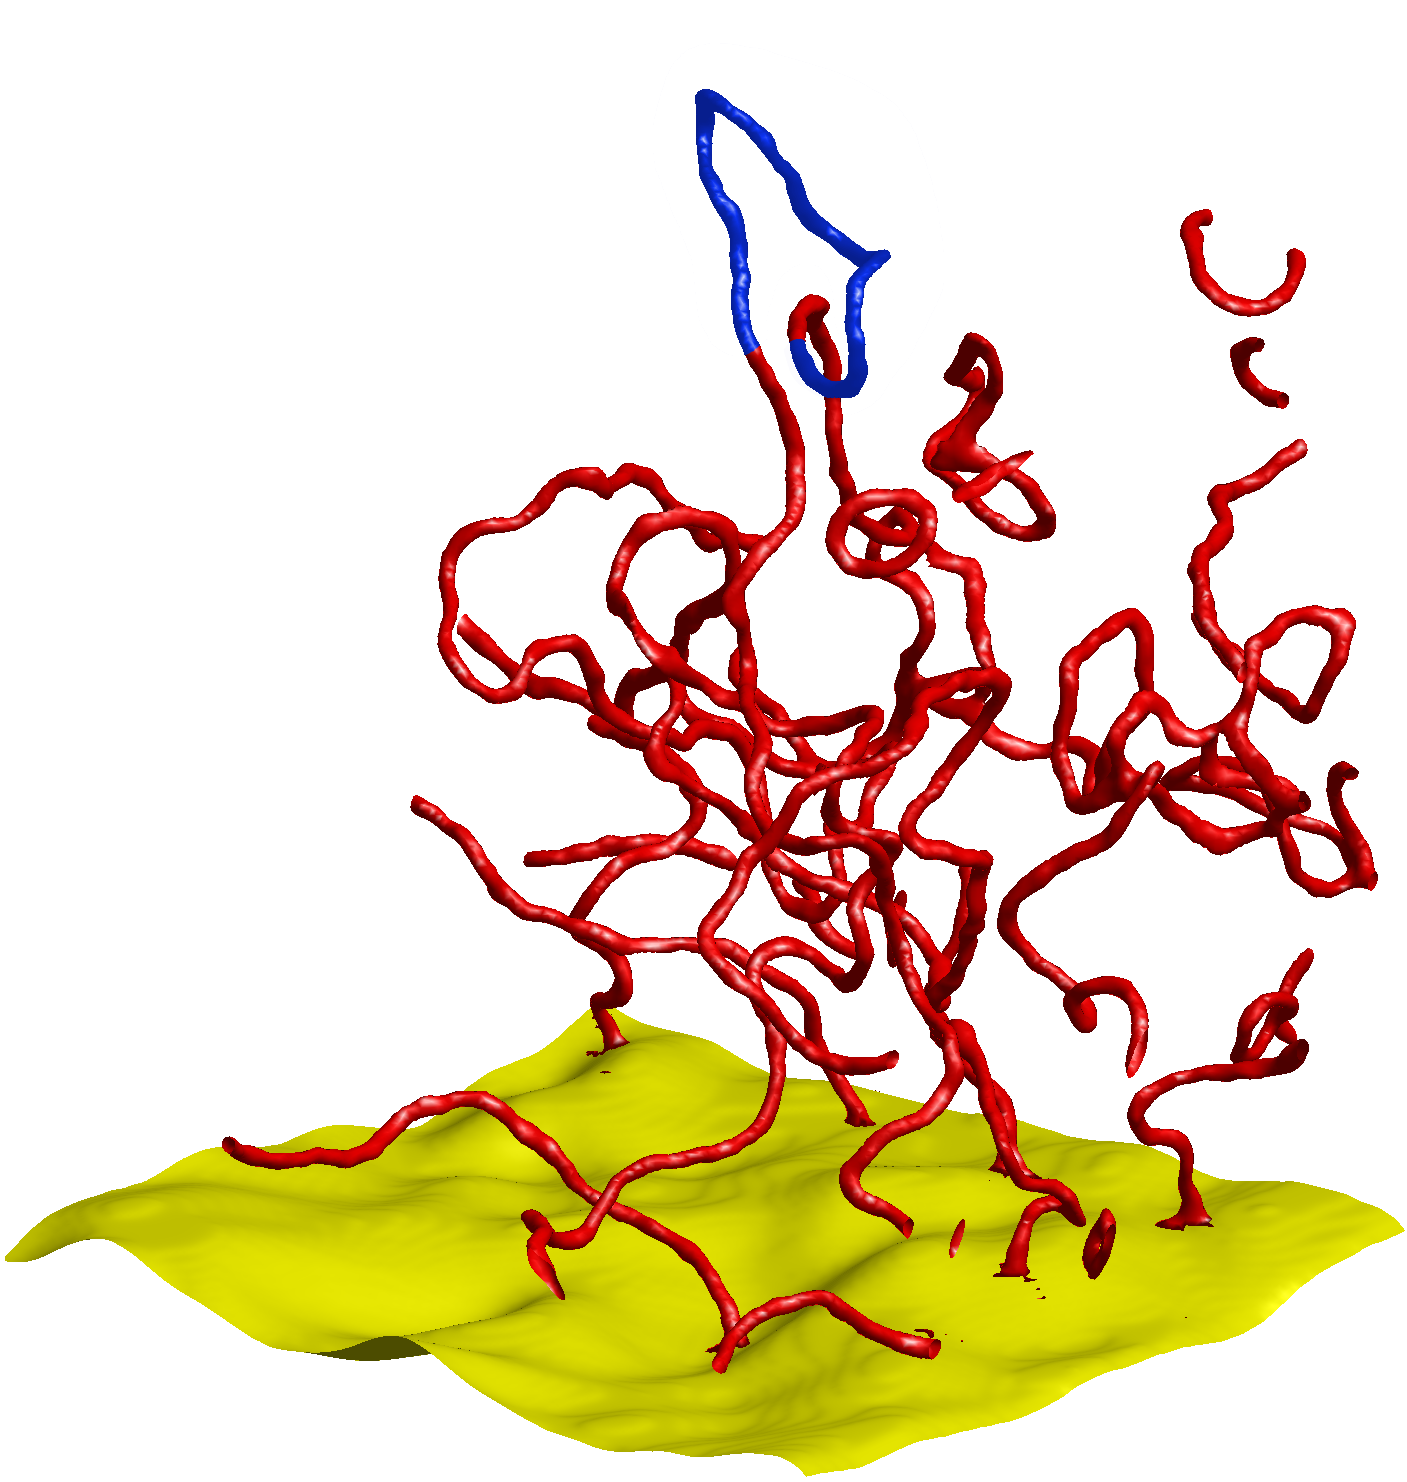
\includegraphics[width=0.25\linewidth]{./afm/mill1}%
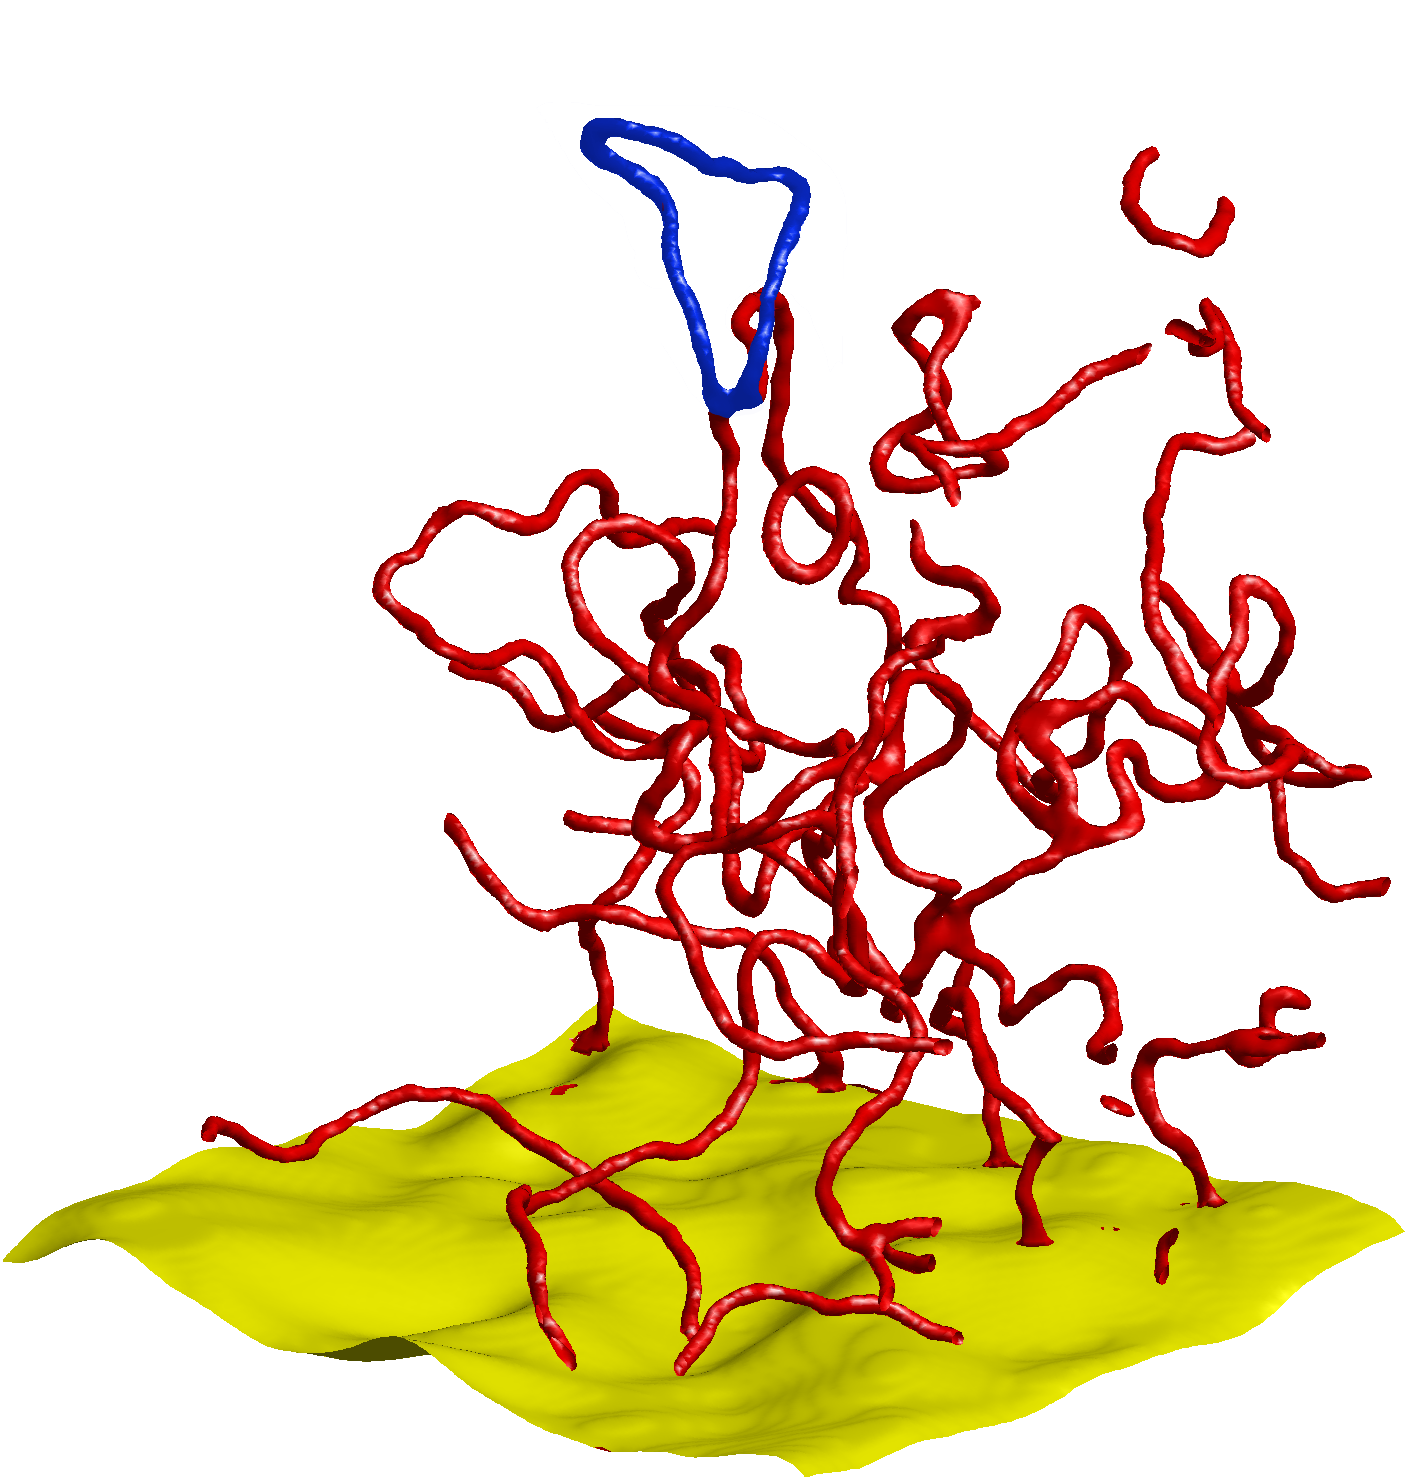
\includegraphics[width=0.25\linewidth]{./afm/mill2}%
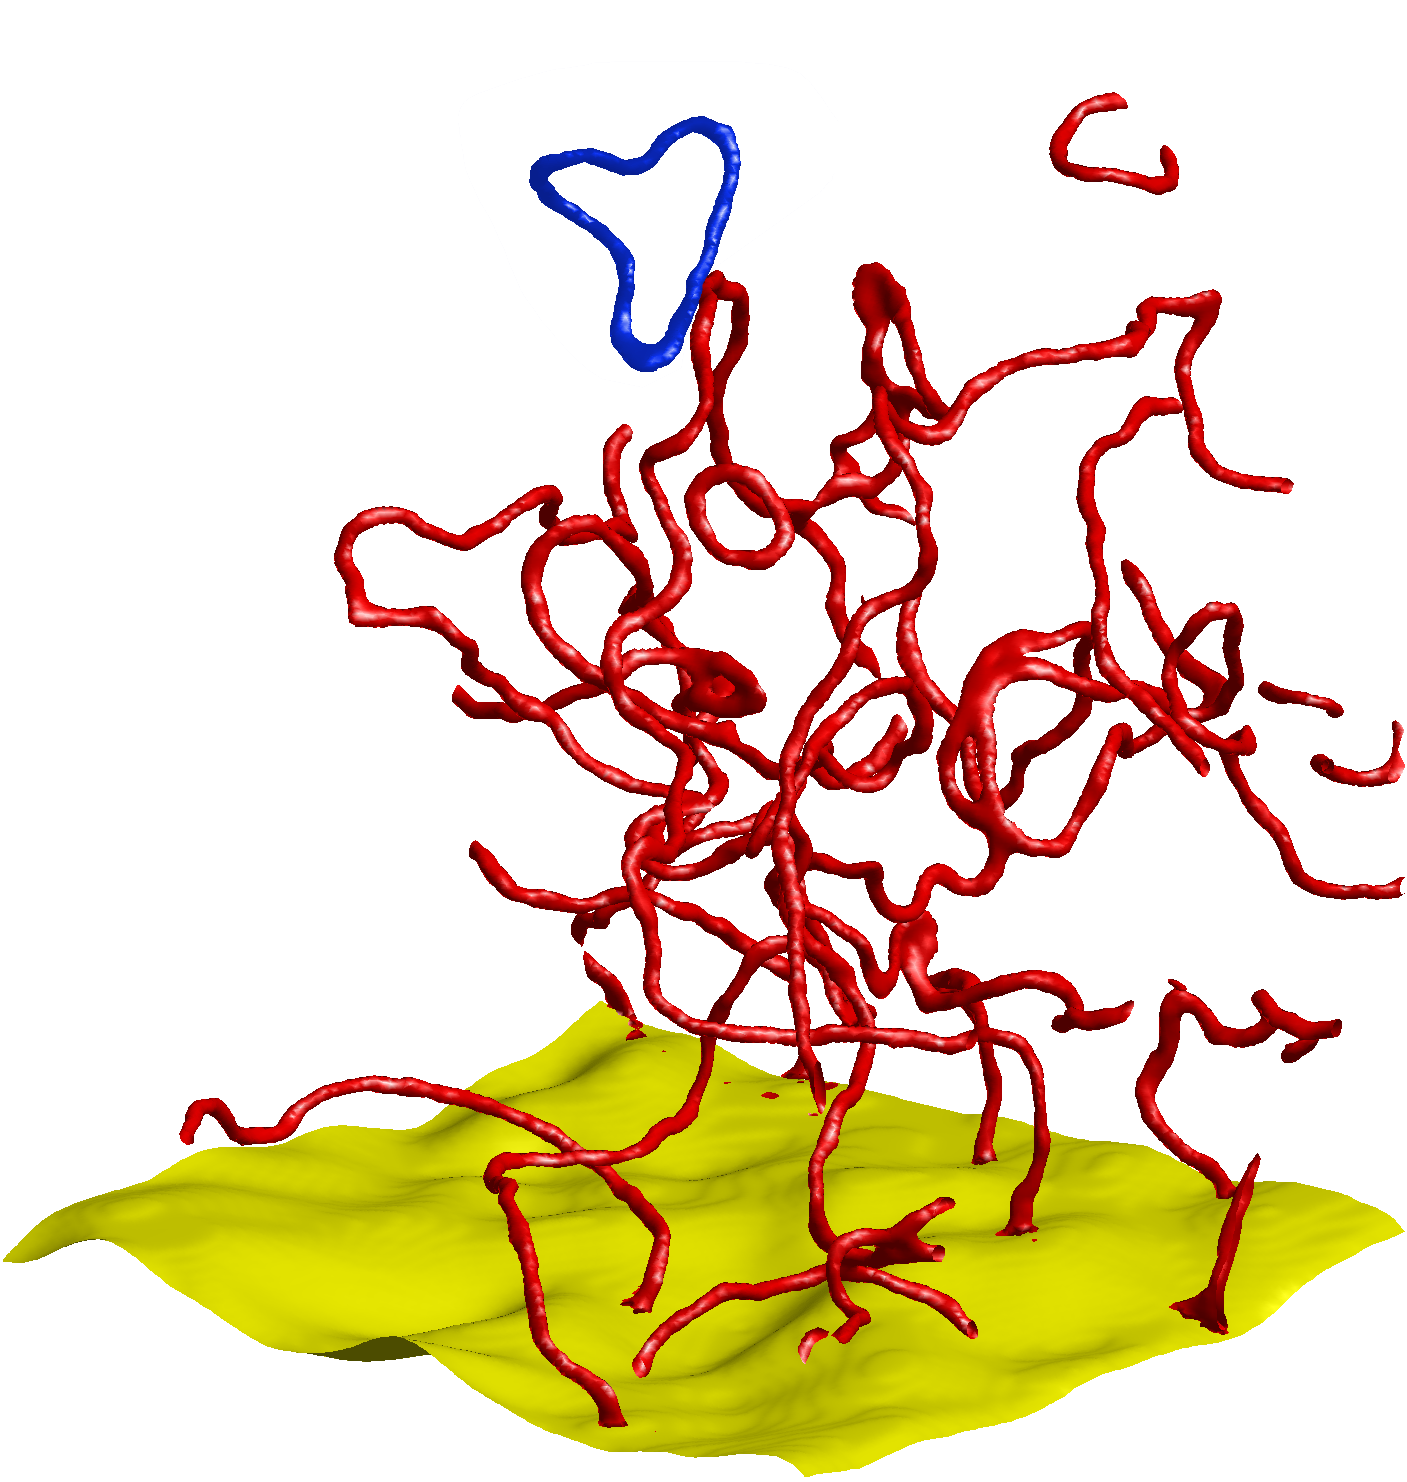
\includegraphics[width=0.25\linewidth]{./afm/mill3}%
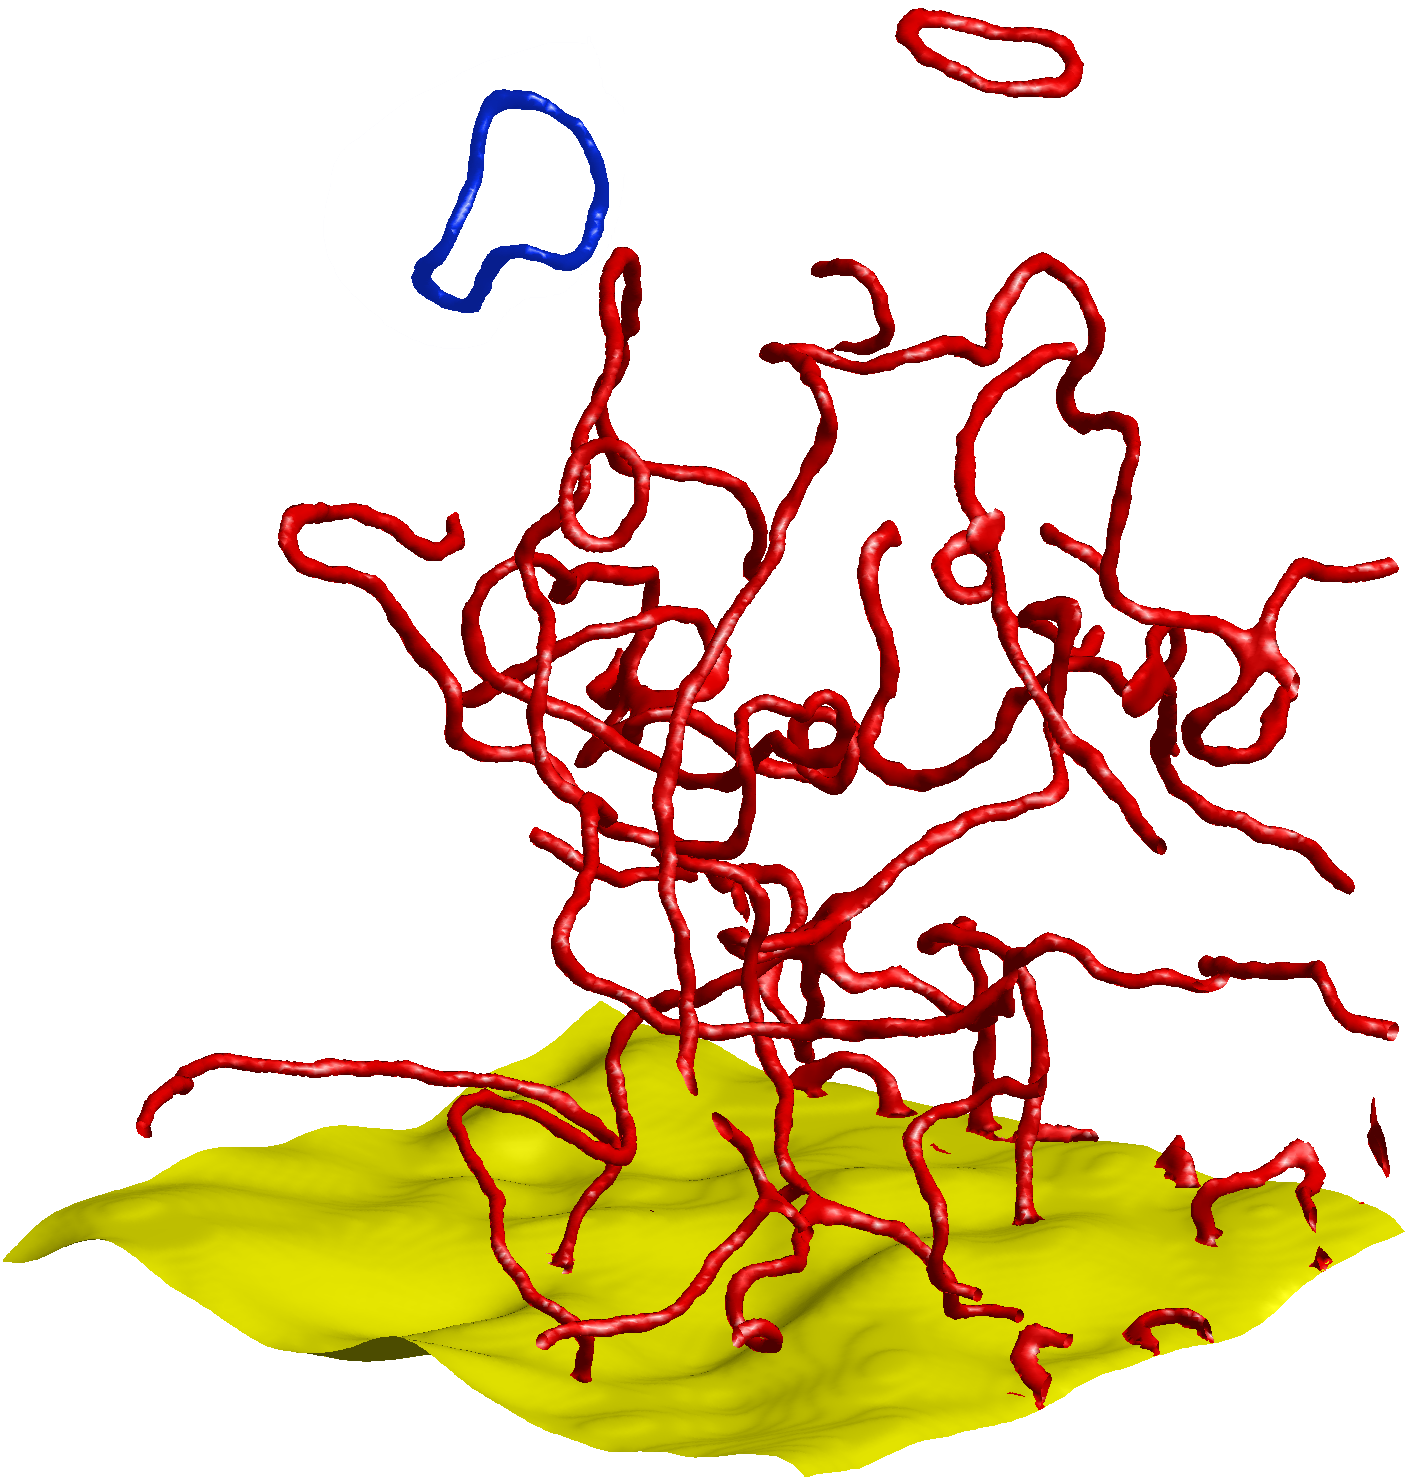
\includegraphics[width=0.25\linewidth]{./afm/mill4}%
\end{center}
\caption{Instantaneous isosurfaces of density $n({\bf r},t)$ 
(plotted at 25\%  of the bulk density) showing the rough surface (yellow) and vortex lines (red) in the saturated regime at times $t=730,740,750,770\,\tau$ and with $v=0.6\,c$. The view is of the region $120\xi<x<196\xi$, $48\xi<y<124\xi$, $20\xi<z<160\xi$. Highlighted in blue is an escaping vortex ring (originating from the tangle) that later travels in the positive $z$ direction and into the bulk of the fluid.}
\label{fig:escapering}
\end{figure}

\subsubsection{Velocity profile}
We further explore the turbulent boundary layer by measuring the local velocity as a function of distance, so as to obtain a velocity profile. We measure the quantity 
\begin{equation}
  v_{\rm xy}(z) = \langle v_{\rm loc}({\bf r}) \rangle_{\rm xy},
\end{equation}
where $\langle v_{\rm loc}({\bf r}) \rangle_{\rm xy}$ denotes averaging of the local fluid speed in the $xy$ plane. We measure $v_{\rm xy}(z)$ for all $z$ using an average of 10 snapshots at times $1130<t/\tau<1220$ (so that we measure the turbulent saturated regime). The resulting quantity $v_{\rm xy}(z)$ is a measurement of the typical local speed of the fluid flow at the height of $z$. We for our simulation with $v=0.6\,c$, we find three regions in the profile of $v_{\rm xy}(z)$.

In the region $100\xi \lesssim z \lesssim 200\xi$, the local flow speed is $v_{\rm xy}(z)\approx0.6$, showing that the fluid velocity is unaffected by the rough surface at heights of more than the height of the tallest mountain.

In the region $40 \lesssim z \lesssim 100\xi$ the presence of vortices near the surface creates a velocity field that counteracts the imposed flow velocity. The overall effect is to slow the typical flow speed the closer to the surface that it is measured, in analogy to a viscous boundary layer in classical fluids.

In the region $0 \lesssim z \lesssim 40\xi$ most of the computational volume is below the surface, and so only the fluid in the valleys is computed as part of the average. In this region the typical speed of the flow rapidly drops to almost zero.

\begin{figure}
  \centering
  \begin{tikzpicture}
   \begin{axis}[ylabel near ticks,xlabel near ticks,
        width=0.5\linewidth,
        height=0.5\linewidth,
        xlabel=$x/\xi$,
        ylabel=$\phantom{y/\xi}$,
        xtick pos=right,
        ytick pos=right,
        yticklabels={,,},
        ytick={},
        xmin=-180,
        xmax=180,
        ymin=0,
        ymax=195,
        major tick length = 0.07cm,
        axis on top,
      ]
      \addplot graphics [xmin=-200,xmax=200,ymin=0,ymax=98] {afm/shadow.png};
    \end{axis}
    \begin{axis}[ylabel near ticks,xlabel near ticks,
        width=0.5\linewidth,
        height=0.5\linewidth,
        xlabel={$v_{\rm xy}/c$},
        ylabel={$z/\xi$},
        xmin=0,
        xmax=0.8,
        ymin=0,
        ymax=195,
        xtick pos=left,
        ytick pos=left,
        major tick length = 0.07cm,
        axis on top
      ]
      \addplot[mark=none,ultra thick,blue,line join=round] file {afm/vels_z.dat};
    \end{axis}
  \end{tikzpicture}
  \caption{Typical local flow speed (lower abscissa) at various heights above the surface of the wire, averaged over $10$ points in time, at $1130<t/\tau<1220$ and with $v=0.6\,c$. For comparison, a 2D sample of the 3D surface ($y=0.1\,\mu$m, demonstrating one of the tallest surface features) is shown in grey (upper abscissa).} 
  \end{figure}

\section{Conclusions}
In conclusion, we have modelled superflow over a real surface region of a thin NbTi ``floppy wire'' used in helium II experiments and imaged via Atomic Force Microscopy. We have used the zero temperature GPE to numerically simulate a superfluid flow with the profile of the wire inserted using a potential term, obtaining numerical results in both 2D and in 3D.

We have performed 2D simulations and explored the parameter space of surface roughness (modified by truncation of the `roughest' features in the wire) and flow velocity (imposed via a frame shift in the governing equation). For all roughness we have observed the formation of a 2D `boundary layer' at certain velocities exceeding the critical velocity, consisting of a collection of quantum vortices that remain in the vicinity of the surface. We find that imposing an even higher velocity destroys the boundary layer behaviour. Our large scale 3D simulations also confirm that, for at least one set of parameters, the formation of the boundary layer generalises to three dimensions. We have shown the vortex line-density saturates over time in the layer, and have demonstrated a qualitatively similar boundary layer velocity profile as those seen in classical viscous fluids.

Our findings are a surprising result, in fluid dynamics boundary layers usually arise from viscous forces, which in superflow at absolute zero are completely absent.  These findings further illustrate the deep analogies between classical and quantum fluids.

Our results suggest that in current helium II experiments the walls of channels which confine the flow of superfluid liquid helium and the surfaces of moving objects such as wires, grids, propellers, spheres may be covered by a thin `superfluid boundary layer' consisting of vortex loops and rings. The experimental implications of `superfluid boundary layers` on macroscopic
observables need to be investigated.  This should particularly stimulate experiments in $^3$He-B, where, due to relative large healing length, it is possible to study flows with controlled surface height roughness. Our results could also be interpreted and potentially observable in the context of quasi-two-dimensional atomic BEC experiments, where recent work has enabled dynamic arbitrarily shaped obstacles, `painted' with blue-detuned laser light \cite{Henderson09}.
\end{chapter}


%\section{\label{section:sfwire} Superfluid wire experiments}
%Developments in flow visualization at very low temperatures
%\cite{Guo2014,Fisher2014} have
%driven recent progress in the turbulence in superfluid $^4$He and
%$^3$He-B. Experiments and theory have highlighted effects
%such the existence of classical and
%nonclassical turbulent regimes \cite{WalmsleyGolov2008}, and
%energy transfer over length scales, both
%direct \cite{Barenghi2014} and inverse
%\cite{WalmsleyTompsett2013,Baggaley2014}.
%At the same time, improvements in the generation, observation and control of quantum
%vortices in atomic Bose--Einstein condensates\cite{Henn,Freilich2010,aioi11,neely_bradley_13,kwon_moon_14}
%has added a character of interdisclinarity to the study of
%turbulence in quantum fluids.

%In many superfluid helium experiments \cite{VinenSkrbek2008}, turbulence
%is generated by moving grids \cite{Davis2000},
%wires \cite{Guenault1986,brad05,Bradley2011,Fisher2001,goto08},
%forks \cite{Blaauwgeers2007,Bradley2012} or spheres \cite{Schoepe1995}.
%Although macroscopically polished, the surface of these objects is
%rough on the length scale of the superfluid vortex core, which is of
%the order of $10^{-10}~\rm m$ in $^4$He
%and $10^{-8}~\rm m$ in $^3$He.  As an example, Fig.~\ref{fig:afmimg}(a) is an atomic force microscope (AFM) image showing the microscopic detail on the surface of a  single--core NbTi `floppy' wire used for generating superfluid turbulence  \cite{Bradley2011}.  Note the appearance of an elongated scratch, typical of such wires.  No direct flow visualization is available on these microscopic length scales and, as such, 
%superflow in the presence of walls remains poorly understood. In principle, the superfluid boundary conditions should
%be straighforward.
% the simplest case of a boundary at rest, the superfluid velocity
%component which is perpendicular to the boundary must be equal to
%zero at the boundary, while the tangential component can slip.
%In practice, nucleation of quantum vorticity complicates
%this idealized Eulerian picture.

%The established theoretical approaches used to successfully describe
%homogeneous superfluid turbulence away from boundaries can falter in the presence of realistic boundaries.
%First consider the vortex filament method of Schwarz
%\cite{Schwarz,Hanninen-PNAS}. Its application to relatively simple and smooth
%boundaries, such as spheres \cite{Hanninen-sphere,Kivotides-sphere} and
%hemispheres \cite{Schwarz-bump}, has proved
%cumbersome due to the complex system of images which is required.
%Its starting assumption, that the vortex core
%is infinitesimally smaller than any other length scale, makes it
%unsuitable for realistic boundaries of roughness comparable to
%the vortex core size.  Moreover Schwarz's approach requires arbitrarily seeding
%vortex loops, because it does not account for vortex nucleation.
%Another approach which suffers similar difficulties \cite{Henderson} is
%the two--fluid Hall--Vinen--Bekarevich--Khalatnikov (HVBK)
%equations \cite{Salort2011,Salort2012}. Moreover, the HVBK equations are coarse--grained over
%length scales larger than the average vortex separation, hence the
%boundary conditions require further assumptions or the introduction of
%unknown sliding/pinning parameters.

%A practical dynamical model of superflow near boundaries of arbitrary
%shape which is powerful enough to describe vortex nucleation is
%the Gross--Pitaevskii equation (GPE) \cite{RobertsBerloff}.  While the GPE is an accurate quantitative description of atomic condensates, it provides only a qualitative model of superfluid helium.  Frisch {\it et al.} pioneered the GPE approach by simulating superflow past a cylinder, observing vortex pair nucleation above a critical flow speed \cite{frisch92}.  Subsequent GPE-based works have further elucidated vortex generation past a cylinder \cite{nore93,jma99,saito10}, as well as spheres and half-spheres \cite{winiecki99}, and elliptical objects \cite{stagg_parker_14}.    Nevertheless, at this stage of investigation, the GPE is the optimum tool 
%to gain physical insight into the flow of a superfluid over
%rough surfaces typical of experiments.

%Our numerical approach is to first obtain the stationary solution for the static fluid $(v=0)$, achieved via imaginary time propagation of the GPE \cite{Minguzzi2004}.  From this initial condition the GPE is then propagated in real time, with the fluid speed $v$ ramped up smoothly from zero up to its required value.

  \part{Appendix}
  \appendix
  \begin{chapter}{Detailed Derivations\label{app:App2}}
\section{\label{appsection:rk4deriv} Derivation of the Runge-Kutta scheme}
Presented here is the derivation of the explicit second-order Runge-Kutta scheme. The ideas and methods easily extend to the forth-order scheme used in this thesis, but in the interests of brevity the entire proof will be given to second order, with the relevant forth order extensions clearly noted.
Let an initial value problem be specified as
\begin{align*}
  \psi'(t) &= f(\psi(t),t),\hspace{0.25in}\psi(t_0) = \psi_0,
\end{align*}
where $t_n = nh$, $h$ is a chosen step size, and $f(\psi(t),t)$ is known. The aim of the scheme is to estimate some $\psi(t_m)$ from the known $\psi(t_0)$ through the application of a single numerical step of size $h$, $m$ times.

For a single application of the numerical step we attempt to find the unknown value of $\psi(t_{n+1})$, which can be written,
\begin{align*}
\psi(t_{n+1}) &= \psi(t_n) + \left[ \psi(t_{n+1}) - \psi(t_n) \right]\\
          &= \psi(t_n) + \int_{t_n}^{t_{n+1}}\!\!f\left(\psi(\tau),\tau\right)\,{\rm d}\tau.
\end{align*}
We now decide to approximate the (difficult to calculate) integral $\int_{t_n}^{t_{n+1}}\!\!f\left(\psi(\tau),\tau\right)\,{\rm d}\tau$ using quadrature, leading to the modified expression,
\begin{equation*}
\psi(t_{n+1}) \approx \psi(t_n) + h\sum\limits_{i=1}^N \omega_i f(t_n+h\nu_i,\psi(t_n+h\nu_i)),
\end{equation*}
where $N$ is the order of the numerical scheme, $\omega_i$ are weights and $\nu_i$ are locations in time positioned between $t_n$ and $t_{n+1}$ inclusive. In this second-order derivation we take $N=2$, a forth-order scheme would alternatively require $N=4$.

We take the first temporal point to be $\nu_1=0$, so that the first term in the sum is
\begin{equation*}
k_1 = hf(t_n,\psi(t_n)).
\end{equation*}
We can then easily calculate the value of $k_1$. A single step in Euler's method tells us that $\psi(t_n+h\nu_2) \approx h\nu_2f(t_n,\psi(t_n))$ and so we write $k_2$ in a form containing $k_1$,
\begin{equation*}
k_2 = hf(t_n+h\nu_2,\psi(t_n+h\nu_2)) \approx hf(t_n+\nu_2h,\psi(t)+\nu_2k_1).
\end{equation*}
For a forth order scheme we would then introduce $k_3$ and $k_4$, following the same methods of writing $k_i$ in previous terms up to $k_{i-1}$. To second order, the quadrature formula becomes
\begin{equation}
\psi(t_{n+1}) \approx \psi(t_n) + \omega_1k_1 + \omega_1k_2.
\end{equation}\label{eq:rka1}
However, note that we still must derive values for the quantities $\nu_{i>1}$ and $\omega_i$.

Consider the Taylor expansion,
\begin{equation*}
\psi(t+h) = \psi(t) + h\psi'(t) + \frac{h^2}{2}\psi''(t) + \cdots,
\end{equation*}
where for the full forth-order derivation, further higher order terms are also considered. We substitute this expansion into the left hand side of Equation \ref{eq:rka1}, which leads to
\begin{equation}
\psi(t_n) + h\psi'(t_n) + \frac{h^2}{2!}\psi''(t_n) + \mathcal{O}(h^3) \approx \psi(t_n) + \omega_1k_1 + \omega_2k_2.
\end{equation}\label{eq:rka2}
Note that
\begin{align*}
\psi'(t_n)  &= f,\\
\psi''(t_n) &= \frac{\partial f}{\partial t} + f\frac{\partial f}{\partial \psi},
\end{align*}
by the definition of $\psi'(t)$ and the total derivative, and where the arguments of $f(t_n,\psi(t_n))$ have been suppressed for notational ease. We then substitute the expressions for $\psi'(t_n)$, $\psi''(t_n)$, $k_1$ and $k_2$ into Equation \ref{eq:rka2},
\begin{equation}
hf + \frac{h^2}{2}\left(\frac{\partial f}{\partial t} + f\frac{\partial f}{\partial \psi}\right) + \mathcal{O}(h^3) = \omega_1hf + \omega_2hf(t_n+\nu_2h,\psi(t)+\nu_2k_1).
\end{equation}\label{eq:rka3}

Now consider the Taylor expansion,
\begin{equation*}
f(t+h,\psi+g) = f(t,\psi) + h\frac{\partial f(t,\psi)}{\partial t} +g\frac{\partial f(t,\psi)}{\partial \psi} + \cdots,
\end{equation*}
where for the full forth-order derivation, further higher-order terms are also considered. We substitute this expansion into Equation \ref{eq:rka3}, including terms up to the required order, and find
\begin{equation}
hf + \frac{h^2}{2!}\left(\frac{\partial f}{\partial t} + f\frac{\partial f}{\partial \psi}\right) + \mathcal{O}(h^3) = \omega_1hf + \omega_2\left( hf + \nu_2h^2 \frac{\partial f}{\partial t} + \nu_2h^2f\frac{\partial f}{\partial \psi} \right)+ \mathcal{O}(h^3).
\end{equation}\label{eq:rka4}
By equating terms on both the right hand side and left hand side of Equation \ref{eq:rka4}, we find that for the second-order Runge-Kutta scheme the following equivalences are required for consistency,
\begin{align*}
\omega_1 + \omega_2 = 1,\\
\nu_2\omega_2 = \frac{1}{2}.
\end{align*}
For the forth-order scheme, more but similar equivalences are required for consistency. The canonical choice for the second-order Runge-Kutta methods is
$\nu_2=1$ and $\omega_1 = \omega_2 = 1/2$. The scheme can then be directly written down,
\begin{equation}
\psi(t_{n+1}) = \psi(t_n) + \frac{k_1}{2} + \frac{k_2}{2} + \mathcal{O}(h^3),
\end{equation}
where $k_1 = hf(t_n,\psi(t_n))$ and $k_2 = hf(t_n+h,\psi(t)+k_1)$.

When this proof outline is followed with $N=4$, the forth-order Runge-Kutta scheme can be found,
\begin{equation}
    \psi(t_{n+1}) = \psi(t_n) + \frac{k_1}{6}+ \frac{k_2}{3}+ \frac{k_3}{3} + \frac{k_4}{6} + \mathcal{O}(h^5),
\end{equation}
where
\begin{equation*}
\begin{split}
    k_1 &= hf(t_n,\psi(t_n)),\\
    k_2 &= hf(t_n+\frac{h}{2},\psi(t_n)+\frac{k_1}{2}),\\
    k_3 &= hf(t_n+\frac{h}{2},\psi(t_n)+\frac{k_2}{2}),\\
    k_4 &= hf(t_n+h,\psi(t_n)+k_3).
\end{split}
\end{equation*}

\section{\label{appsection:gpeqft} Derivation of the Gross-Pitaevskii Equation}
This section derives the GPE following the methodology outlined in \cite{0953-4075-41-20-203002}. We begin by revisiting the quantum field theory formalism used to describe a many-body quantum system \cite{fetter1971quantum}. Such a system is described by an $N$-body wavefunction, $\tilde{\upPsi}(\mathbf{r}_1...\mathbf{r}_N,t)$ which obeys the famous Schr\"odinger equation
\begin{equation}
i \hbar\frac{\partial}{\partial t}\tilde{\upPsi}(\mathbf{r}_1...\mathbf{r}_N,t) = \hat{H}\tilde{\upPsi}(\mathbf{r}_1...\mathbf{r}_N,t),
\label{eq:gpeqftscho}
\end{equation}
where $\mathbf{r}_i$ describes the coordinates of the $i$th body. Consider a closed system containing a dilute, weakly interacting Bose gas of $N$ atoms. Such a system would be described by $\tilde{\upPsi}(\mathbf{r}_1...\mathbf{r}_N,t)$, with a Hamiltonian of the form 
\begin{equation}
\hat{H} = \sum_{k=1}^N\hat{h}_0(\mathbf{r}_k,t) + \frac{1}{2}\sum_{k,l=1}^N \hat{V}(\mathbf{r}_k,\mathbf{r}_l).
\label{eq:gpeqfthamil}
\end{equation}
Here $\hat{h}_0(\mathbf{r},t) = -\frac{\hbar^2}{2m}\nabla^2+V_{\mathrm{ext}}(\mathbf{r},t)$ is a contribution arising from the effects of a single particle in an external potential. We assume in the dilute gas all interactions are binary, and so the second term arises from collisions between 2 atoms. The factor of $\frac{1}{2}$ ensures the effects are only counted once over the entire sum.

We now reformulate this system in a different representation, using the so called `occupation number' orthonormal basis $\ket{n_1...n_\infty}$. This basis arises from the observation that multiple particles sharing an energetically accessible state are indistinguishable. Instead we consider only the number of particles in each state $i$ and denote this $n_i$. Such states often correspond to states with fixed energy $\varepsilon_i$. While the number of states are infinite, our system contains a fixed number of bosons, $N$, implying that there are at most $N$ states occupied.

The wavefunction is mapped into the `occupation number' basis via
\begin{equation*}
\tilde{\upPsi}(\mathbf{r}_1...\mathbf{r}_N,t) \rightarrow \ket{\tilde{\upPsi}(t)}=\sum_{n_1...n_\infty} c(n_1...n_\infty,t)\ket{n_1...n_\infty},
\end{equation*}
with appropriately chosen complex coefficients, $c(n_1...n_\infty,t)$. The values $c$ must follow the particle statistics rules (e.g. for bosons, must be symmetric under swapping of quantum numbers) and be normalised so that the probabilities correctly sum to one. We find that for our bosons,

\begin{equation*}
\int|\tilde{\upPsi}|^2~d\mathbf{r}=1 \Rightarrow \sum_{n_1...n_\infty}|c(n_1...n_\infty,t)|^2\frac{N!}{n_1!...n_\infty!} = 1.
\end{equation*}

In this formulation, note that the state vectors $\ket{n_1...n_\infty}$ are time-independent, and the evolution of the system is entirely encoded in the values of $c(n_1...n_\infty,t)$. As part of the overall picture, we also must describe the movement of bosons between different states or energy levels. It is convenient to visualise this as the simultaneous destruction of a particle in state $j$ and creation of a particle in state $i$, described mathematically using the single particle annihilation and creation operators \cite{schiff1968},
\begin{align*}
&\hat{a}_j\ket{n_1...n_i...n_j...n_\infty} = \sqrt{n_j}\ket{n_1...n_i...n_j-1...n_\infty},\\
&\hat{a}^\dagger_i\ket{n_1...n_i...n_j...n_\infty} = \sqrt{n_i+1}\ket{n_1...n_i+1...n_j...n_\infty},
\end{align*}
which satisfy the bosonic commutation relations,
\begin{equation*}
[\hat{a}_i,\hat{a}_j^\dagger]=\delta_{ij}\hspace{0.5in}[\hat{a}_i,\hat{a}_j]=[\hat{a}_i^\dagger,\hat{a}_j^\dagger]=0.
\end{equation*}
Any single particle changing states can now be described through these operators; a particle moving from state $j$ to state $i$ is described using a single annihilation operator and a single creation operator through the product $\hat{a}_i^\dagger\hat{a}_j$. Similarly, as we decided to simplify the system by considering a dilute gas where all interactions are binary collisions, all interactions can be described by two particles changing state, using the product $\hat{a}_i^\dagger\hat{a}_k^\dagger\hat{a}_j\hat{a}_l$. Using these tools and ideas, the original description in Equations \ref{eq:gpeqftscho} and \ref{eq:gpeqfthamil} is now written

\begin{equation*}
i \hbar\frac{\partial}{\partial t}\ket{\tilde{\upPsi}} = \hat{H}\ket{\tilde{\upPsi}},
\label{eq:gpeqftsecscho}
\end{equation*}
with the Hamiltonian
\begin{equation}
\hat{H} = \sum_{ij}\bra{i}\hat{h}_0\ket{j}\hat{a}_i^\dagger\hat{a}_j + \frac{1}{2}\sum_{ijkl} \bra{ik}\hat{V}\ket{jl}\hat{a}_i^\dagger\hat{a}_k^\dagger\hat{a}_j\hat{a}_l,
\label{eq:gpeqftsechamil}
\end{equation}
where
\begin{align*}
&\bra{i}\hat{h}_0\ket{j} = \int \phi_i^*(\mathbf{r})\hat{h}_0\phi_j(\mathbf{r})~d\mathbf{r},\\
&\bra{ik}\hat{V}\ket{jl} = \frac{1}{2}\left [ (ik|\hat{V}|jl) + (ik|\hat{V}|lj) \right ],\\
&(ik|\hat{V}|jl) = \iint \phi_i^*(\mathbf{r})\phi_k^*(\mathbf{r}')\hat{V}(\mathbf{r}-\mathbf{r}')\phi_l(\mathbf{r}')\phi_j(\mathbf{r})~d\mathbf{r}'d\mathbf{r}.
\end{align*}
For further convenience we introduce the so-called Bose field operators
\begin{align*}
&\hat{\upPsi}(\mathbf{r},t) = \sum_i \hat{a}_i(t)\phi_i(\mathbf{r},t),\\
&\hat{\upPsi}^\dagger(\mathbf{r},t) = \sum_i \hat{a}^\dagger_i(t)\phi_i(\mathbf{r},t),
\end{align*}
which can be thought of as operators that represent the addition or removal of a particle at time $t$ and location $\mathbf{r}$. As with the annihilation and creation operators, the Bose field operators also satisfy the commutation relations,
\begin{equation}
[\hat{\upPsi}(\mathbf{r},t),\hat{\upPsi}^\dagger(\mathbf{r}',t)]=\delta(\mathbf{r}-\mathbf{r}')\hspace{0.3in}[\hat{\upPsi}(\mathbf{r},t),\hat{\upPsi}(\mathbf{r}',t)]=[\hat{\upPsi}^\dagger(\mathbf{r},t),\hat{\upPsi}^\dagger(\mathbf{r}',t)]=0.
\label{eq:gpeqftbfocomm}
\end{equation}
Using these operators, the Hamiltonian in Equation \ref{eq:gpeqftsechamil} can be again rewritten as
\begin{equation}
\begin{split}
\hat{H} &= \int \hat{\upPsi}^\dagger(\mathbf{r},t)\,\hat{h}_0 \hat{\upPsi}(\mathbf{r},t)~d\mathbf{r}\\
&+\frac{1}{2}\iint \hat{\upPsi}^\dagger(\mathbf{r},t)\hat{\upPsi}^\dagger(\mathbf{r}',t)V(\mathbf{r}-\mathbf{r}')\hat{\upPsi}(\mathbf{r}',t)\hat{\upPsi}(\mathbf{r},t)~d\mathbf{r}'d\mathbf{r},
\label{eq:gpeqftbfohamil}
\end{split}
\end{equation}
where, as before, $\hat{h}_0(\mathbf{r}_k,t) = -\frac{\hbar^2}{2m}\nabla^2+V_{\mathrm{ext}}(\mathbf{r},t)$ and $V(\mathbf{r}-\mathbf{r}')$ is the two-body interaction potential.

We now add to our approximations a frequent simplification of the interaction potential and consider all interactions as totally elastic contact collisions. The strength of this interaction is usually taken to be $g=4\pi\hbar^2a/m$, where $a$ is the s-wave scattering length, measured for a particular atom in the lab. Our two-body interaction potential then becomes,
\begin{equation*}
V(\mathbf{r}-\mathbf{r}') = g \delta(\mathbf{r}-\mathbf{r}'),
\end{equation*}
which when inserted into Equation \ref{eq:gpeqftbfohamil} gives the Hamiltonian,
\begin{equation*}
\hat{H} = \int \hat{\upPsi}^\dagger(\mathbf{r},t)\,\hat{h}_0 \hat{\upPsi}(\mathbf{r},t)~d\mathbf{r}+\frac{g}{2}\int \hat{\upPsi}^\dagger(\mathbf{r},t)\hat{\upPsi}^\dagger(\mathbf{r},t)\hat{\upPsi}(\mathbf{r},t)\hat{\upPsi}(\mathbf{r},t)~d\mathbf{r}.
\label{eq:gpeqftvgdhamil}
\end{equation*}

The Bose field operator $\hat{\upPsi}(\mathbf{r},t)$ evolves over time according to the Heisenberg equation of motion
\begin{equation*}
i \hbar\frac{\partial}{\partial t}\hat{\upPsi}(\mathbf{r},t) = [\hat{\upPsi}(\mathbf{r},t), \hat{H}].
\end{equation*}
By expanding out the commutator, using standard commutator identities along with the relations in Equation \ref{eq:gpeqftbfocomm} and integrating out resulting delta functions we find 
\begin{equation}
\begin{split}
i \hbar\frac{\partial}{\partial t}\hat{\upPsi}(\mathbf{r},t) &= \int [\hat{\upPsi}, \hat{\upPsi}^\dagger \hat{h}_0 \hat{\upPsi}]~d\mathbf{r}+ \frac{g}{2}\int[\hat{\upPsi}, \hat{\upPsi}^\dagger\hat{\upPsi}^\dagger\hat{\upPsi}\hat{\upPsi}]~d\mathbf{r}\\
&
\begin{split}
=\int [\hat{\upPsi}, &\hat{\upPsi}^\dagger]\hat{h}_0 \hat{\upPsi} + \hat{\upPsi}^\dagger[\hat{\upPsi},\hat{h}_0 \hat{\upPsi}]~d\mathbf{r}\\
&+\frac{g}{2}\int[\hat{\upPsi},\hat{\upPsi}^\dagger]\hat{\upPsi}^\dagger\hat{\upPsi}\hat{\upPsi}+ \hat{\upPsi}^\dagger[\hat{\upPsi},\hat{\upPsi}^\dagger]\hat{\upPsi}\hat{\upPsi} + \hat{\upPsi}^\dagger\hat{\upPsi}^\dagger[\hat{\upPsi},\hat{\upPsi}\hat{\upPsi}] ~d\mathbf{r}\end{split}\\
&= \hat{h}_0\hat{\upPsi}(\mathbf{r},t) + g\hat{\upPsi}^\dagger(\mathbf{r},t)\hat{\upPsi}(\mathbf{r},t)\hat{\upPsi}(\mathbf{r},t).
\end{split}
\label{eq:gpeqfthem}
\end{equation}
We can continue to simplify the equation of motion by considering a mean-field approach for a single macroscopically occupied state. In the case of Bose-Einstein condensation the lowest energy level is macroscopically occupied and so we decompose the field operator via 
\begin{equation*}
\hat{\upPsi}(\mathbf{r},t) = \hat{\psi}(\mathbf{r},t) + \hat{\delta}(\mathbf{r},t),
\end{equation*}
where $\psi(\mathbf{r},t)$ is a field operator for the condensate and $\hat{\delta}(\mathbf{r},t)$ is a field operator for the non-condensed atoms, whether that be atoms in higher states, atoms residing in the thermal cloud, or atoms influenced by quantum mechanical fluctuations. 

We now make the Bogoliubov approximation \cite{bogo47}, a somewhat violent symmetry breaking approximation in which the condensate field operator is replaced by a classical field, 
\begin{equation*}
\hat{\psi}(\mathbf{r},t) = \psi(\mathbf{r},t) = \sqrt{N_0}\phi_0(\mathbf{r},t),
\end{equation*}
where $N_0$ is the number of particles in the condensate. Written in this way, it is then possible to approximate the condensate density using $n(\mathbf{r},t) = |\psi(\mathbf{r},t)|^2$. Unfortunately a direct consequence of the action is that the physical state described by $\hat{\upPsi}(\mathbf{r},t)$ no longer satisfies the same symmetries as before. In particular, the total number of particles is not conserved. This approximation is justified by the understanding that as the condensate forms, it takes on a single phase, and all the particles in the condensate can be described by a single wavefunction. In addition, it is assumed that if there are many particles in the condensate, the exact value of $N_0$ does not affect the system state significantly, that is, $N_0 \approx N_0+1$. This approximation is essentially equivalent to the statement $\braket{\hat{\upPsi}(\mathbf{r},t)} = \psi(\mathbf{r},t) \ne 0$, where $\braket{...}$ denotes the ensemble average. The non-condensed field operator $\hat{\delta}(\mathbf{r},t)$ remains as an operator in the decomposition, and captures all the fluctuations around $\psi(\mathbf{r},t)$. It is generally assumed that $\braket{\hat{\delta}(\mathbf{r},t)}=0$.

In principle, the classical field $\psi(\mathbf{r},t)$ is interpreted as the condensed atoms , however it can also be interpreted as the condensate atoms along with excitations of the system, as long as the occupation at high energy states $n_{i\gg1}$ and the size of quantum fluctuations are both negligible. The classical field, or c-field, approaches can be used to model finite temperature effects by modelling part of the thermal cloud with highly populated modes below a certain momentum cutoff, explored in Section \ref{section:cfield}.

In the limit of $T\rightarrow0$, all of the particles become part of the condensate, so that $N=N_0$. The contribution from the non-condensate atoms can be neglected, $\hat{\delta}(\mathbf{r},t)=0$, and the field operator is written $\hat{\upPsi}(\mathbf{r},t) = \psi(\mathbf{r},t)$. In this case, the Heisenberg equation of motion in Equation \ref{eq:gpeqfthem} reduces to
\begin{equation*}
\begin{split}
i \hbar\frac{\partial}{\partial t}\psi(\mathbf{r},t) &= \hat{h}_0\psi(\mathbf{r},t) + g\psi^*(\mathbf{r},t)\psi(\mathbf{r},t)\psi(\mathbf{r},t)\\
&= \left ( -\frac{\hbar^2}{2m}\nabla^2+V_{\mathrm{ext}}(\mathbf{r},t) + g|\psi(\mathbf{r},t)|^2 \right ) \psi(\mathbf{r},t),
\end{split}
\end{equation*}
the so-called Gross-Pitaevskii equation (GPE), also known as the non-linear\;Schr\"odinger equation (NLSE).

Finally, note that as the particle number is no longer strictly conserved, calculations should be performed within the grand canonical ensemble \cite{huang1987statistical}. This approach leads to the modified Hamiltonian $\hat{H} \rightarrow \hat{H} -\mu\hat{N}$, where $\mu$ is the chemical potential and $\hat{N}$ is the total number operator. The above derivations can be easily repeated with the modified Hamiltonian to obtain a physically equivalent version of the GPE with a chemical potential term,
\begin{equation}
i \hbar\frac{\partial}{\partial t}\psi(\mathbf{r},t) = \left ( -\frac{\hbar^2}{2m}\nabla^2+V_{\mathrm{ext}}(\mathbf{r},t) + g|\psi(\mathbf{r},t)|^2 - \mu \right ) \psi(\mathbf{r},t).
\end{equation}

\section{\label{appsection:madtrans} Derivation of the Hydrodynamic Equations via the Madelung Transformation}
Inserting the Madelung transformation (Section \ref{section:hydrodynamic}) into the GPE and writing the result in tensor notation yields
\begin{equation*}
  \mathrm{i}\hbar\left( \frac{\partial R}{\partial t} + \mathrm{i}\frac{\partial \theta}{\partial t} R \right)e^{\mathrm{i}\theta} =
  -\frac{\hbar^2}{2m}e^{\mathrm{i}\theta}\left( \frac{\partial^2 R}{\partial x_j^2} + 2\mathrm{i}\frac{\partial \theta}{\partial x_j}\frac{\partial R}{\partial x_j}+
  \mathrm{i}\frac{\partial^2 \theta}{\partial x_j^2}R -  \frac{\partial \theta}{\partial x_j}\frac{\partial \theta}{\partial x_j} R  \right) + gR^3e^{\mathrm{i}\theta} + VRe^{\mathrm{i}\theta}.
\end{equation*}
The real and imaginary parts of the GPE, once divided by $\exp (\mathrm{i}\theta)$, then take the form
\begin{align}
  -\hbar R \frac{\partial \theta}{\partial t} &= -\frac{\hbar^2}{2m}\left( \frac{\partial^2 R}{\partial x_j \partial x_j} - R \frac{\partial \theta}{\partial x_j}\frac{\partial \theta}{\partial x_j}  \right) + gR^3 + VR, \label{eq:MTre}\\
  \hbar \frac{\partial R}{\partial t} &= -\frac{\hbar^2}{2m}\left( 2\frac{\partial \theta}{\partial x_j}\frac{\partial R}{\partial x_j} + R \frac{\partial^2 \theta}{\partial x_j \partial x_j} \right).
  \label{eq:MTim}
\end{align}
Consider Equation (\ref{eq:MTim}) and note that $\rho = mR^2 \Rightarrow \frac{\partial \rho}{\partial t} = 2mR\frac{\partial R}{\partial t}$, allowing us to rewrite the equation in terms of $\rho$,
\begin{align*}
  \frac{\partial \rho}{\partial t} &= -\hbar R\left( 2 \frac{\partial \theta}{\partial x_j} \frac{\partial R}{\partial x_j} + R \frac{\partial^2 \theta}{\partial x_j\partial x_j} \right)\\
  &= -2mR\frac{\partial R}{\partial x_j}\frac{\partial}{\partial x_j}\left( \frac{\hbar}{m} \theta \right) - mR^2 \frac{\partial^2}{\partial x_j \partial x_j}\left(\frac{\hbar}{m}\theta \right)\\
  &= -\frac{\partial \rho}{\partial x_j}\frac{\partial}{\partial x_j}\left( \frac{\hbar}{m} \theta \right) - \rho \frac{\partial^2}{\partial x_j \partial x_j}\left(\frac{\hbar}{m}\theta \right).
\end{align*}
The terms containing the phase can then be directly replaced with the fluid velocity, $v_j = \frac{\partial}{\partial x_j}\left( \frac{\hbar}{m} \theta \right)$.
\begin{align*}
  \frac{\partial \rho}{\partial t} &= -\frac{\partial \rho}{\partial x_j} v_j - \rho \frac{\partial}{\partial x_j} v_j\\
                   &= -\frac{\partial}{\partial x_j} \left( \rho v_j \right).
\end{align*}
Rewritten in vector form the result is a continuity equation,
\begin{equation}
  \frac{\partial \rho}{\partial t} + \nabla(\rho{\bf v}) = 0.
\end{equation}
Now consider Equation (\ref{eq:MTre}), written in the form
\begin{equation*}
\frac{\hbar}{m} \frac{\partial \theta}{\partial t} = \frac{\hbar^2}{2m^2} \left( \frac{1}{R} \frac{\partial^2 R}{\partial x_j \partial x_j} - \frac{\partial \theta}{\partial x_j}\frac{\partial \theta}{\partial x_j}  \right) - \frac{gR^2}{m} - \frac{V}{m}.
\end{equation*}
Note that it can easily be shown $\frac{1}{R} \frac{\partial^2 R}{\partial x_j \partial x_j} = \frac{1}{\sqrt{\rho}}\nabla^2\sqrt{\rho}$ and $\frac{\hbar^2}{2m^2} \frac{\partial \theta}{\partial x_j}\frac{\partial \theta}{\partial x_j} = \frac{v^2}{2} $. It follows that Equation (\ref{eq:MTre}) can be written,

\begin{align*}
&\frac{\hbar}{m} \frac{\partial \theta}{\partial t} = \frac{\hbar^2}{2m^2} \frac{1}{\sqrt{\rho}} \nabla^2\sqrt{\rho} - \frac{v^2}{2} - \frac{gR^2}{m} - \frac{V}{m}\\
&\Rightarrow \frac{\partial}{\partial t}\left(\frac{\hbar}{m} \frac{\partial \theta}{\partial x_k}\right) = \frac{\partial}{\partial x_k}\left(\frac{\hbar^2}{2m^2} \frac{1}{\sqrt{\rho}} \nabla^2\sqrt{\rho} \right)- \frac{\partial}{\partial x_k} \left (\frac{v^2}{2}\right) - \frac{2gR}{m}\frac{\partial R}{\partial x_k} - \frac{1}{m}\frac{\partial V}{\partial x_k}\\
&\Rightarrow \rho\frac{\partial v_k}{\partial t} =\rho \frac{\partial}{\partial x_k}\left(\frac{\hbar^2}{2m^2} \frac{1}{\sqrt{\rho}} \nabla^2\sqrt{\rho} \right)- \rho\frac{\partial}{\partial x_k} \left (\frac{v^2}{2}\right) - 2gR^3\frac{\partial R}{\partial x_k} - \rho\frac{1}{m}\frac{\partial V}{\partial x_k}.
\end{align*}

By noticing that $p = \frac{1}{2}g \left ( \frac{\rho}{m} \right ) ^2 = \frac{gR^4}{2}$ we can write $\frac{\partial p}{\partial x_k} = 2gR^3\frac{\partial R}{\partial x_k}$ and then,
\begin{equation*}
\rho\frac{\partial v_k}{\partial t} + \rho\frac{\partial}{\partial x_k} \left (\frac{v^2}{2}\right) =\rho \frac{\partial}{\partial x_k}\left(\frac{\hbar^2}{2m^2} \frac{1}{\sqrt{\rho}} \nabla^2\sqrt{\rho} \right) - \frac{\partial p}{\partial x_k} - mR^2\frac{\partial}{\partial x_k}\left ( \frac{V}{m}\right ).
\end{equation*}

We now now use the following two results,
\begin{align*}
v_j \frac{\partial}{\partial x_j}v_k &= \frac{\partial}{\partial x_k}\left ( \frac{v_jv_j}{2}\right )\\
2\frac{\partial}{\partial x_k}\left( \frac{1}{\sqrt{\rho}} \frac{\partial^2}{\partial x_j \partial x_j} \sqrt{\rho}\right) &= \frac{1}{\rho} \frac{\partial}{\partial x_j}\rho \frac{\partial}{\partial x_j}\frac{\partial}{\partial x_k} \ln{\rho},
\end{align*}

and find,
\begin{equation*}
\rho\left ( \frac{\partial}{\partial t} v_k v_j\frac{\partial v_k}{\partial x_j}\right) = -\frac{\partial p}{\partial x_k} - \frac{\partial}{\partial x_j} P_{jk} - \rho \frac{\partial}{\partial x_k}\left( \frac{V}{m} \right),
\end{equation*}
where $P_{jk} = -\frac{\hbar^2}{4m^2}\rho\frac{\partial^2\ln{\rho}}{\partial x_j \partial x_k}$. Writing this in vector notation, we obtain an equation similar to the Euler equation for an inviscid fluid,
\begin{equation}
\rho\left( \frac{\partial \mathbf{v}}{\partial t} + \left( \mathbf{v} \cdot \nabla \right)\mathbf{v} \right) = -\nabla p - \nabla \mathbf{P} - \rho \nabla \left(\frac{V}{m}\right).
\end{equation}

\end{chapter}

\begin{chapter}{Important Quantities\label{app:ImpQuantities}}
\section{\label{appsection:energy} Energy}
The energy functional of the GPE is written
\begin{equation}
\varepsilon(\Psi) = \frac{\hbar}{2m}|\nabla\Psi|^2 + \frac{g}{2}|\Psi|^4 + V|\Psi|^2,
\label{eq:Efn}
\end{equation}
where the first term is the kinetic energy, the second term is the energy arising from atom-atom interactions, and the final two terms are the energy associated with the external and chemical potentials. This functional can be integrated over space to find a value for the condensate energy,
\begin{equation}
E = \int\!\varepsilon(\Psi)\;\mathrm{d}\mathbf{r}
\label{eq:Efn}
\end{equation}
Alternatively, the energy of the system can be defined as a sum of the contributions from various types of energy in the system,
\begin{equation}
E = E_{\rm kin} + E_{\rm int} + E_{\mathrm{pot}},
\label{eq:Esplit}
\end{equation}
so that,
\begin{equation}
E_{\rm kin} = \int\!\frac{\hbar^2}{2m}|\nabla\Psi|^2\;\mathrm{d}\mathbf{r},~E_{\rm int}=\int\!\frac{g}{2}|\Psi|^4\;\mathrm{d}\mathbf{r},~E_{\mathrm{pot}}=\int\!V|\Psi|^2\;\mathrm{d}\mathbf{r},
\label{eq:Esplitdef}
\end{equation}
the kinetic, interaction and potential energies respectively. The kinetic energy can be further decomposed into compressible and incompressible parts by considering the kinetic energy spectrum $\hat{E}_{\rm kin}$ \cite{Nore},
\begin{equation}
\hat{E}_{\rm kin}(k) = \hat{E}^i_{\rm kin}(k) + \hat{E}^c_{\rm kin}(k),
\label{eq:Esplitdef}
\end{equation}
where $\hat{E}^i_{\rm kin}$ is the incompressible kinetic energy spectrum and $\hat{E}^c_{\rm kin}$ is the compressible kinetic energy spectrum.

\section{\label{appsection:force} Force}
A useful quantity to know for the study of superflow around a Gaussian obstacle is the force exerted by the fluid on the obstacle, also known as the drag force. Let 
\begin{align*}
J_k &= \rho v_k,\\
p &= \frac{g}{2}\left(\frac{\rho}{m}\right)^2,\\
P_{jk} &= -\frac{\hbar^2}{4m^2} \rho \frac{\partial}{\partial x_j} \frac{\partial}{\partial x_k} \ln(\rho),\\
T_{jk} &= \rho v_j v_k + p\mathrm{\delta}_{jk} + P_{jk}.
\end{align*}
Then it can be shown that the two equations,
\begin{align}
\frac{\partial}{\partial t}\rho + \frac{\partial}{\partial x_k}J_k &= 0 \\
\frac{\partial}{\partial t}J_k + \frac{\partial}{\partial x_j}T_{jk} + \rho \frac{\partial}{\partial x_k} \left( \frac{V}{m}\right) &= 0,\label{eq:force1}
\end{align}
are equivalent to the continuity equation and modified Euler equation derived from the GPE in Section \ref{appsection:madtrans}. Now, using Equation \ref{eq:force1}, the $k$th component of the force can be written,
\begin{equation}
F_k =\frac{\partial}{\partial t} \int_V \rho v_k\,\mathrm{d}V = - \int_V \frac{\partial}{\partial x_j} T_{jk}\,\mathrm{d}V - \int_V \rho \frac{\partial}{\partial x_k} \left( \frac{V}{m} \right)\,\mathrm{d}V.
\label{eq:force}
\end{equation}

\section{\label{section:healing} Healing Length}
The characteristic length scale of a GPE based system is the healing length, $\xi$. We can directly find a expression for $\xi$ by considering the minimum length needed for a large perturbation to return to the equilibrium value. Consider only the kinetic and interaction terms in Equation \ref{eq:gpe},
\begin{equation}
  \frac{\hbar^2}{2m}\nabla^2\Psi = g|\Psi({\bf r},t)|^2\Psi.
\end{equation}
Dimensionally we can balance these terms by replacing $\nabla^2\Psi$ with $2\Psi/\xi^2$, leading to
\begin{equation}
  \frac{\hbar^2}{m\xi^2} = g\rho,
\end{equation}
where $\rho = |\Psi({\bf r},t)|^2$. Rearranging for $\xi$,
\begin{equation}
  \xi = \frac{\hbar}{\sqrt{mg\rho}}.
\end{equation}
\end{chapter}

\begin{chapter}{\label{app:algorithms}Algorithms}
\section{\label{appsection:vizalgos} Density/Phase Visualisation Technique}
A technique to visualise both the wavefunction phase and density is used throughout this thesis. The advantage of the method is that it allows for an easy way to visualise the state of the phase of the system, while also retaining information about what areas of phase are unimportant due to the non-existence of fluid density in that region. Common problems with phase visualisation include the prevalence of ghost vortices\cite{tsubota_kasamatsu_02} when considering a trapped condensate; with this method the discontinuities introduced by ghost vortices are entirely unseen. Previously, this has been attained through the use of masks to hide the unimportant phase regions in trapped systems. These masks are quite arbitrary in nature and an overzealous mask may hide details. Additionally, any condensate with a breathing mode or centre of mass oscillation will periodically extend beyond a hard coded mask. The method outlined in this section instead smoothly hides the unwanted areas of phase by using the density information in the system, disregarding the need for masks completely.
\subsection{Plotting Algorithm}
Initially, the phase plotting is performed as normal, a process involving a conversion of a set of values in the region $[-\pi,\pi)$ to an image (defined as a 2D grid of pixels of size $n\times m$). Examples include MATLAB's image/pcolor commands or gnuplot's splot command. It is recommended, but not required, that a periodic colourmap (such as MATLAB's `hsv') of equal lightness is used. The $n \times m$ pixels obtained from this procedure will most commonly be stored in the {\tt rgb} format, a triad of values $(r,g,b)$ corresponding to the values of the red, green and blue intensities of the pixel respectively. For a maximum intensity of $255$ (a common format for {\tt rgb} pixels), a pixel with value $(0,0,0)$ is black, and a pixel of $(255,255,255)$ is white.

Each pixel must be instead represented in the {\tt hsl} format, a triad of values $(h,s,l)$ corresponding to the values of the hue, saturation and lightness of the pixel respectively. {\tt hsl} is most commonly represented such that $h \in [0,360)$ and $s,l \in [0,1]$. Any pixel of the form $(h,s,0)$ is black, and any pixel of the form $(h,s,1)$ is white.

For each pixel, the lightness is then modified so that for a pixel at location $(x,y)$, $l = |\Psi(x,y)|^2/\max(|\Psi|^2)$. Once complete, conversion back to $(r,g,b)$ must presumably be performed, before finally re-plotting in one's software of choice. Areas of low density will appear in black, which areas of high density will show hues corresponding to the fluid phase at that location.

\subsection{Colour space conversion - {\tt rgb} to {\tt hsl}}
Given an {\tt rgb} format pixel $(r,g,b)$, rescale so that $r,g,b \in [0,1]$. The brightness of the pixel is described by $l$. Compute $m = \max(r,g,b)$, $n = \min(r,g,b)$ and set $l = (m+n)/2$. The hue of the pixel is described by $h$ and the strength of that hue is given by $s$. These quantities depend on the previously calculated $m$ and $n$. If $m=n$ then the pixel is achromatic and $h=s=0$, otherwise,
\begin{equation}
s =
    \begin{cases}
      \frac{m-n}{2 - m - n} &\mbox{if } l \leq 0.5 \\
      \frac{m-n}{m+n} &\mbox{if } l > 0.5,
    \end{cases}
\end{equation}
\begin{equation}
h =
    \begin{cases}
      60(\frac{g-b}{m-n}) &\mbox{if } m=r \\
      60(\frac{b-r}{m-n}+2) &\mbox{if } m=g \\
      60(\frac{r-g}{m-n}+4) &\mbox{if } m=b.
    \end{cases}
\end{equation}
$(h,s,l)$ then describes the required pixel in {\tt hsl} format.

\subsection{Colour space conversion - {\tt hsl} to {\tt rgb}}
Given a {\tt hsl} format pixel $(h,s,l)$, compute $c = (1 - | 2l - 1|) \times s$ and $h' = h/60$. Using these quantities, calculate $x = c(1-|h' \mod 2 - 1|)$. To obtain values for $r'$, $g'$ and $b'$, substitute $c$ and $x$ into
\begin{equation}
(r', g', b') =
    \begin{cases}
      (c, x, 0) &\mbox{if } 0 \leq h' < 1 \\
      (x, c, 0) &\mbox{if } 1 \leq h' < 2 \\
      (0, c, x) &\mbox{if } 2 \leq h' < 3 \\
      (0, x, c) &\mbox{if } 3 \leq h' < 4 \\
      (x, 0, c) &\mbox{if } 4 \leq h' < 5 \\
      (c, 0, x) &\mbox{if } 5 \leq h'< 6.
    \end{cases}
\end{equation}
Compute $m = l - c/2$ and substitute $m$ into $(r,g,b) = (r'+m,g'+m,b'+m)$. $(r,g,b)$ is then the required pixel described in {\tt rgb} format.

\section{\label{appsection:numericalalgos} Other Numerical Algorithms}
\begin{algorithm}
    \SetKwInOut{Input}{input}\SetKwInOut{Output}{output}
    \Input{Threshold value $\Delta$, step size $c$, interaction strength $g$, initial chemical potential $\mu_0$}
    \Output{Chemical potential $\mu$}
    \SetKw{KwIn}{in}
    \SetKw{KwAll}{all}
    \SetKw{KwAllPoints}{all points}
    \BlankLine
    \Repeat{$\mathrm{abs}(\mu_1 -\mu_0) < \Delta$}{
    	$\mu_1 = \mu_0$\;
    	$\Psi\leftarrow$ Numerically find the ground state for $g$ and $\mu_0$ using imaginary time propagation\;
    	$n_0\leftarrow \mathrm{norm}(\Psi)$\;
    	$\Psi\leftarrow$ Propagate in real time with dissipation $\gamma = 0.1$\;
    	$n_1\leftarrow \mathrm{norm}(\Psi)$\;
    	\If{$n_1 > n_0$}{
				$\mu_0 = \mu_0 - c\times\mathrm{abs}(n_1 > n_0)$\;
			}
			\If{$n_1 < n_0$}{
				$\mu_0 = \mu_0 + c\times\mathrm{abs}(n_1 > n_0)$\;
			}
    }
    $\mu\leftarrow\mu_0$\;
  \caption{An optimisation algorithm to find a chemical potential, $\mu$ (to within $\pm\Delta$), so that the equilibrium state approached by the DGPE has the correct atom number. $c$ is a small constant, used to allow for a trade-off between convergence and running time (similar to gradient decent methods).}\label{algo_mu}
\end{algorithm}
\begin{algorithm}
    \SetKwInOut{Input}{input}\SetKwInOut{Output}{output}
    \Input{An initial field $\Psi$, a step size $h$, optional phase profile $\Theta$}
    \SetKw{KwIn}{in}
    \SetKw{KwAll}{all}
    \SetKw{KwAllPoints}{all points}
    \BlankLine
    $t \leftarrow 0$, $dt \leftarrow -ih$\;
    \Repeat{a suitable ground state is found}{
      Perform a single step of the RK4 Scheme\;
      $t = t + dt$\;
      $n\leftarrow \mathrm{norm}(\Psi)$\;
      \For{$\KwAllPoints~i~\KwIn~\Psi$}{
        $\Psi[i]\leftarrow \Psi[i]/\sqrt{n}$\;
      }
      \If{we want a phase profile imprinted into the ground state}{
        \For{$\KwAllPoints~i~\KwIn~\Psi$}{
          $\Psi[i]\leftarrow \Theta[i].|\Psi[i]|$\;
        }
      }
    }
    $dt = h$\;
    \Repeat{satisfied}{
      Perform a single step of the RK4 Scheme\;
      $t = t + dt$\;

      \If{real time normalisation is enabled}{
      $n\leftarrow \mathrm{norm}(\Psi)$\;
      \For{$\KwAllPoints~i~\KwIn~\Psi$}{
        $\Psi[i]\leftarrow \Psi[i]/\sqrt{n}$\;
      }
      }
    }
  \caption{RK4 algorithm for advancing a ODE/PDE in time with optional re-normalisation.}\label{algo_rk4}
\end{algorithm}

\begin{algorithm}
  \SetKwFunction{Zero}{Zero}
  \SetKwInOut{Input}{input}\SetKwInOut{Output}{output}
  \Input{A $n_x \times n_y$ phase profile $\theta$. A line integral width $l$.}
  \Output{A `vortex field' $Q$.}
  \BlankLine
  \For{$i\leftarrow 1+l/2$ \KwTo $n_x-l/2$}{
    \For{$i\leftarrow 1+l/2$ \KwTo $n_y-l/2$}{
      $Q[i,j]\leftarrow \oint_{C_{[i,j]}} \nabla\theta~ds$, where $C_{[i,j]}$ is a square loop of width $l$ centred on point $[i,j]$\;
    }
  }
\caption{Vortex detection. Outputs a field with positive values near a vortex with circulation 1, negative values near a vortex with circulation -1 and zero valued otherwise. This algorithm will detect ghost vortices.}\label{algo_calcvortexfield}
\end{algorithm}

\begin{algorithm}
  \SetKwFunction{Zero}{Zero}
  \SetKwInOut{Input}{input}\SetKwInOut{Output}{output}
  \SetKwFunction{Max}{max}
  \Input{A $n_x \times n_y$ density profile $R$, A $n_x \times n_y$ phase profile $\theta$. A line integral width $l$.}
  \Output{A `vortex field' $Q$.}
  \BlankLine
  \For{$i\leftarrow 1+l/2$ \KwTo $n_x-l/2$}{
    \For{$i\leftarrow 1+l/2$ \KwTo $n_y-l/2$}{
      $S\leftarrow R(i,j)/$\Max{$R$}\;
      $Q[i,j]\leftarrow S\times\oint_{C_{[i,j]}} \nabla\theta~ds$, where $C_{[i,j]}$ is a square loop of width $l$ centred on point $[i,j]$\;
    }
  }
\caption{Improved vortex detection. Outputs a field with positive values near a vortex with circulation 1, negative values near a vortex with circulation -1 and zero valued otherwise. This method ignores ghost vortices.}\label{algo_calcvortexfielddens}
\end{algorithm}

\begin{algorithm}
    \SetKwInOut{Input}{input}\SetKwInOut{Output}{output}
    \SetKw{KwIn}{in}
    \SetKw{KwAll}{all}
    \SetKw{KwAllPoints}{all points}
    \Input{A $n_x \times n_y$ field $Q$, a Gaussian filter width $g$.}
    \Output{A $n_x \times n_y$ field $G$.}
    \BlankLine
    $G[i]\leftarrow0$\;
    \For{$k\leftarrow 1$ \KwTo $n_x$}{
      \For{$l\leftarrow 1$ \KwTo $n_y$}{
        \For{$i\leftarrow 1$ \KwTo $n_x$}{
          \For{$j\leftarrow 1$ \KwTo $n_y$}{
            $G[k,l] \leftarrow G[k,l] + Q[i,j]\times\exp\left (-[(k-i)^2+(l-j)^2]/g^2 \right )$\;
          }
        }
        $G[k,l] \leftarrow G[k,l]/(n_x.n_y)$\;
      }
    }

  \caption{Gaussian convolution. Filters out features with structures of size less than the input
  filter width. The output is analogous to a `blurring' of the input field. This allows high frequency noise to be removed.}\label{algo_gaussconv}
\end{algorithm}

\begin{algorithm}
  \SetKwFunction{Zero}{Zero}
  \SetKwInOut{Input}{input}\SetKwInOut{Output}{output}
  \SetKwData{Mtmp}{m}
  \SetKwFunction{Max}{max}
  \SetKwFunction{Min}{min}
  \SetKw{continue}{continue}
  \SetKw{KwAnd}{and}
  \SetKw{KwIn}{in}
  \SetKw{KwAll}{all}
  \SetKw{KwAllPoints}{all points}
  \Input{A $n_x \times n_y$ binary field $P$.}
  \Output{A $n_x \times n_y$ field $Q$.}
  \BlankLine
  Let $L$ be a $4 \times (n_x.n_y)$ field\;
  Let $A$ be a vector length $4$\;
  \lFor{$\KwAllPoints~i~\KwIn~L$}{
  $L[i]\leftarrow-1$
  }
  \lFor{$\KwAllPoints~i~\KwIn~Q$}{
  $Q[i]\leftarrow-1$
  }

  $l_c\leftarrow 1$, $r_c\leftarrow 0$\;

  \For{$i\leftarrow 2$ \KwTo $n_x-1$}{
    \For{$j\leftarrow 2$ \KwTo $n_y-1$}{
      \lIf {$P[i,j] = 0$}{\continue}
      $A \leftarrow (Q[i+1,j-1],Q[i,j-1],Q[i-1,j-1],Q[i-1,j])$\;
      \For{$c \leftarrow 1$ \KwTo $4$}{
        \If {$A[c]\geq 0$}{
          $Q[i,j]\leftarrow A[c]$\;
          $L[c,l_c]\leftarrow A[c]$\;
        }
      }
      \lIf{$Q[i,j] \geq 0$}{$l_c\leftarrow lc+ 1$}
      \Else{
        $Q[i,j]\leftarrow r_c $\;
        $rc \leftarrow r_c+ 1$\;
      }
    }
  }
  \For{$r\leftarrow 1$ \KwTo $(n_x.n_y)$}{
    \lIf{\Max{elements of $L$ in row $r$}$= -1$}{\continue}
    $m\leftarrow$ \Min{elements of $L$ in row $r$ with value $\geq 0$}\;

    \For{$c\leftarrow 1$ \KwTo $4$}{
      \If{$L[c,r] \neq m$ \KwAnd $L[c,r] \geq 0$ }{
        \For{$\KwAllPoints~i~\KwIn~Q$}{
          \lIf{$Q[i]=L[c,r]$}{$Q[i] \leftarrow m$}
        }
      }
    }
  }
\caption{The B/W Label algorithm. Outputs a field with the same non-zero regions of the input binary field, but with each connected region labeled with a unique value.}\label{algo_bwlabel}
\end{algorithm}

\begin{algorithm}
  \SetKwFunction{Zero}{Zero}
  \SetKwInOut{Input}{input}\SetKwInOut{Output}{output}
  \SetKwData{Linked}{linked}
  \SetKw{KwAnd}{and}
  \SetKwFunction{Max}{max}
  \SetKwFunction{Min}{min}
  \SetKwData{Call}{C}
  \Input{A $n_x \times n_y$ field $\theta$. A $n_x \times n_y$ field $P$. A threshold value $t$.}
  \Output{Number of vortices found, $n_v$. Vortex location, a $2 \times n_v $ field $V_l$. Vortex polarity, a vector $V_p$ of length $n_v$.}
  \BlankLine
  $Q\leftarrow$ Algorithm \ref{algo_gaussconv} $\leftarrow$ Algorithm \ref{algo_calcvortexfield} $\leftarrow(\theta,P)$ \;
  $R\leftarrow0$ at every point, $S\leftarrow0$ at every point\;
  $n_v\leftarrow 0$\;
  \For{$i\leftarrow 1$ \KwTo $n_x$}{
    \For{$j\leftarrow 1$ \KwTo $n_y$}{
      \lIf {$Q[i,j]>t$}{$R[i,j] = 1$}
      \lIf {$Q[i,j]<t$}{$S[i,j] = 1$}
    }
  }

  \ForEach{$C\in(R,S)$}{
    $D\leftarrow$ Algorithm \ref{algo_bwlabel} $\leftarrow C$\;
    \For{$i\leftarrow 1$ \KwTo \Max($D$)}{
      $V[1,n_v]\leftarrow$ mean row of the points where $D=i$\;
      $V[2,n_v]\leftarrow$ mean column of the points where $D=i$\;
      \lIf {$C=R$}{$V[3,n_v]\leftarrow 1$}
      \lIf {$C=S$}{$V[3,n_v]\leftarrow -1$}
      $n_v \leftarrow n_v + 1$\;
    }
  }

  \caption{Calculate vortex locations and polarity.}\label{algo_calcvortexlocs}
\end{algorithm}

\begin{algorithm}
    \SetKwFunction{Zero}{Zero}
    \SetKwInOut{Input}{input}\SetKwInOut{Output}{output}
    \SetKwData{Linked}{linked}
    \SetKw{KwAnd}{and}
    \SetKwFunction{Max}{max}
    \SetKwFunction{Min}{min}
    \SetKw{continue}{continue}
    \SetKw{or}{or}
    \SetKw{In}{in}
    \SetKw{and}{and}
    \SetKwData{Call}{C}
    \Input{Vortex locations and polarity. Number of vortices, $n_v$.}
    \Output{A group number for each vortex}
    \BlankLine
    $n_{\mathrm{rca}}\leftarrow0$\;
    \While{dipoles continue to be identified}{
      \For{$i\leftarrow 1$ \KwTo $n_v$}{
        \If {vortex $i$ is mutual nearest neighbours with some other vortex $j$}{
        \If {vortex $i$ is of opposite polarity to $j$}{
            Set both vortices as group -1\;
          }
        }
      }
    }
    \While{the vortex group configuration continues to change}{
      \For{$(i,j)$ \In 1 \KwTo $n_v$}{
        \lIf {either vortex $i$ or $j$ is in group -1}{\continue}
        \If {vortex $i$ and $j$ are closer than either is to a vortex of opposite polarity}{
          \uIf {one of the two vortices $i$ and $j$ is in a group $n$}
            {Set both vortices as group $n$\;}
          \uElseIf {both vortices $i$ and $j$ are in groups $n$ and $m$}
            {Set all vortices in groups $n$ and $m$ as group \Min{$n$,$m$}\;}
          \Else{
            $n_{\mathrm{rca}} \leftarrow n_{\mathrm{rca}} + 1$\;
            Set both vortices as group $n_{\mathrm{rca}}$\;
            }
        }
      }
    }

    \caption{The Recursive Cluster Algorithm. Decomposes a list of vortices into vortex dipoles or clusters. Vortices are labelled with a cluster number, with vortex dipoles labelled with $-1$.}\label{algo_rca}
\end{algorithm}

\begin{algorithm}
  \SetKwFunction{Zero}{Zero}
  \SetKwInOut{Input}{input}\SetKwInOut{Output}{output}
  \SetKwData{Linked}{linked}
  \SetKw{KwAnd}{and}
  \SetKwFunction{Max}{max}
  \SetKwFunction{Min}{min}
  \SetKwFunction{Phase}{phase}
  \SetKwData{Call}{C}
  \Input{A $n_x \times n_y$ complex field $\psi$. A `safe' distance $d$. Vortex core radius $c$. }
  \Output{A $n_x \times n_y$ complex field $\phi$.}
  \BlankLine
  $\phi \leftarrow \psi$\;
  $(n_v,V_l,V_p)\leftarrow$ Algorithm \ref{algo_calcvortexlocs}~$\leftarrow\psi$\;

  \For{$i\leftarrow 1$ \KwTo $n_v$}{
    \If{$|V_l[i]| > d$}{
      Imprint a vortex of polarity $V_p[i]$ at location $V_l[i]$ in $\phi$\;
      \For{$j\leftarrow -c$ \KwTo $c$}{
        \For{$k\leftarrow -c$ \KwTo $c$}{
            $x \leftarrow V_l[1,i]+j$\;
            $y \leftarrow V_l[2,i]+k$\;
            \mbox{$\phi(x,y) \leftarrow \psi_{\inf}~\times$~\Phase{$\psi(x,y)$}\;}
        }
      }
    }
  }

  \caption{The vortex unwinding algorithm. By accurately imprinting a vortex, this algorithm removes vortices from the input wavefunction non-destructively.}\label{algo_vortexkiller}
\end{algorithm}

\end{chapter}                    % An appendix.

  % Uncomment the line below if you want your Bibliography to appear in the
  % table of contents.
  \addcontentsline{toc}{chapter}{Bibliography}
  \bibliography{references}             % References.
  \bibliographystyle{apsrev}
%  \printindex
\end{document}
